\chapter{2020 Near Detector Fit Results}\label{sec:2020Fit}

The results of the analysis are presented in this chapter, starting with the nominal MC prediction and fit validations in Sections \ref{sec:nommc}, \ref{sec:llhscan}, \ref{sec:sigvar}, and \ref{sec:asimov}. The data fit is presented in \ref{sec:datafit}, and the posterior predictive distributions and $p$-values are shown in \ref{sec:respostpred}. Results from fits with different binnings are then compared in Section \ref{sec:newbin}. Finally, the impact on the sensitivity to oscillation parameters are shown in Section \ref{sec:oscpar}.

\section{Nominal MC}\label{sec:nommc}

The data, unweighted MC, and nominal MC event rates for each sample are shown in Table \ref{tab:nomrates}. The CC 0$\pi$ samples are consistently underestimated in the MC prediction by $\sim$15--20$\%$, the CC 1$\pi$ samples are overestimated by $\sim$5--10$\%$ for FHC $\nu$ and RHC $\nu$, and underestimated by $\sim$5$\%$ for RHC $\bar{\nu}$, and the CC Other samples are underestimated by $\sim$20--~30$\%$. The differences to data are consistent across the FGDs to within $\sim$5$\%$. Overall, the MC prediction is $15\%$ lower than the observed data.

\begin{center}
\begin{table}[!htbp]
\center
\begin{tabular}{l||c|c|c|c}
\hline \hline
\multicolumn{1}{c||}{\textbf{Sample}} & \textbf{Raw MC} & \textbf{Nominal MC} & \textbf{Data} & \textbf{Data/MC} \\
\hline
\hline
\textbf{FGD1 FHC $\nu$ CC 0$\pi$} & 524093 & 27951.1 & 33443 & 1.20 \\ 
\textbf{FGD1 FHC $\nu$ CC 1$\pi$} & 127176 & 8358.97 & 7713 & 0.92 \\ 
\textbf{FGD1 FHC $\nu$ CC Other} & 99730 & 7031.47 & 8026 & 1.14 \\ \hline
\textbf{FGD2 FHC $\nu$ CC 0$\pi$} & 521757 & 27556.2 & 33156 & 1.20 \\
\textbf{FGD2 FHC $\nu$ CC 1$\pi$} & 103305 & 6723.98 & 6281 & 0.93\\
\textbf{FGD2 FHC $\nu$ CC Other} & 94164 & 6454.68 & 7700 & 1.19 \\ \hline
\textbf{FGD1 RHC $\bar{\nu}$ CC 0$\pi$} & 115456 & 7270.56 & 8388 & 1.15\\
\textbf{FGD1 RHC $\bar{\nu}$ CC 1$\pi$} & 9272 & 694.32 & 698 & 1.01\\
\textbf{FGD1 RHC $\bar{\nu}$ CC Other} & 16790 & 1286.78 & 1472 & 1.14\\ \hline
\textbf{FGD2 RHC $\bar{\nu}$ CC 0$\pi$} & 112390 & 7036.71 & 8334 & 1.18\\
\textbf{FGD2 RHC $\bar{\nu}$ CC 1$\pi$} & 8533 & 624.76 & 650 & 1.04\\
\textbf{FGD2 RHC $\bar{\nu}$ CC Other} & 15616 & 1176.62 & 1335 & 1.18\\ \hline
\textbf{FGD1 RHC $\nu$ CC 0$\pi$} & 41789 & 3035.85 & 3594 & 1.13\\
\textbf{FGD1 RHC $\nu$ CC 1$\pi$} & 14304 & 1159.02 & 1111 & 0.96\\
\textbf{FGD1 RHC $\nu$ CC Other} & 12733 & 1073.16 & 1344 & 1.25\\ \hline
\textbf{FGD2 RHC $\nu$ CC 0$\pi$} & 41554 & 3013.01 & 3433 & 1.14\\
\textbf{FGD2 RHC $\nu$ CC 1$\pi$} & 11472 & 930.64 & 926 & 1.00\\ 
\textbf{FGD2 RHC $\nu$ CC Other} & 11954 & 1000.03 & 1245 & 1.24\\ \hline
\textbf{Total} & 1882090 & 112378 & 128849 & 1.15\\ \hline\hline
\end{tabular}
\caption{MC and data event rates for the ND280 samples.}
\label{tab:nomrates}
\end{table}
\end{center}
\vspace{-1cm}

The number of unweighted events for each interaction mode are shown in Table \ref{tab:modes}. CCQE is the most common mode, making up $\sim$50$\%$ of all events.

\begin{center}
\begin{table}[!htbp]
\center
\begin{tabular}{l||c}
\hline \hline
\textbf{Interaction} & \textbf{Number of Events}\\
\hline
\hline
\textbf{CCQE} & 827104 \\
\textbf{2p2h} & 134298 \\
\textbf{CC $1\pi$} & 462170 \\
\textbf{CC coherent} & 14065 \\
\textbf{CC multi-$\pi$} & 174069 \\
\textbf{CC DIS} & 185284 \\
\textbf{CC miscellaneous} & 26643 \\
\textbf{NC $1\pi^0$} & 3476 \\
\textbf{NC $1\pi^{\pm}$} & 15218 \\
\textbf{NC coherent} & 271 \\
\textbf{NC 1$\gamma$} & 11 \\
\textbf{NC Other} & 61334 \\ \hline
\textbf{Total} & 1903943\\ \hline\hline
\end{tabular}
\caption{MC event rates broken down by interaction mode.}
\label{tab:modes}
\end{table}
\end{center}
\vspace{-1cm}

The 2D nominal MC distributions for each sample are shown in Figure \ref{fig:th2polynombin}. The non-uniform-rectangular binning defined in Appendix \ref{app:bintemplates} is used to bin the samples for the main results. 

The projection of these distributions onto the $p_{\mu}$ axis are shown in Figures \ref{fig:pstack_fhc}, \ref{fig:pstack_rhc_numub}, and \ref{fig:pstack_rhc_numu}, along with the interaction mode breakdown and data.

The ratio of data to MC for fluctuates for the CC 0$\pi$ and CC Other samples, but is consistently $>$1. It is slightly increased at the peak momentum for FHC and RHC $\nu$, and decreased at the peak for RHC $\bar{\nu}$. The ratio for the CC 1$\pi$ samples is more flat in momentum, but shows a small fluctuation $<$1 at low momentum for FHC $\nu$, and $>$1 for RHC $\nu$ and $\bar{\nu}$. The behaviour is similar across the FGDs.

The FHC $\nu$ and RHC $\bar{\nu}$ CC 0$\pi$ samples are dominated by the target interaction modes CCQE and 2p2h. However, for RHC $\nu$, there is a large contamination of CC 1$\pi$ events. The FHC $\nu$ and RHC $\bar{\nu}$ CC 1$\pi$ samples are dominated by the target interaction modes CC 1$\pi$, CC coherent, and CC multi-$\pi$, but for RHC $\nu$, the 1$\pi$ sample has a significant number of CC DIS events. The CC Other samples are populated mainly by the target interaction modes CC DIS, CC multi-$\pi$, and CC miscellaneous, but with a significant number CC $1\pi$ and CC coherent events for FHC $\nu$ and RHC $\bar{\nu}$.

\begin{figure}[!htbp]
\centering
\begin{subfigure}{.32\textwidth}
  \centering
  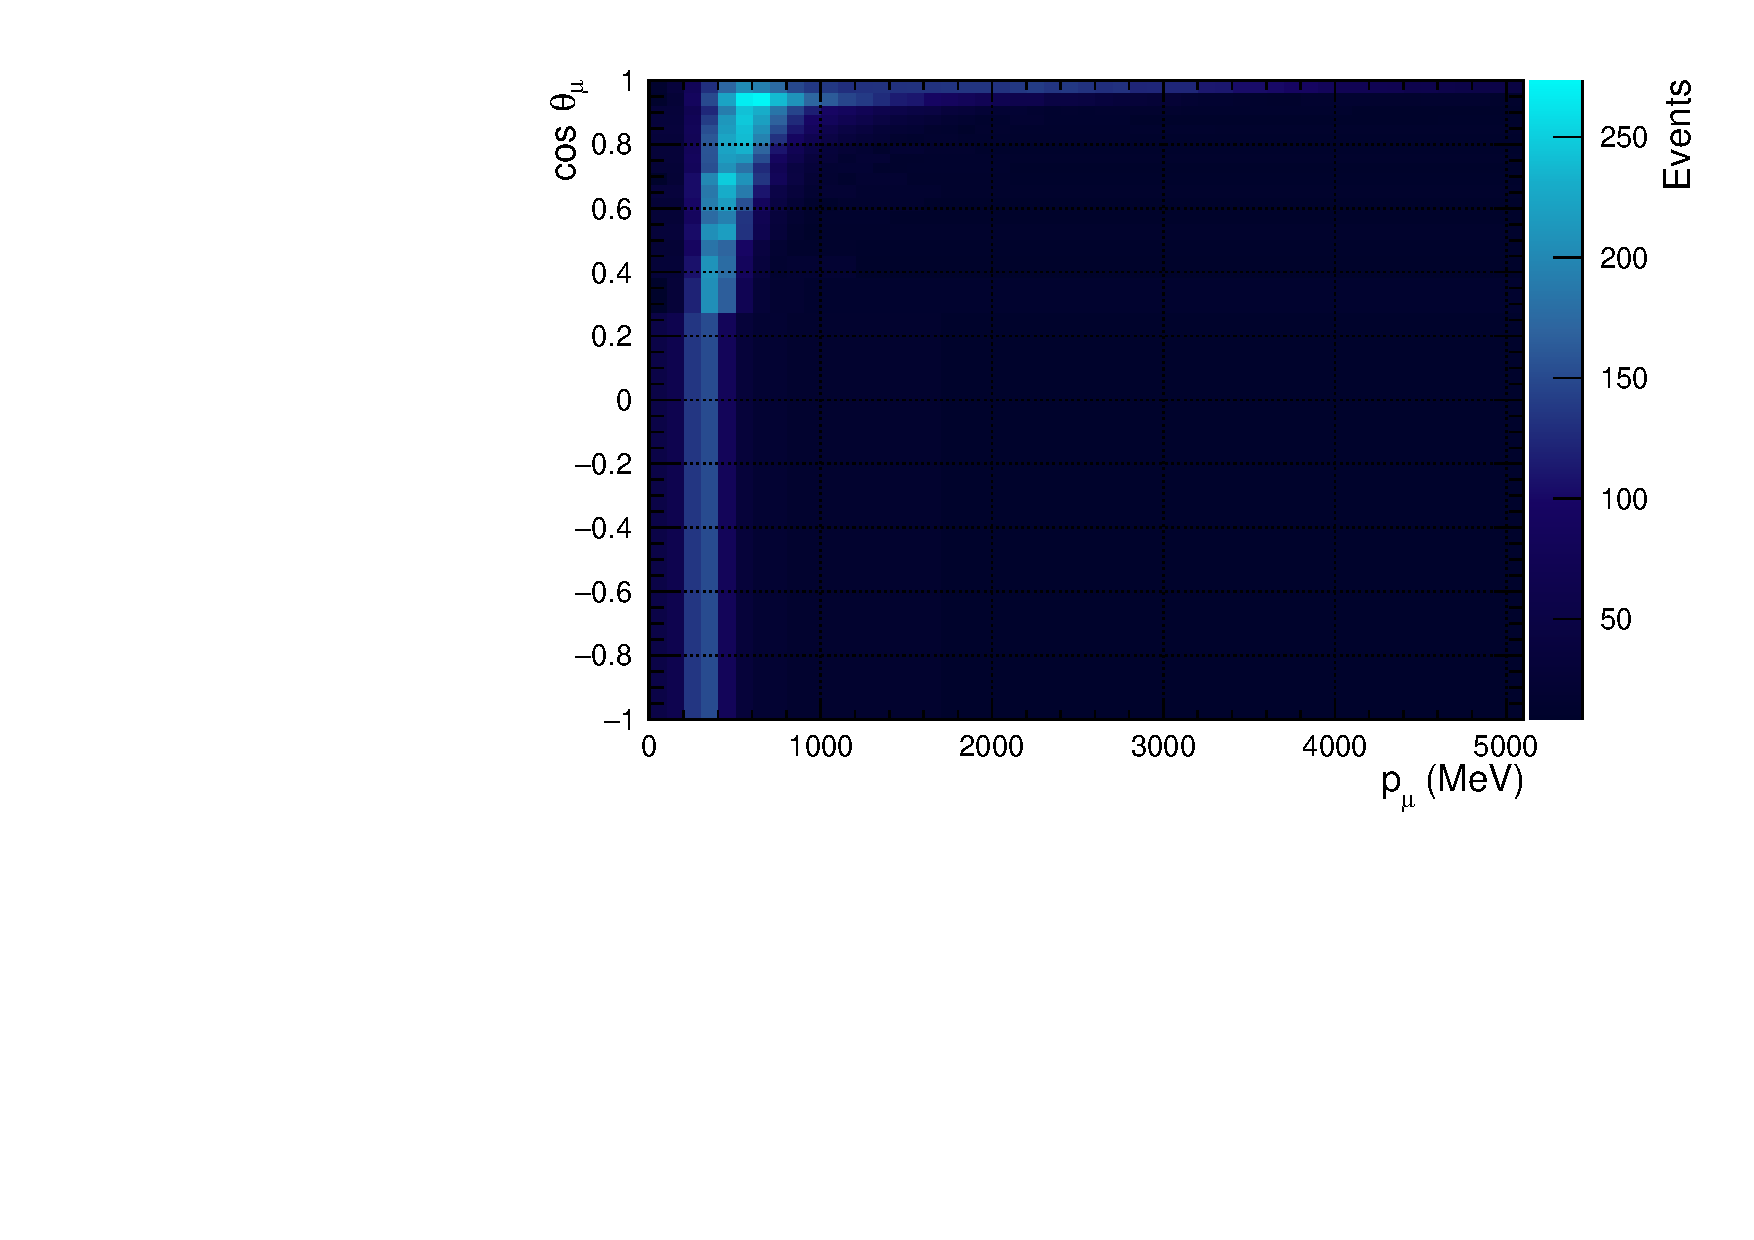
\includegraphics[width=0.95\linewidth]{figs/TH2PolyNom_MC_FGD1_numuCC_0pi}
  \caption{FGD1 FHC $\nu_{\mu}$ 0$\pi$}
  \label{fig:th2polynomFGD1_numuCC_0pi}
\end{subfigure}
\begin{subfigure}{.32\textwidth}
  \centering
  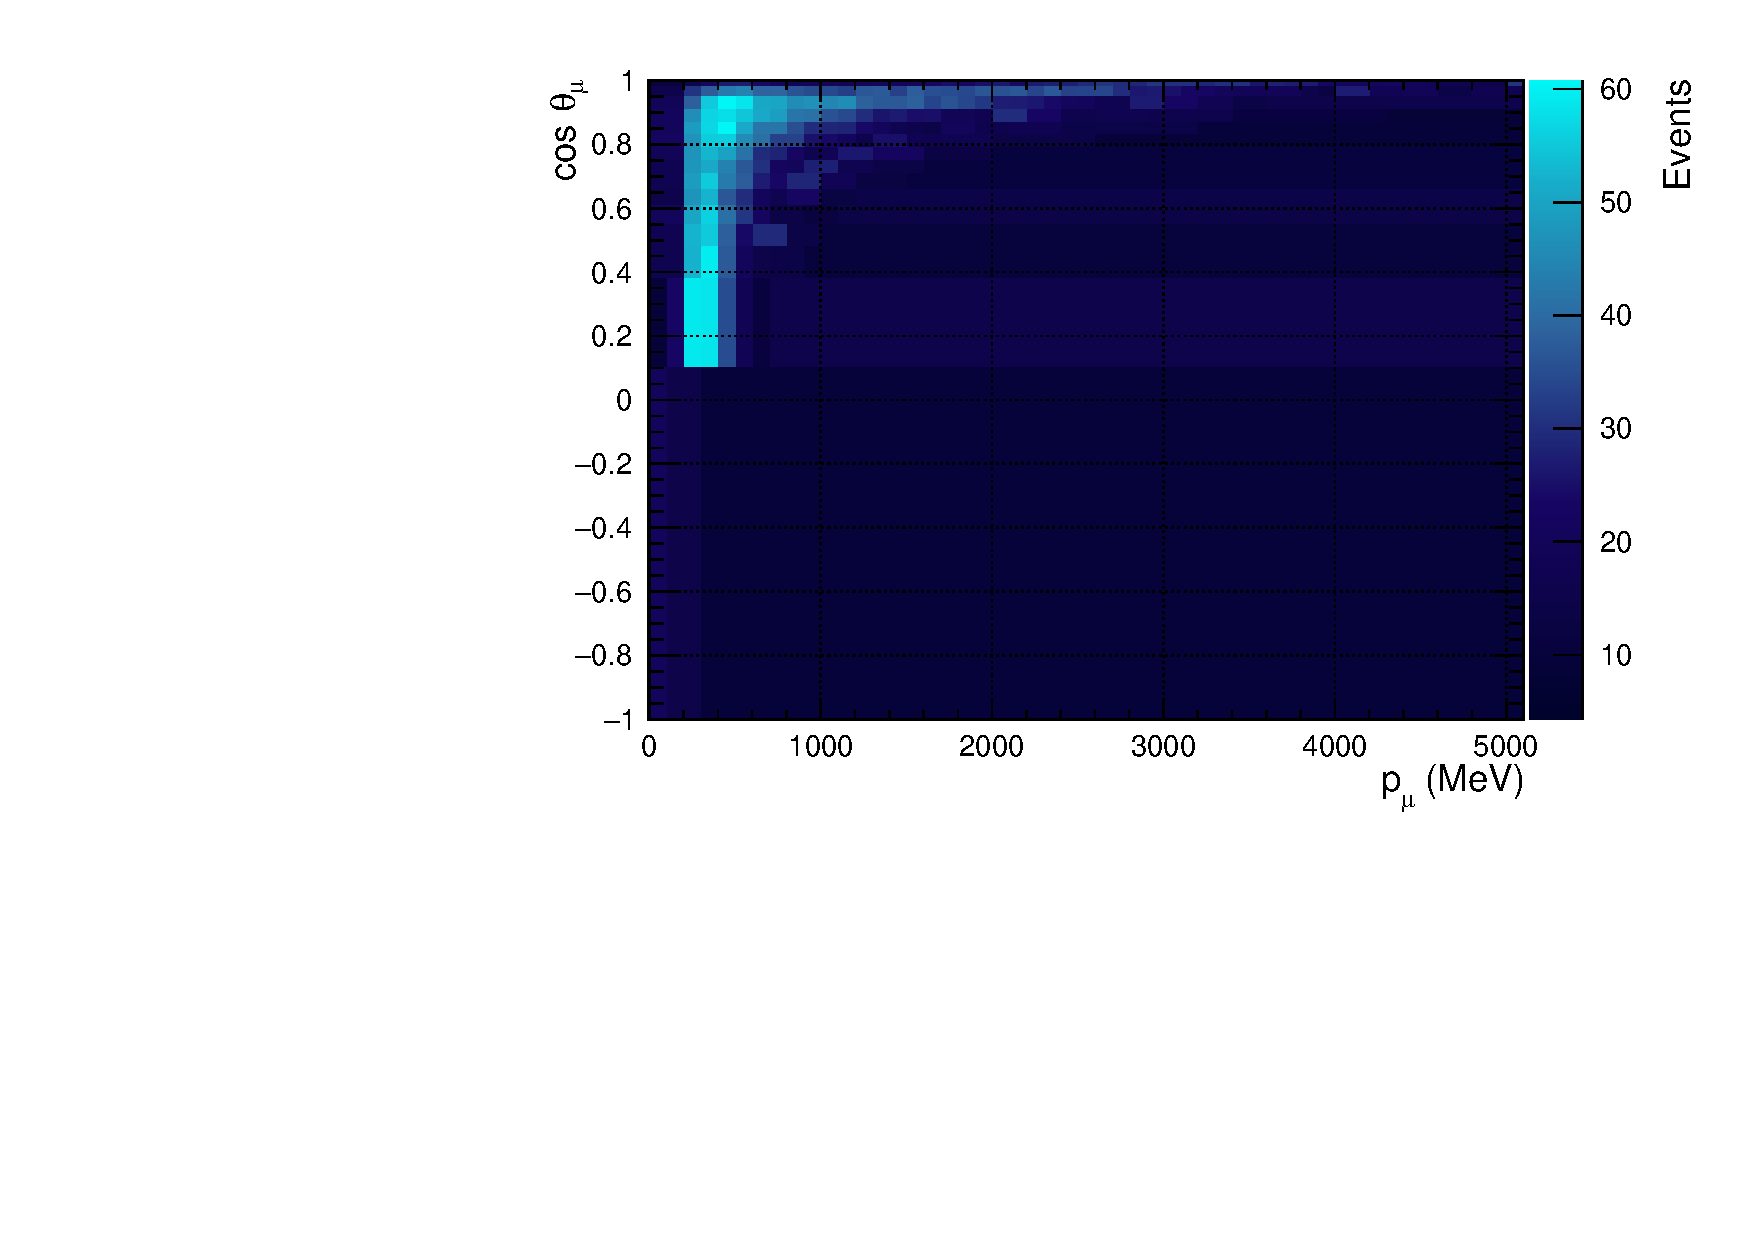
\includegraphics[width=0.95\linewidth]{figs/TH2PolyNom_MC_FGD1_numuCC_1pi}
  \caption{FGD1 FHC $\nu_{\mu}$ 1$\pi$}
  \label{fig:th2polynomFGD1_numuCC_1pi}
\end{subfigure}
\begin{subfigure}{.32\textwidth}
  \centering
  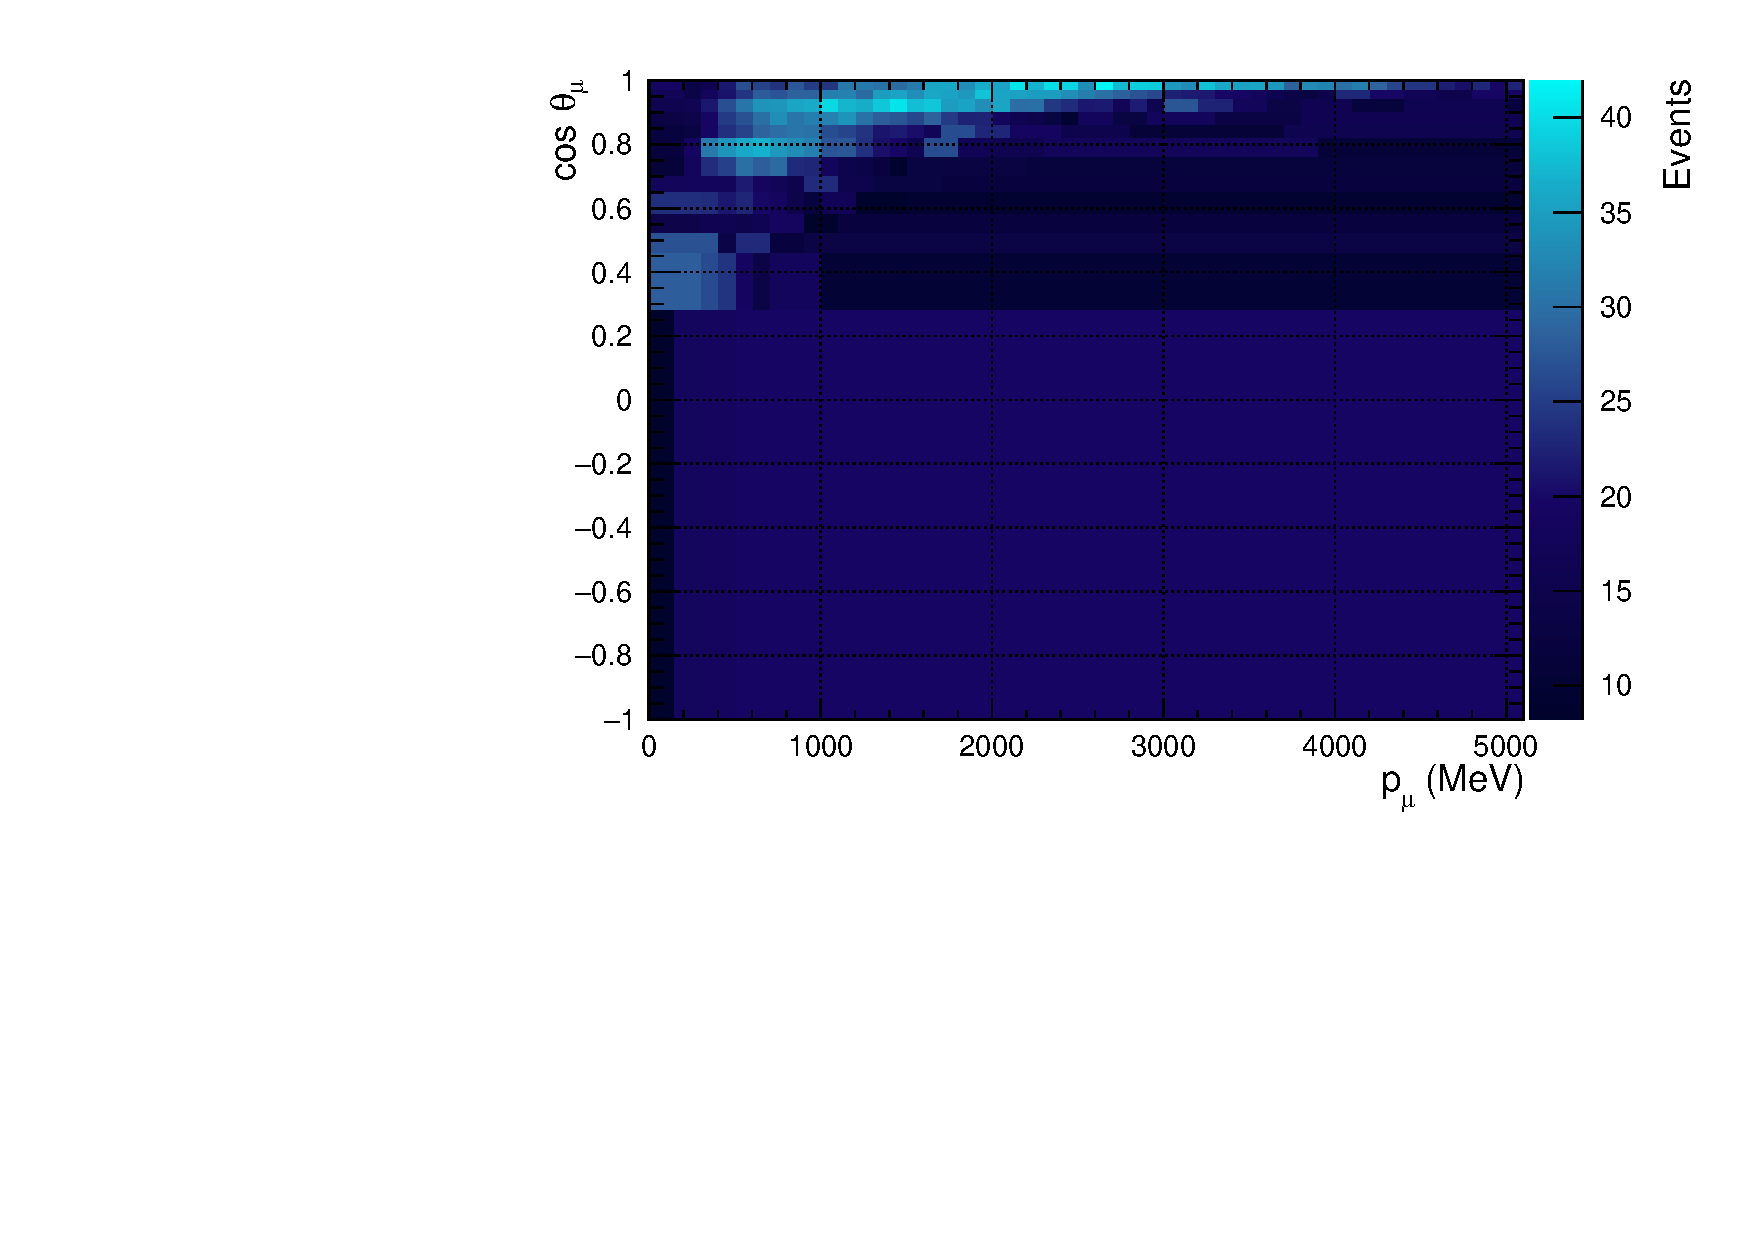
\includegraphics[width=0.95\linewidth]{figs/TH2PolyNom_MC_FGD1_numuCC_other}
  \caption{FGD1 FHC $\nu_{\mu}$ Other}
  \label{fig:th2polynomFGD1_numuCC_other}
\end{subfigure}
\centering
\begin{subfigure}{.32\textwidth}
  \centering
  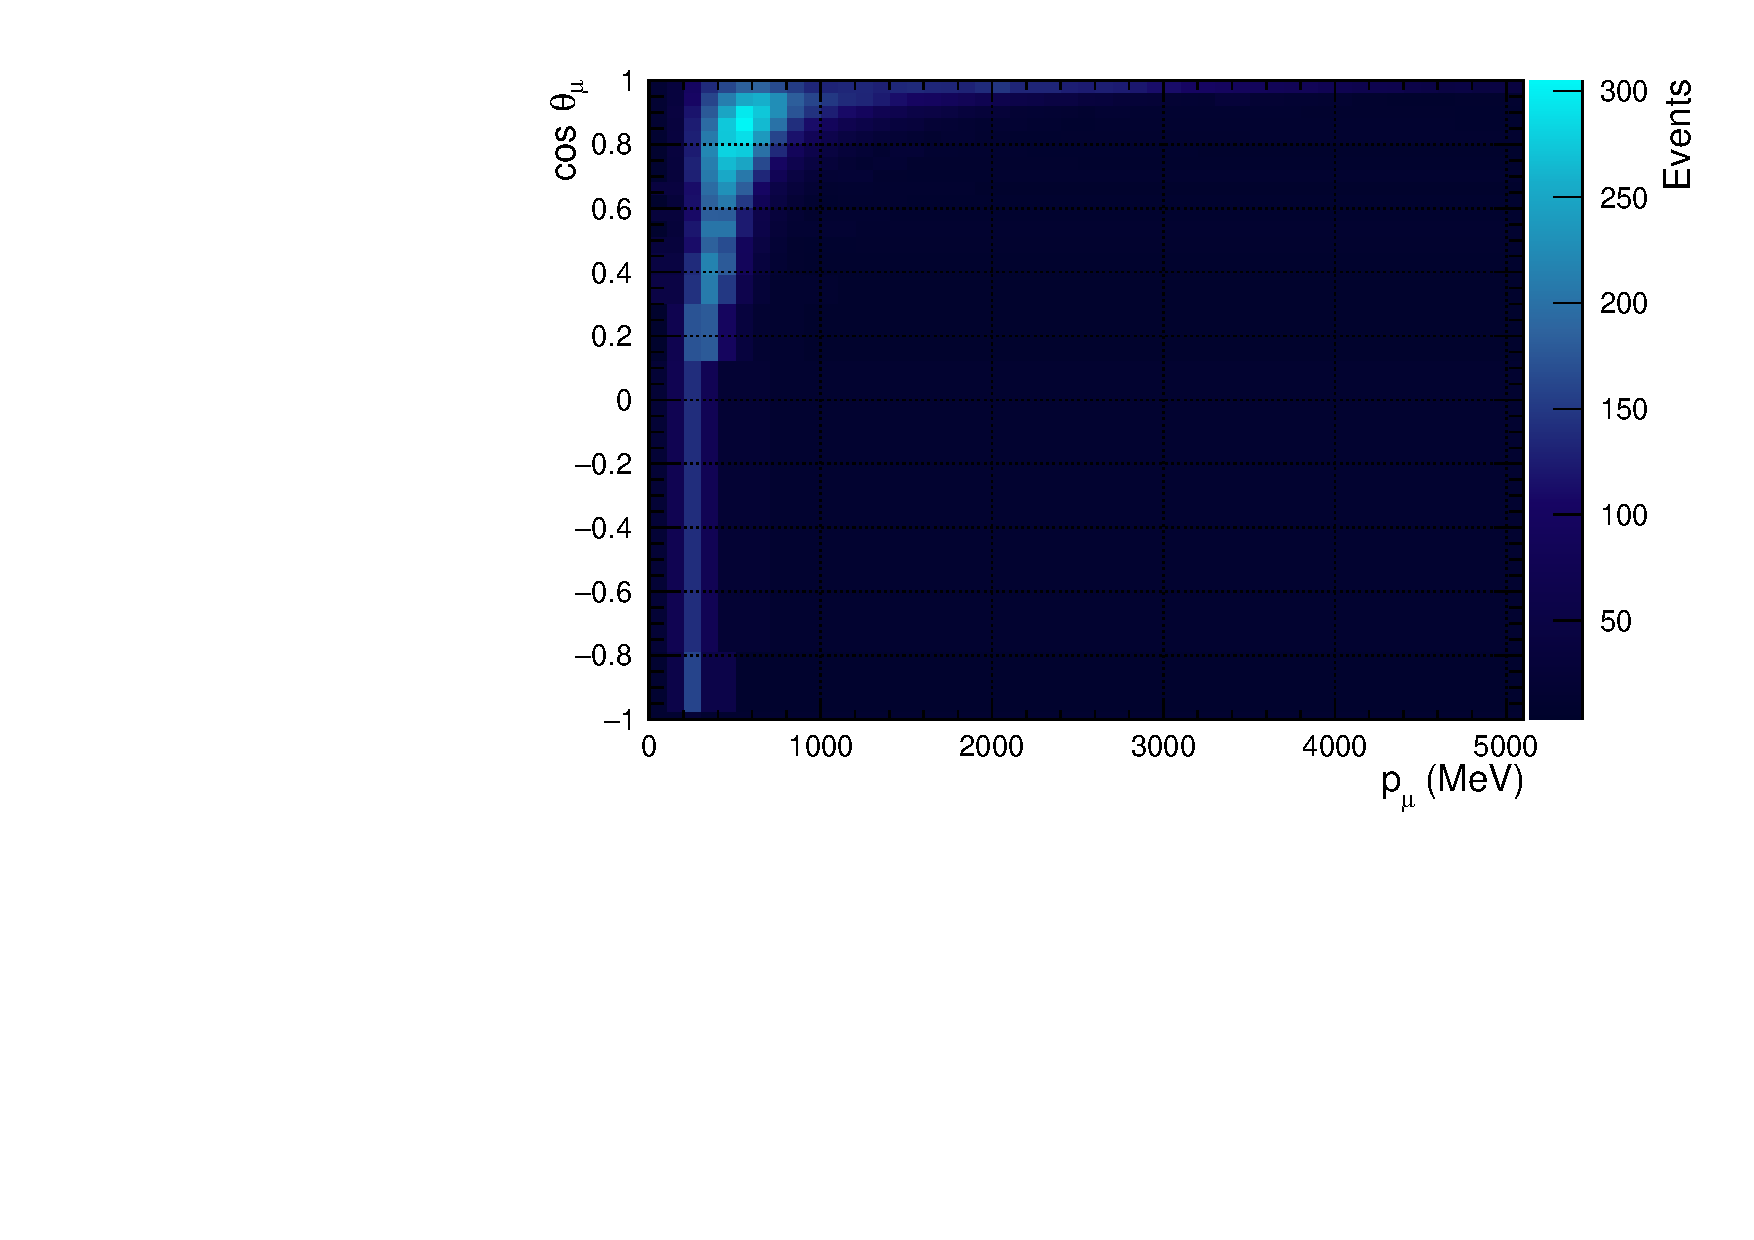
\includegraphics[width=0.95\linewidth]{figs/TH2PolyNom_MC_FGD2_numuCC_0pi}
  \caption{FGD2 FHC $\nu_{\mu}$ 0$\pi$}
  \label{fig:th2polynomFGD2_numuCC_0pi}
\end{subfigure}
\begin{subfigure}{.32\textwidth}
  \centering
  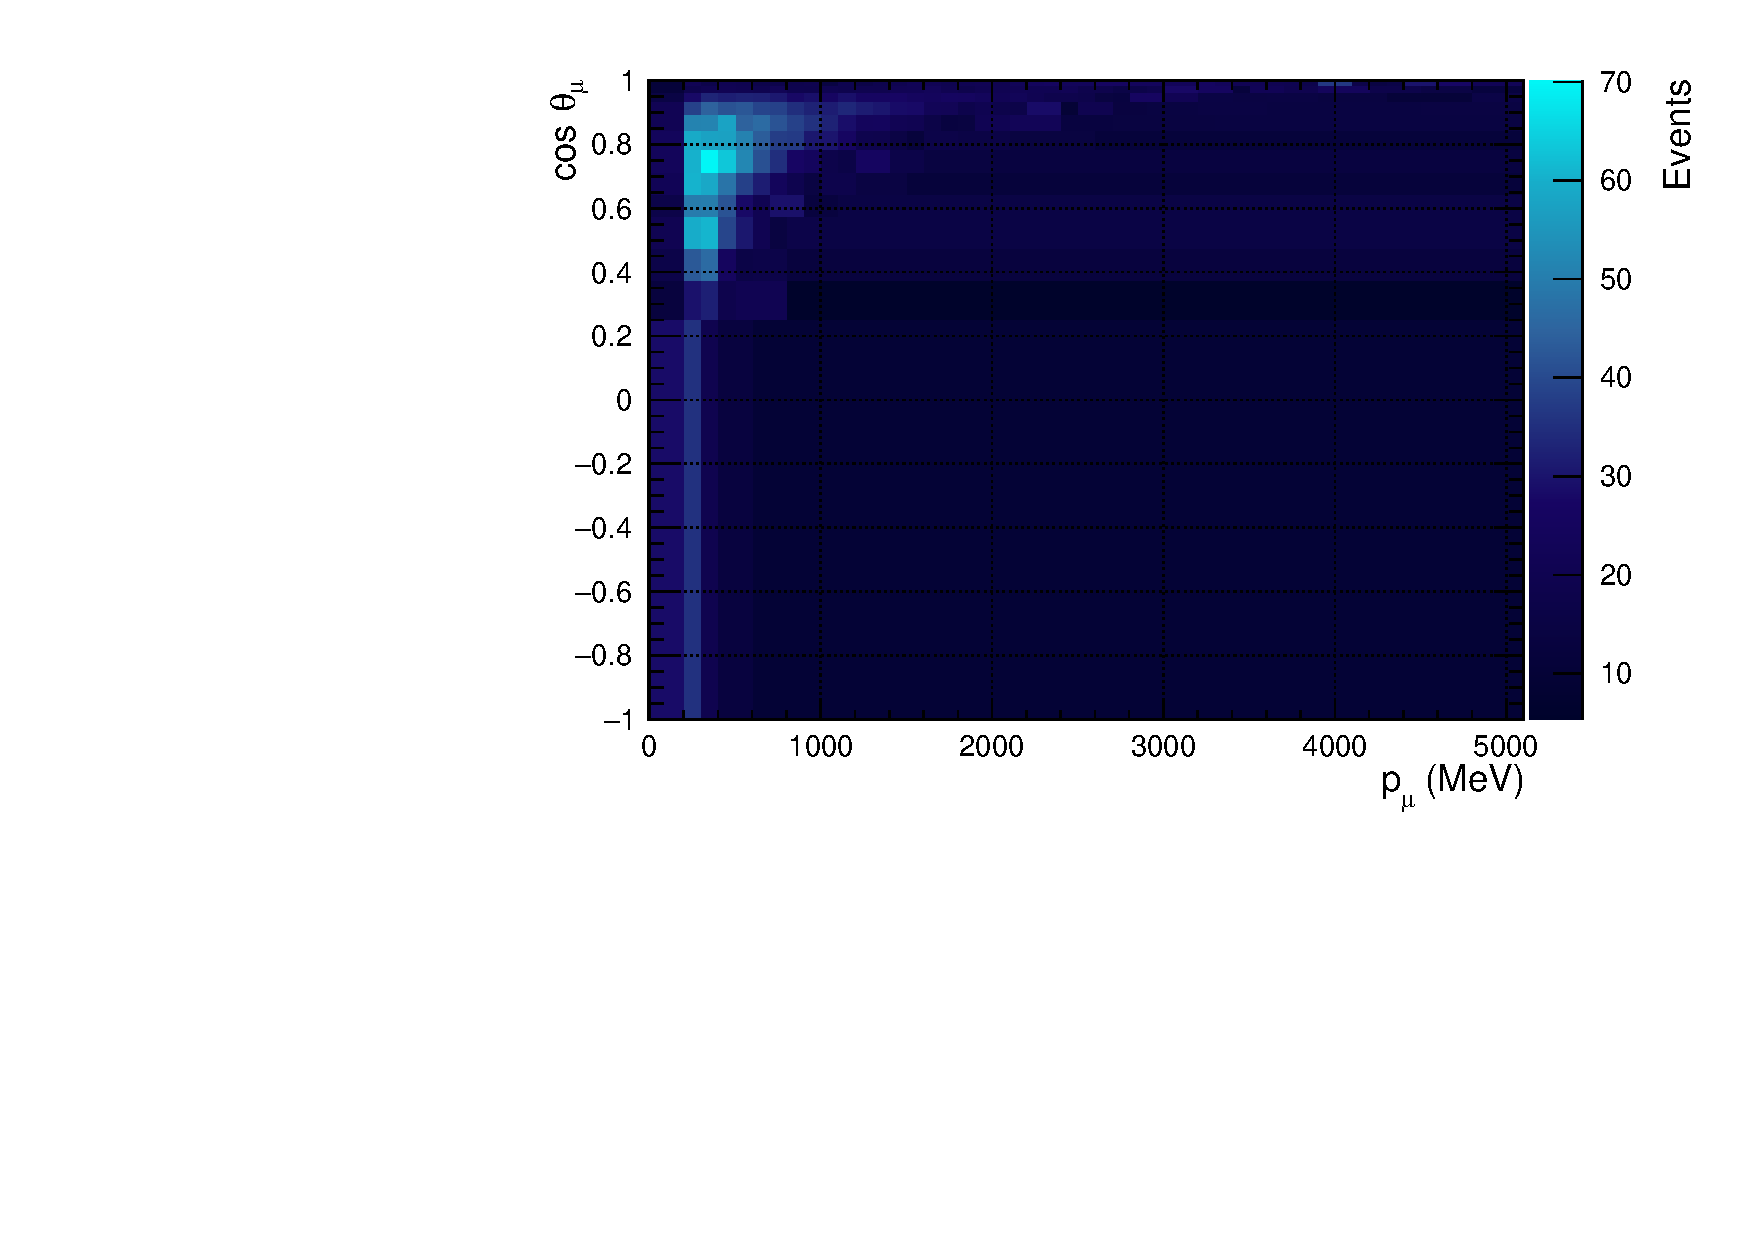
\includegraphics[width=0.95\linewidth]{figs/TH2PolyNom_MC_FGD2_numuCC_1pi}
  \caption{FGD2 FHC $\nu_{\mu}$ 1$\pi$}
  \label{fig:th2polynomFGD2_numuCC_1pi}
\end{subfigure}
\begin{subfigure}{.32\textwidth}
  \centering
  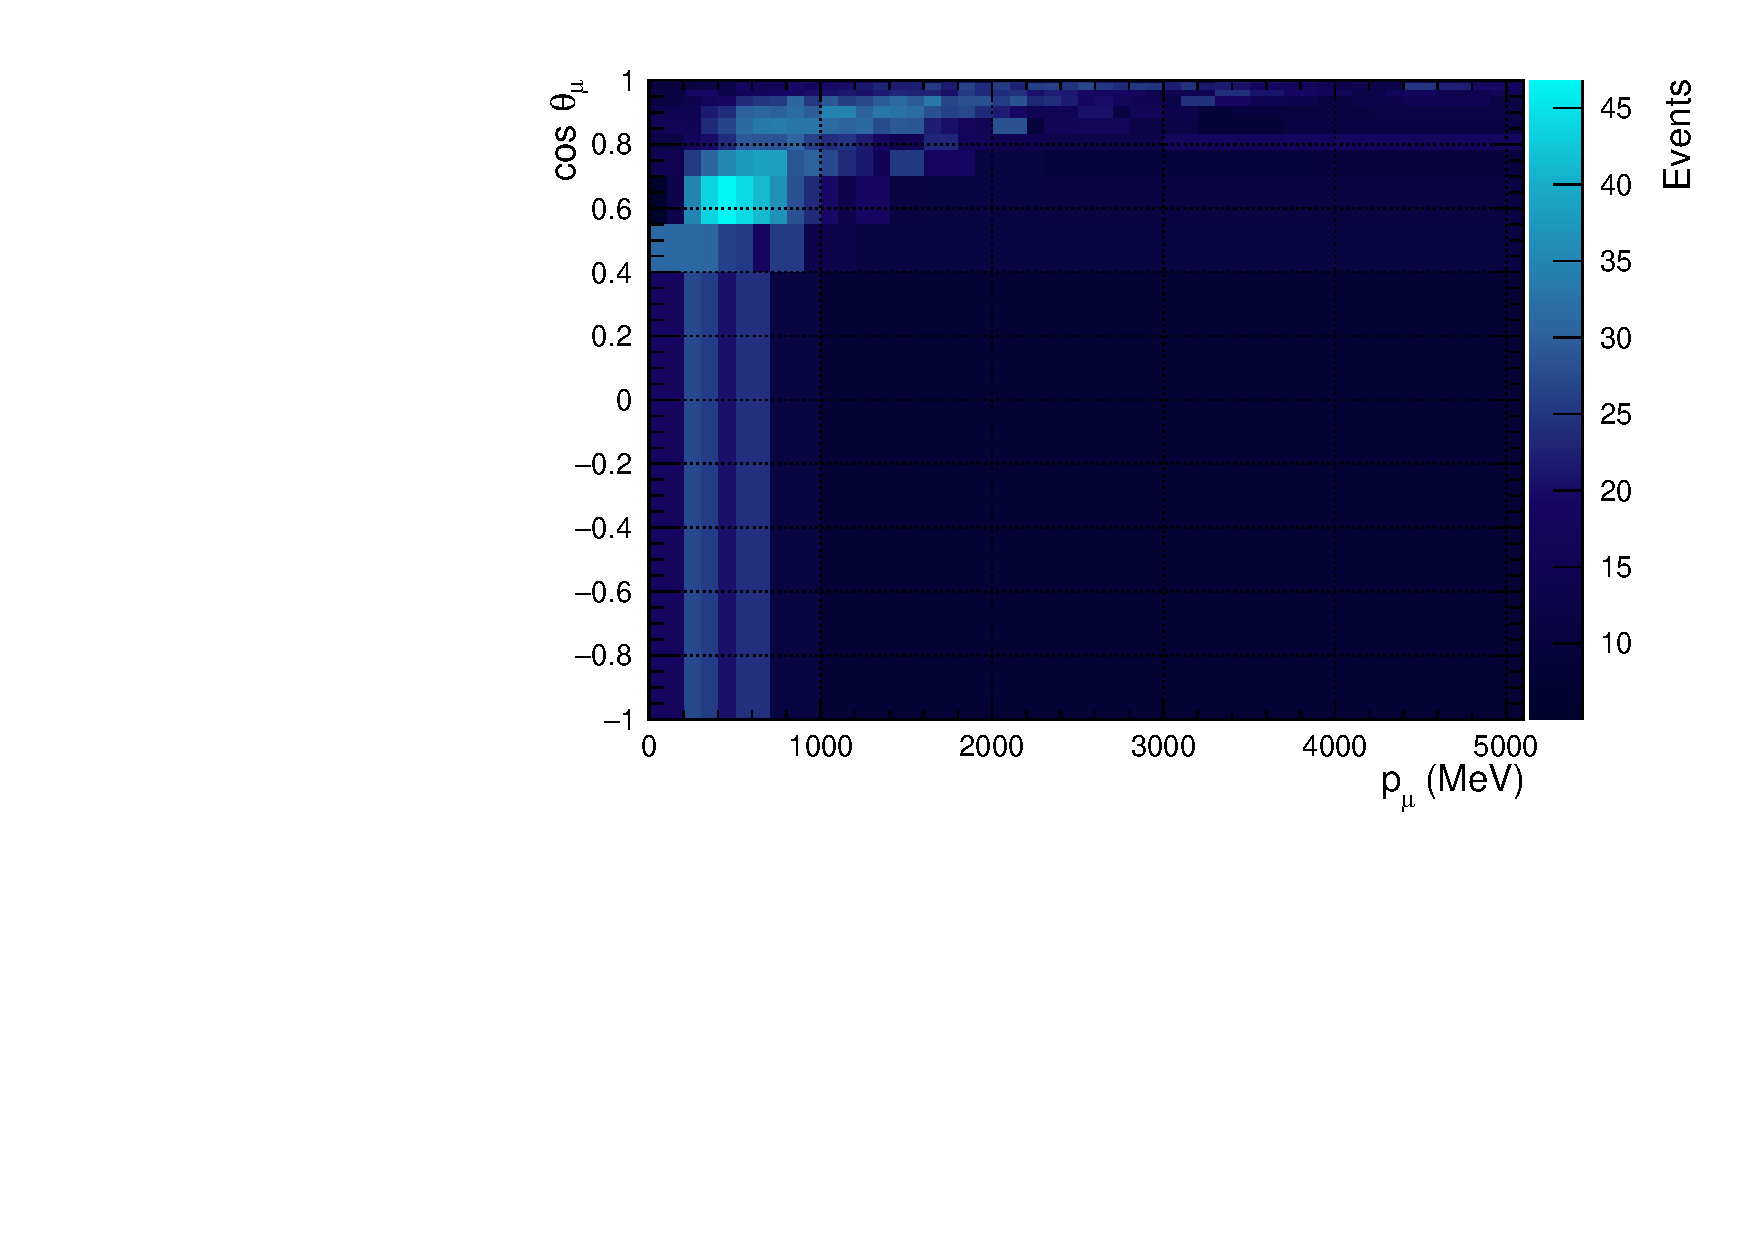
\includegraphics[width=0.95\linewidth]{figs/TH2PolyNom_MC_FGD2_numuCC_other}
  \caption{FGD2 FHC $\nu_{\mu}$ Other}
  \label{fig:th2polynomFGD2_numuCC_other}
\end{subfigure}
\centering
\begin{subfigure}{.32\textwidth}
  \centering
  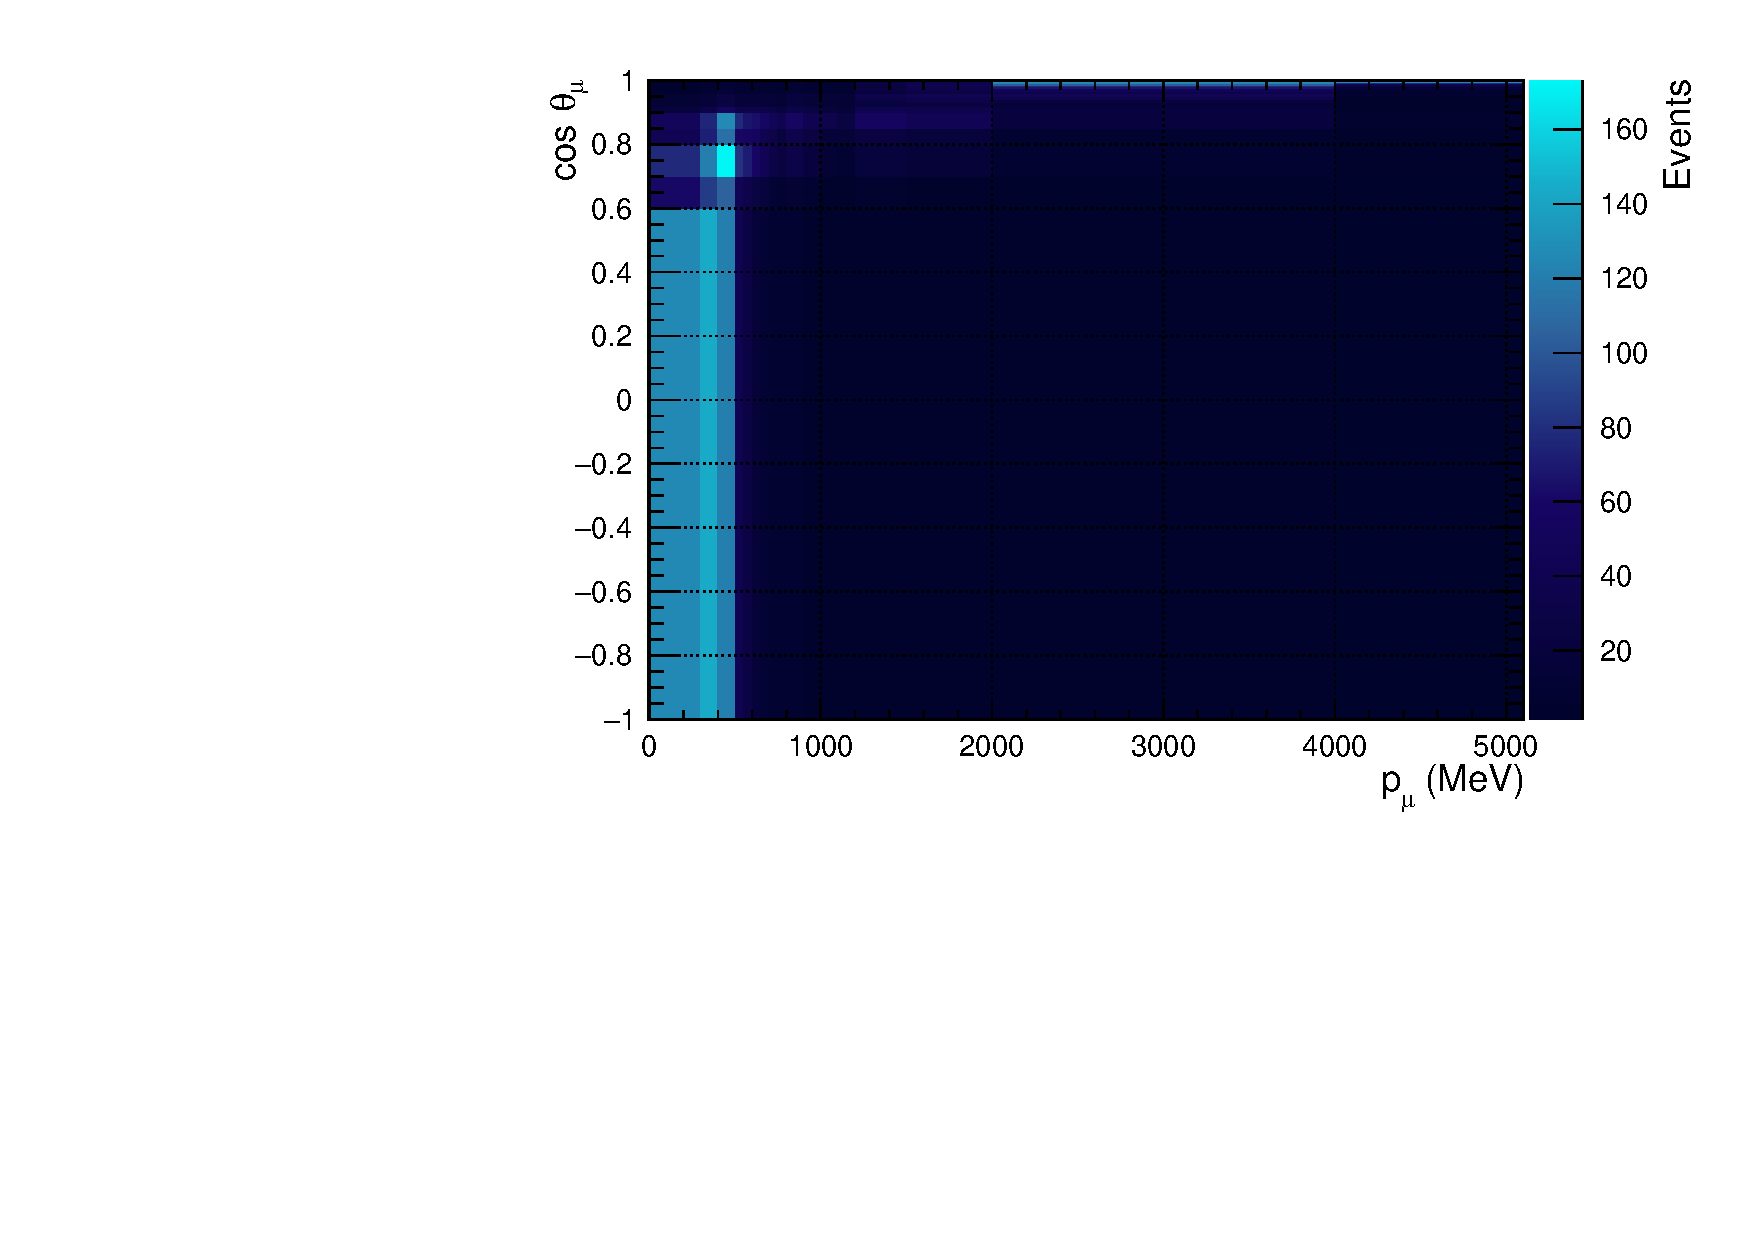
\includegraphics[width=0.95\linewidth]{figs/TH2PolyNom_MC_FGD1_anti-numuCC_0pi}
  \caption{FGD1 RHC $\bar{\nu_{\mu}}$ 0$\pi$}
  \label{fig:th2polynomFGD1_anti-numuCC_0pi}
\end{subfigure}
\begin{subfigure}{.32\textwidth}
  \centering
  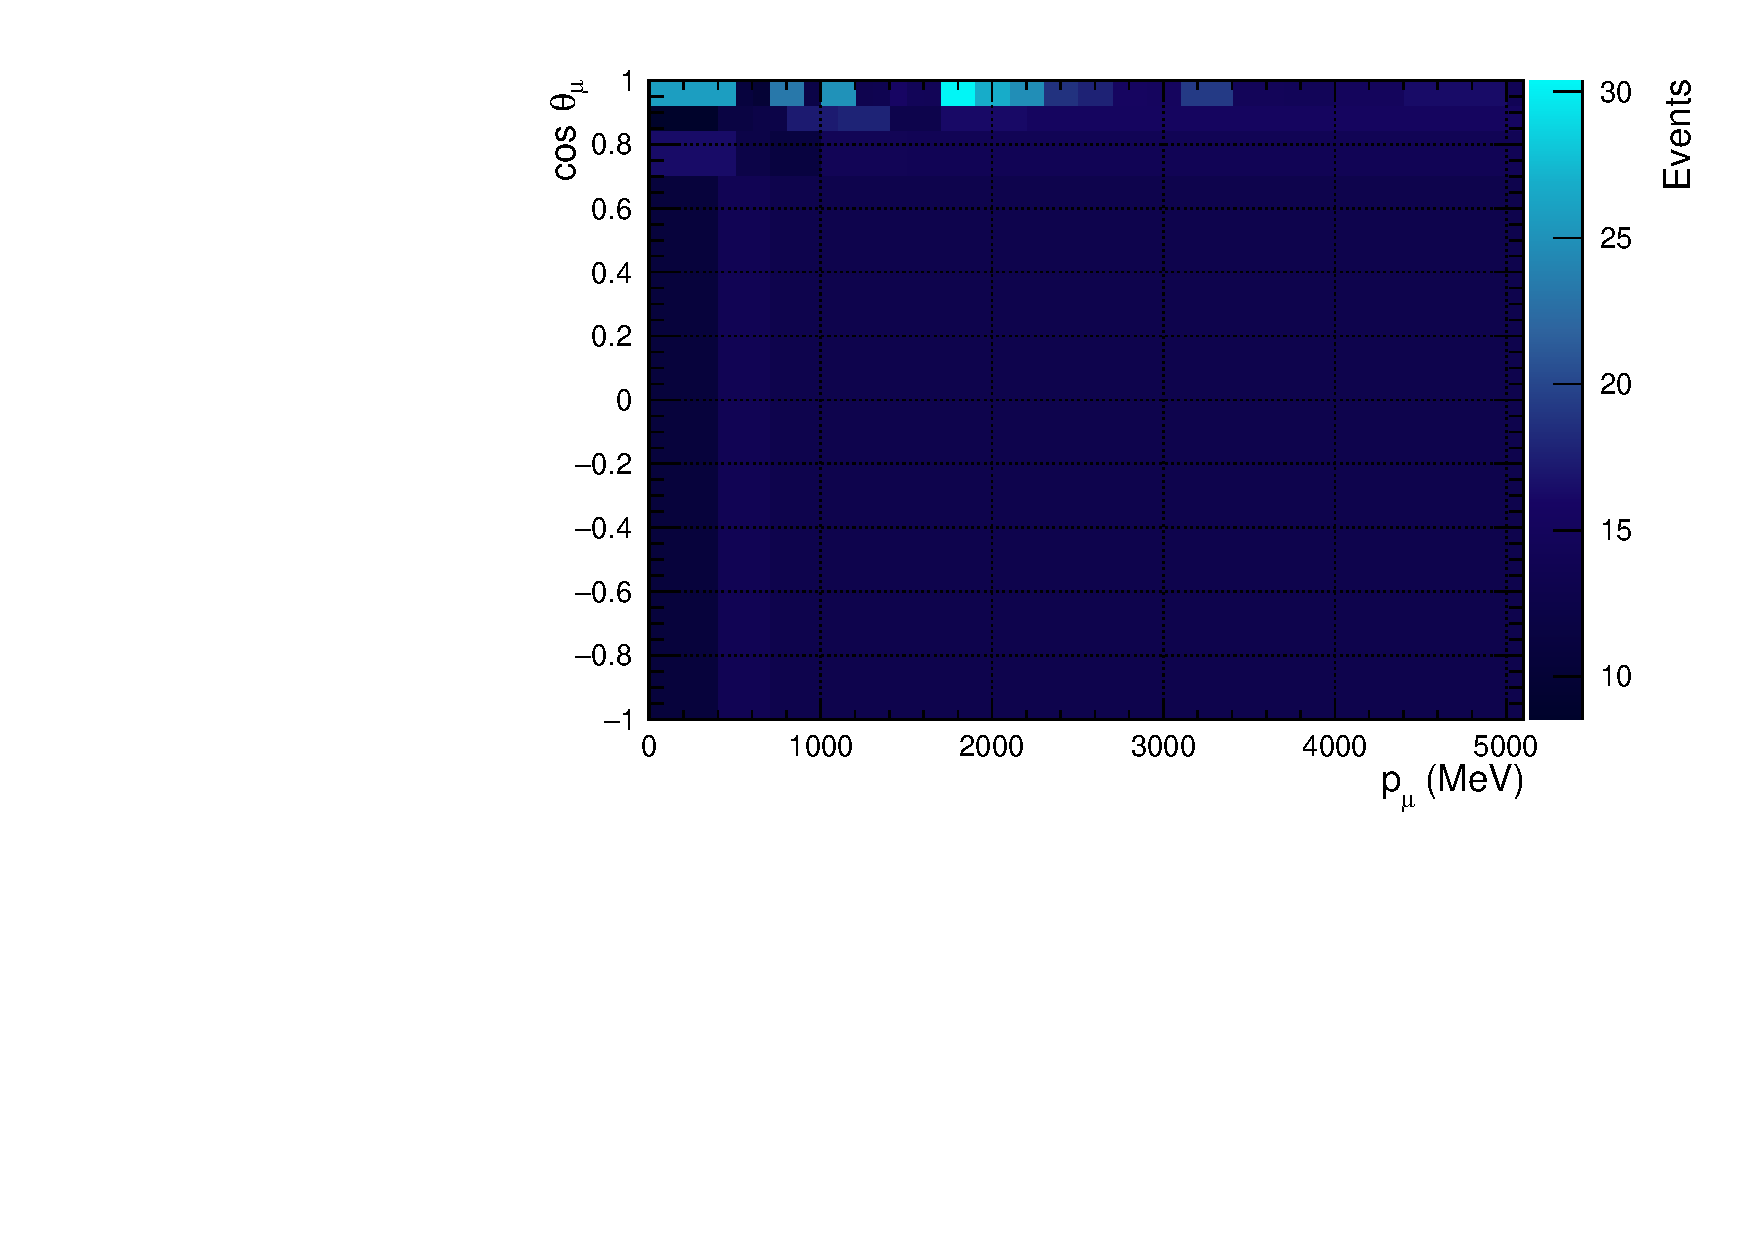
\includegraphics[width=0.95\linewidth]{figs/TH2PolyNom_MC_FGD1_anti-numuCC_1pi}
  \caption{FGD1 RHC $\bar{\nu_{\mu}}$ 1$\pi$}
  \label{fig:th2polyth2polynomFGD1_anti-numuCC_1pi}
\end{subfigure}
\begin{subfigure}{.32\textwidth}
  \centering
  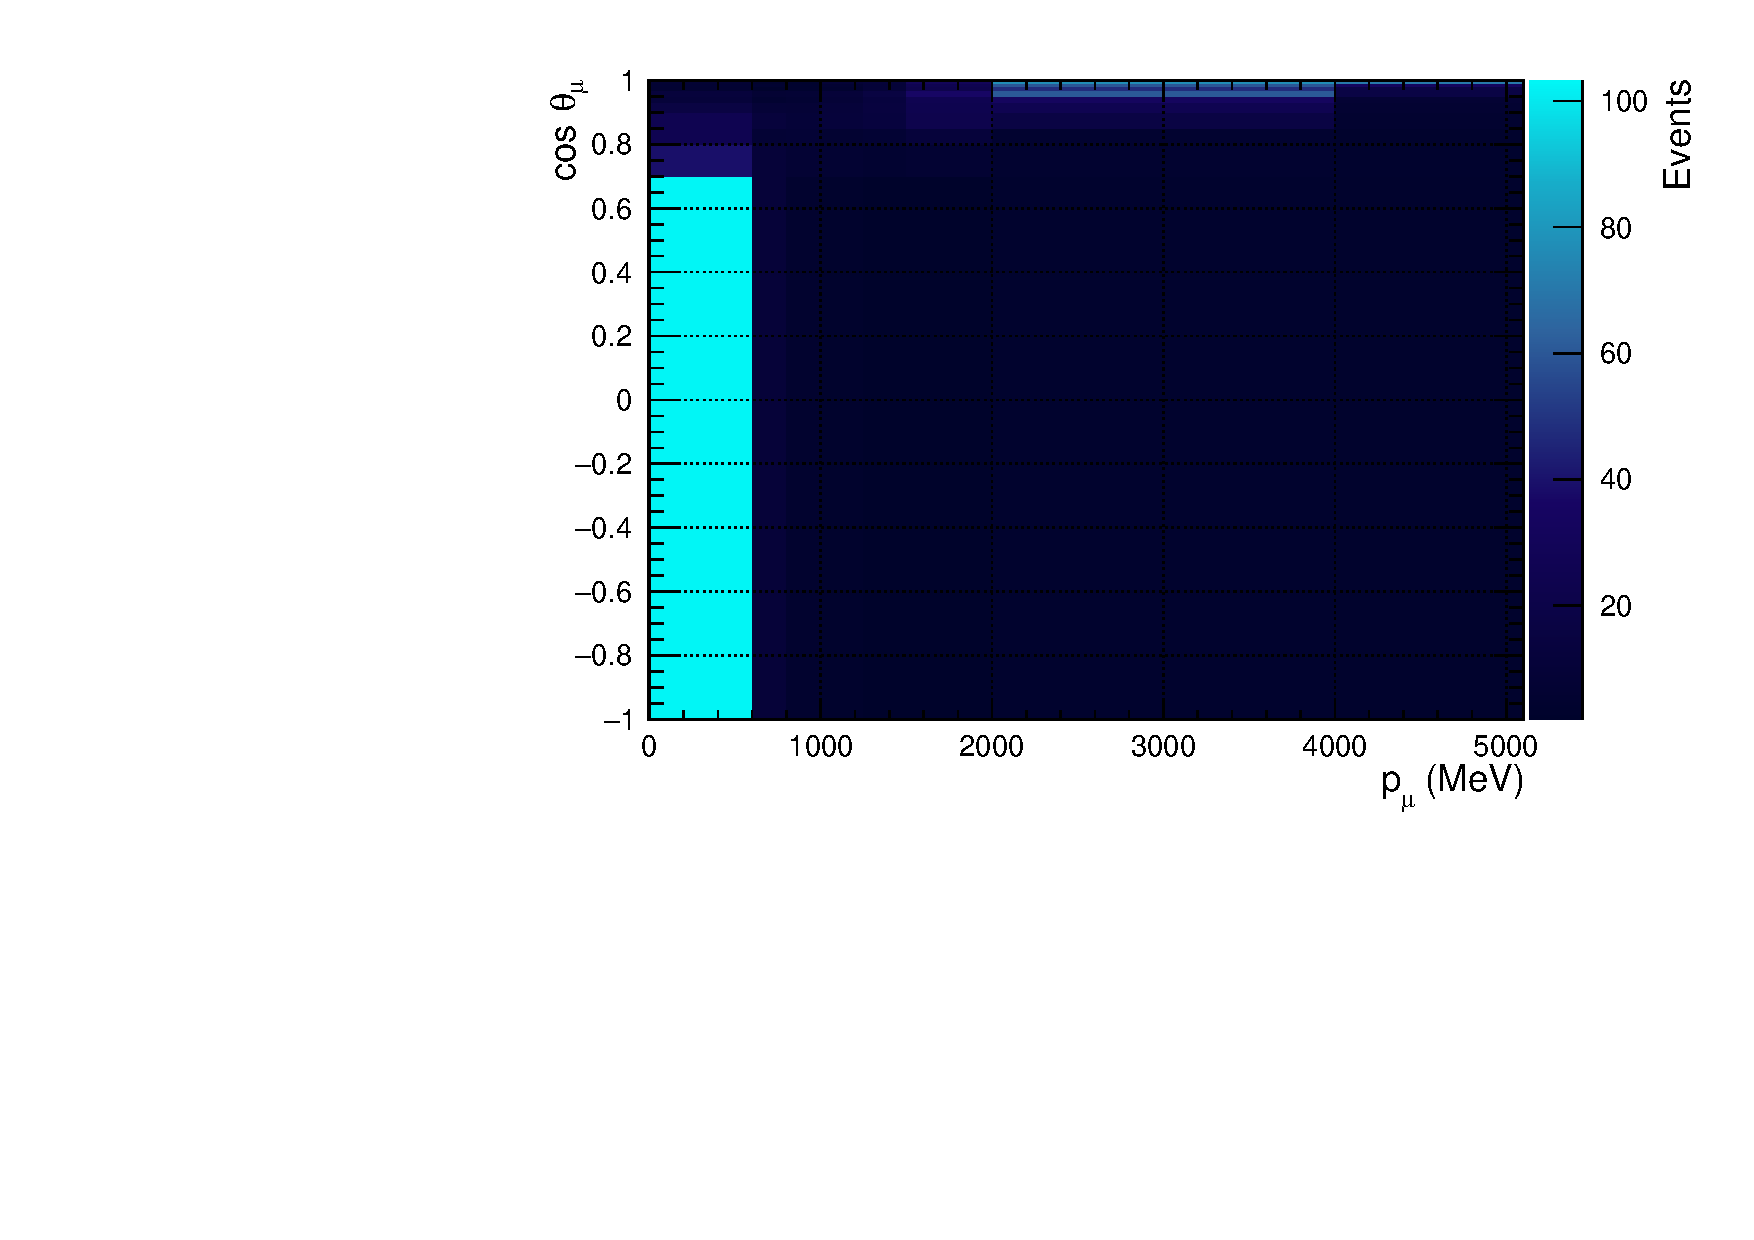
\includegraphics[width=0.95\linewidth]{figs/TH2PolyNom_MC_FGD1_anti-numuCC_other}
  \caption{FGD1 RHC $\bar{\nu_{\mu}}$ Other}
  \label{fig:th2polynomFGD1_anti-numuCC_other}
\end{subfigure}
\centering
\begin{subfigure}{.32\textwidth}
  \centering
  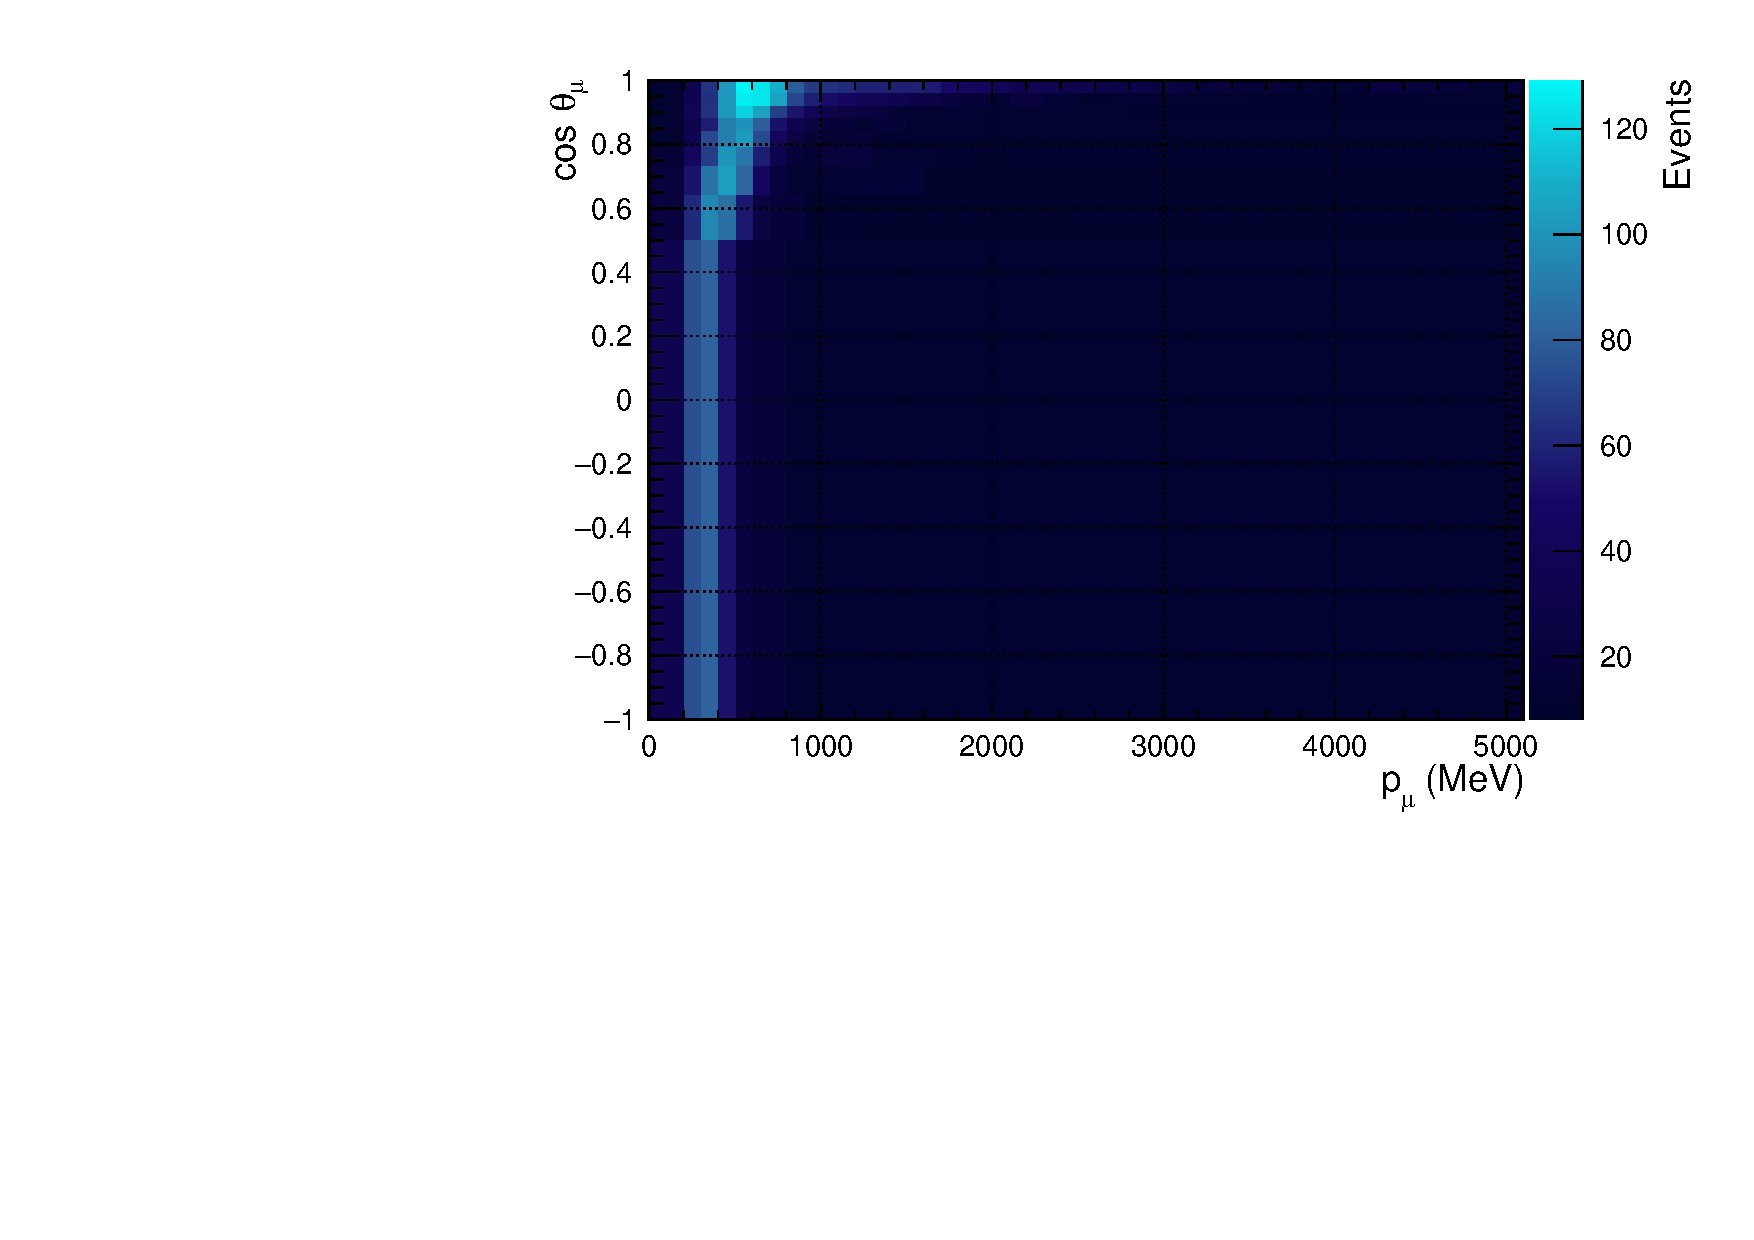
\includegraphics[width=0.95\linewidth]{figs/TH2PolyNom_MC_FGD2_anti-numuCC_0pi}
  \caption{FGD2 RHC $\bar{\nu_{\mu}}$ 0$\pi$}
  \label{fig:th2polynomFGD2_anti-numuCC_0pi}
\end{subfigure}
\begin{subfigure}{.32\textwidth}
  \centering
  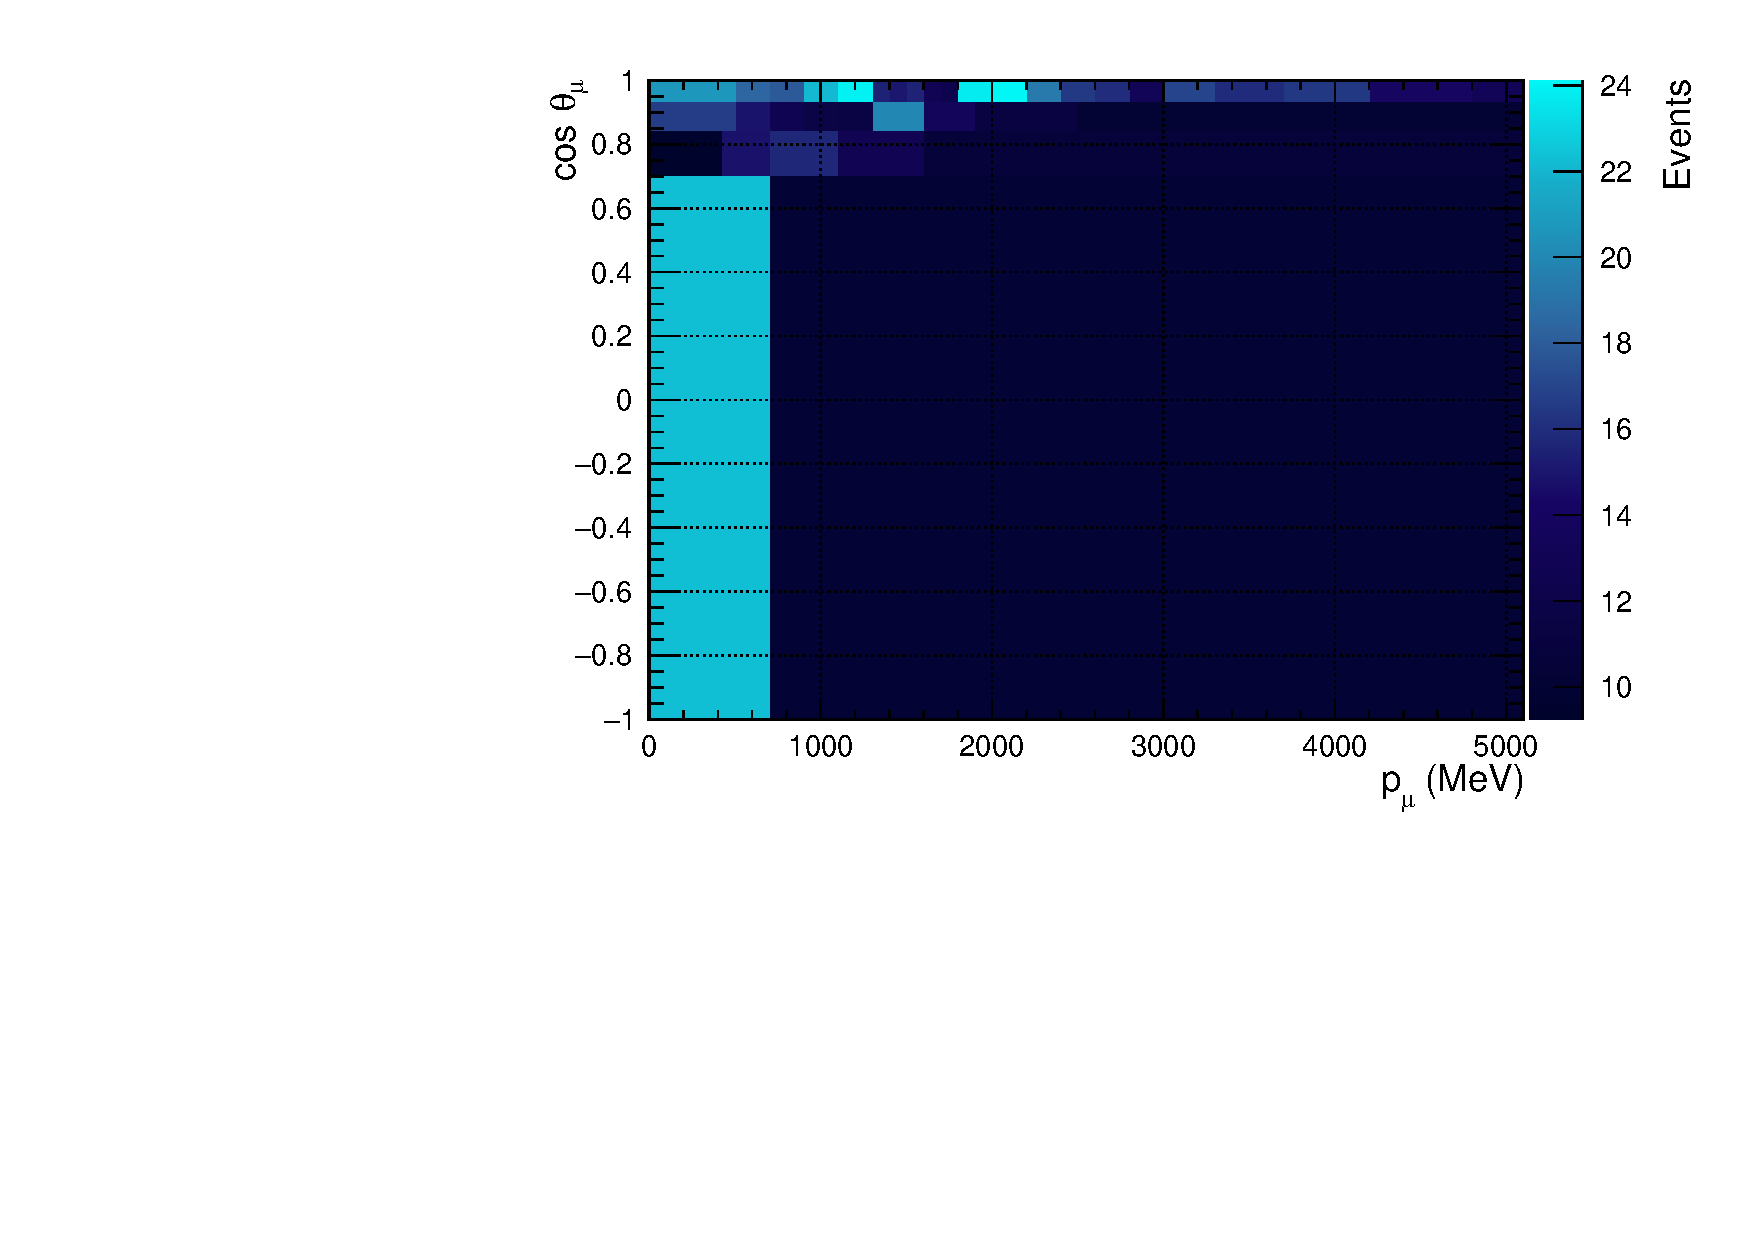
\includegraphics[width=0.95\linewidth]{figs/TH2PolyNom_MC_FGD2_anti-numuCC_1pi}
  \caption{FGD2 RHC $\bar{\nu_{\mu}}$ 1$\pi$}
  \label{fig:th2polyth2polynomFGD2_anti-numuCC_1pi}
\end{subfigure}
\begin{subfigure}{.32\textwidth}
  \centering
  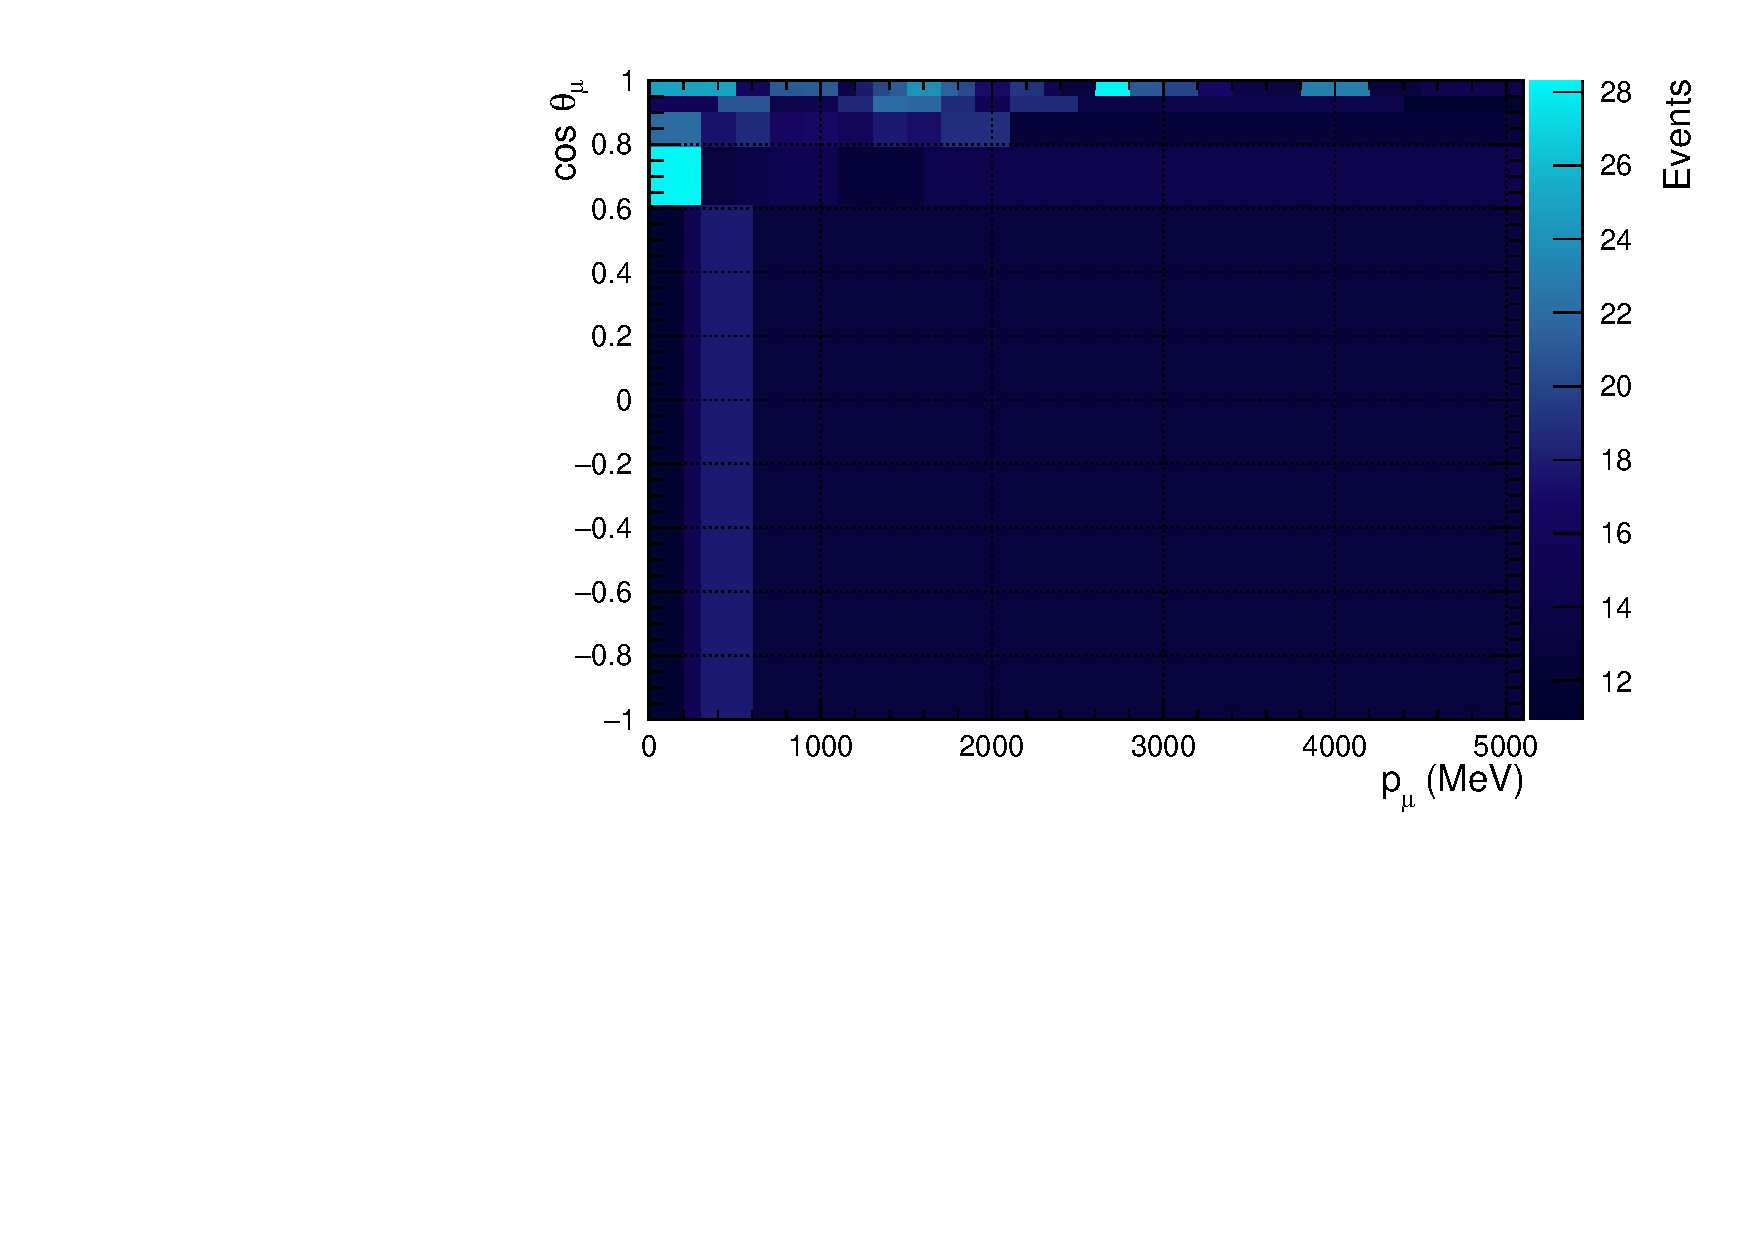
\includegraphics[width=0.95\linewidth]{figs/TH2PolyNom_MC_FGD2_anti-numuCC_other}
  \caption{FGD2 RHC $\bar{\nu_{\mu}}$ Other}
  \label{fig:th2polynomFGD2_anti-numuCC_other}
\end{subfigure}
\begin{subfigure}{.32\textwidth}
  \centering
  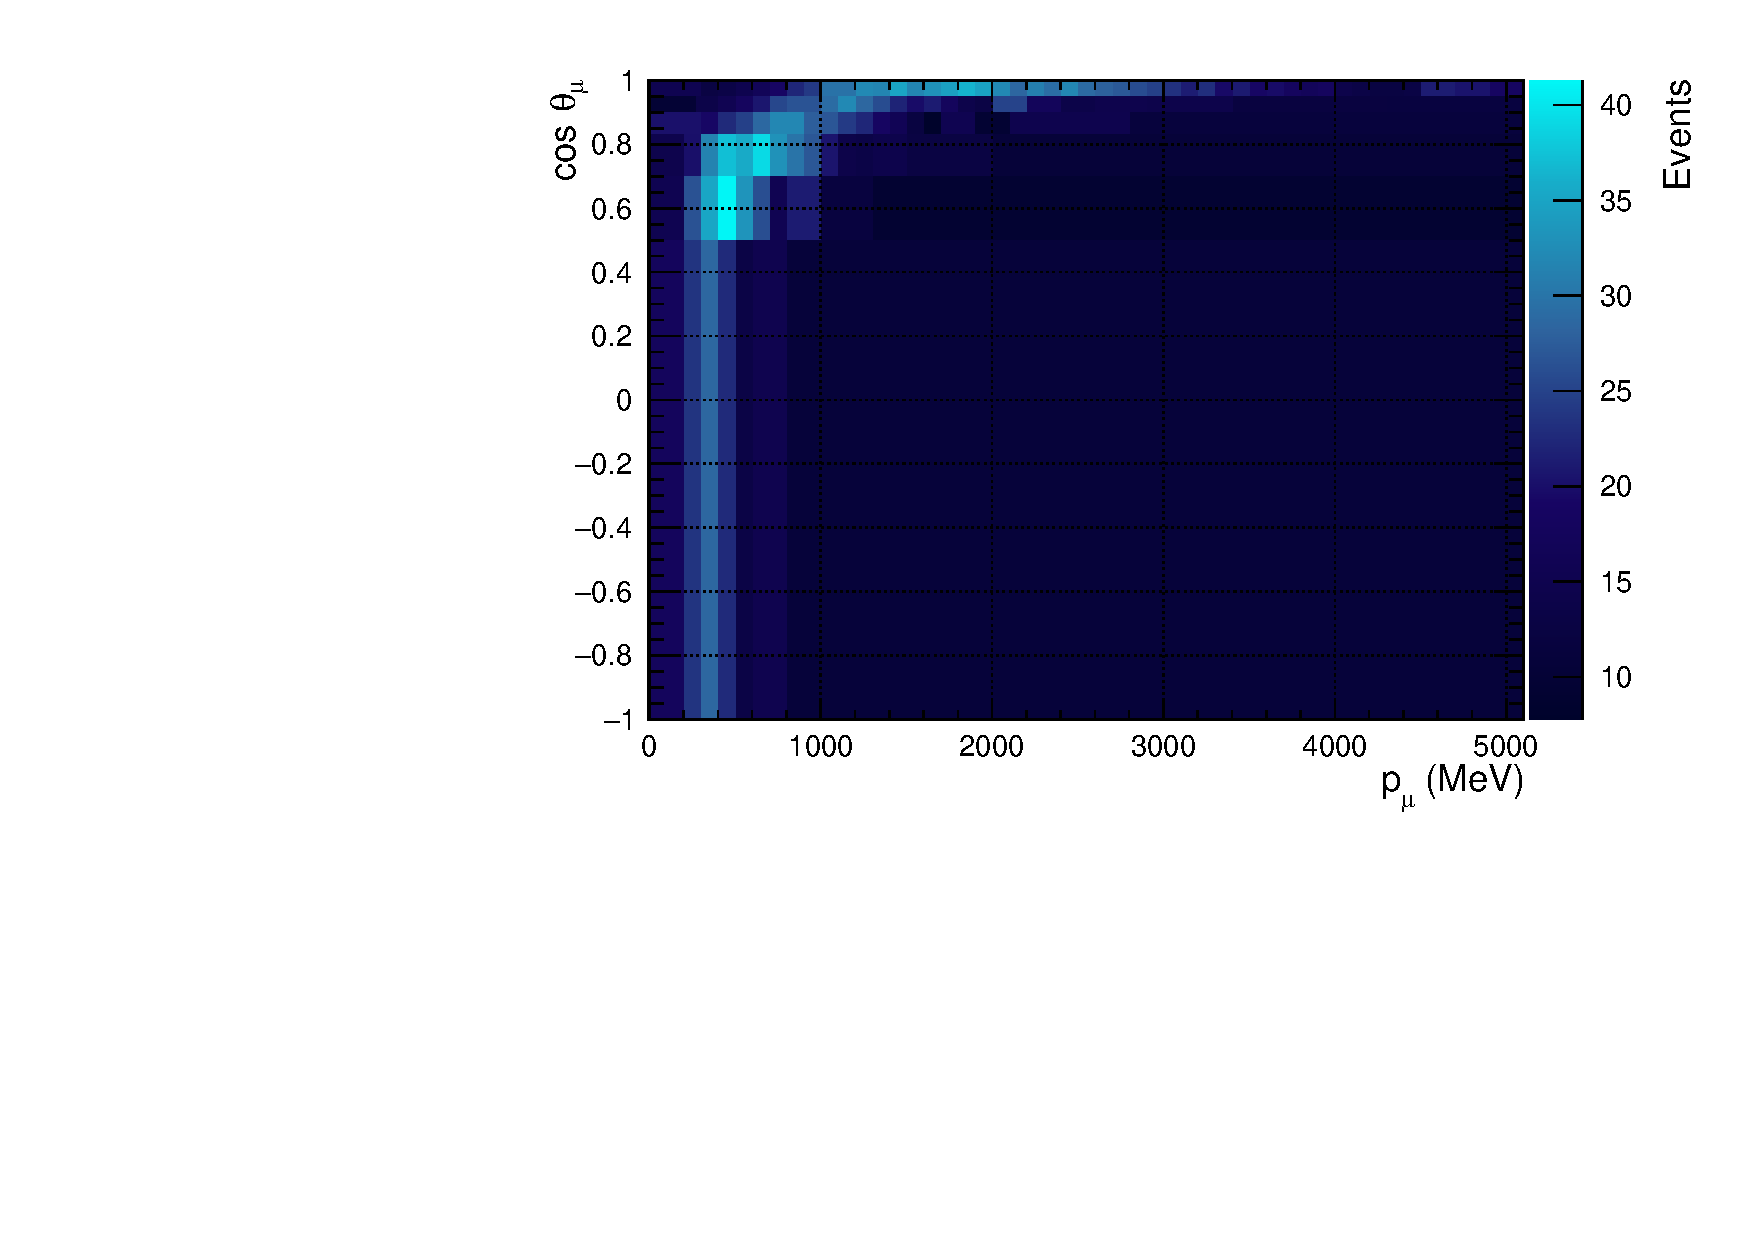
\includegraphics[width=0.95\linewidth]{figs/TH2PolyNom_MC_FGD1_NuMuBkg_CC0pi_in_AntiNu_Mode}
  \caption{FGD1 RHC $\nu_{\mu}$ 0$\pi$}
  \label{fig:th2polynomFGD1_NuMuBkg_CC0pi_in_AntiNu_Mode}
\end{subfigure}
\begin{subfigure}{.32\textwidth}
  \centering
  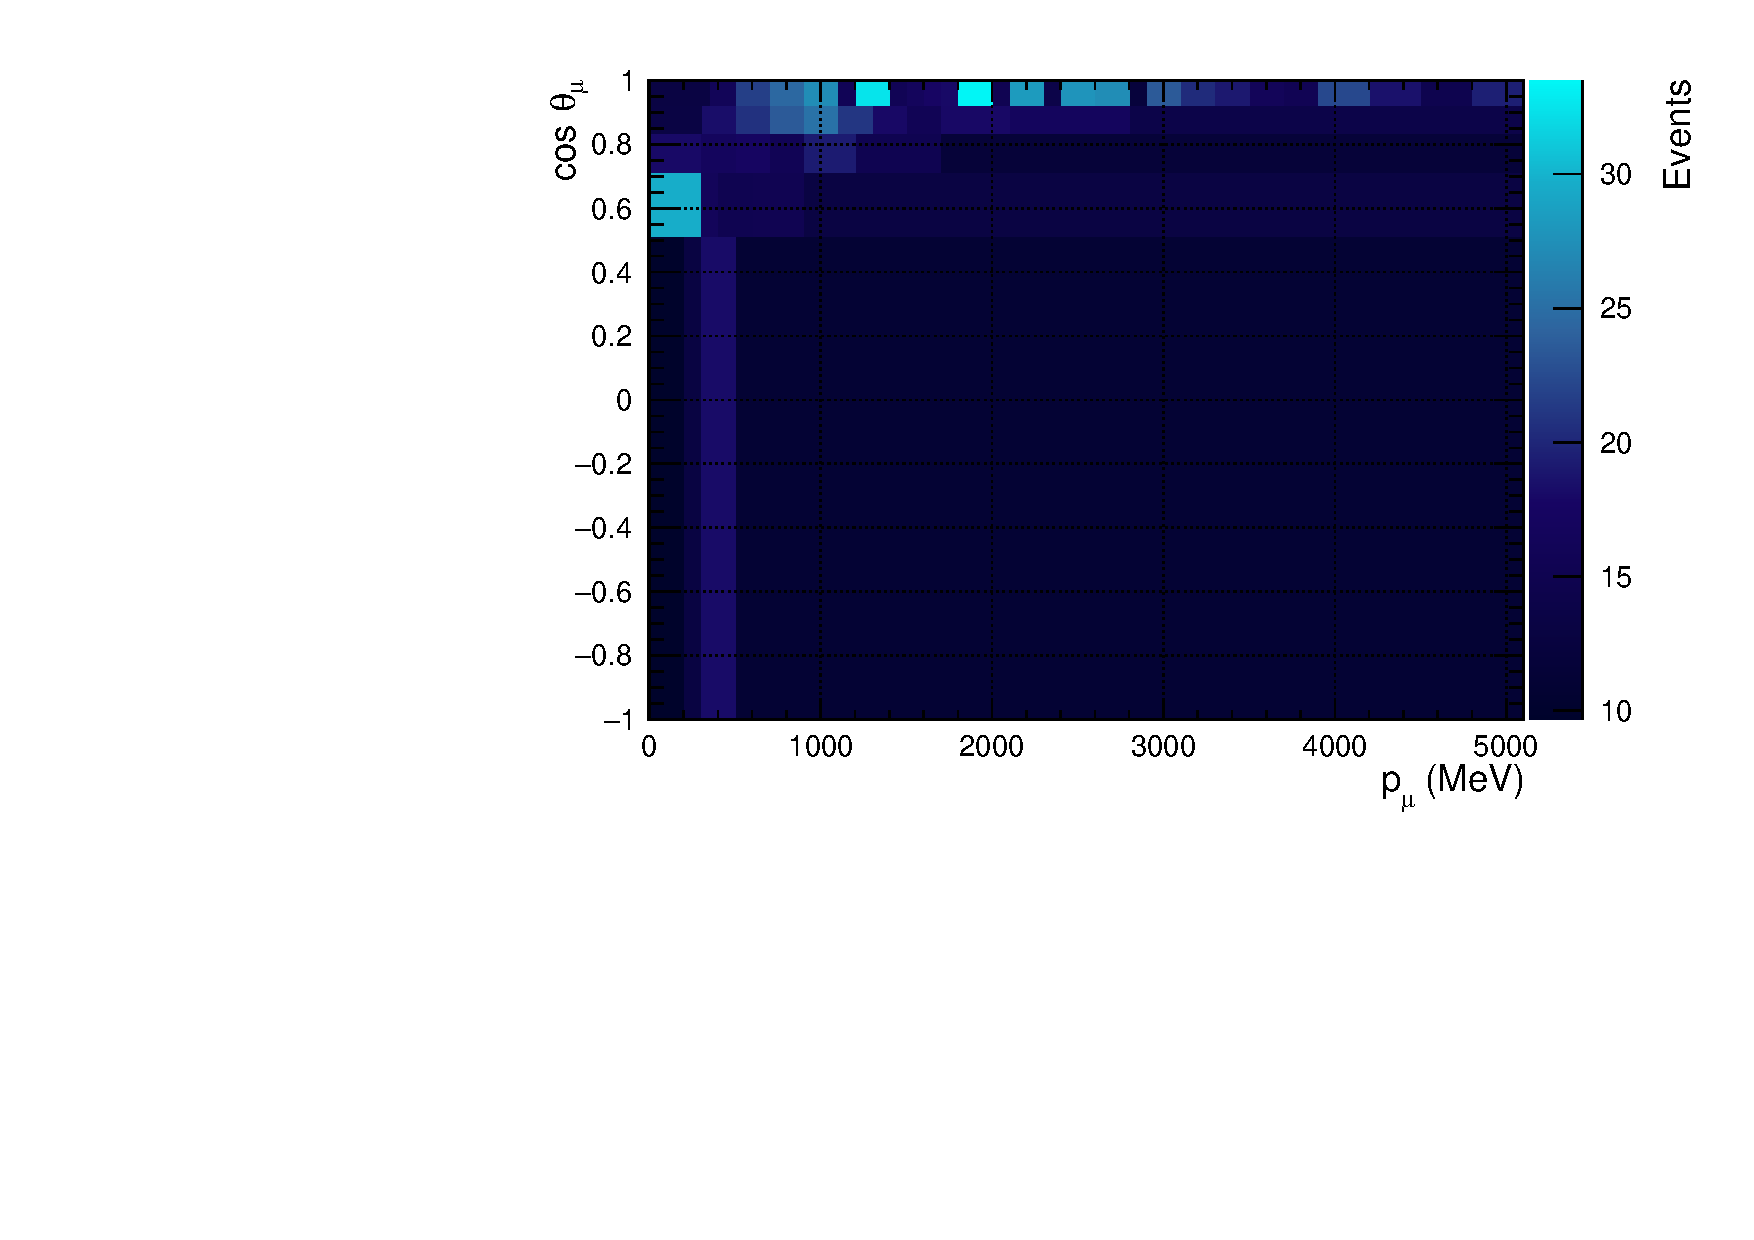
\includegraphics[width=0.95\linewidth]{figs/TH2PolyNom_MC_FGD1_NuMuBkg_CC1pi_in_AntiNu_Mode}
  \caption{FGD1 RHC $\nu_{\mu}$ 1$\pi$}
  \label{fig:th2polynomFGD1_NuMuBkg_CC1pi_in_AntiNu_Mode}
\end{subfigure}
\begin{subfigure}{.32\textwidth}
  \centering
  \includegraphics[width=0.95\linewidth]{figs/TH2PolyNom_MC_FGD1_NuMuBkg_CCOther_in_AntiNu_Mode}
  \caption{FGD1 RHC $\nu_{\mu}$ Other}
  \label{fig:th2polynomFGD1_NuMuBkg_CCOther_in_AntiNu_Mode}
\end{subfigure}
\begin{subfigure}{.32\textwidth}
  \centering
  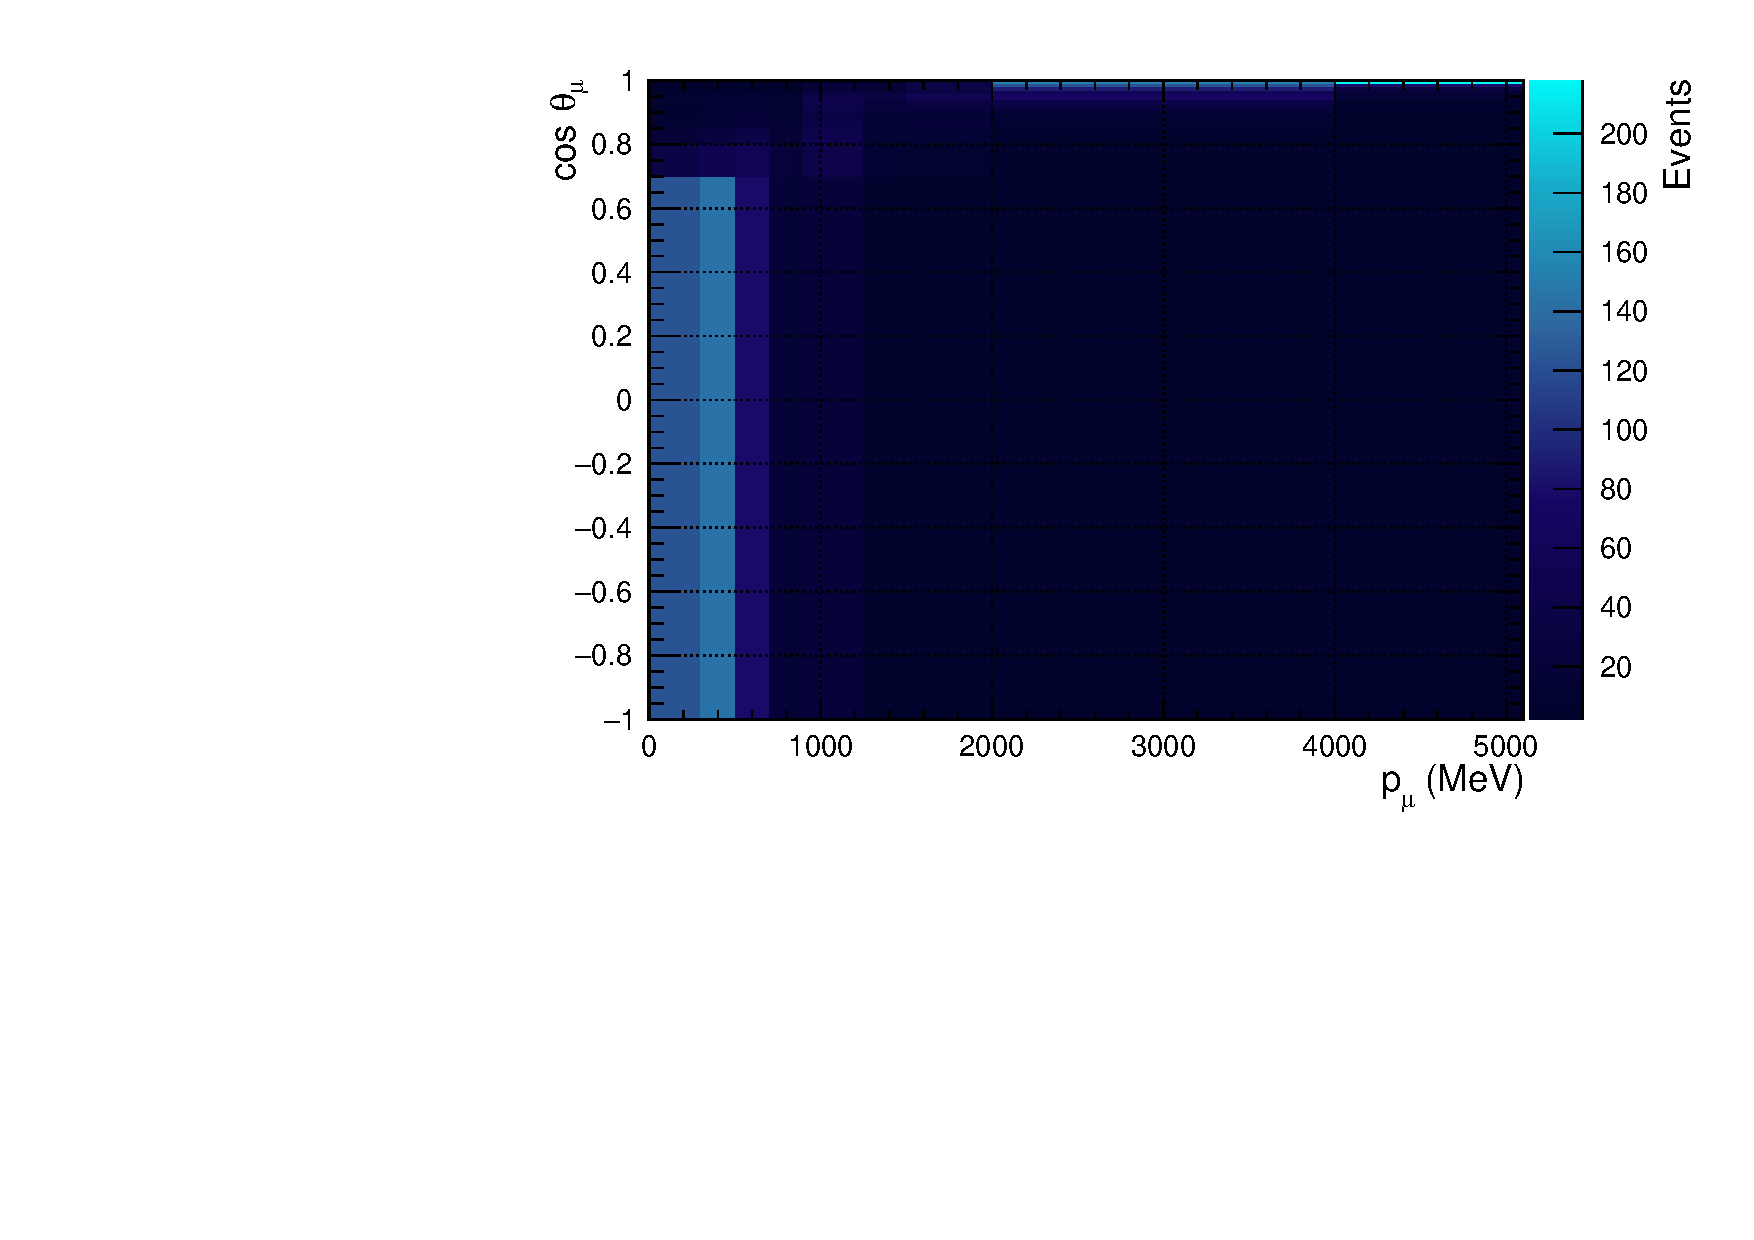
\includegraphics[width=0.95\linewidth]{figs/TH2PolyNom_MC_FGD2_NuMuBkg_CC0pi_in_AntiNu_Mode}
  \caption{FGD2 RHC $\nu_{\mu}$ 0$\pi$}
  \label{fig:th2polynomFGD2_NuMuBkg_CC0pi_in_AntiNu_Mode}
\end{subfigure}
\begin{subfigure}{.32\textwidth}
  \centering
  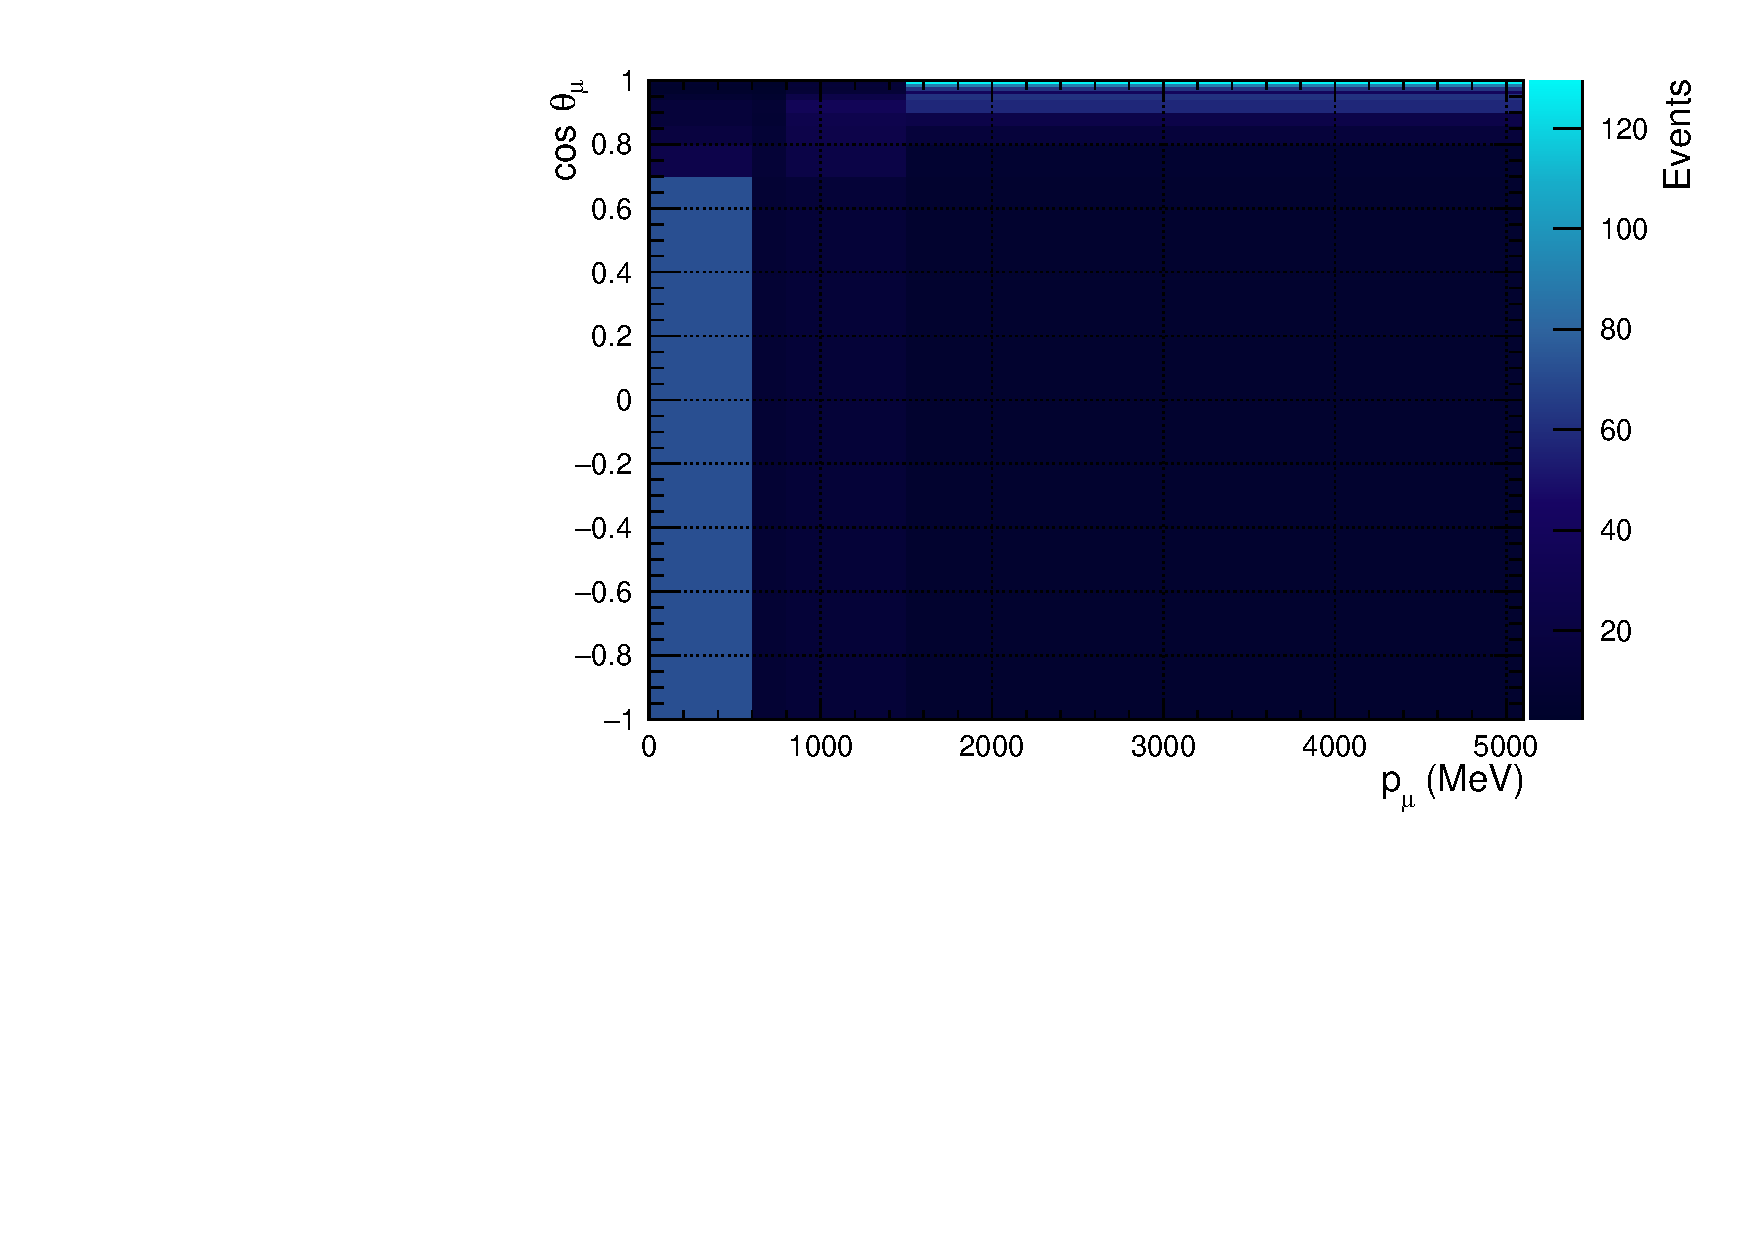
\includegraphics[width=0.95\linewidth]{figs/TH2PolyNom_MC_FGD2_NuMuBkg_CC1pi_in_AntiNu_Mode}
  \caption{FGD2 RHC $\nu_{\mu}$ 1$\pi$}
  \label{fig:th2polynomFGD2_NuMuBkg_CC1pi_in_AntiNu_Mode}
\end{subfigure}
\begin{subfigure}{.32\textwidth}
  \centering
  \includegraphics[width=0.95\linewidth]{figs/TH2PolyNom_MC_FGD2_NuMuBkg_CCOther_in_AntiNu_Mode}
  \caption{FGD2 RHC $\nu_{\mu}$ Other}
  \label{fig:th2polynomFGD2_NuMuBkg_CCOther_in_AntiNu_Mode}
\end{subfigure}
\caption{$p_{\mu}$--cos $\theta_{\mu}$ distributions for the nominal MC with non-uniform rectangular binning.}
\label{fig:th2polynombin}
\end{figure}

\begin{figure}[!t]
\centering
\begin{subfigure}{.24\textwidth}
  \centering
  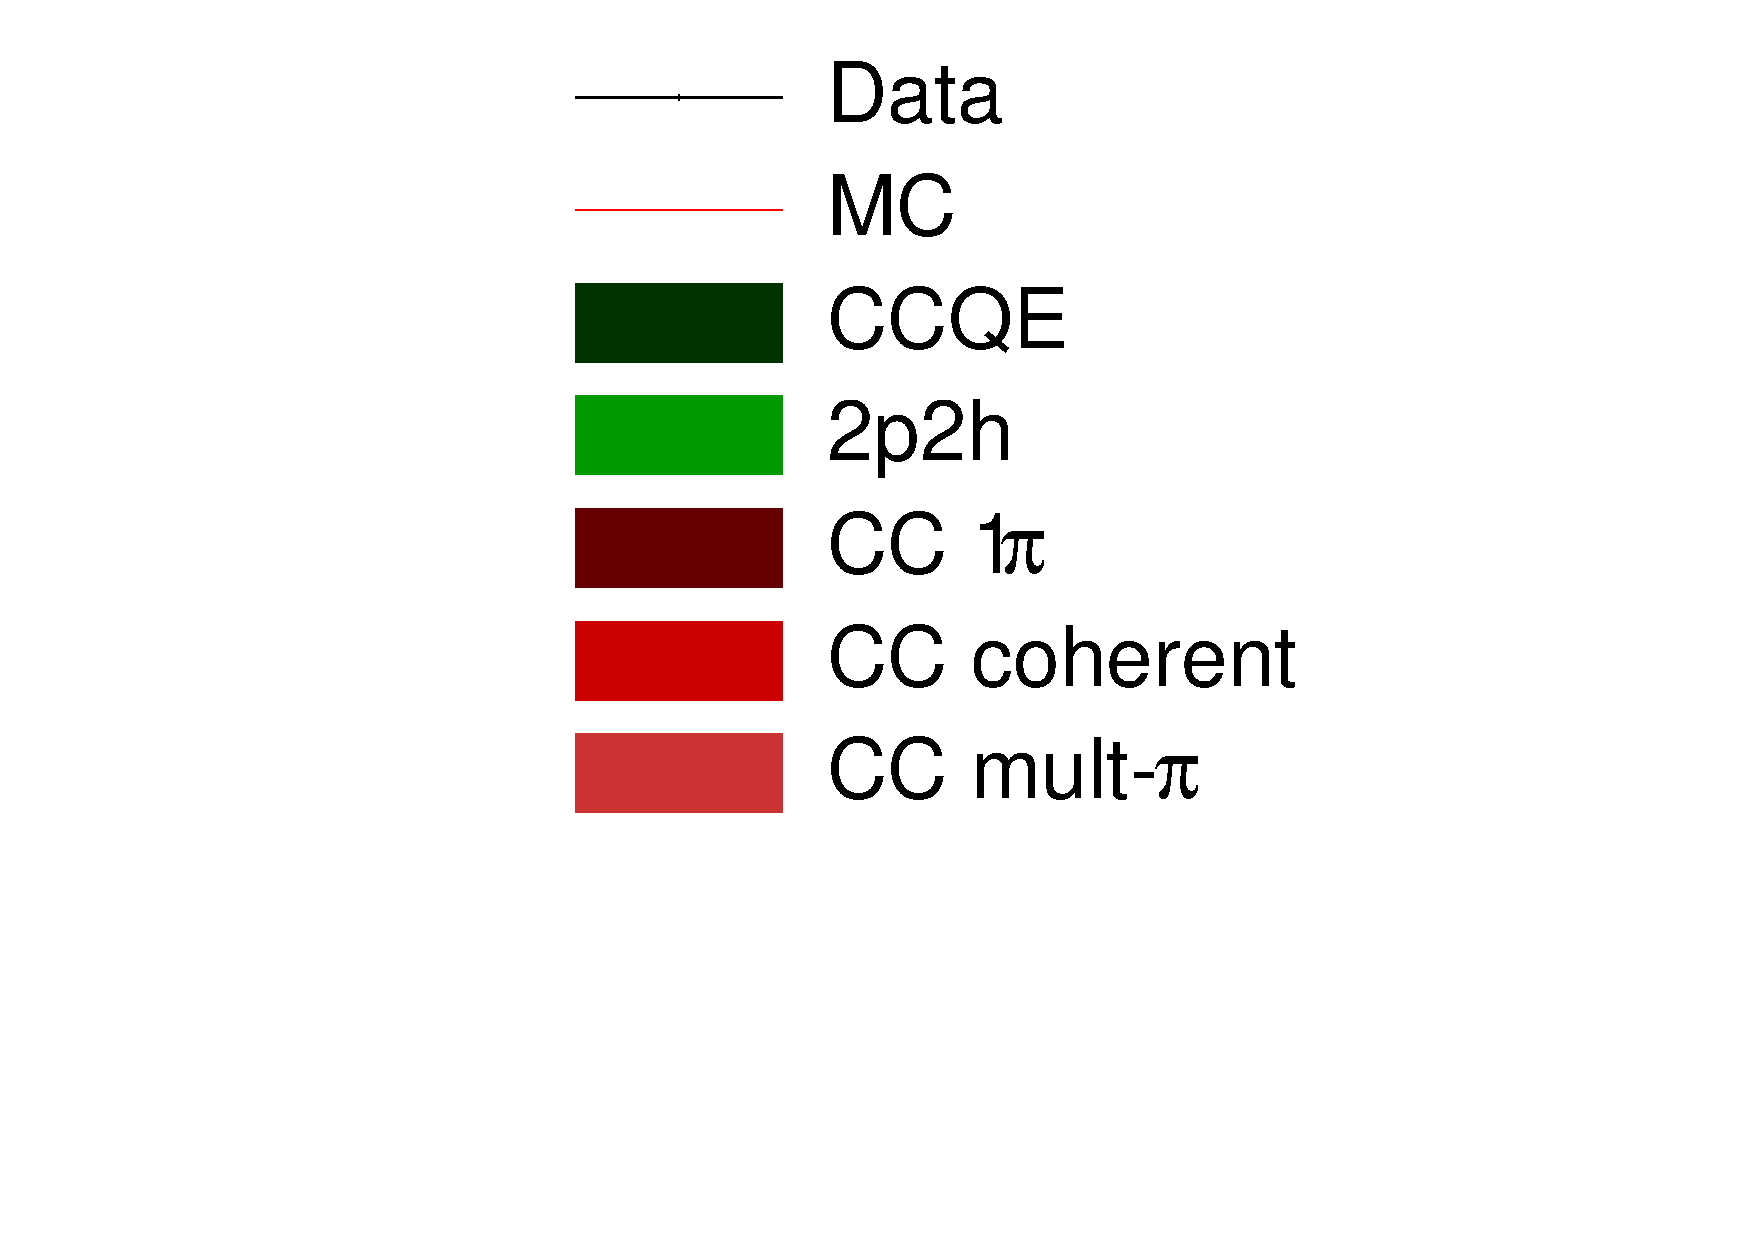
\includegraphics[width=\linewidth, trim={5mm 60mm 30mm 0mm}, clip]{figs/legend}
\end{subfigure}
\begin{subfigure}{.24\textwidth}
  \centering
  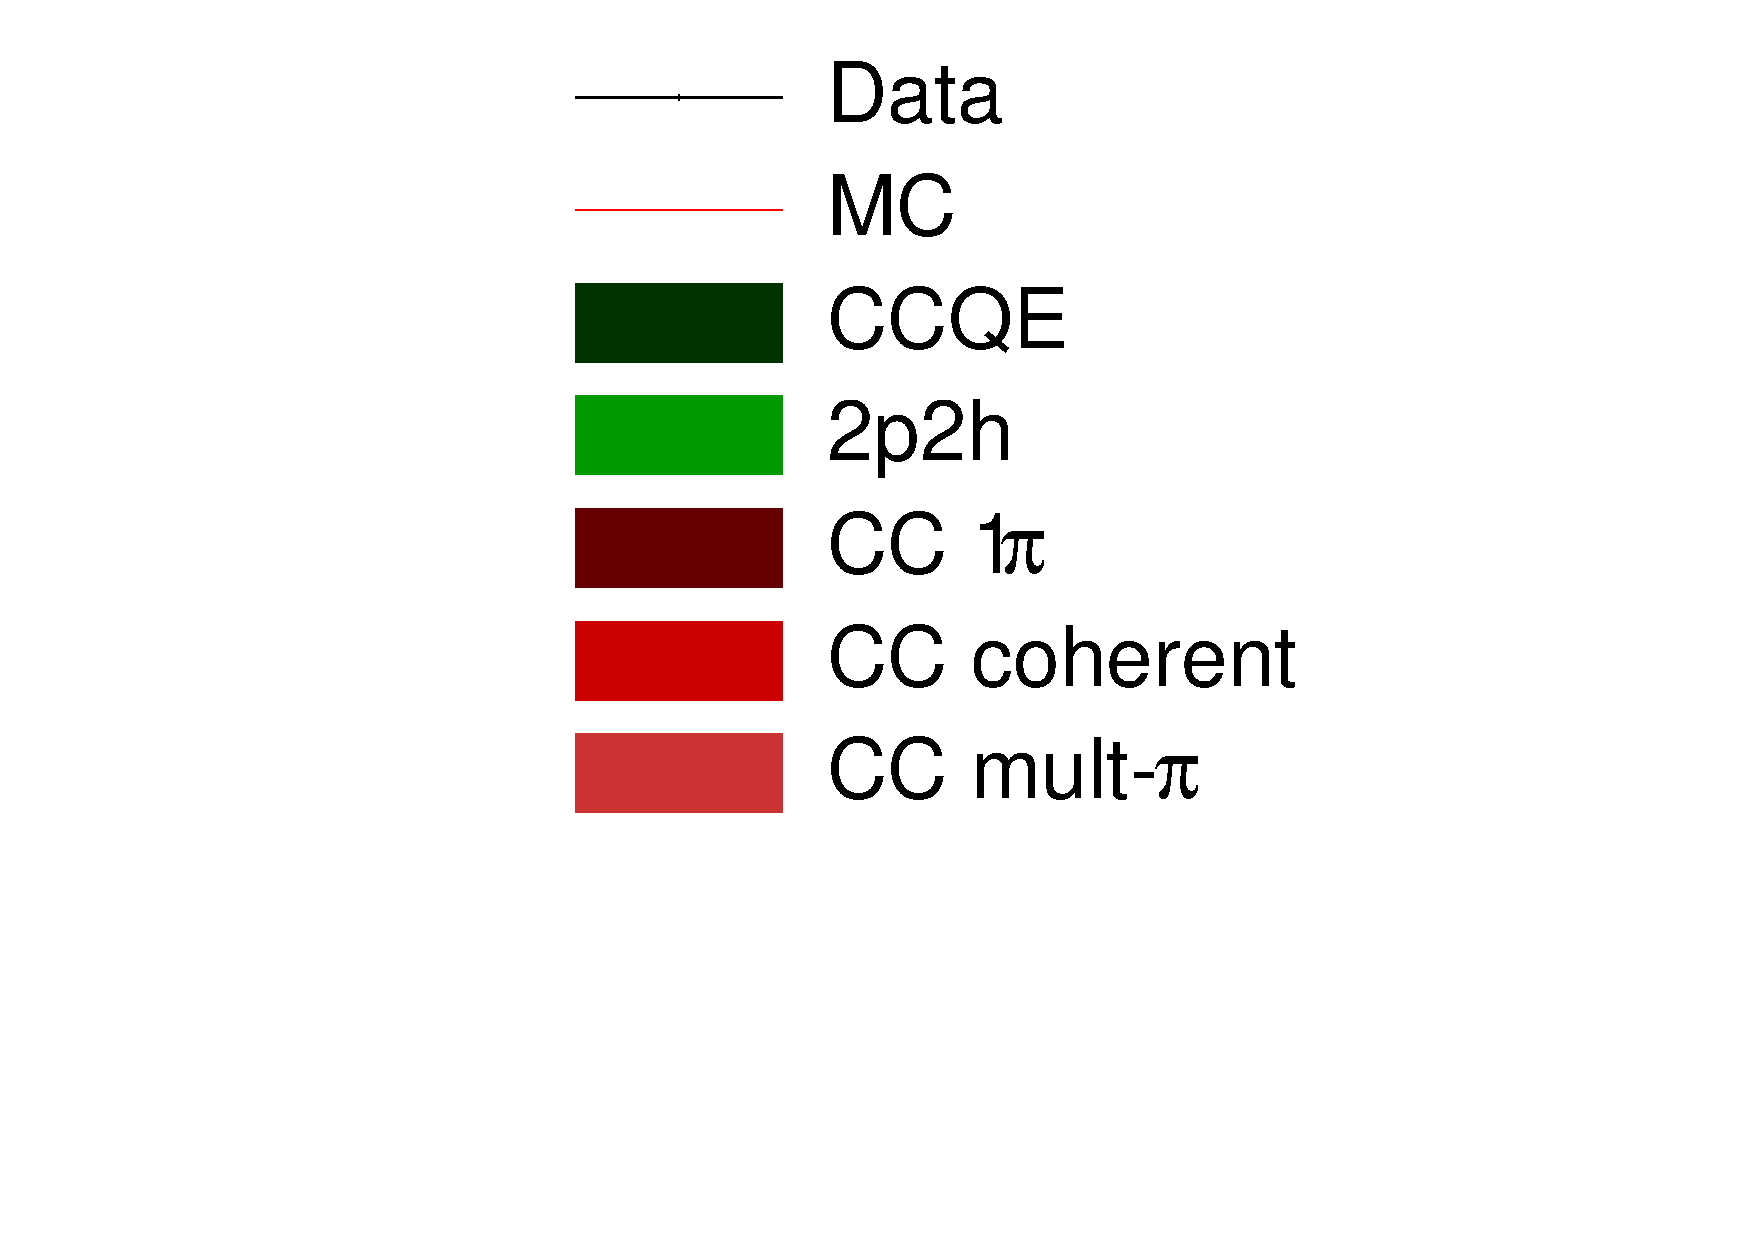
\includegraphics[width=\linewidth, trim={5mm 0mm 30mm 80mm}, clip]{figs/legend}
\end{subfigure}
\begin{subfigure}{.24\textwidth}
  \centering
  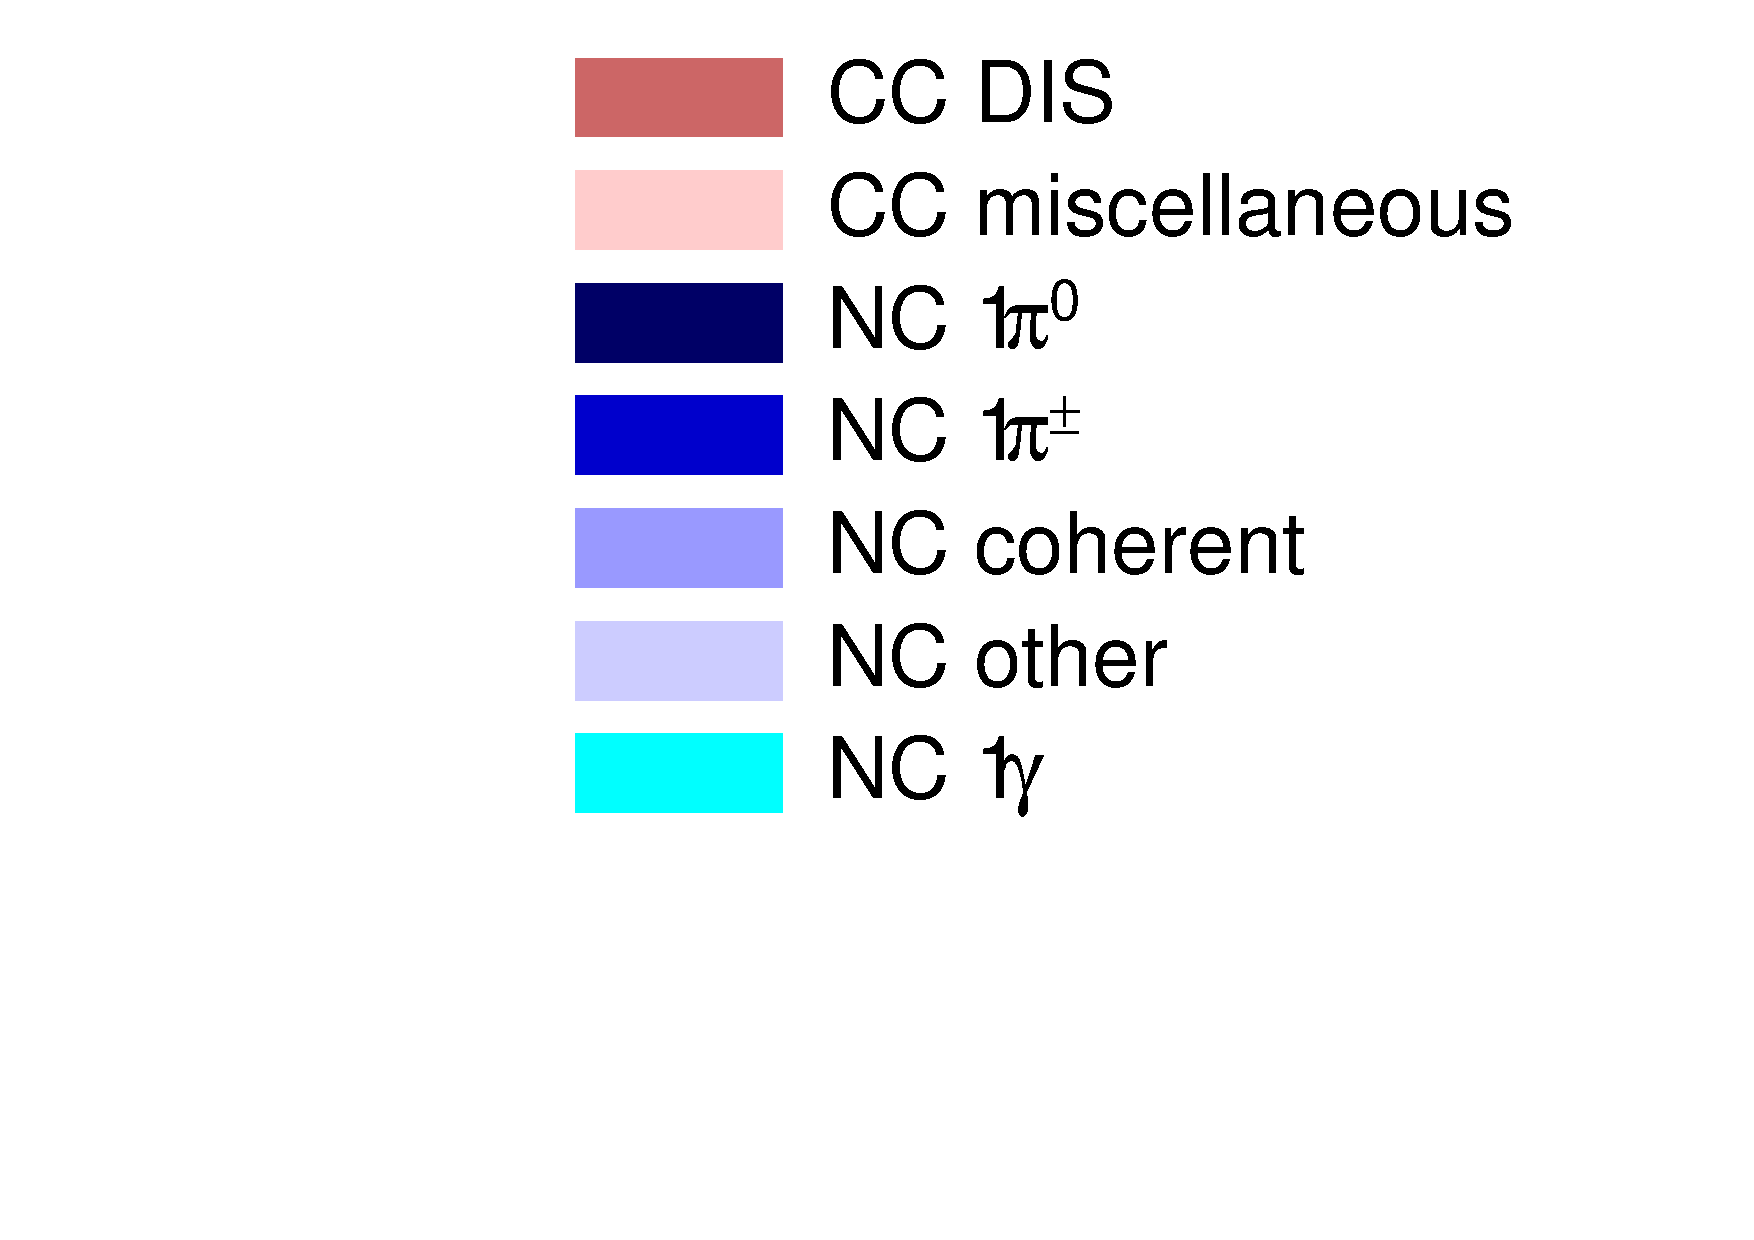
\includegraphics[width=\linewidth, trim={5mm 60mm 30mm 0mm}, clip]{figs/legend2}
\end{subfigure}
\begin{subfigure}{.24\textwidth}
  \centering
  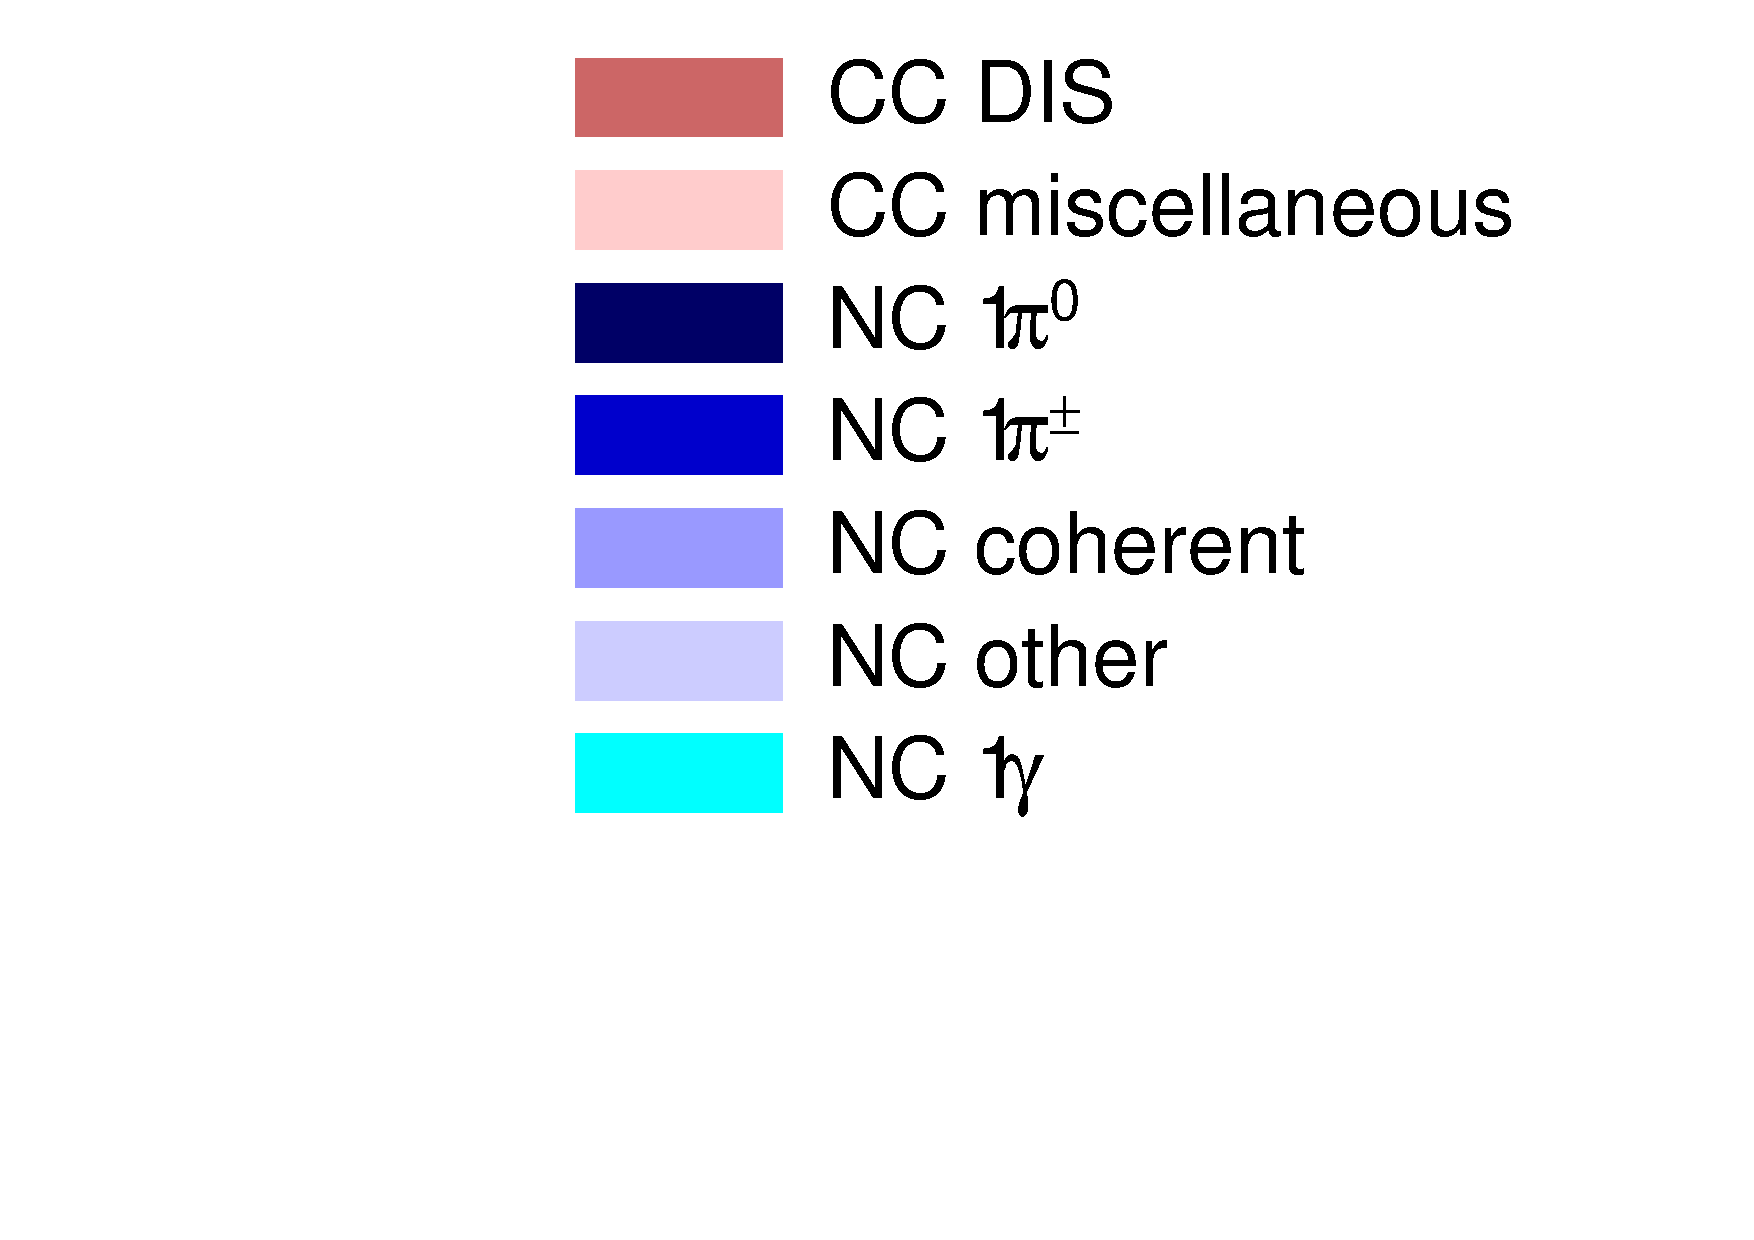
\includegraphics[width=\linewidth, trim={5mm 0mm 30mm 80mm}, clip]{figs/legend2}
\end{subfigure}

\begin{subfigure}{0.49\textwidth}
  \centering
  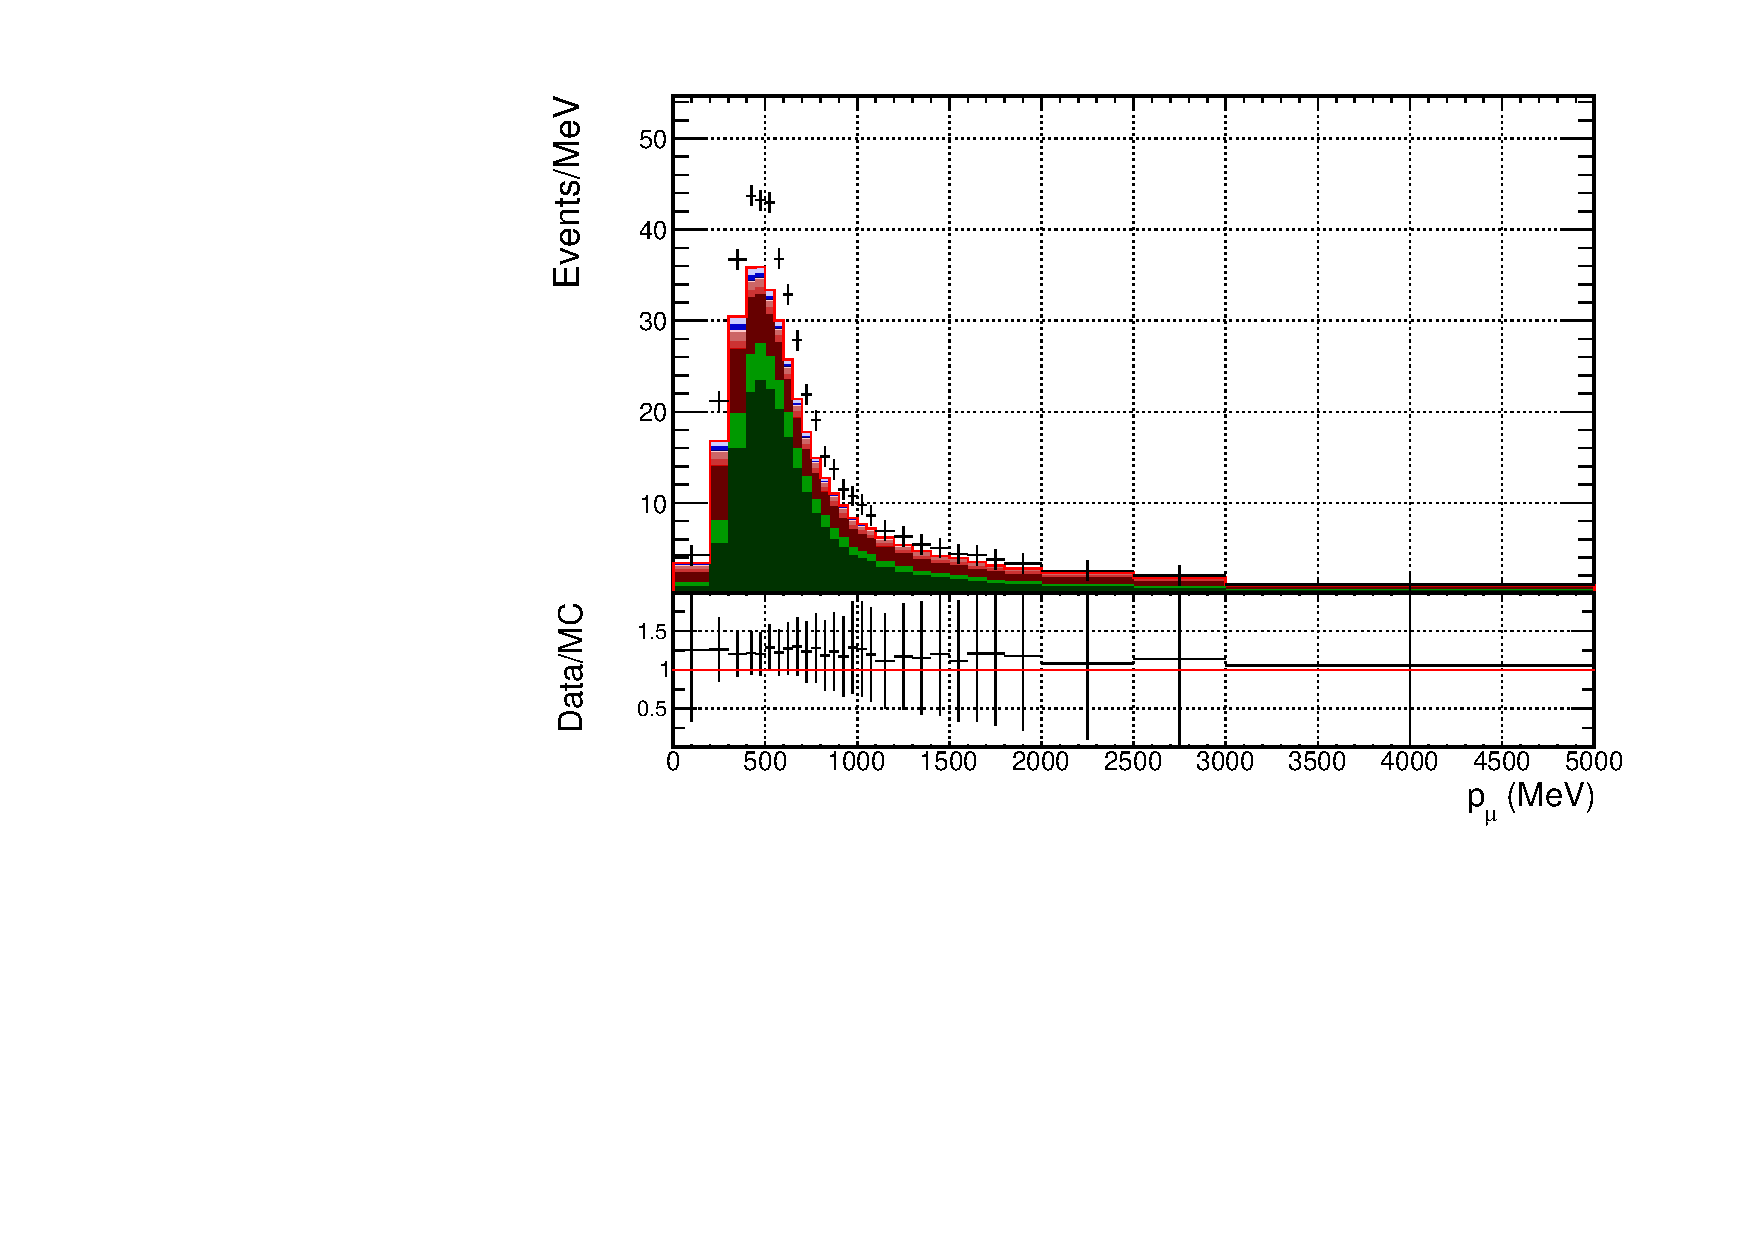
\includegraphics[width=\textwidth]{figs/FGD1_numuCC_0pi_p}
  \caption{FGD1 FHC $\nu_{\mu}$ 0$\pi$}
\end{subfigure}
\begin{subfigure}{0.49\textwidth}
  \centering
  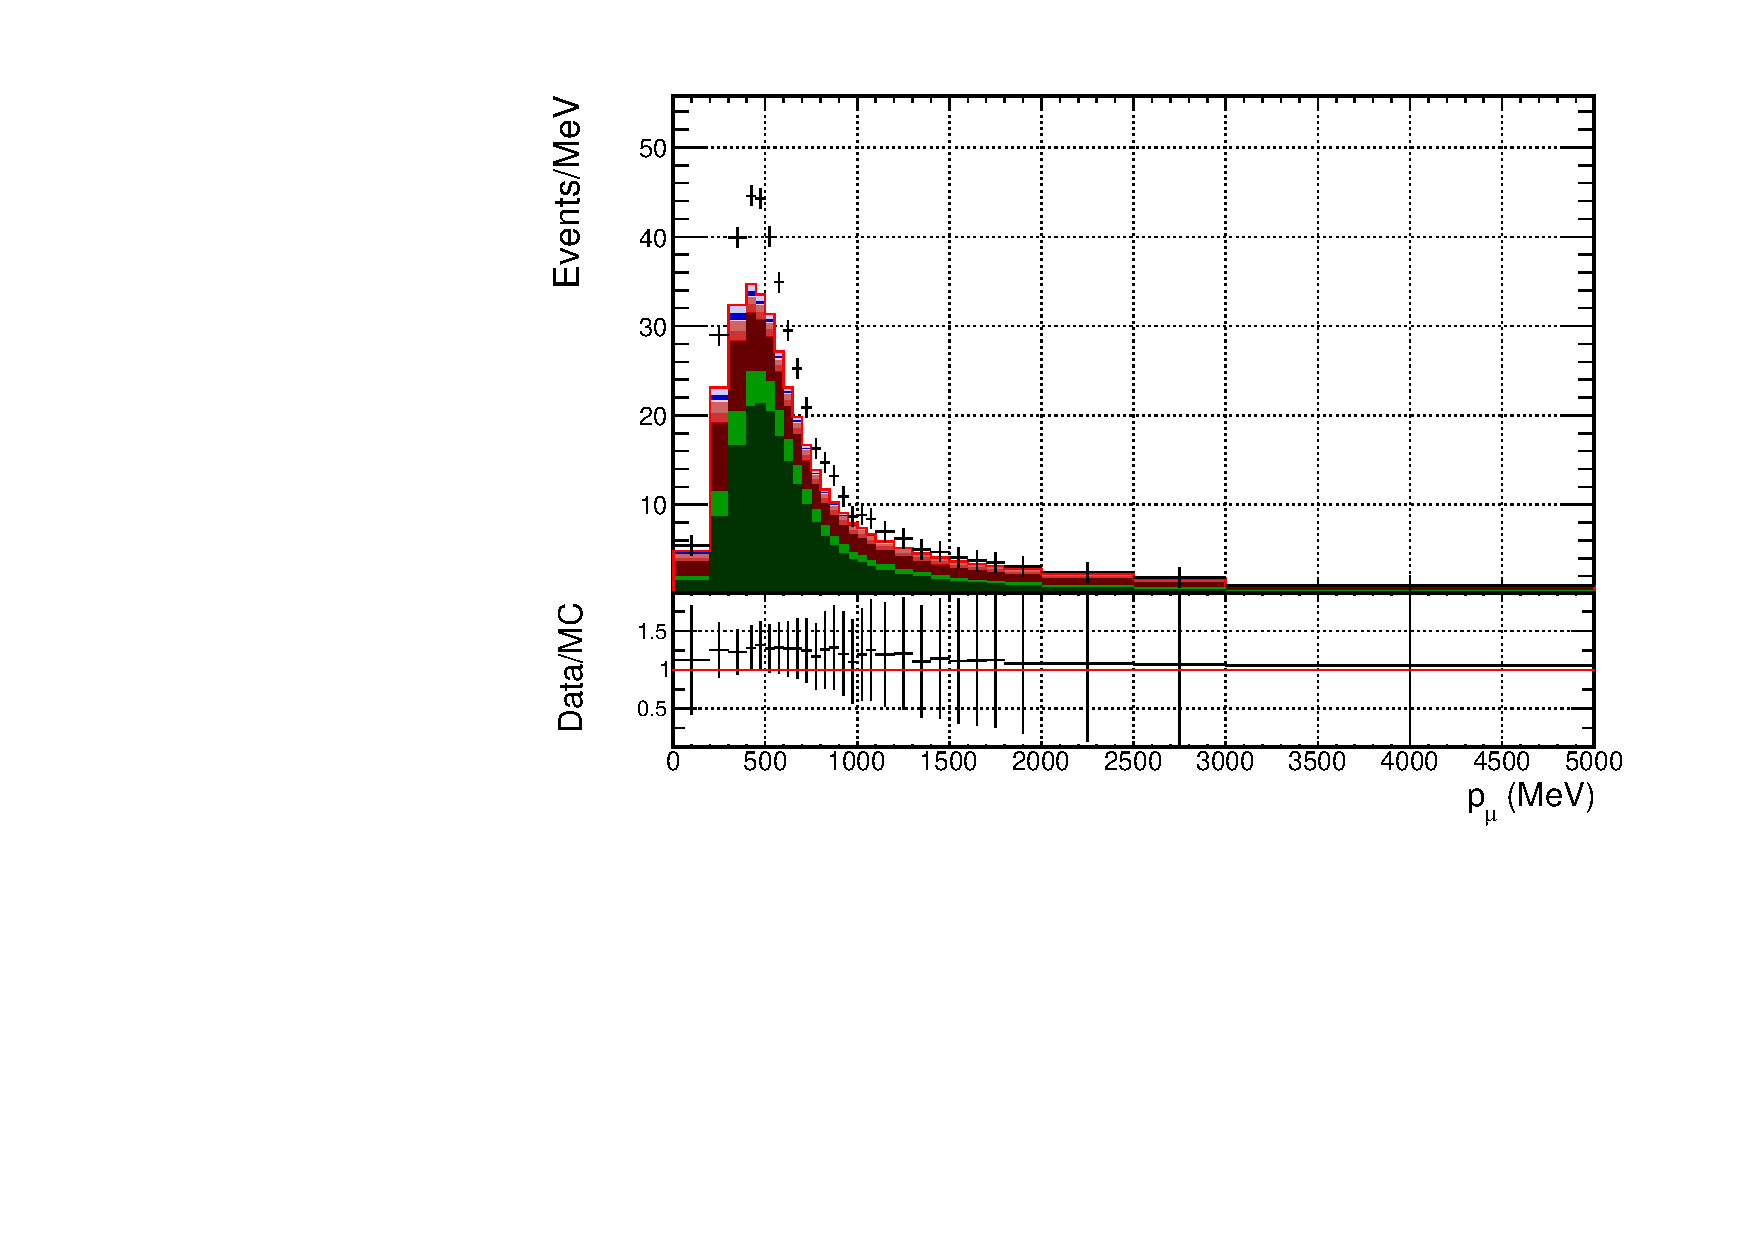
\includegraphics[width=\textwidth]{figs/FGD2_numuCC_0pi_p}
  \caption{FGD2 FHC $\nu_{\mu}$ 0$\pi$}
\end{subfigure}

\begin{subfigure}{0.49\textwidth}
  \centering
  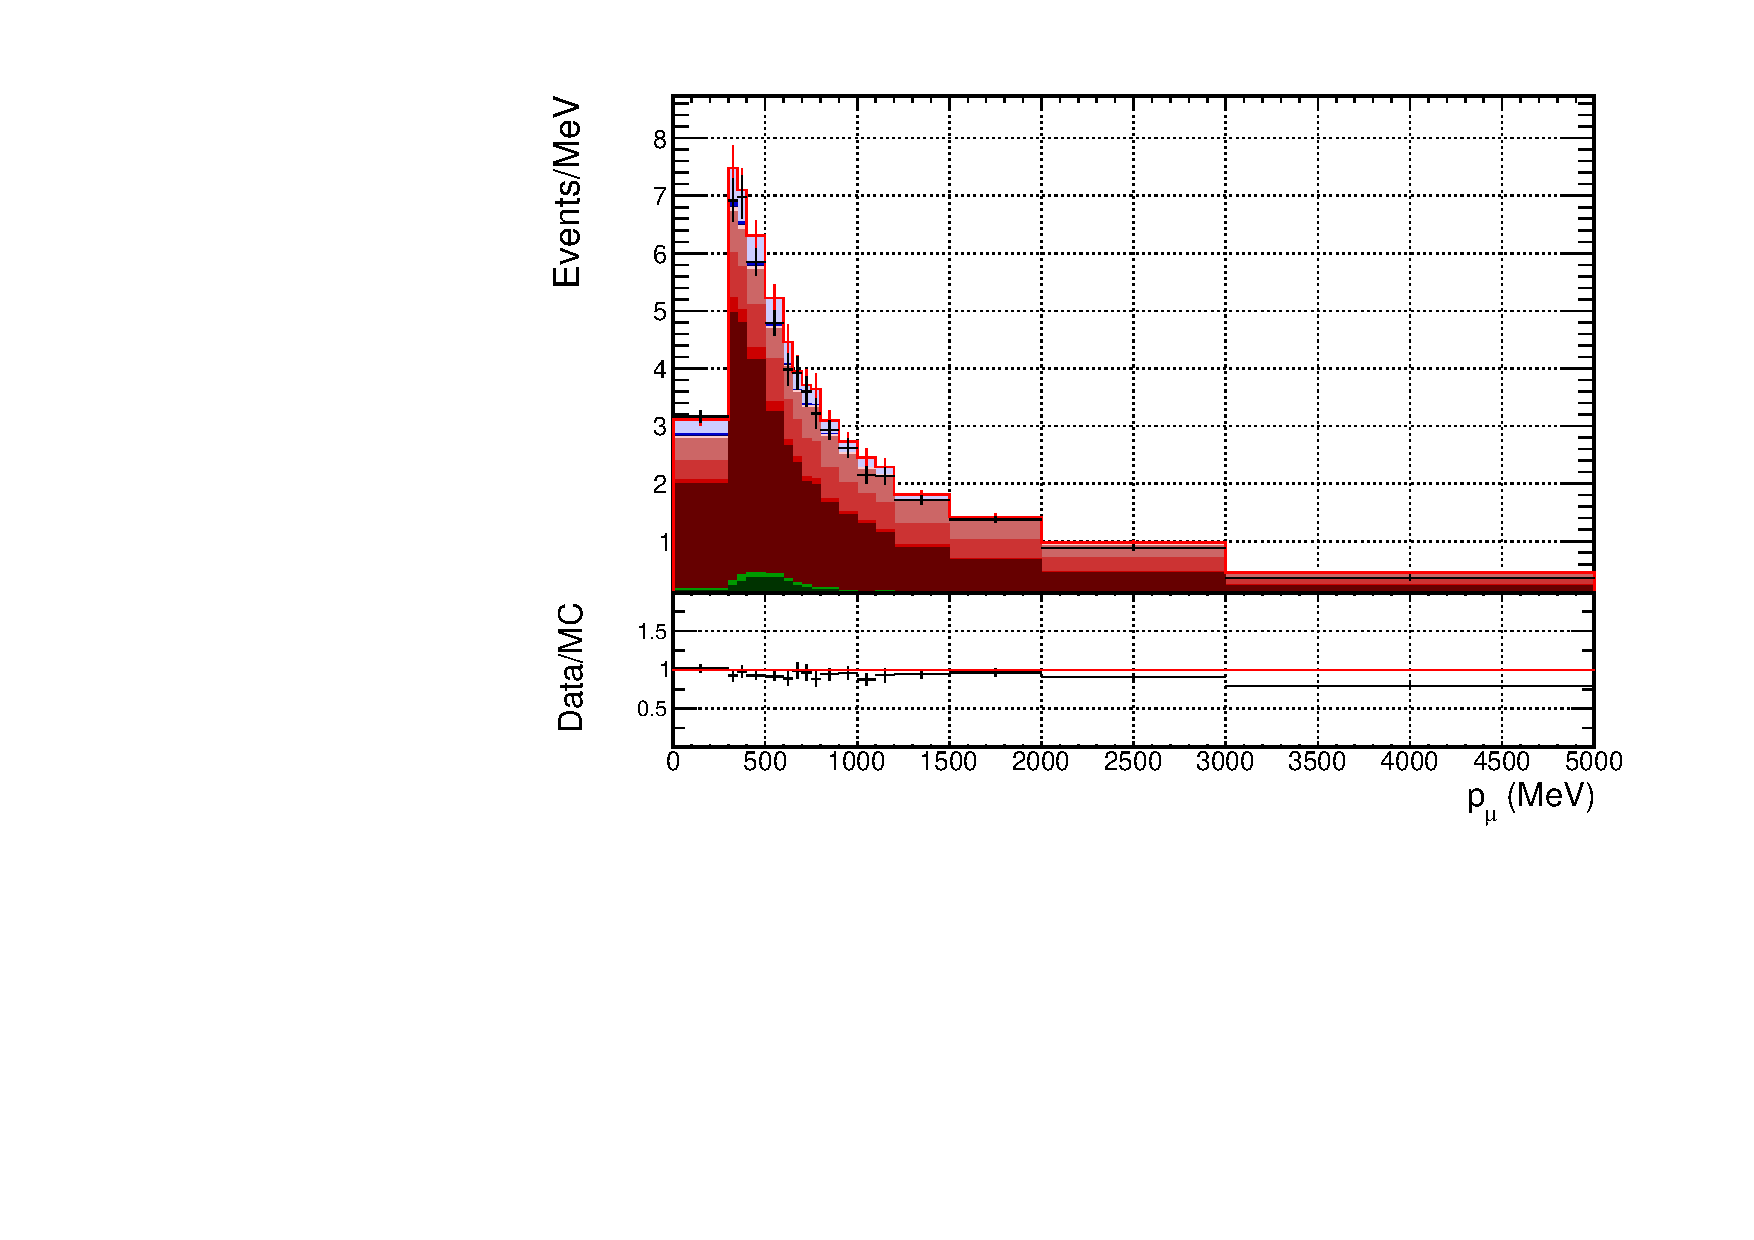
\includegraphics[width=\textwidth]{figs/FGD1_numuCC_1pi_p}
  \caption{FGD1 FHC $\nu_{\mu}$ 1$\pi$}
\end{subfigure}
\begin{subfigure}{0.49\textwidth}
  \centering
  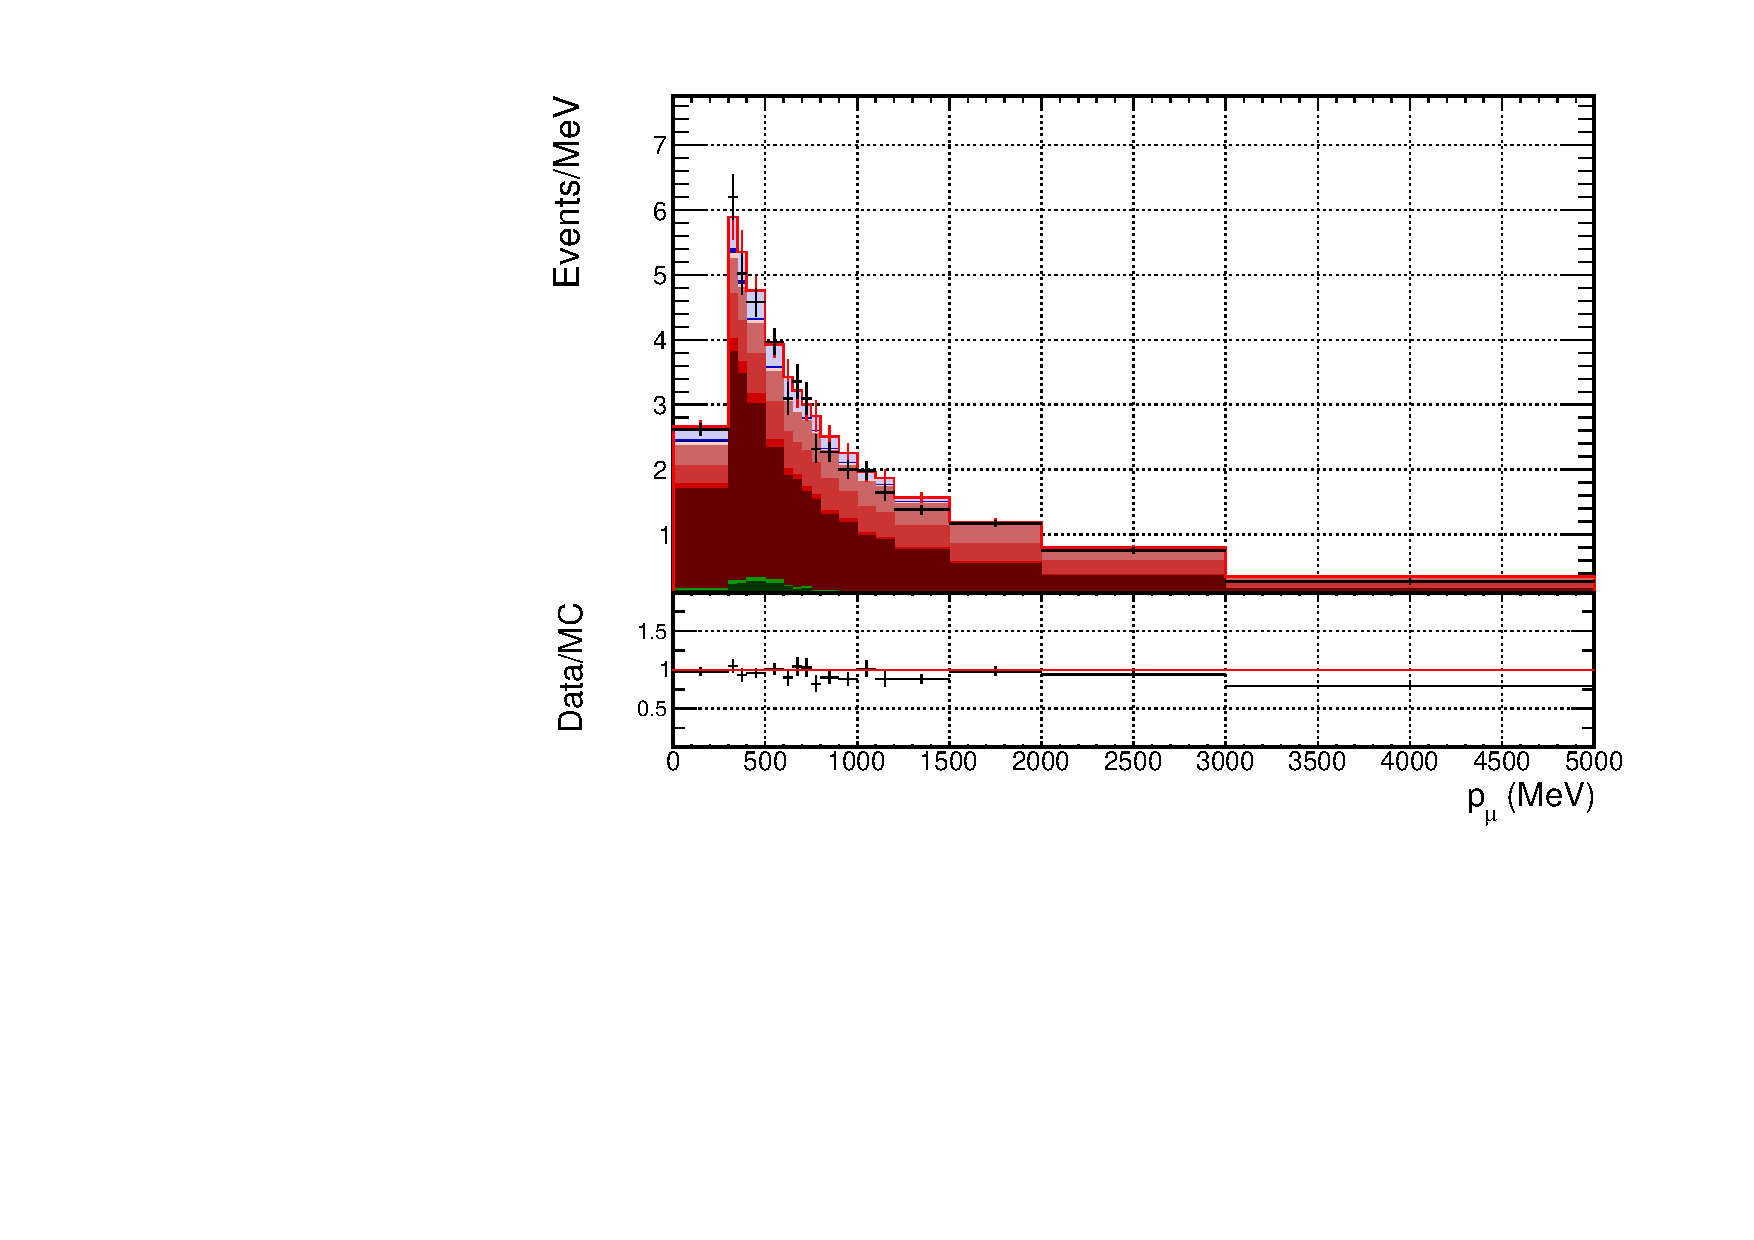
\includegraphics[width=\textwidth]{figs/FGD2_numuCC_1pi_p}
  \caption{FGD2 FHC $\nu_{\mu}$ 1$\pi$}
\end{subfigure}

\begin{subfigure}{0.49\textwidth}
  \centering
  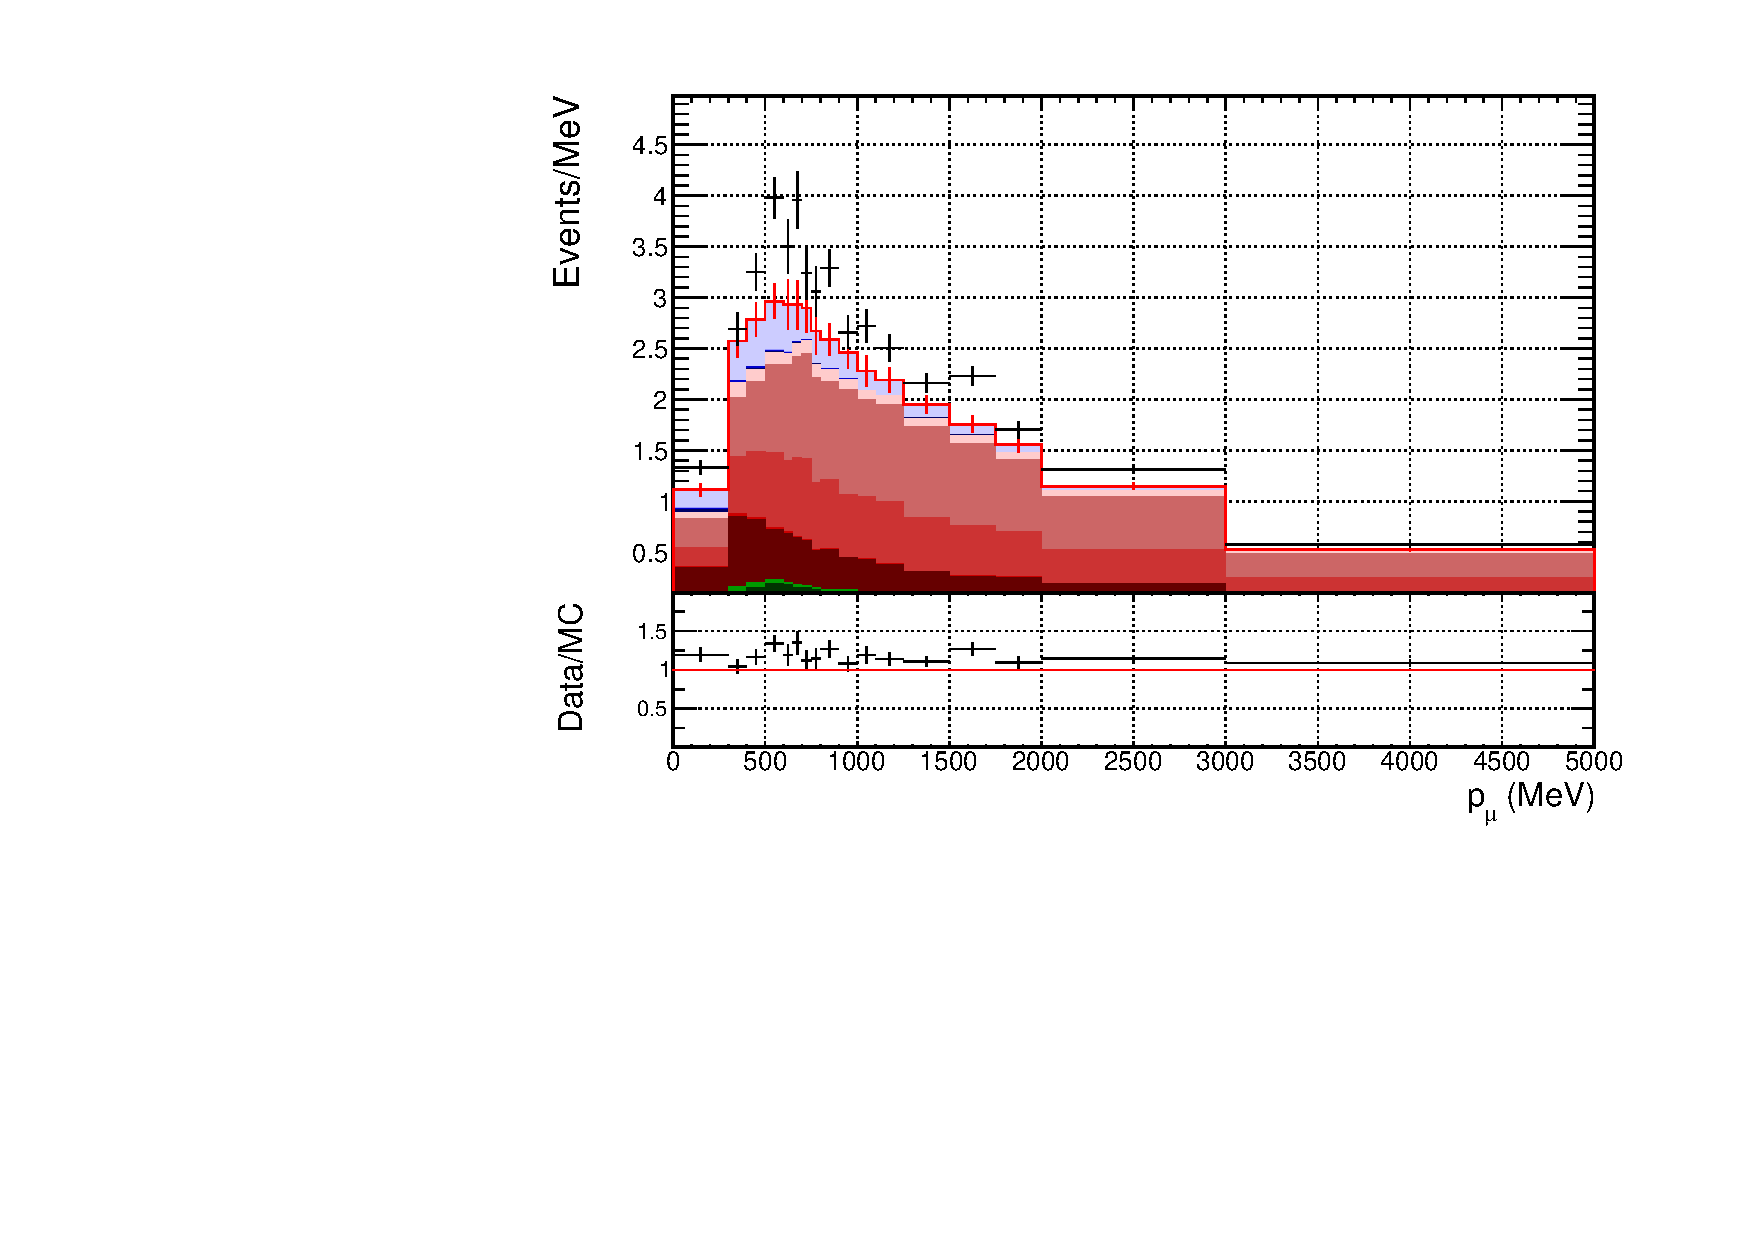
\includegraphics[width=\textwidth]{figs/FGD1_numuCC_other_p}
  \caption{FGD1 FHC $\nu_{\mu}$ Other}
\end{subfigure}
\begin{subfigure}{0.49\textwidth}
  \centering
  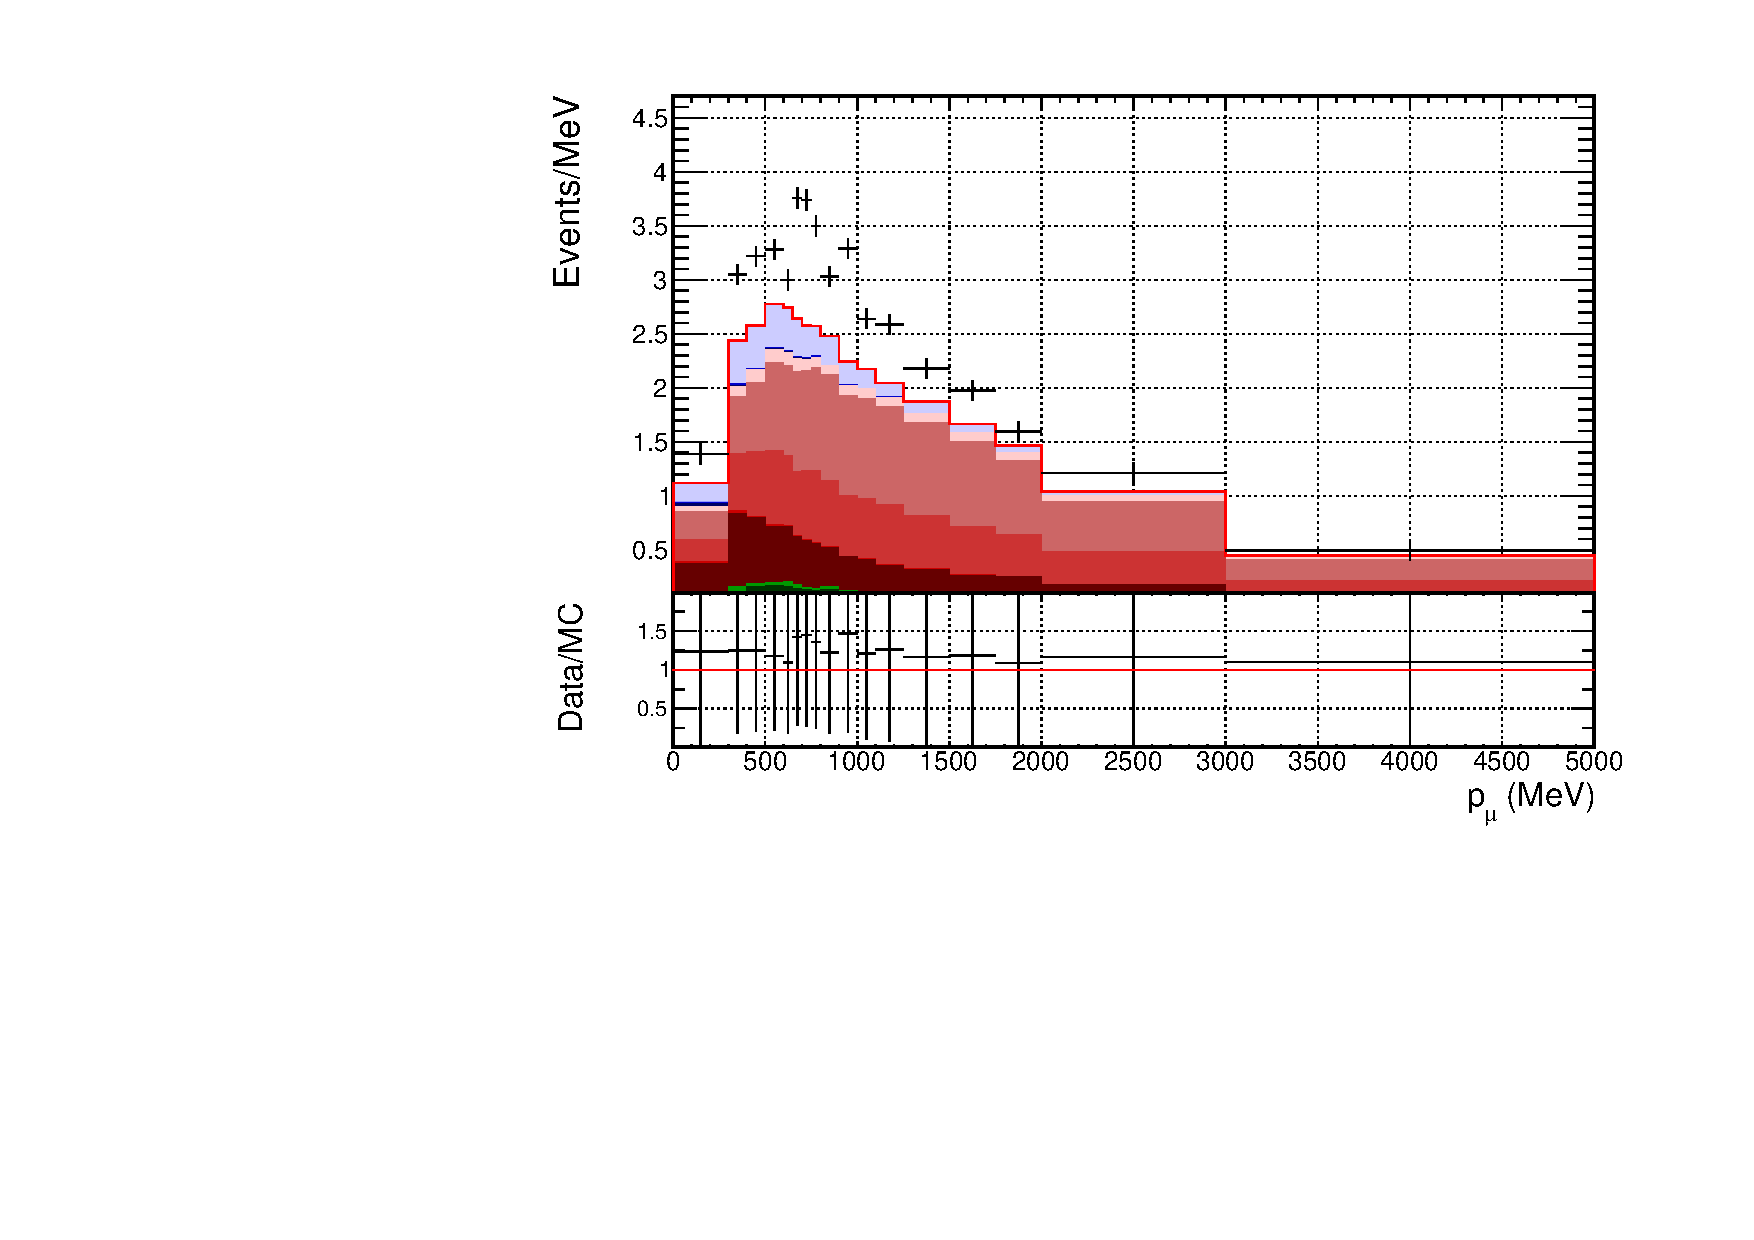
\includegraphics[width=\textwidth]{figs/FGD2_numuCC_other_p}
  \caption{FGD2 FHC $\nu_{\mu}$ Other}
\end{subfigure}
\caption{$p_{\mu}$ projections of data and nominal MC broken down by interaction mode for FHC selections.}
\label{fig:pstack_fhc}
\end{figure}

\begin{figure}[!htbp]
\centering
\begin{subfigure}{.24\textwidth}
  \centering
  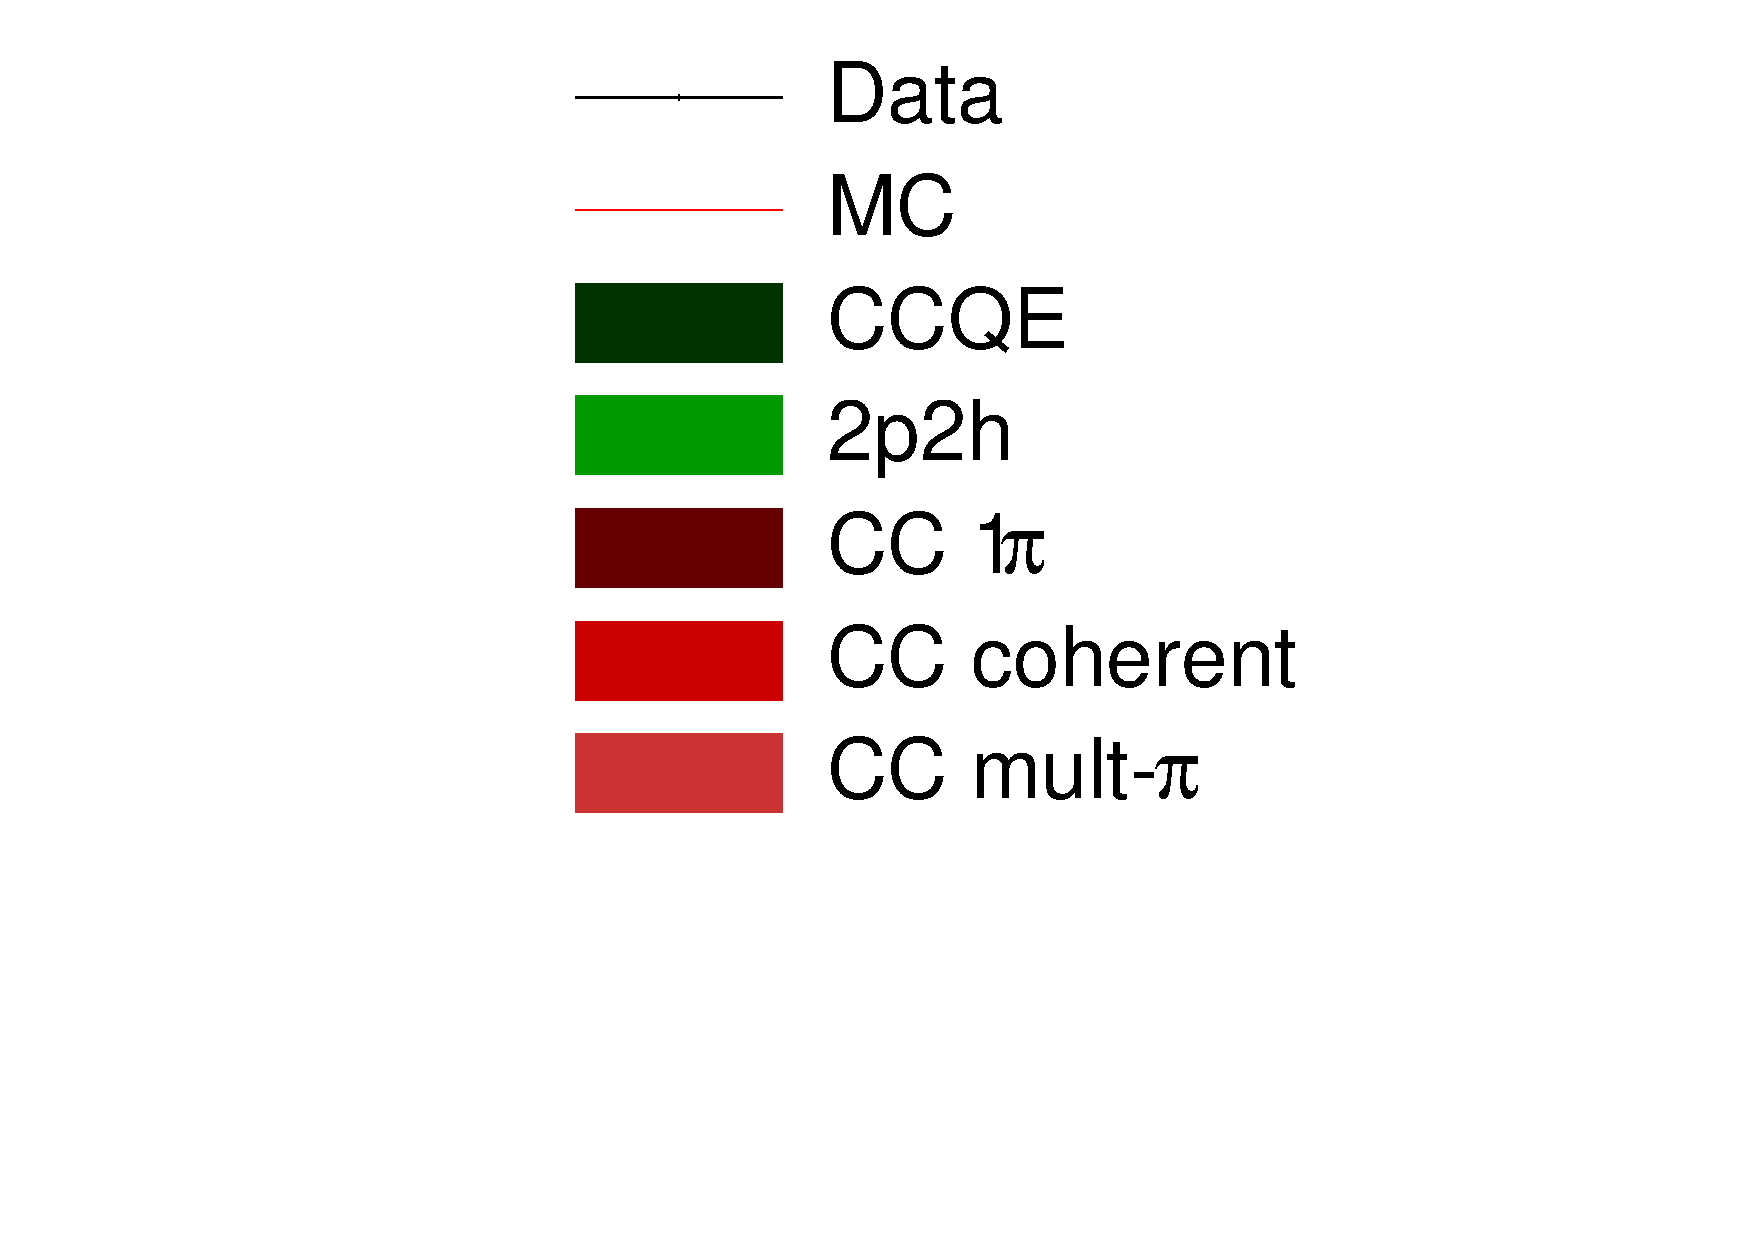
\includegraphics[width=\linewidth, trim={5mm 60mm 30mm 0mm}, clip]{figs/legend}
\end{subfigure}
\begin{subfigure}{.24\textwidth}
  \centering
  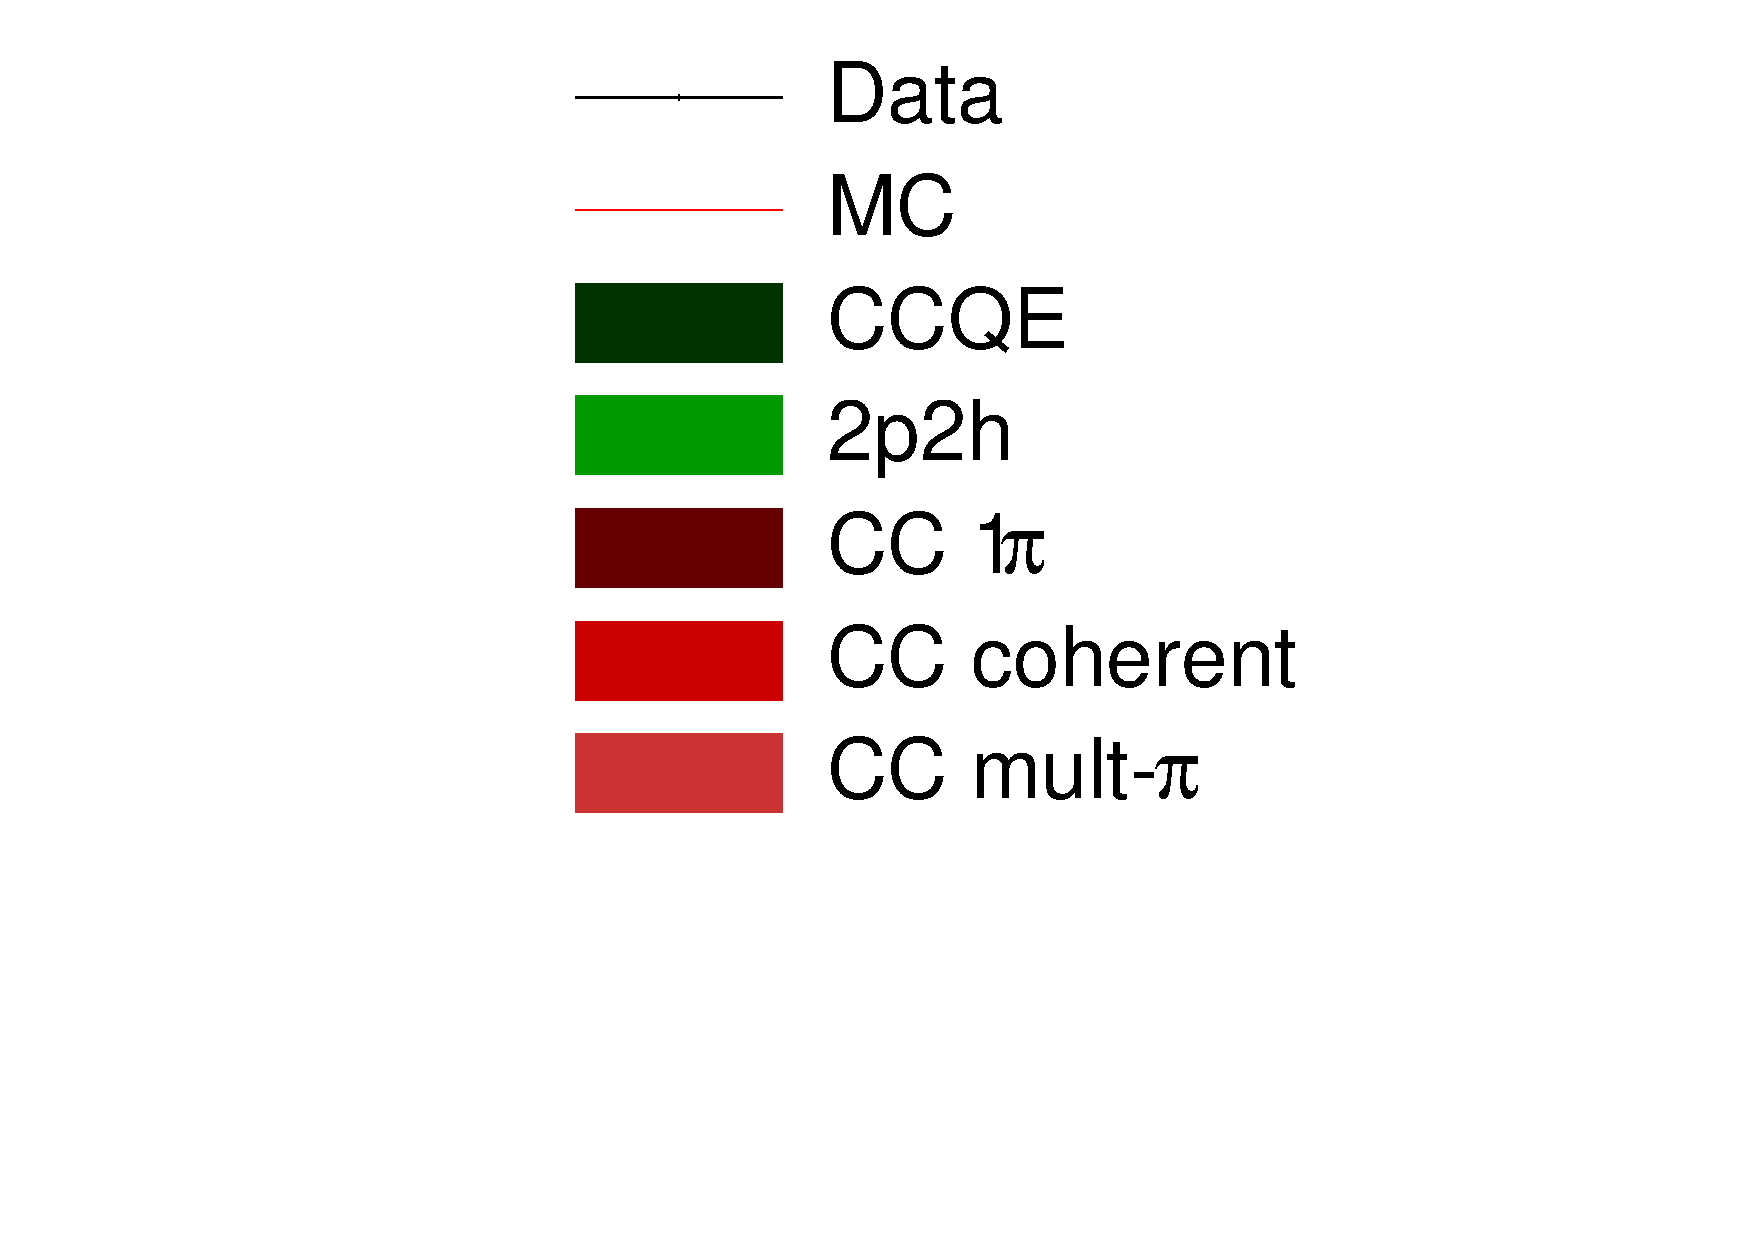
\includegraphics[width=\linewidth, trim={5mm 0mm 30mm 80mm}, clip]{figs/legend}
\end{subfigure}
\begin{subfigure}{.24\textwidth}
  \centering
  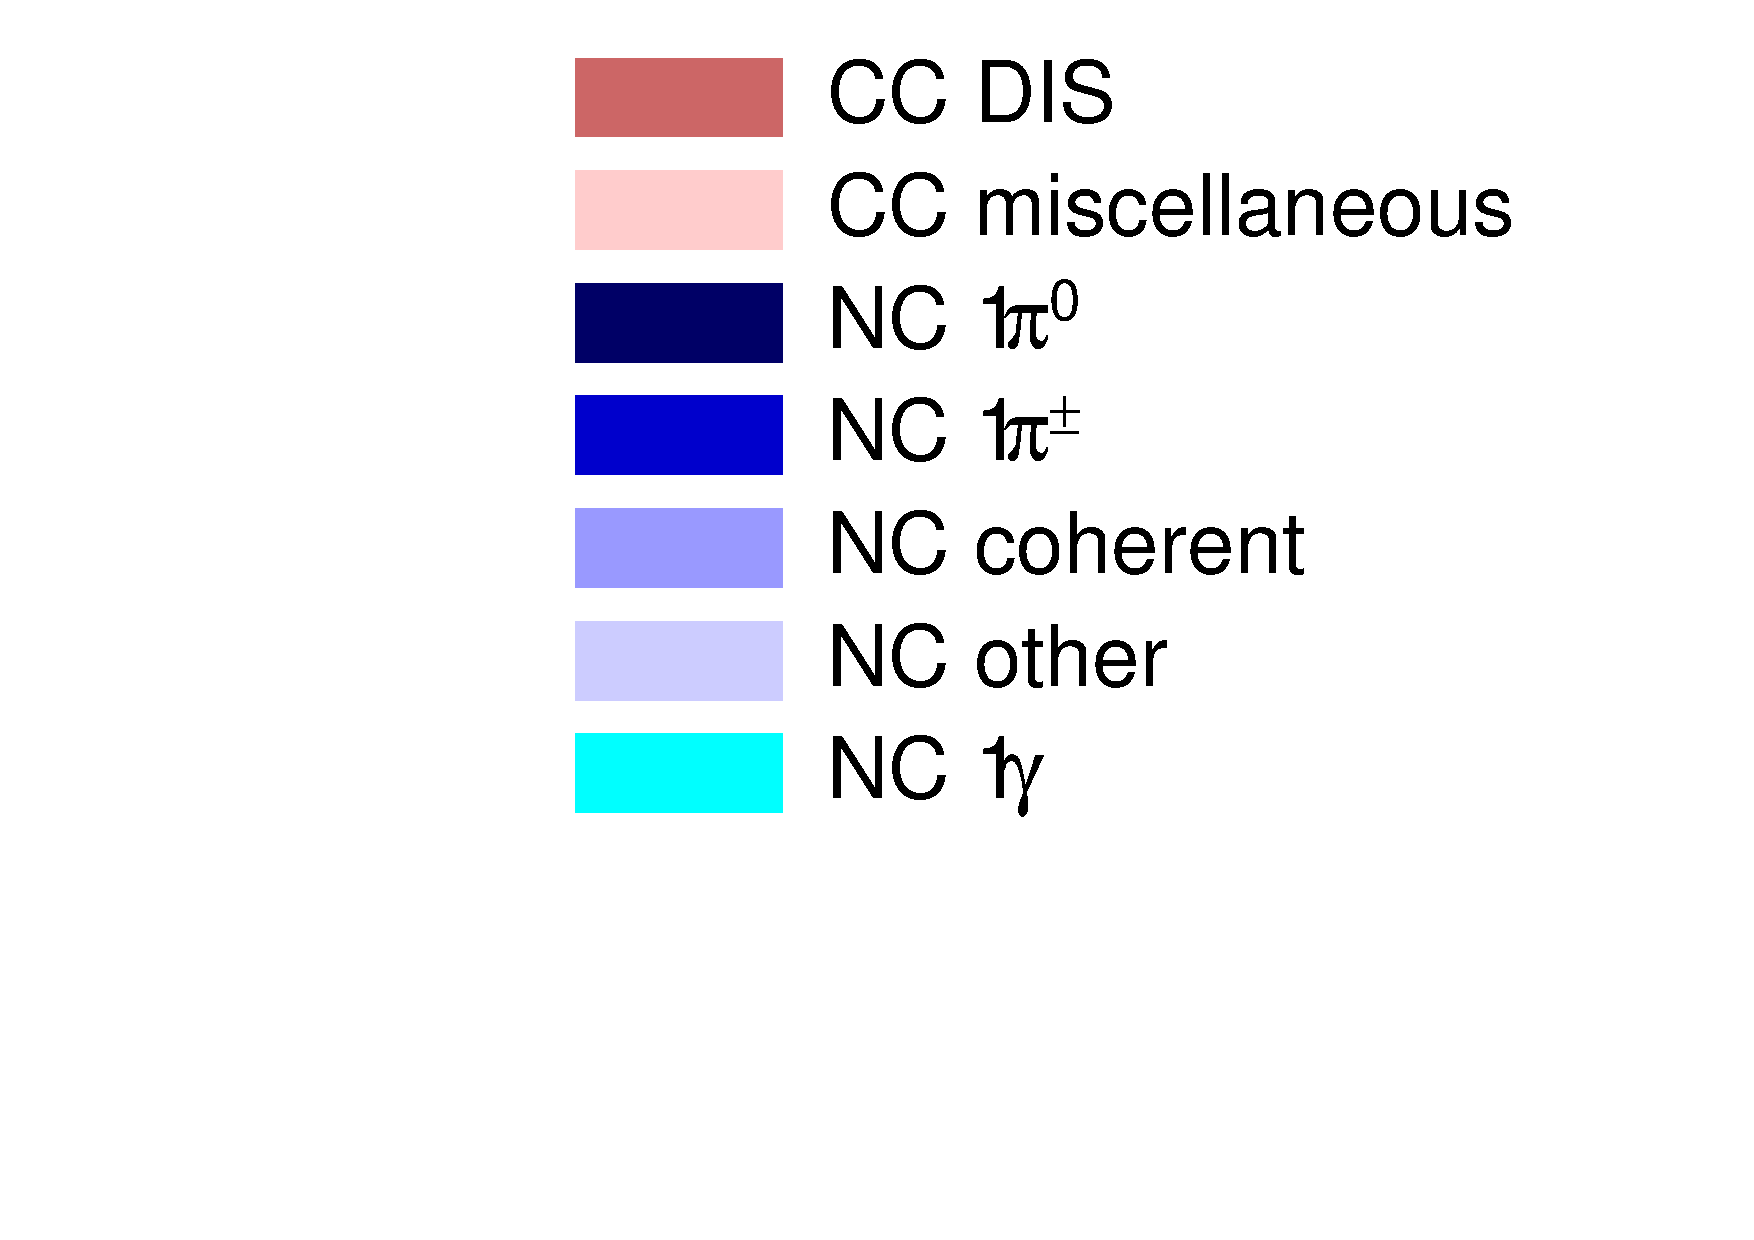
\includegraphics[width=\linewidth, trim={5mm 60mm 30mm 0mm}, clip]{figs/legend2}
\end{subfigure}
\begin{subfigure}{.24\textwidth}
  \centering
  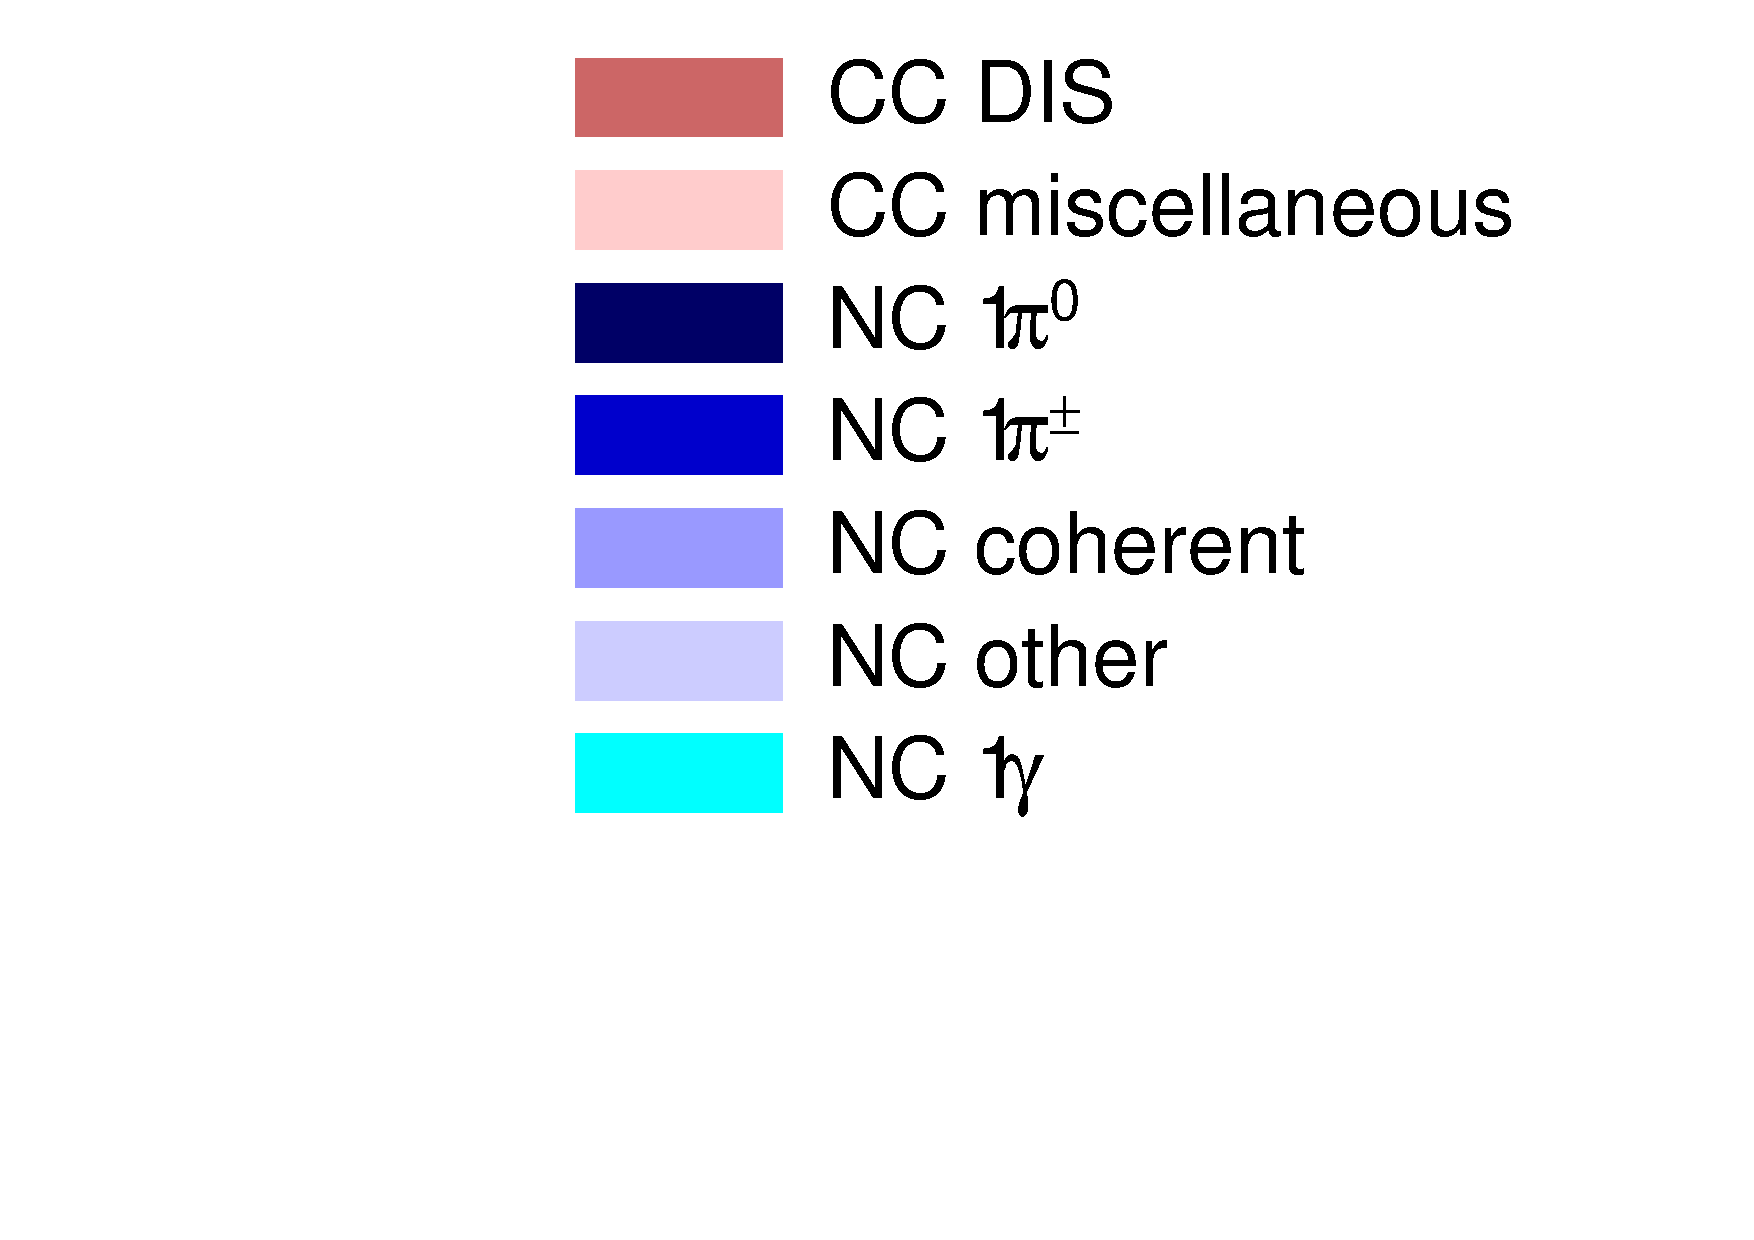
\includegraphics[width=\linewidth, trim={5mm 0mm 30mm 80mm}, clip]{figs/legend2}
\end{subfigure}

\begin{subfigure}{0.49\textwidth}
  \centering
  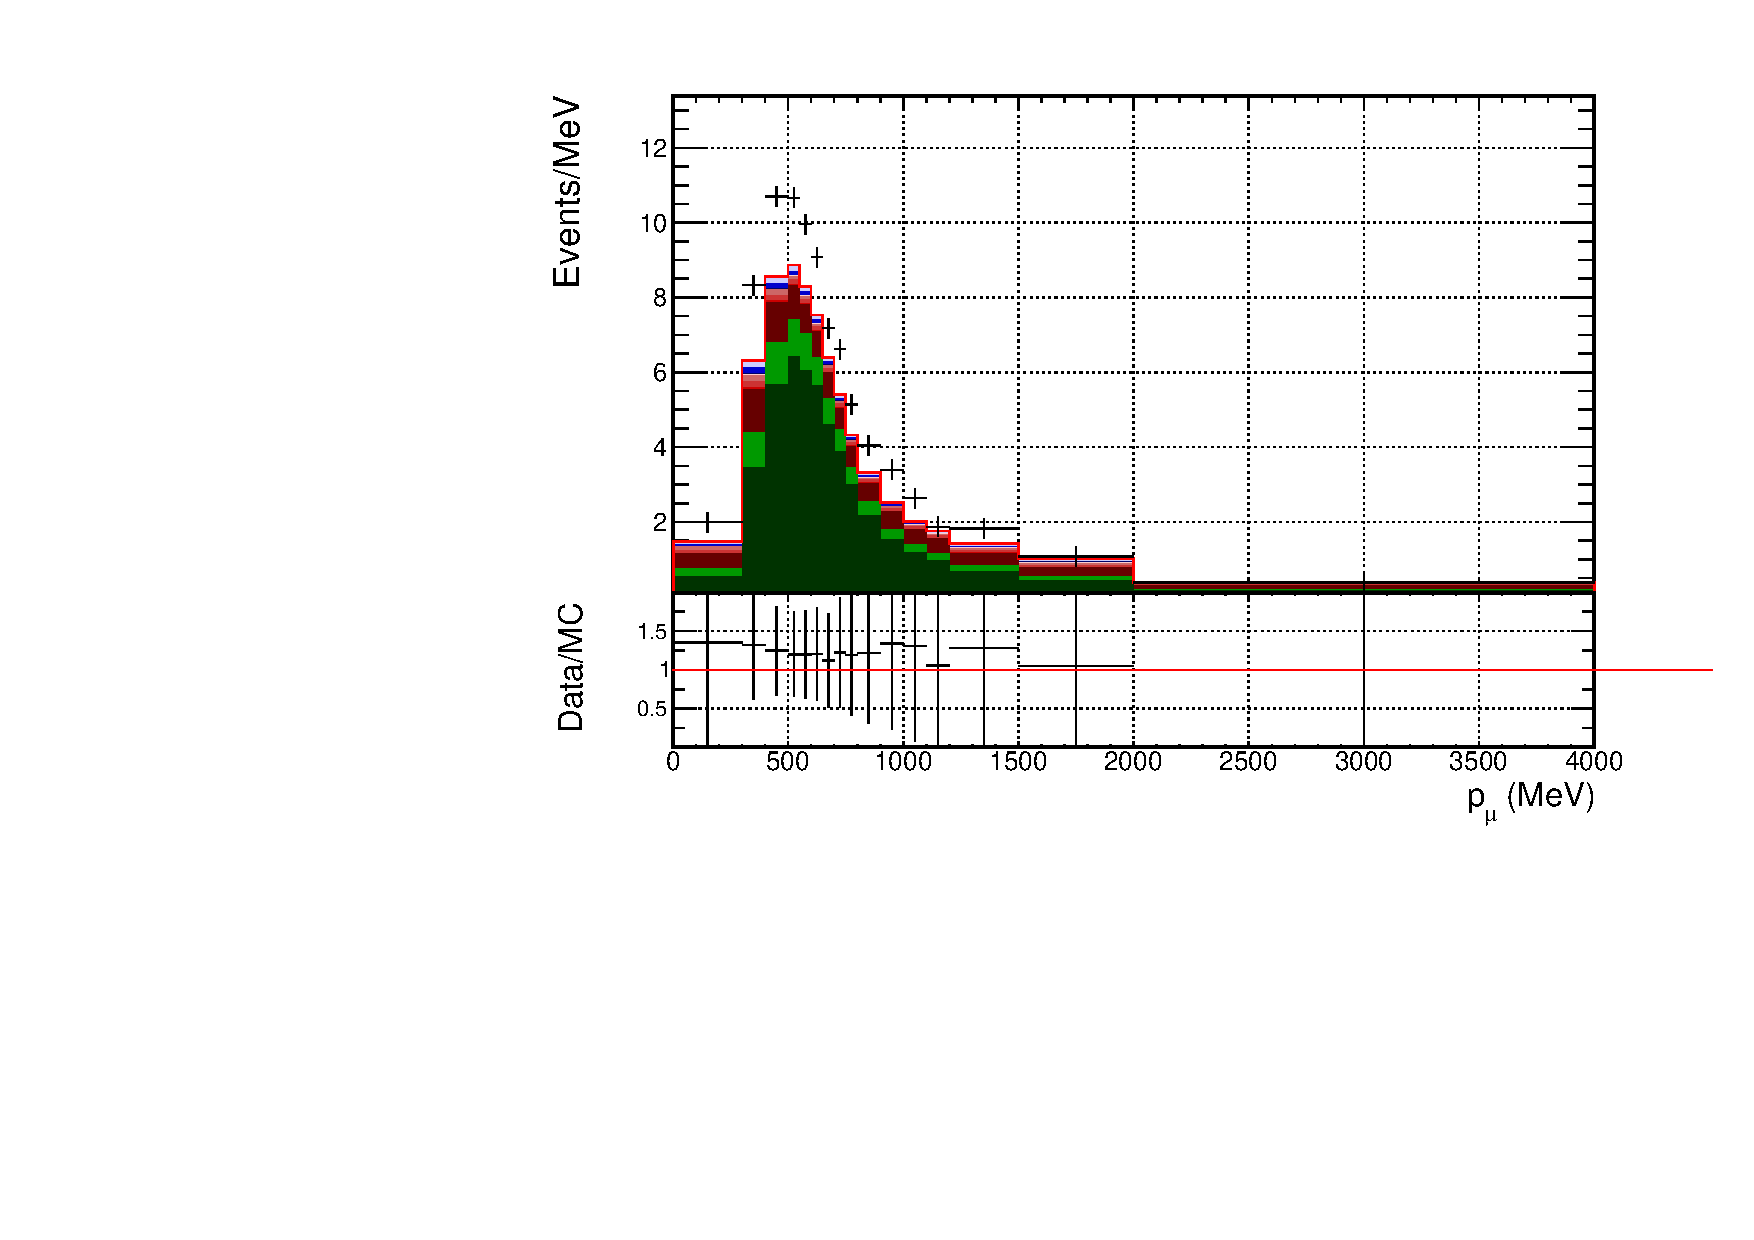
\includegraphics[width=\textwidth]{figs/FGD1_anti-numuCC_0pi_p}
  \caption{FGD1 RHC $\bar{\nu_{\mu}}$ 0$\pi$}
\end{subfigure}
\begin{subfigure}{0.49\textwidth}
  \centering
  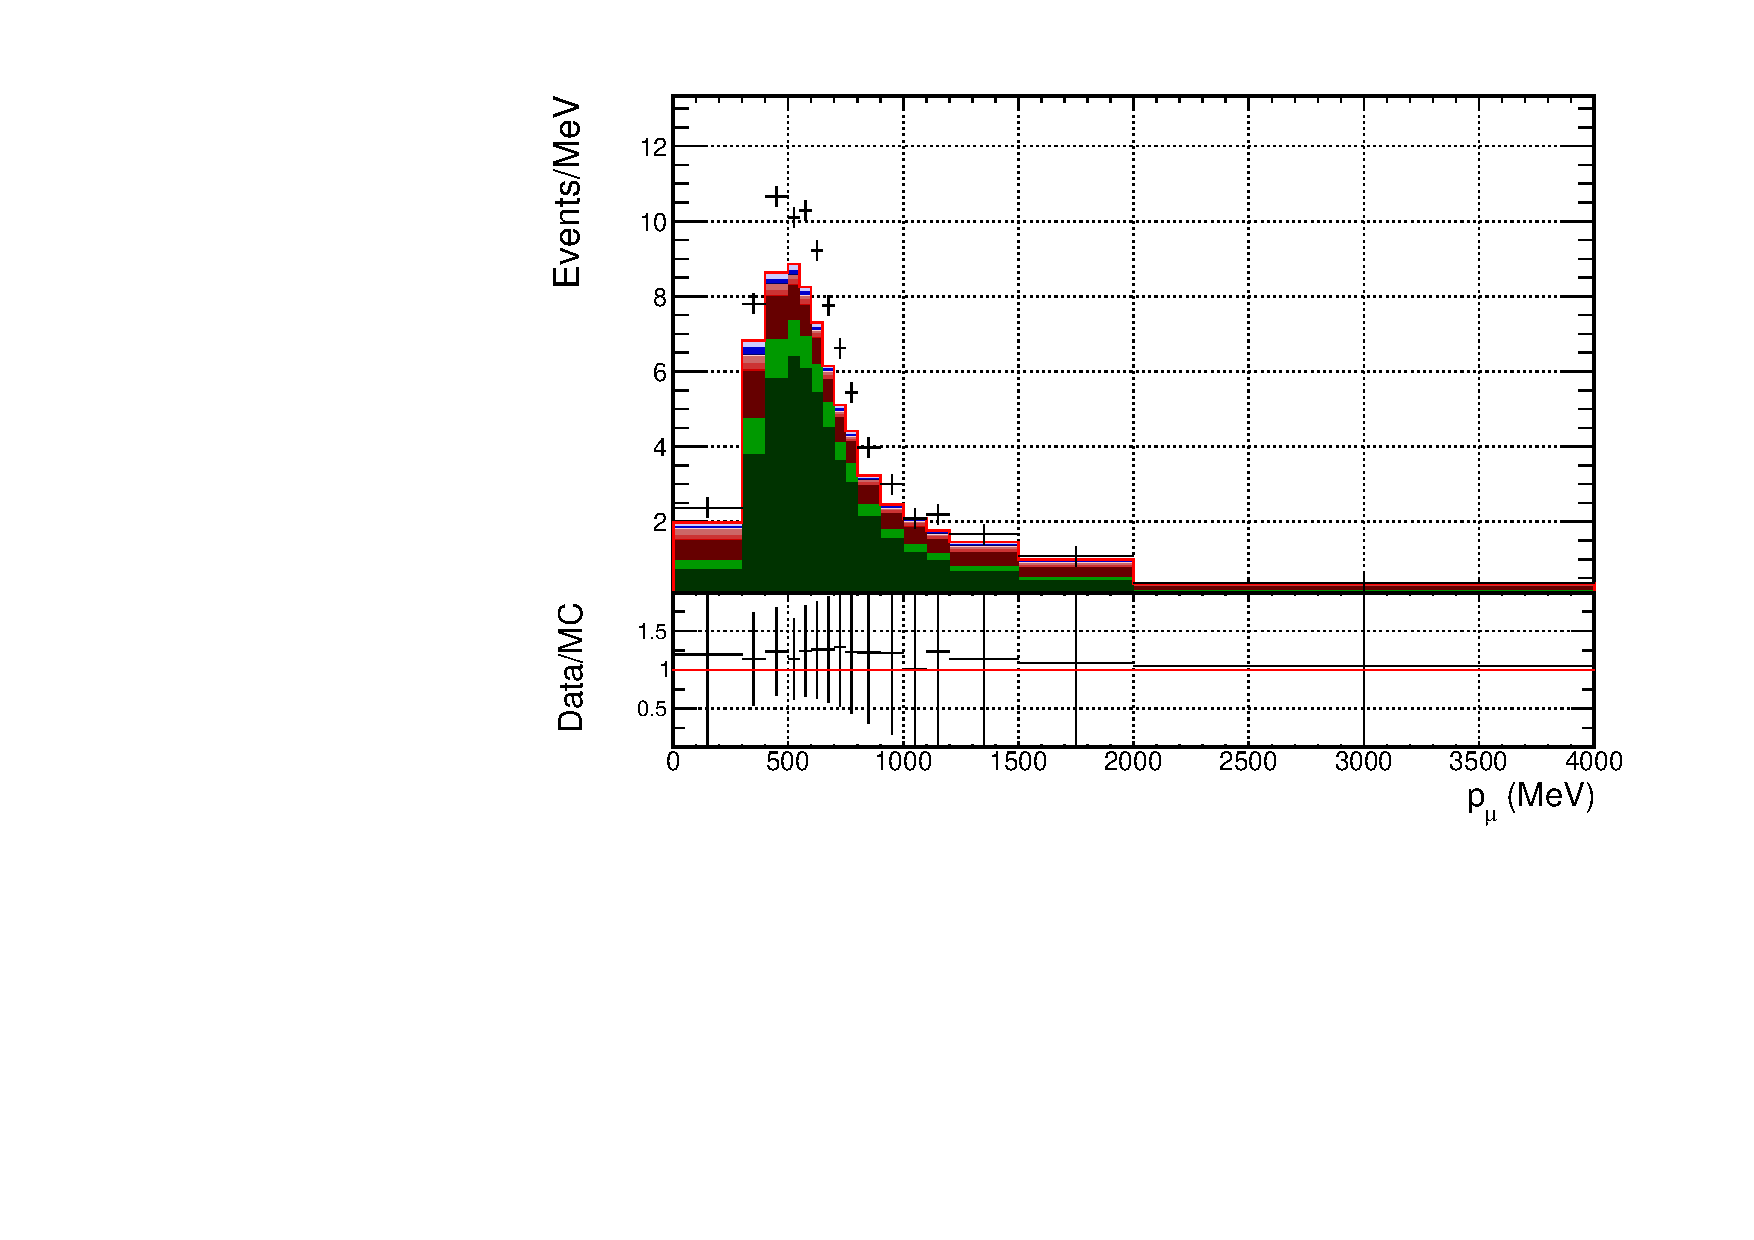
\includegraphics[width=\textwidth]{figs/FGD2_anti-numuCC_0pi_p}
  \caption{FGD2 RHC $\bar{\nu_{\mu}}$ 0$\pi$}
\end{subfigure}

\begin{subfigure}{0.49\textwidth}
  \centering
  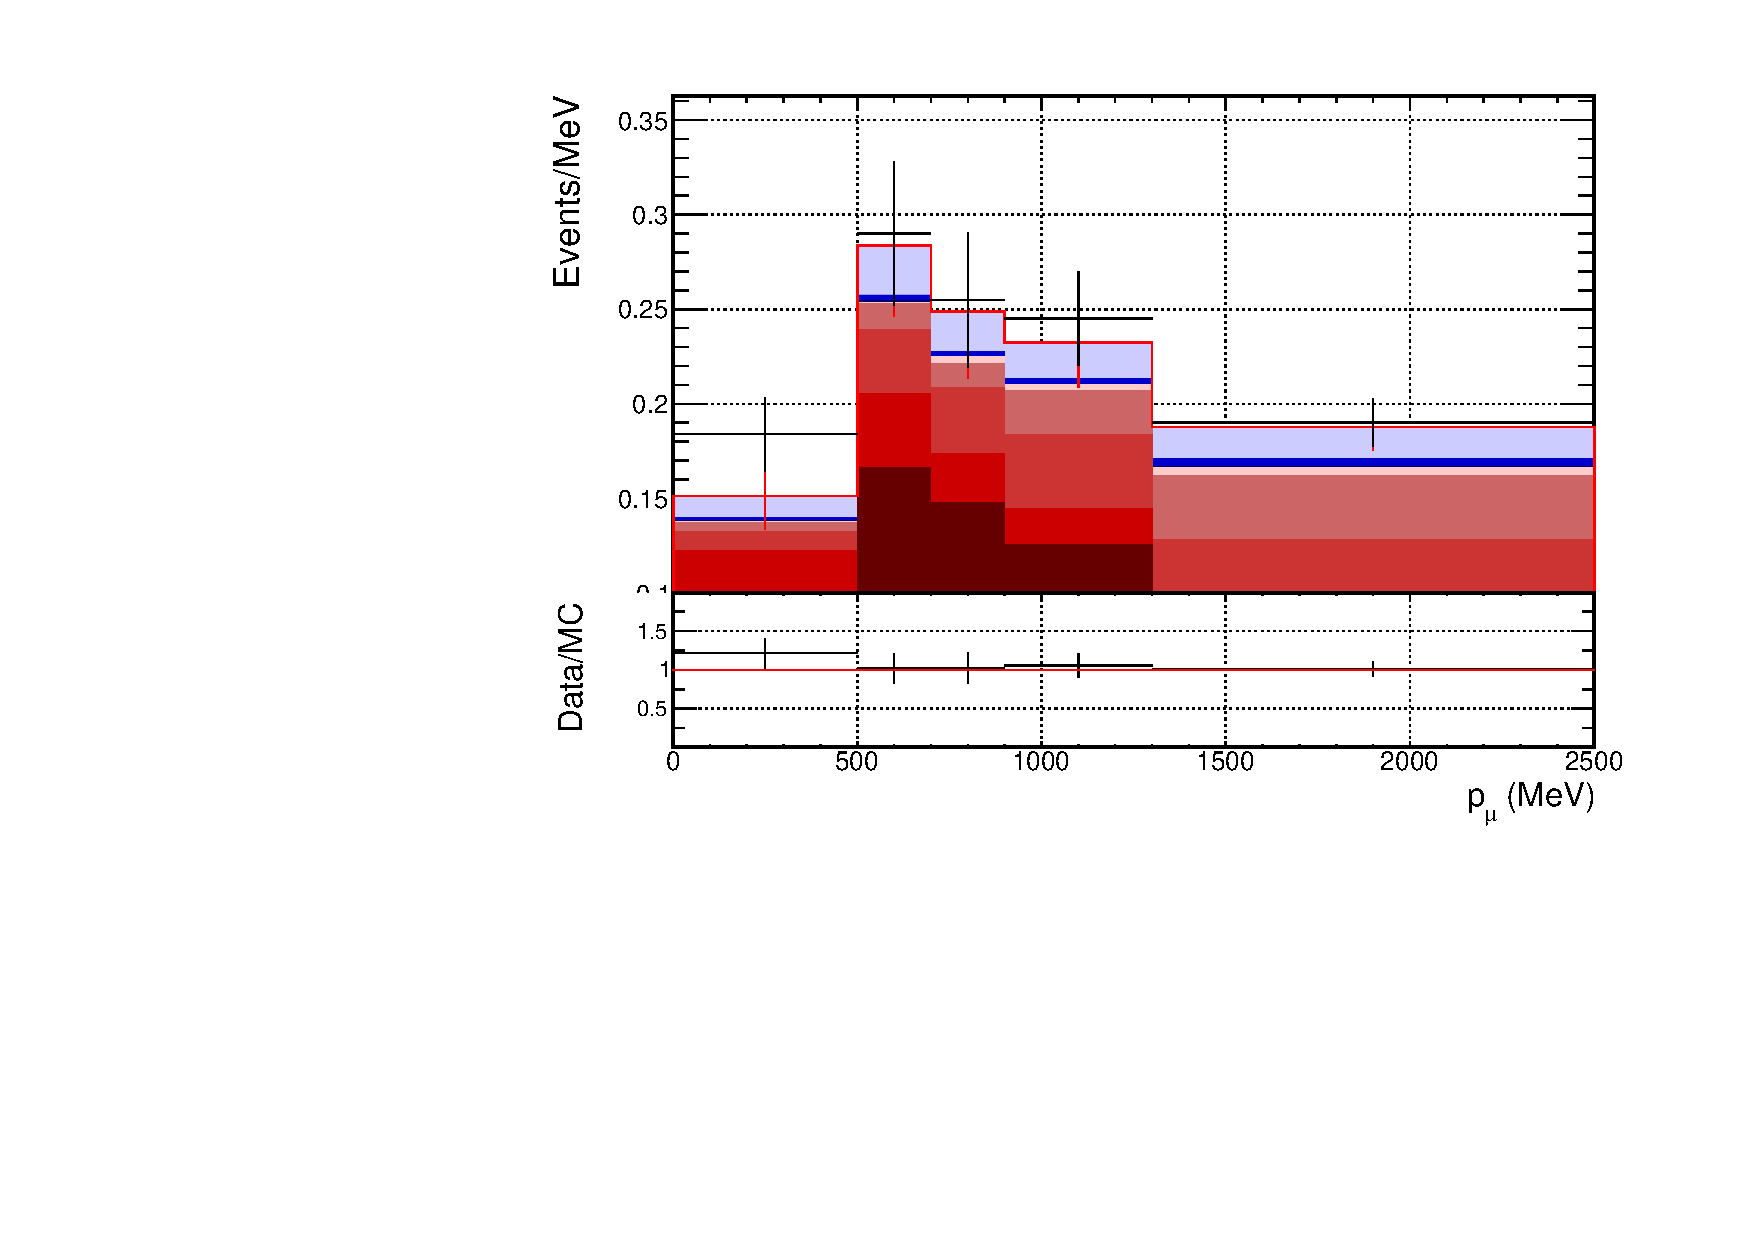
\includegraphics[width=\textwidth]{figs/FGD1_anti-numuCC_1pi_p}
  \caption{FGD1 RHC $\bar{\nu_{\mu}}$ 1$\pi$}
\end{subfigure}
\centering
\begin{subfigure}{0.49\textwidth}
  \centering
  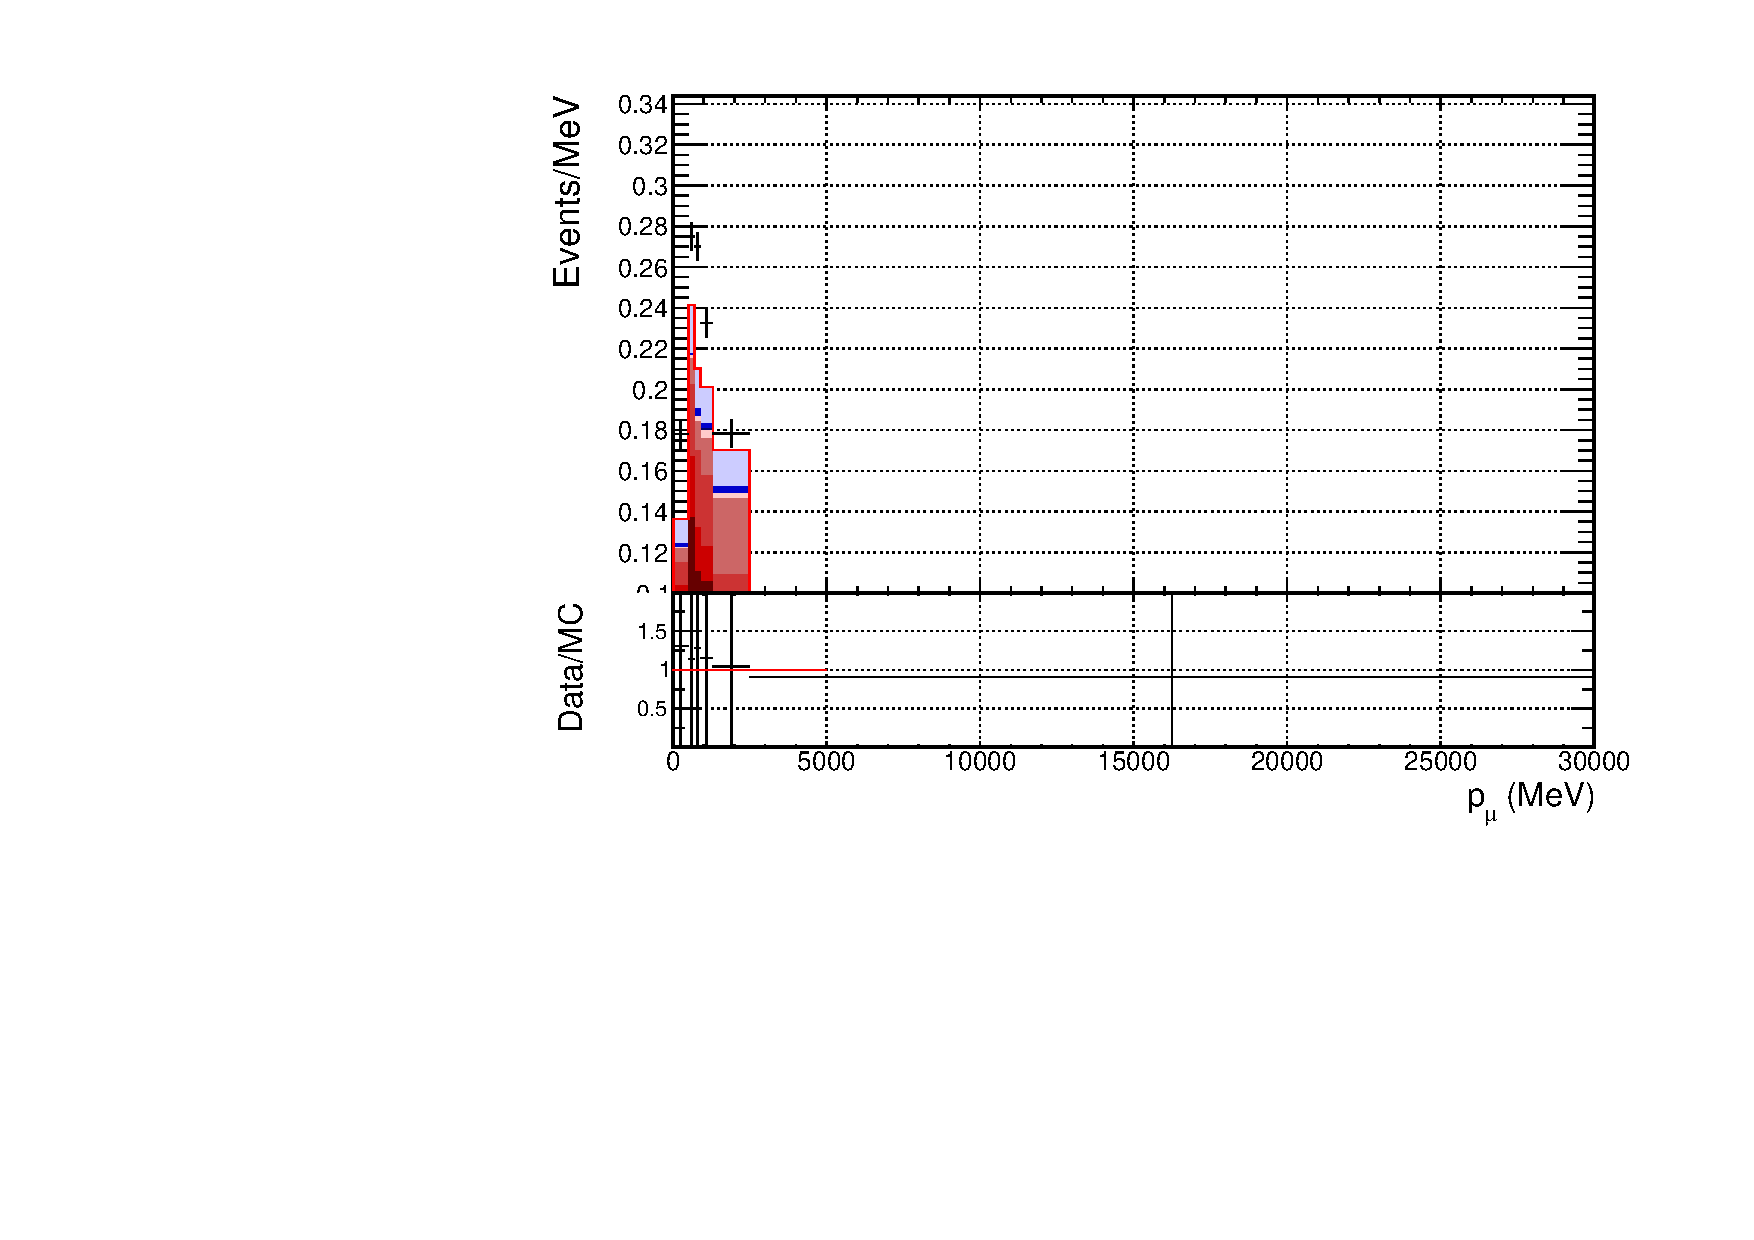
\includegraphics[width=\textwidth]{figs/FGD2_anti-numuCC_1pi_p}
  \caption{FGD2 RHC $\bar{\nu_{\mu}}$ 1$\pi$}
\end{subfigure}

\begin{subfigure}{0.49\textwidth}
  \centering
  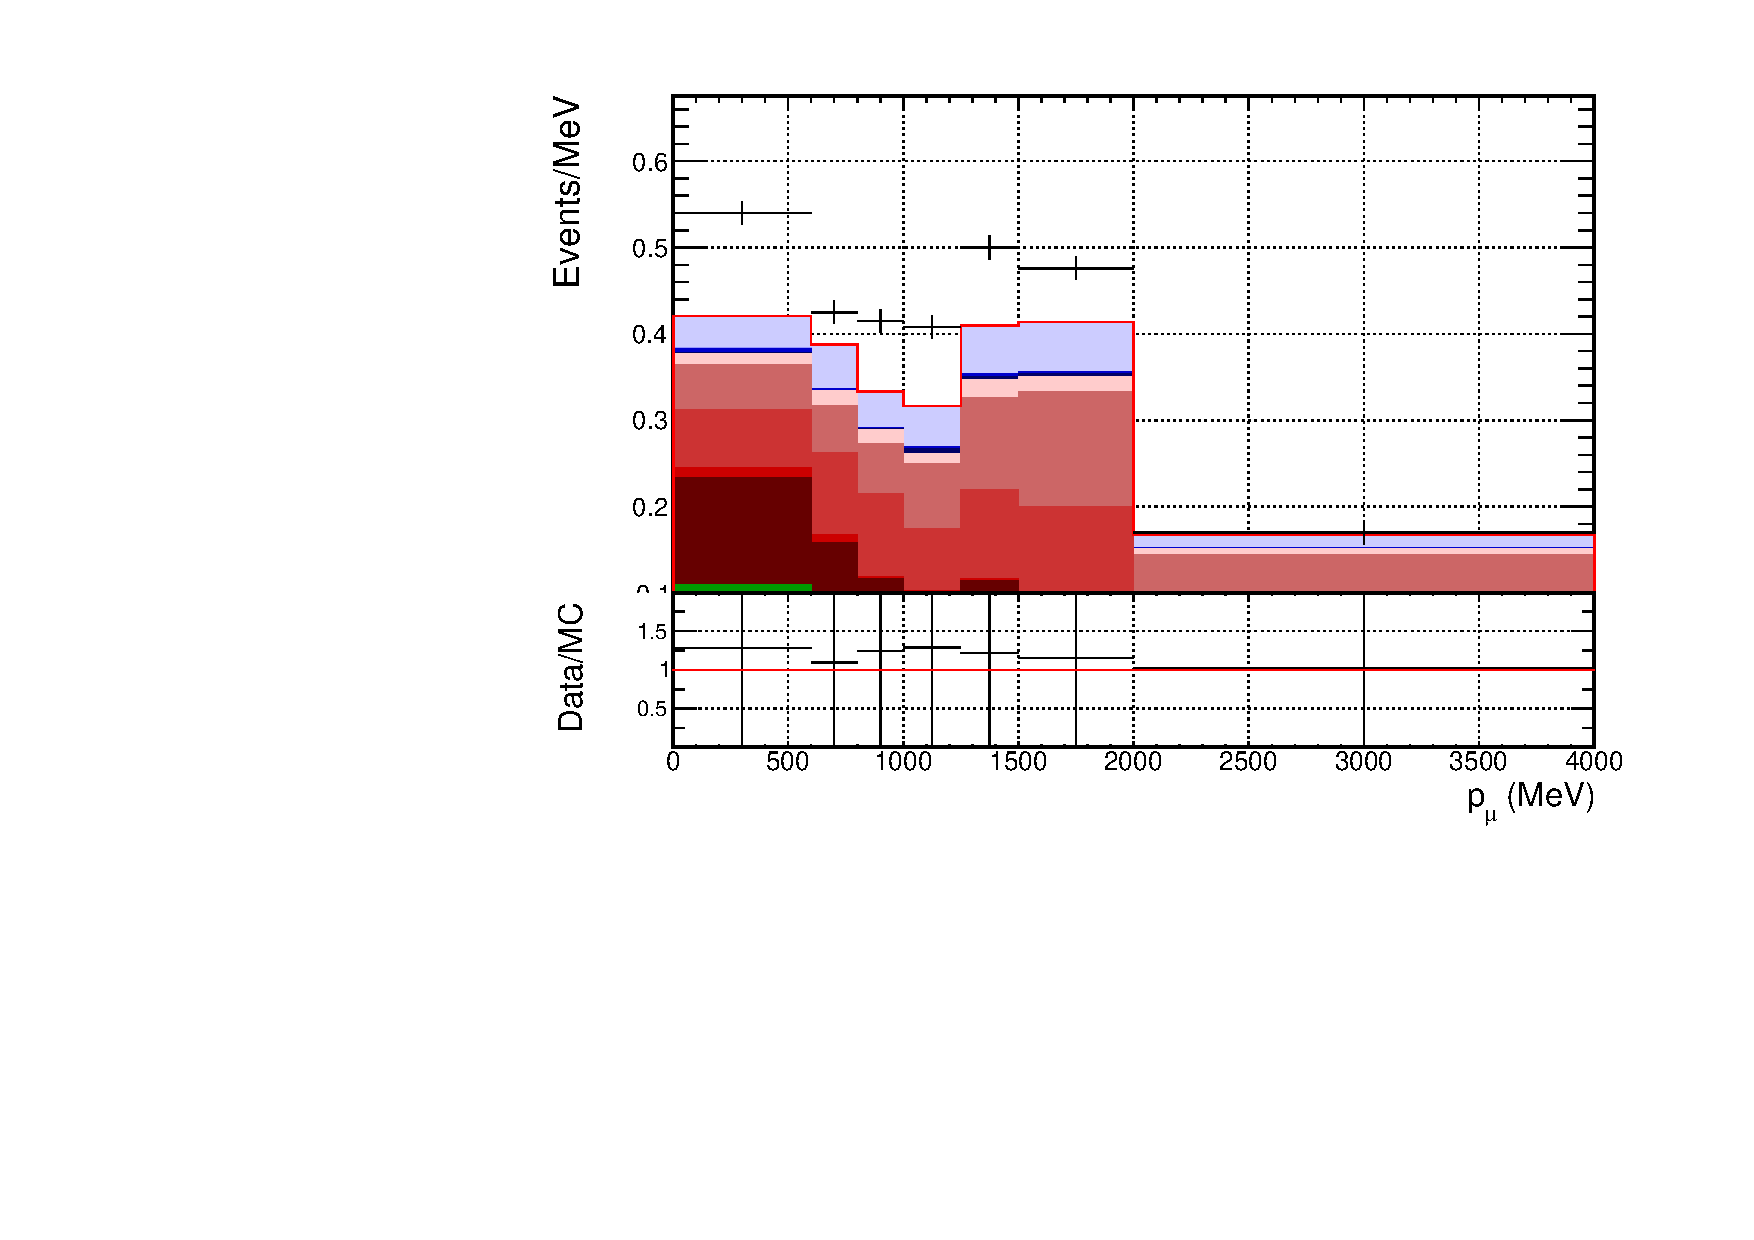
\includegraphics[width=\textwidth]{figs/FGD1_anti-numuCC_other_p}
  \caption{FGD1 RHC $\bar{\nu_{\mu}}$ Other}
\end{subfigure}
\begin{subfigure}{0.49\textwidth}
  \centering
  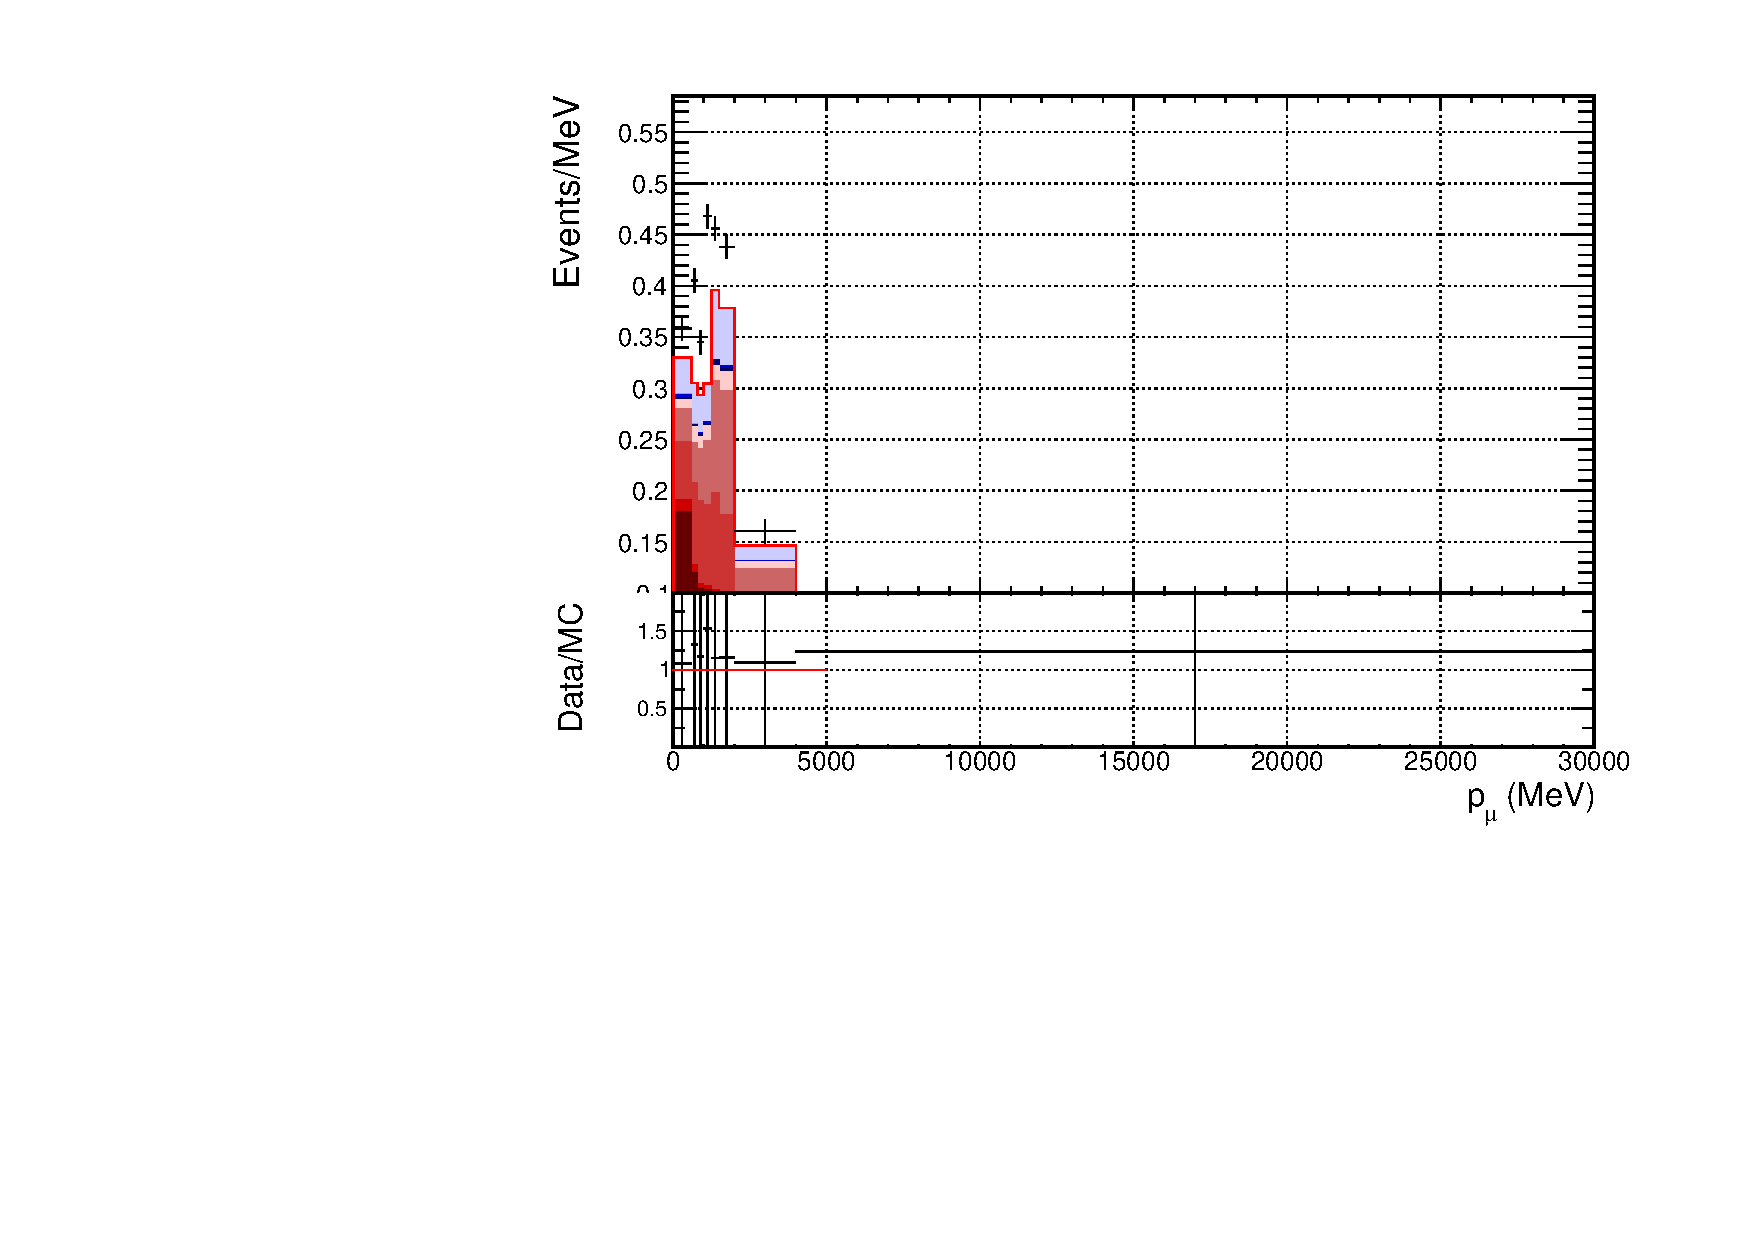
\includegraphics[width=\textwidth]{figs/FGD2_anti-numuCC_other_p}
  \caption{FGD2 RHC $\bar{\nu_{\mu}}$ Other}
\end{subfigure}
\caption{$p_{\mu}$ projections of data and nominal MC broken down by interaction mode for RHC \numub selections.}
\label{fig:pstack_rhc_numub}
\end{figure}

\begin{figure}[!htbp]
\centering
\begin{subfigure}{.24\textwidth}
  \centering
  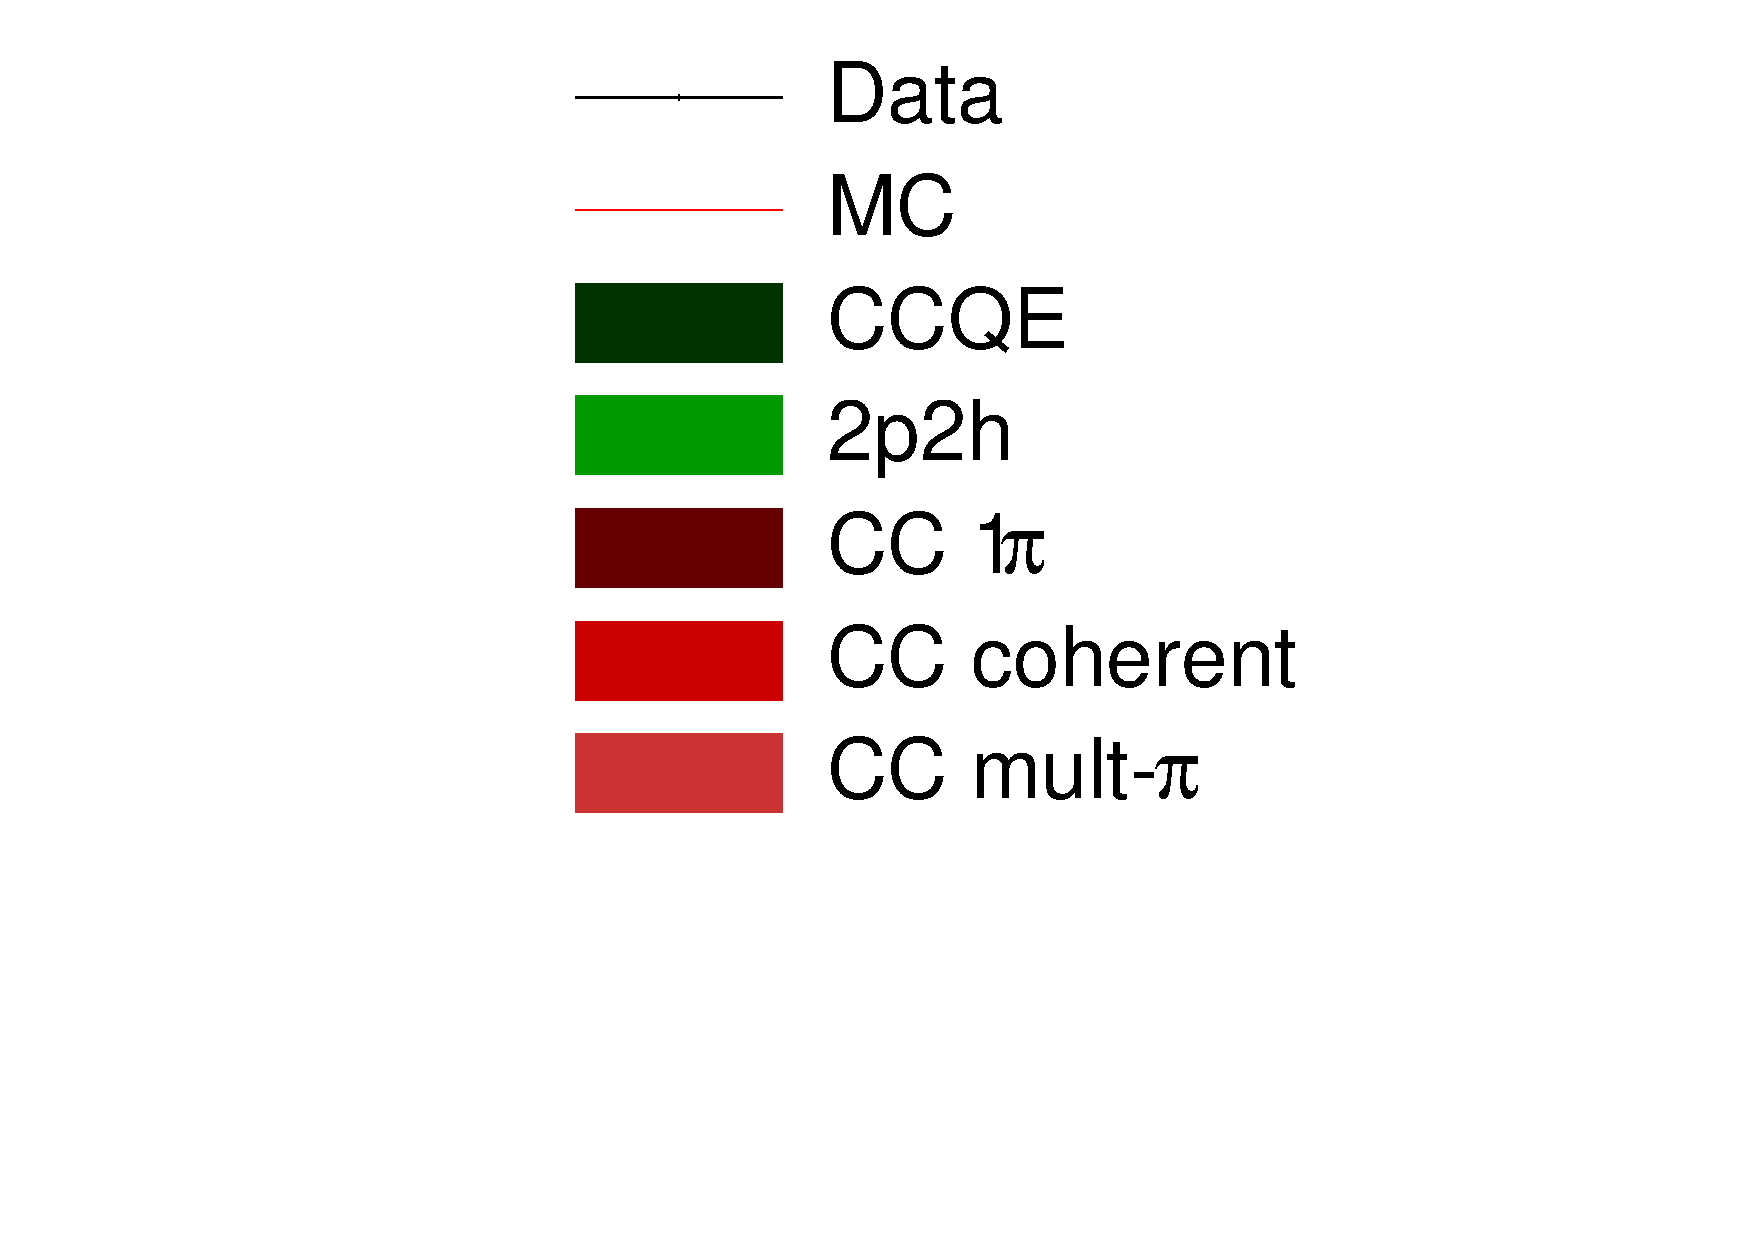
\includegraphics[width=\linewidth, trim={5mm 60mm 30mm 0mm}, clip]{figs/legend}
\end{subfigure}
\begin{subfigure}{.24\textwidth}
  \centering
  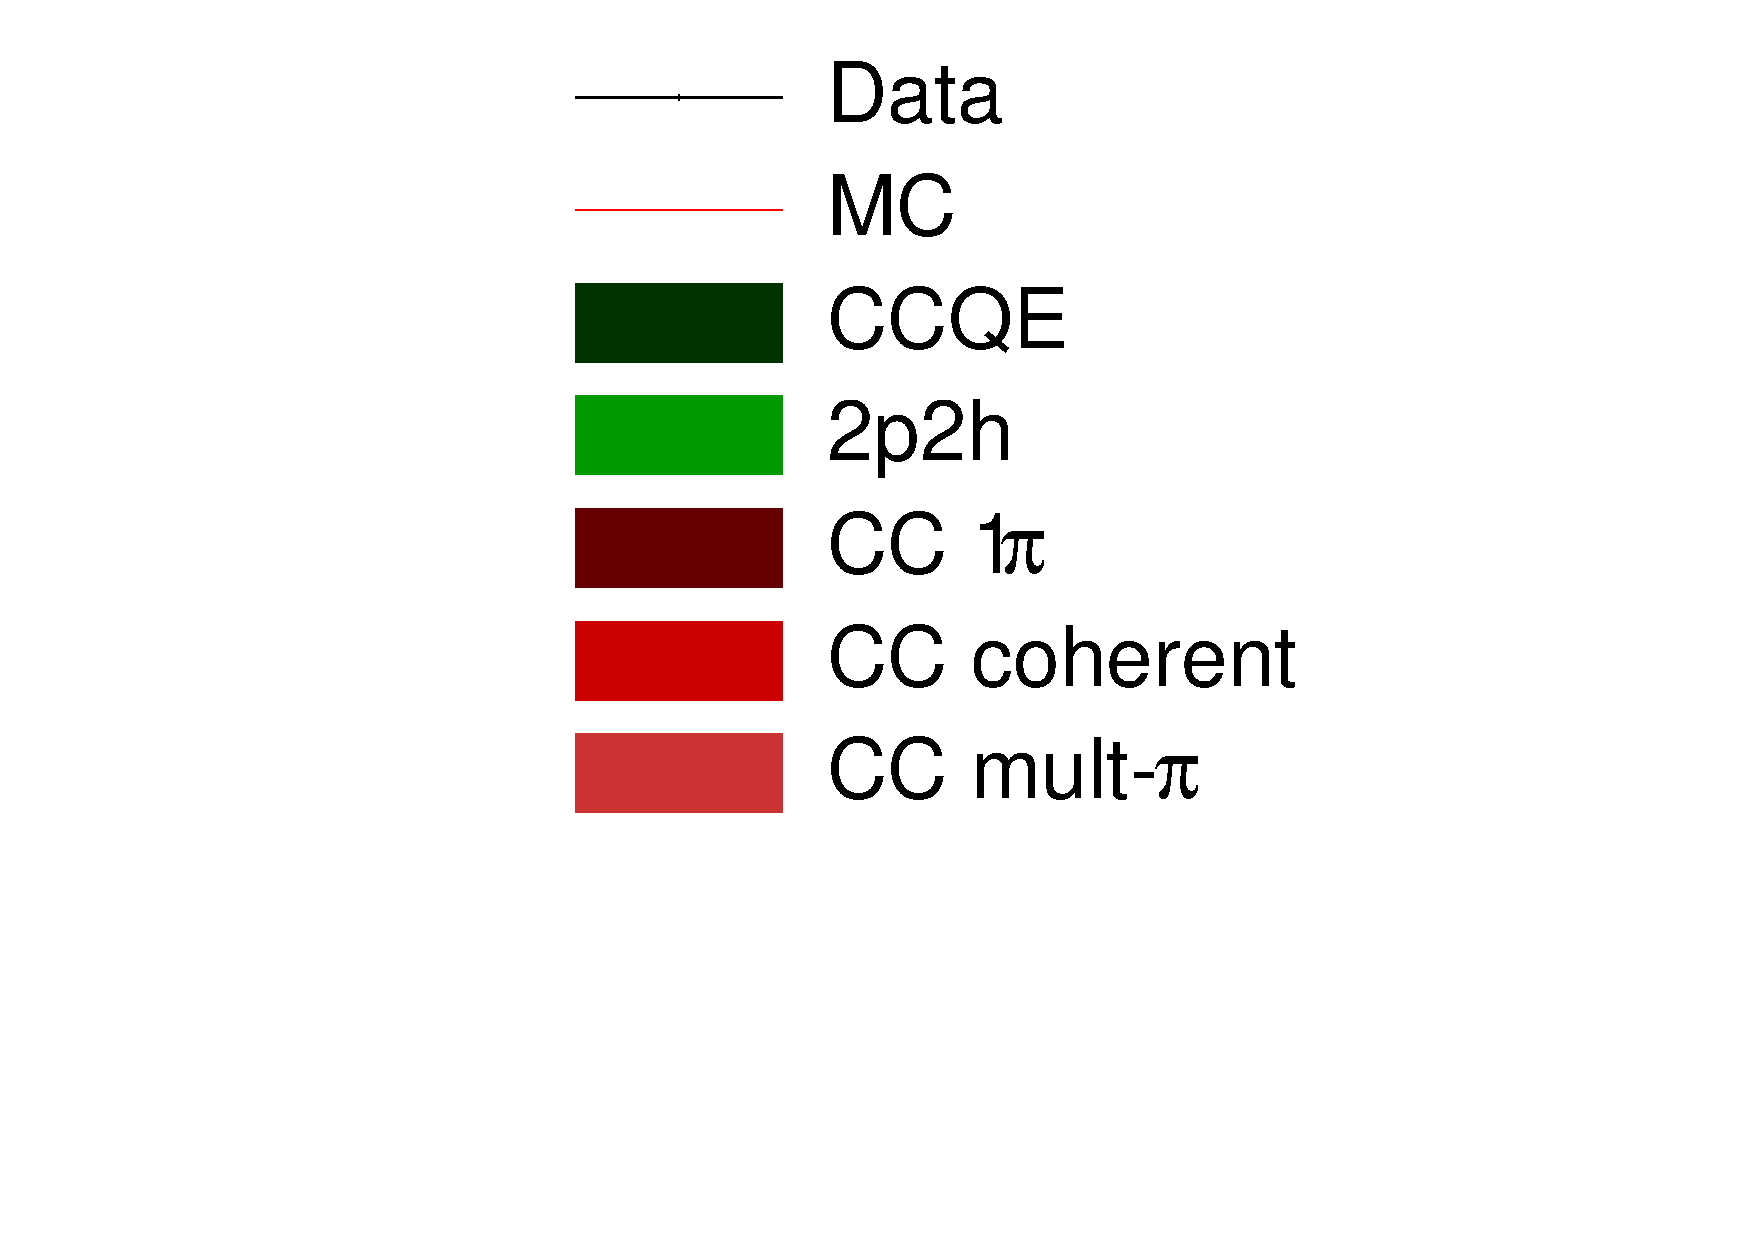
\includegraphics[width=\linewidth, trim={5mm 0mm 30mm 80mm}, clip]{figs/legend}
\end{subfigure}
\begin{subfigure}{.24\textwidth}
  \centering
  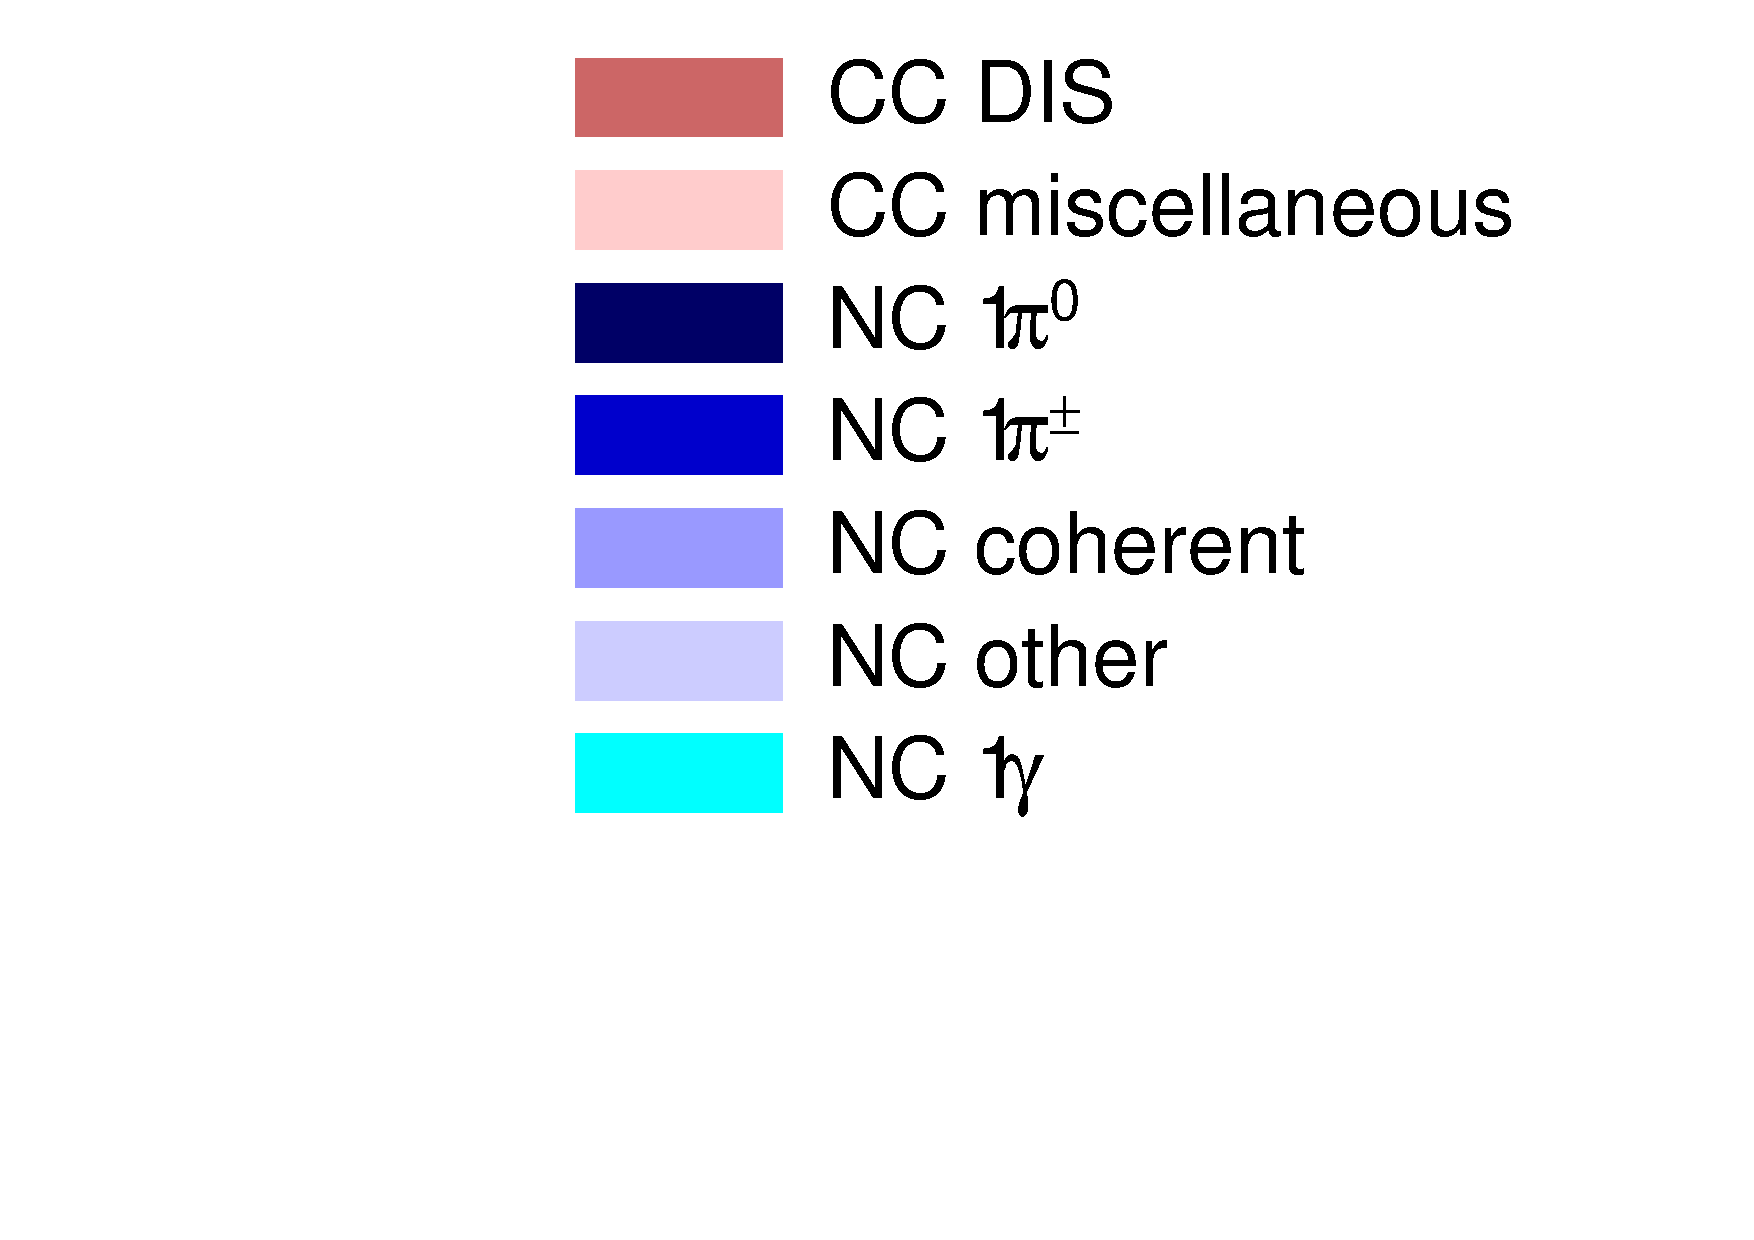
\includegraphics[width=\linewidth, trim={5mm 60mm 30mm 0mm}, clip]{figs/legend2}
\end{subfigure}
\begin{subfigure}{.24\textwidth}
  \centering
  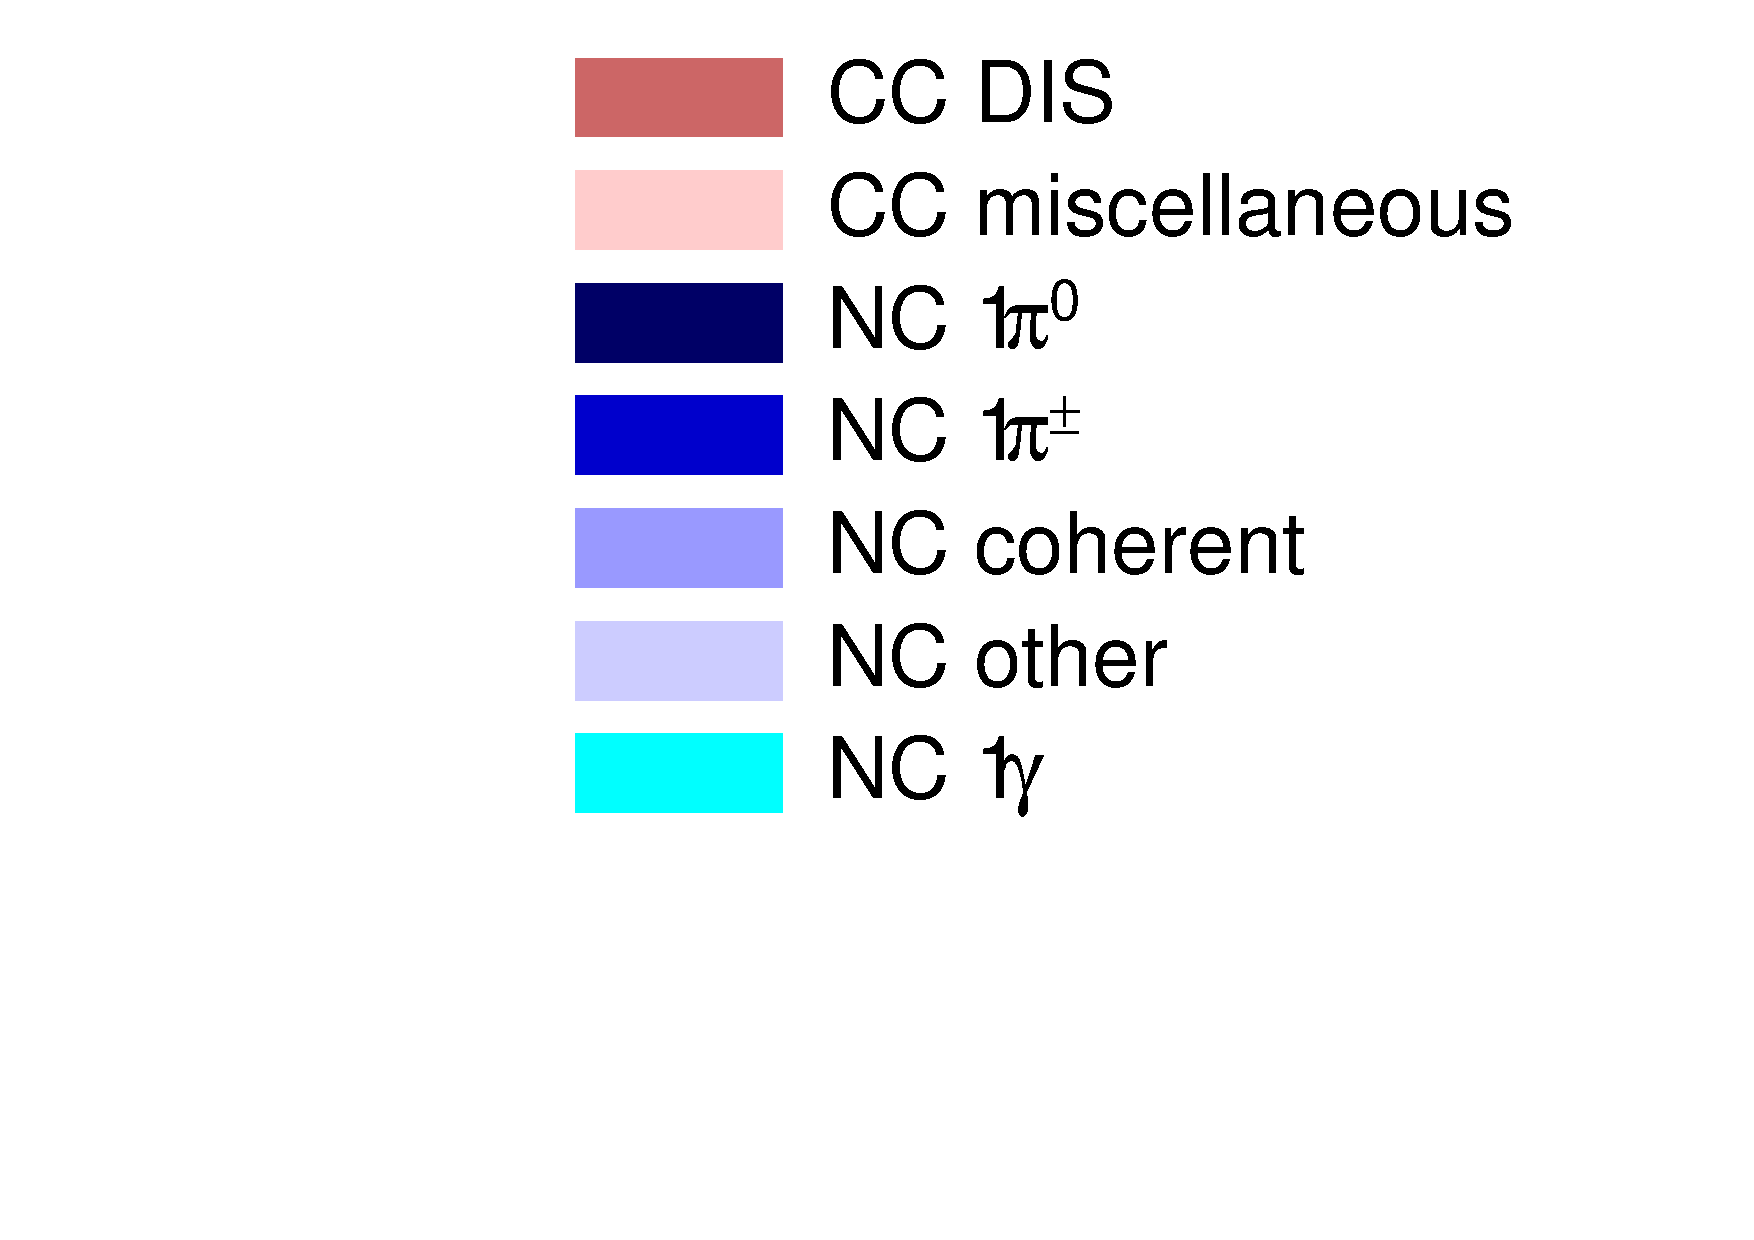
\includegraphics[width=\linewidth, trim={5mm 0mm 30mm 80mm}, clip]{figs/legend2}
\end{subfigure}

\begin{subfigure}{0.49\textwidth}
  \centering
  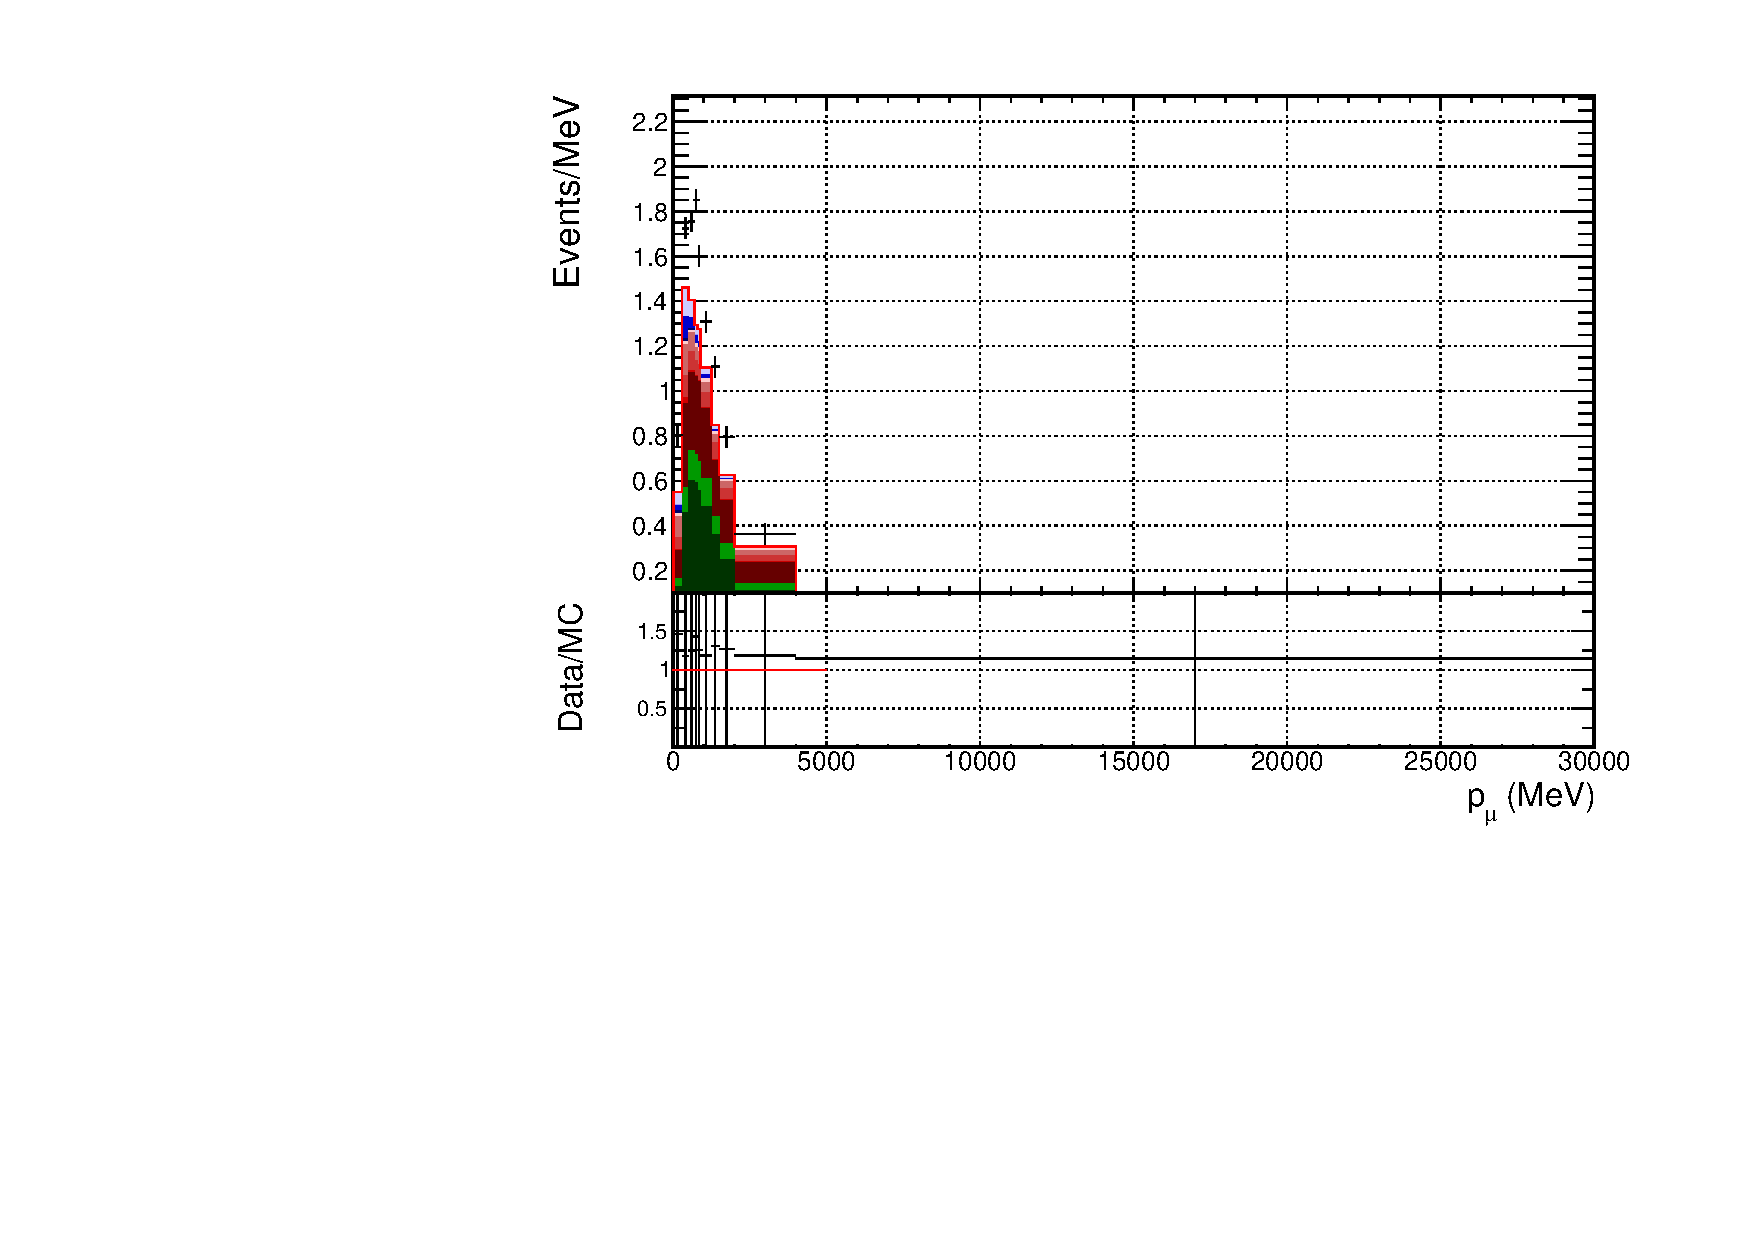
\includegraphics[width=\textwidth]{figs/FGD1_NuMuBkg_CC0pi_in_AntiNu_Mode_p}
  \caption{FGD1 RHC $\nu_{\mu}$ 0$\pi$}
\end{subfigure}
\begin{subfigure}{0.49\textwidth}
  \centering
  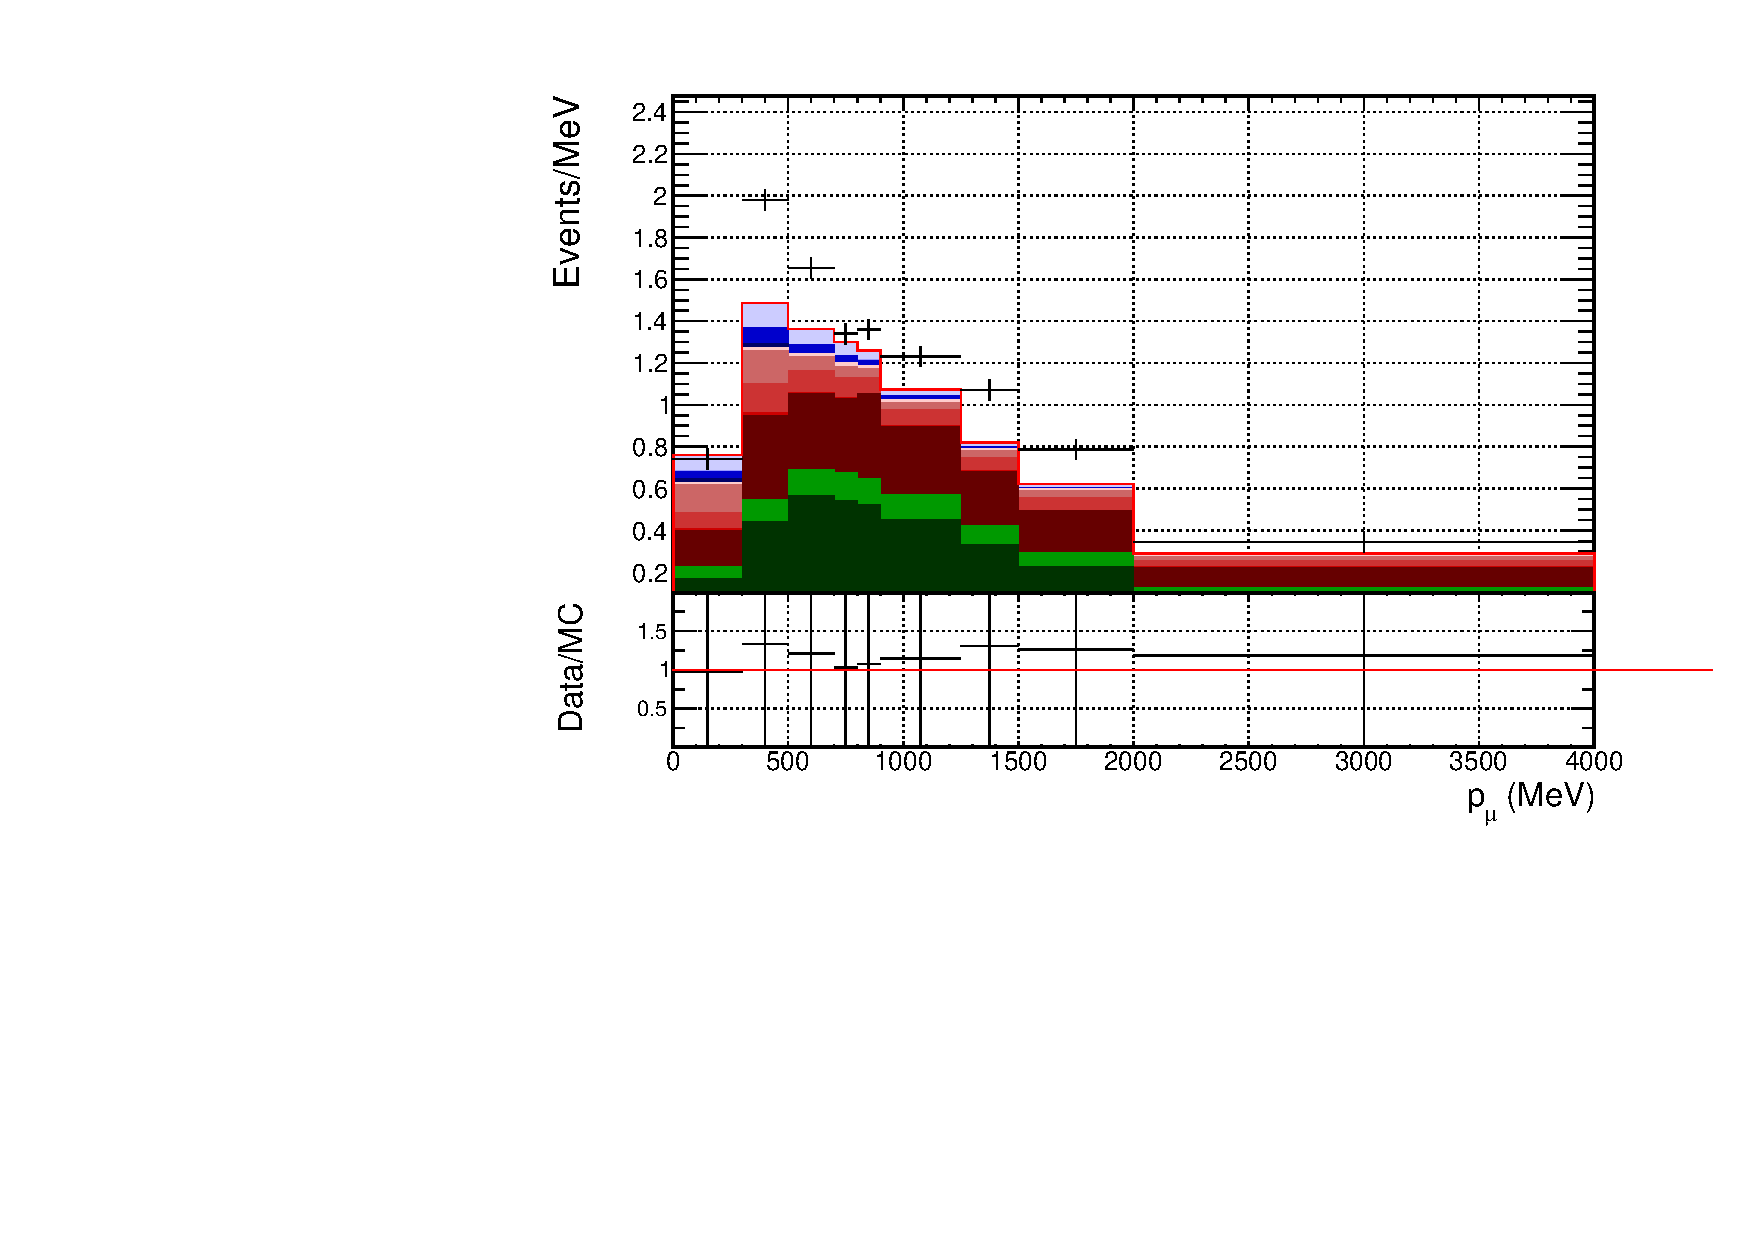
\includegraphics[width=\textwidth]{figs/FGD2_NuMuBkg_CC0pi_in_AntiNu_Mode_p}
  \caption{FGD2 RHC $\nu_{\mu}$ 0$\pi$}
\end{subfigure}

\begin{subfigure}{0.49\textwidth}
  \centering
  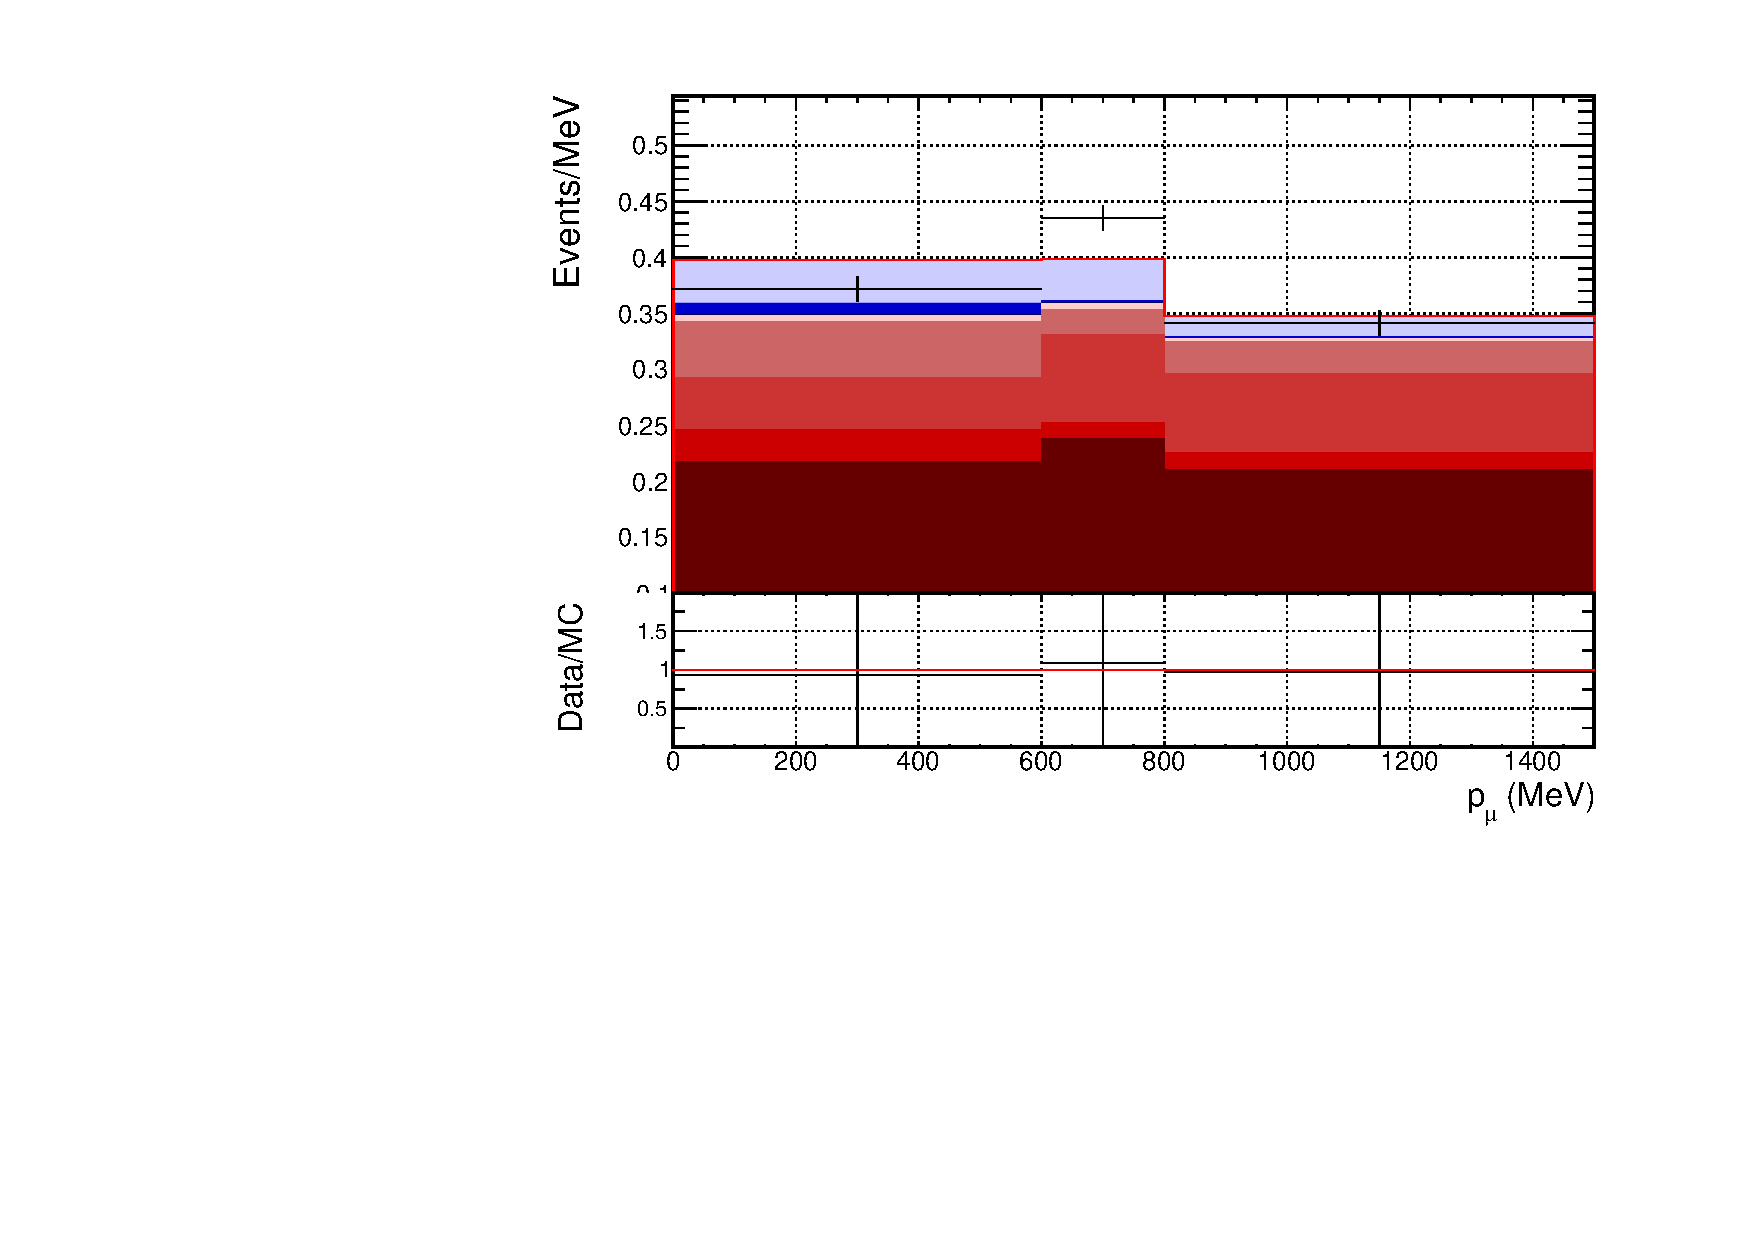
\includegraphics[width=\textwidth]{figs/FGD1_NuMuBkg_CC1pi_in_AntiNu_Mode_p}
  \caption{FGD1 RHC $\nu_{\mu}$ 1$\pi$}
\end{subfigure}
\begin{subfigure}{0.49\textwidth}
  \centering
  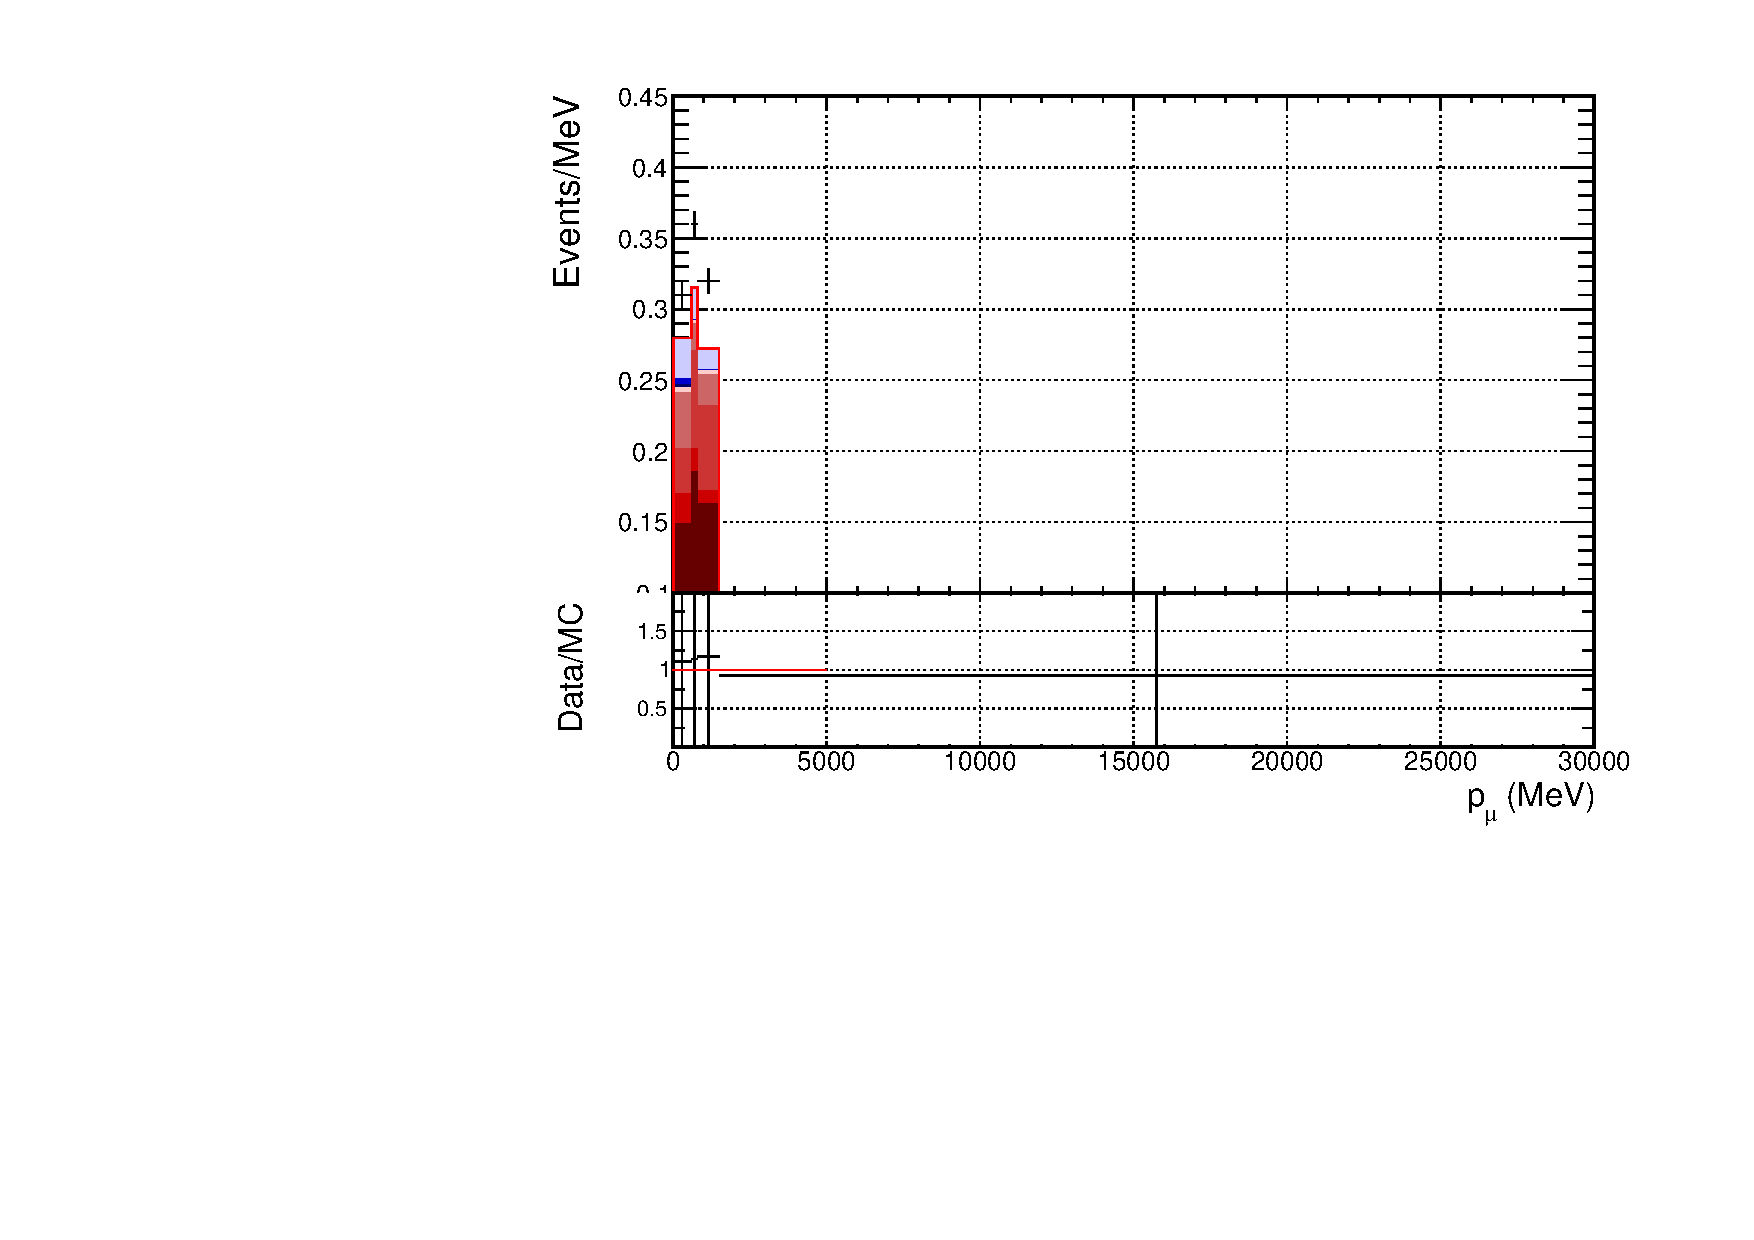
\includegraphics[width=\textwidth]{figs/FGD2_NuMuBkg_CC1pi_in_AntiNu_Mode_p}
  \caption{FGD2 RHC $\nu_{\mu}$ 1$\pi$}
\end{subfigure}

\begin{subfigure}{0.49\textwidth}
  \centering
  \includegraphics[width=\textwidth]{figs/FGD1_NuMuBkg_CCOther_in_AntiNu_Mode_p}
  \caption{FGD1 RHC $\nu_{\mu}$ Other}
\end{subfigure}
\begin{subfigure}{0.49\textwidth}
  \centering
  \includegraphics[width=\textwidth]{figs/FGD2_NuMuBkg_CCOther_in_AntiNu_Mode_p}
  \caption{FGD2 RHC $\nu_{\mu}$ Other}
\end{subfigure}
\caption{$p_{\mu}$ projections of data and nominal MC broken down by interaction mode for RHC \numu selections.}
\label{fig:pstack_rhc_numu}
\end{figure}

The projections onto the cos$\theta_{\mu}$ axis are shown in Appendix \ref{app:nomMC}, along with the data and interaction mode breakdown.

The ratio of data to MC for CC 0$\pi$ and CC Other samples again fluctuates, but always remains $>1$. For the CC 1$\pi$ samples, the ratio is more flat, but at high angle oscillates between the MC over and underestimating the data. The behaviour is consistent across FGD1 and FGD2, showing that the strengths and weaknesses of the modelling are similar for both FGDs.

\FloatBarrier
\section{Log-likelihood Scans}\label{sec:llhscan}

As described in Section \ref{sec:extrac}, the marginalisation effects from extracting correlated and non-Gaussian parameters from the full posterior distribution can cause the fit to appear biased. A full Asimov fit alone, described in Section \ref{sec:asimov}, is therefore not a good method of validating the framework.

Log-likelihood scans are also run as part of the validations. The nominal MC is set as the data, and each systematic parameter is varied one at a time to 150 equally spaced points from -1$\sigma$ to +1$\sigma$. At each step, the MC is reweighted and the total likelihood from all contributions calculated. Only the diagonal terms of the covariance matrices are used for the penalty contribution, as otherwise varying one parameter alone could invoke significant penalties from correlations. The scans are therefore not a fully accurate measure of the sensitivity of the fit to constrain each systematic, but a useful validation of the framework.

After each scan, the parameter is reset, and the next parameter in question varied. The likelihood response is expected to be fairly Gaussian for each parameter, as the prior uncertainty is either Gaussian or flat, and most parameters are expected to have a symmetric effect on the number of events in individual bins. The minimum should be at the prior central value of the parameter, and the log-likelihood here should be 0, as at this point the reweighted MC is identical to the nominal MC. No variation of a single parameter should be able to produce a set of distributions more similar to the nominal MC than itself.

The log-likelihood scans for four selected interaction parameters are shown in Figure \ref{fig:llhxsec}. As expected, the test statistic minimises to 0 at the prior central value of each parameter. The penalty contribution to the log-likelihood dominates for the CC normalisation parameter, due to the prior uncertainty being so small. Conversely, the 2p2h $^{12}$C to $^{16}$O normalisation parameter has a weaker prior and therefore a larger contribution from the sample likelihood. The likelihood for the $0.05 < Q^2 < 0.10$ GeV$^2$ normalisation parameter is entirely dominated by the sample contribution, as the prior is flat. The CC DIS and multi-$\pi$ $\bar{\nu}$ normalisation parameter has more balanced contributions from both the sample and penalty likelihoods.

\begin{figure}[!htbp]
\centering
\begin{subfigure}{.49\textwidth}
  \centering
  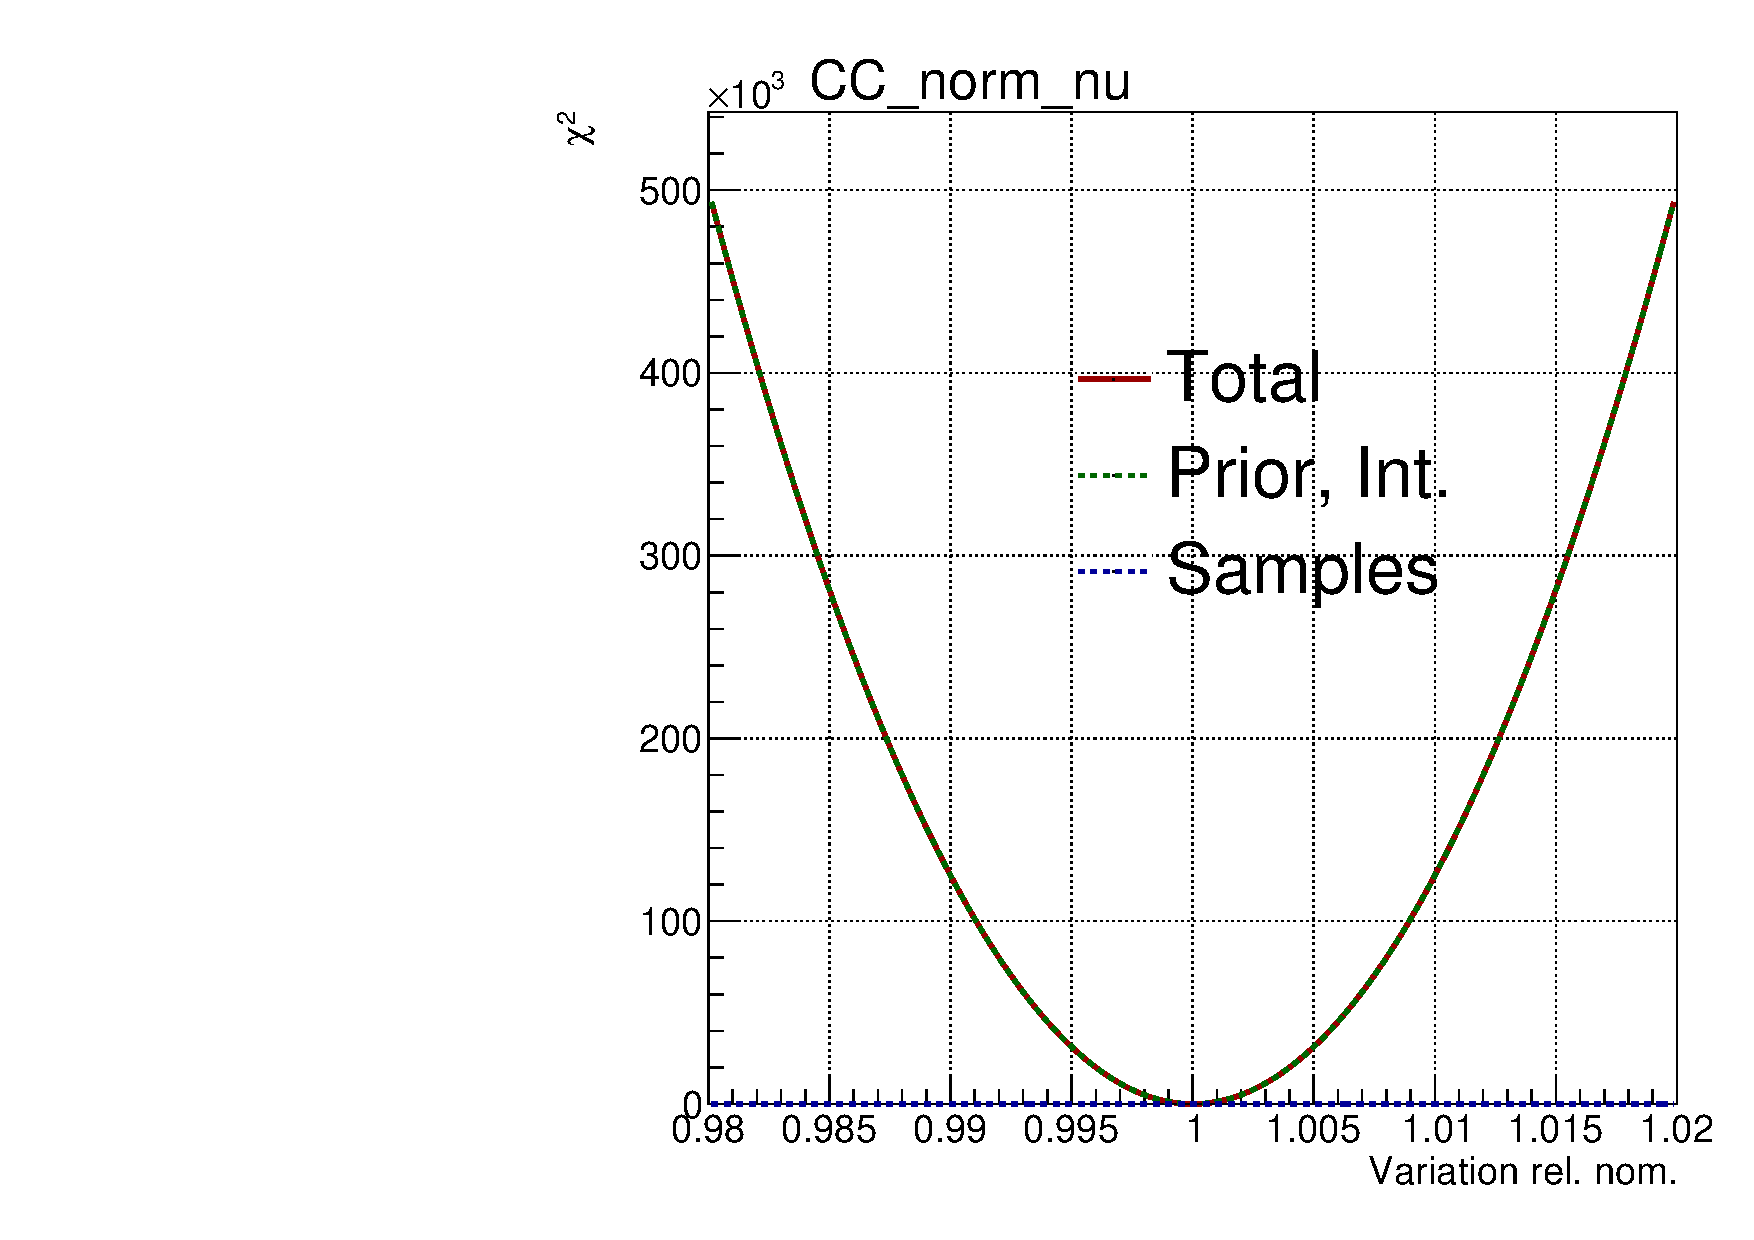
\includegraphics[width=0.7\linewidth]{figs/llh/CC_norm_nu_llh.pdf}
  \caption{CC normalisation $\nu$}
\end{subfigure}
\begin{subfigure}{.49\textwidth}
  \centering
  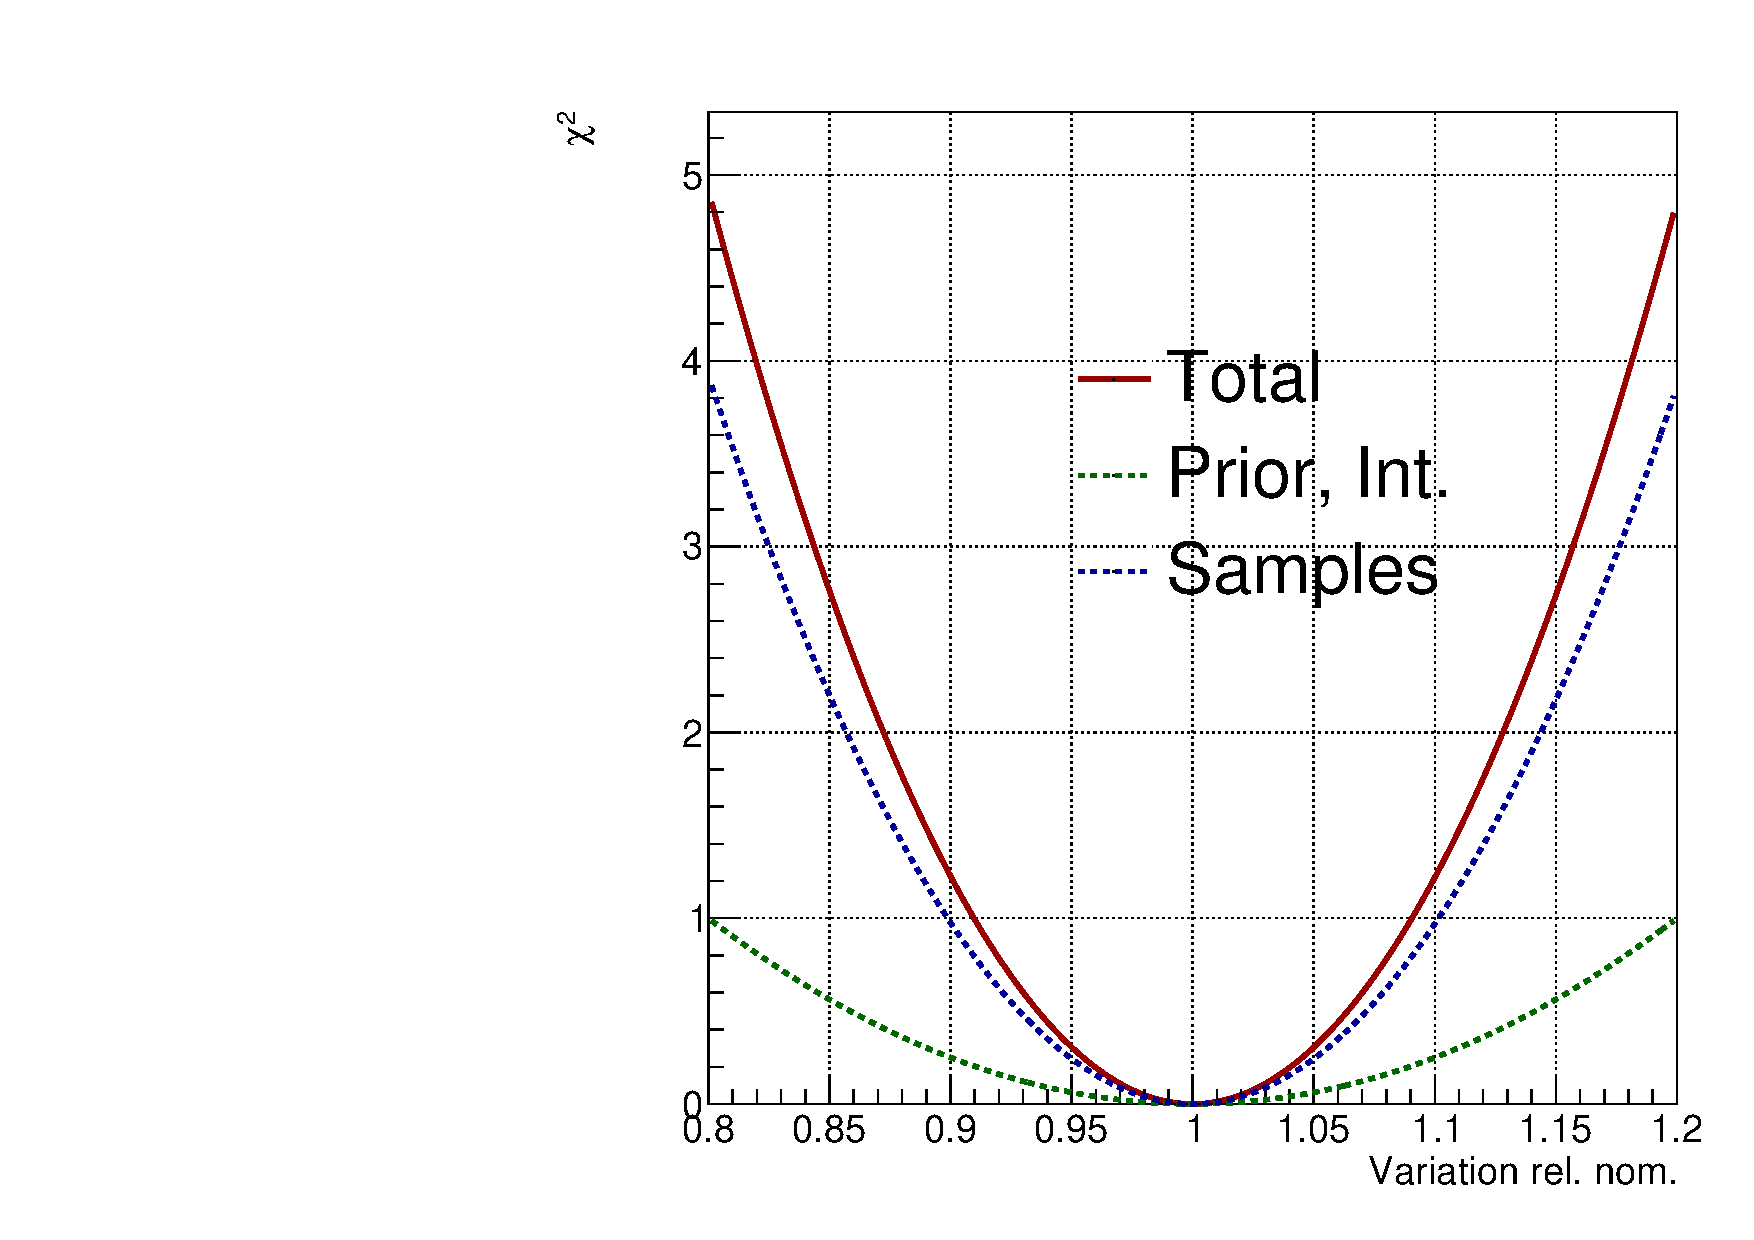
\includegraphics[width=0.7\linewidth]{figs/llh/2p2h_normCtoO_llh.pdf}
  \caption{2p2h $^{12}$C  to $^{16}$O normalisation}
\end{subfigure}
\begin{subfigure}{.49\textwidth}
  \centering
  \includegraphics[width=0.7\linewidth]{figs/llh/Q2_norm_1_llh.pdf}
  \caption{$0.05 < Q^2 < 0.10$ normalisation}
\end{subfigure}
\begin{subfigure}{.49\textwidth}
  \centering
  \includegraphics[width=0.7\linewidth]{figs/llh/CC_DIS_MultPi_Norm_Nubar_llh.pdf}
  \caption{CC DIS and multi-$\pi$ normalisation}
\end{subfigure}
\caption{Log-likelihood scans for selected interaction parameters. CC norm. $\nu$ has a tight prior uncertainty that dominates the likelihood, whereas the low $Q^2$ normalisations have a flat prior so the sample is the only contribution. The 2p2h $^{12}$C to $^{16}$O and CC DIS and multi-$\pi$ normalisations have significant contributions from both the sample and prior uncertainty.}
\label{fig:llhxsec} 
\end{figure}

The log-likelihood scans for four selected flux parameters are shown in Figure \ref{fig:llhflux}. The test statistic again minimises to 0 at the prior central value of each parameter, as expected. These parameters all have tight prior uncertainties, and so the penalty terms dominate the likelihoods. For the \SK flux parameters, there is no sample contribution to the likelihood. This is expected as the \SK flux parameters should have no effect on the ND280 samples (apart from through the correlations with ND280 flux parameters, which are not included in these scans). 

\begin{figure}[!htbp]
\centering
\begin{subfigure}{.49\textwidth}
  \centering
  \includegraphics[width=0.7\linewidth]{figs/llh/b_5_llh.pdf}
  \caption{ND280 FHC $\nu_{\mu}$ 1--1.5 GeV}
\end{subfigure}
\begin{subfigure}{.49\textwidth}
  \centering
  \includegraphics[width=0.7\linewidth]{figs/llh/b_12_llh.pdf}
  \caption{ND280 FHC $\nu_{e}$ 0.5--0.7 GeV}
\end{subfigure}
\begin{subfigure}{.49\textwidth}
  \centering
  \includegraphics[width=0.7\linewidth]{figs/llh/b_36_llh.pdf}
  \caption{ND280 RHC $\nu_e$ 2.5--30 GeV}
\end{subfigure}
\begin{subfigure}{.49\textwidth}
  \centering
  \includegraphics[width=0.7\linewidth]{figs/llh/b_52_llh.pdf}
  \caption{\SK RHC $\bar{\nu_{\mu}}$ 0.5--0.6 GeV}
\end{subfigure}
\caption{Log-likelihood scans for selected flux parameters. }
\label{fig:llhflux}
\end{figure}

The log-likelihood scans for four selected ND280 detector parameters are shown in Figure \ref{fig:llhdet}. As expected, the test statistics all minimise to 0 at the prior central value of each parameter. The prior dominates for all regions of $p_{\mu}$--cos$\theta_{\mu}$ in each sample. For the higher statistic regions (eg. FGD1 FHC $\nu_{\mu}$ CC 0$\pi$: 300--1000 MeV, 0.92--0.98), the overall constraint is larger than for the lower statistic regions, (eg. FGD1 FHC $\nu_{\mu}$ CC 1$\pi$: 5000--30000 MeV, -1.0--0.6). 

\begin{figure}[!htbp]
\centering
\begin{subfigure}{.49\textwidth}
  \centering
  \includegraphics[width=0.7\linewidth]{figs/llh/ndd_13_llh.pdf}
  \caption{FGD1 FHC $\nu_{\mu}$ CC 0$\pi$: 300--1000 MeV, 0.92--0.98}
\end{subfigure}
\begin{subfigure}{.49\textwidth}
  \centering
  \includegraphics[width=0.7\linewidth]{figs/llh/ndd_136_llh.pdf}
  \caption{FGD1 FHC $\nu_{\mu}$ CC 1$\pi$: 5000--30000 MeV, -1.0--0.6}
\end{subfigure}
\begin{subfigure}{.49\textwidth}
  \centering
  \includegraphics[width=0.7\linewidth]{figs/llh/ndd_541_llh.pdf}
  \caption{FGD2 RHC $\bar{\nu_{\mu}}$ CC Other: 800--30000 MeV, 0.97--1.0}
\end{subfigure}
\begin{subfigure}{.49\textwidth}
  \centering
  \includegraphics[width=0.7\linewidth]{figs/llh/ndd_556_llh.pdf}
  \caption{FGD1 RHC $\nu_{\mu}$ CC Other: 600--30000 MeV, -1.0--0.7}
\end{subfigure}
\caption{Log-likelihood scans for selected ND280 detector parameters.}
\label{fig:llhdet}
\end{figure}

The sample, prior, and total log-likelihood distributions were compared with the other near detector fitting group, and good agreement was found for all parameters.

\section{Parameter Variations}\label{sec:sigvar}

As a further validation of the fitting framework and models, the parameters are again each set to $\pm1\sigma$, one by one, while all others are held at nominal. Instead of the change in likelihood, here the effect on the event distributions in $p_{\mu}$--cos$\theta_{\mu}$ is inspected. 

One varied interaction parameter for each sample is shown in Figure \ref{fig:sigvars}. The combinations of parameter and sample were selected such that the parameter controls interactions targeted by the sample. The parameter is therefore expected to have a significant and well-understood impact on the shown sample. The selection of parameter and sample was also made such that no parameters are shown more than once. The parameter in question is set to $+1\sigma$ above its nominal value, and the ratio of the reweighted MC to the nominal MC is taken.

\begin{figure}[!htbp]
\centering
\begin{subfigure}{.32\textwidth}
  \centering
  \includegraphics[width=0.85\linewidth]{figs/sig/FGD1_numuCC_0pi_2p2h_norm_nu_+1sig.pdf}
  \caption{FGD1 FHC $\nu_{\mu}$ 0$\pi$: 2p2h Norm. $\nu$ += $1\sigma$}
  \label{fig:sigvar_FGD1_numuCC_0pi}
\end{subfigure}
\begin{subfigure}{.32\textwidth}
  \centering
  \includegraphics[width=0.85\linewidth]{figs/sig/FGD1_numuCC_1pi_FEFQEH_+1sig.pdf}
  \caption{FGD1 FHC $\nu_{\mu}$ 1$\pi$: $\pi$ FSI QE High E += $1\sigma$}
  \label{fig:sigvar_FGD1_numuCC_1pi}
\end{subfigure}
\begin{subfigure}{.32\textwidth}
  \centering
  \includegraphics[width=0.85\linewidth]{figs/sig/FGD1_numuCC_other_CC_AGKY_Mult_+1sig.pdf}
  \caption{FGD1 FHC $\nu_{\mu}$ Other: CC AGKY Mult. += $1\sigma$}
  \label{fig:sigvar_FGD1_numuCC_other}
\end{subfigure}
\centering
\begin{subfigure}{.32\textwidth}
  \centering
  \includegraphics[width=0.85\linewidth]{figs/sig/FGD2_numuCC_0pi_Q2_norm_7_+1sig.pdf}
  \caption{FGD2 FHC $\nu_{\mu}$ 0$\pi$: $Q^2 > 1.0$ GeV$^2$ += $1\sigma$}
  \label{fig:sigvar_FGD2_numuCC_0pi}
\end{subfigure}
\begin{subfigure}{.32\textwidth}
  \centering
  \includegraphics[width=0.85\linewidth]{figs/sig/FGD2_numuCC_1pi_CA5_+1sig.pdf}
  \caption{FGD2 FHC $\nu_{\mu}$ 1$\pi$: CA5 += $1\sigma$}
  \label{fig:sigvar_FGD2_numuCC_1pi}
\end{subfigure}
\begin{subfigure}{.32\textwidth}
  \centering
  \includegraphics[width=0.85\linewidth]{figs/sig/FGD2_numuCC_other_CC_DIS_MultPi_Norm_Nu_+1sig.pdf}
  \caption{FGD2 FHC $\nu_{\mu}$ Other: DIS/mult $\pi$ Norm. $\nu$ += $1\sigma$}
  \label{fig:sigvar_FGD2_numuCC_other}
\end{subfigure}
\centering
\begin{subfigure}{.32\textwidth}
  \centering
  \includegraphics[width=0.85\linewidth]{figs/sig/FGD1_anti-numuCC_0pi_MAQE_+1sig.pdf}
  \caption{FGD1 RHC $\bar{\nu_{\mu}}$ 0$\pi$: MAQE += $1\sigma$}
  \label{fig:sigvar_FGD1_anti-numuCC_0pi}
\end{subfigure}
\begin{subfigure}{.32\textwidth}
  \centering
  \includegraphics[width=0.85\linewidth]{figs/sig/FGD1_anti-numuCC_1pi_MARES_+1sig.pdf}
  \caption{FGD1 RHC $\bar{\nu_{\mu}}$ 1$\pi$: $M^{RES}_{A}$ += $1\sigma$}
  \label{fig:sigvar_FGD1_anti-numuCC_1pi}
\end{subfigure}
\begin{subfigure}{.32\textwidth}
  \centering
  \includegraphics[width=0.85\linewidth]{figs/sig/FGD1_anti-numuCC_other_CC_BY_DIS_+1sig.pdf}
  \caption{FGD1 RHC $\bar{\nu_{\mu}}$ Other: BY DIS += $1\sigma$}
  \label{fig:sigvar_FGD1_anti-numuCC_other}
\end{subfigure}
\centering
\begin{subfigure}{.32\textwidth}
  \centering
  \includegraphics[width=0.85\linewidth]{figs/sig/FGD2_anti-numuCC_0pi_EB_dial_O_nubar_+1sig.pdf}
  \caption{FGD2 RHC $\bar{\nu_{\mu}}$ 0$\pi$: $E_{\mathrm{b}}$ $^{16}$O $\bar{\nu}$ += $1\sigma$}
  \label{fig:sigvar_FGD2_anti-numuCC_0pi}
\end{subfigure}
\begin{subfigure}{.32\textwidth}
  \centering
  \includegraphics[width=0.85\linewidth]{figs/sig/FGD2_anti-numuCC_1pi_ISO_BKG_+1sig.pdf}
  \caption{FGD2 RHC $\bar{\nu_{\mu}}$ 1$\pi$: $I_{1/2}$ += $1\sigma$}
  \label{fig:sigvar_FGD2_anti-numuCC_1pi}
\end{subfigure}
\begin{subfigure}{.32\textwidth}
  \centering
  \includegraphics[width=0.85\linewidth]{figs/sig/FGD2_anti-numuCC_other_CC_DIS_MultPi_Norm_Nubar_+1sig.pdf}
  \caption{FGD2 RHC $\bar{\nu_{\mu}}$ Other: DIS/mult--$\pi$ Norm. $\bar{\nu}$ += $1\sigma$}
  \label{fig:sigvar_FGD2_anti-numuCC_other}
\end{subfigure}
\begin{subfigure}{.32\textwidth}
  \centering
  \includegraphics[width=0.85\linewidth]{figs/sig/FGD1_NuMuBkg_CC0pi_in_AntiNu_Mode_2p2h_shape_C_+1sig.pdf}
  \caption{FGD1 RHC $\nu_{\mu}$ 0$\pi$: 2p2h Shape $^{12}$C += $1\sigma$}
  \label{fig:sigvar_FGD1_NuMuBkg_CC0pi_in_AntiNu_Mode}
\end{subfigure}
\begin{subfigure}{.32\textwidth}
  \centering
  \includegraphics[width=0.85\linewidth]{figs/sig/FGD1_NuMuBkg_CC1pi_in_AntiNu_Mode_CC_Coh_C_+1sig.pdf}
  \caption{FGD1 RHC $\nu_{\mu}$ 1$\pi$: CC Coh $^{12}$C += $1\sigma$}
  \label{fig:sigvar_FGD1_NuMuBkg_CC1pi_in_AntiNu_Mode}
\end{subfigure}
\begin{subfigure}{.32\textwidth}
  \centering
  \includegraphics[width=0.85\linewidth]{figs/sig/FGD1_NuMuBkg_CCOther_in_AntiNu_Mode_CC_Misc_+1sig.pdf}
  \caption{FGD1 RHC $\nu_{\mu}$ Other: CC Misc. += $1\sigma$}
  \label{fig:sigvar_FGD1_NuMuBkg_CCOther_in_AntiNu_Mode}
\end{subfigure}
\begin{subfigure}{.32\textwidth}
  \centering
  \includegraphics[width=0.85\linewidth]{figs/sig/FGD2_NuMuBkg_CC0pi_in_AntiNu_Mode_Q2_norm_0_+1sig.pdf}
  \caption{FGD2 RHC $\nu_{\mu}$ 0$\pi$: $0.00 < Q^2 < 0.05$ GeV$^2$ += $1\sigma$}
  \label{fig:sigvar_FGD2_NuMuBkg_CC0pi_in_AntiNu_Mode}
\end{subfigure}
\begin{subfigure}{.32\textwidth}
  \centering
  \includegraphics[width=0.85\linewidth]{figs/sig/FGD2_NuMuBkg_CC1pi_in_AntiNu_Mode_FEFABS_+1sig.pdf}
  \caption{FGD2 RHC $\nu_{\mu}$ 1$\pi$: $\pi$ FSI Abs += $1\sigma$}
  \label{fig:sigvar_FGD2_NuMuBkg_CC1pi_in_AntiNu_Mode}
\end{subfigure}
\begin{subfigure}{.32\textwidth}
  \centering
  \includegraphics[width=0.85\linewidth]{figs/sig/FGD2_NuMuBkg_CCOther_in_AntiNu_Mode_CC_BY_MPi_+1sig.pdf}
  \caption{FGD2 RHC $\nu_{\mu}$ Other: BY mult-$\pi$ += $1\sigma$}
  \label{fig:sigvar_FGD2_NuMuBkg_CCOther_in_AntiNu_Mode}
\end{subfigure}
\caption{Ratio of each sample to nominal with one parameter set to $+1\sigma$. The selected parameters shown all affect interactions which the sample they are shown for target.}
\label{fig:sigvars}
\end{figure}

The 2p2h $\nu$ normalisation, $Q^2$ normalisations, and $M^{QE}_A$ parameters all have a $Q^2$ dependence in the response of event distributions when set to $+1\sigma$. $M^{QE}_A$ and $Q^{2}>1.0$ GeV$^2$ have a larger effect at high Q$^2$, while the $0.00<Q^{2}<0.05$ GeV$^2$ controls the lower Q$^2$ region, as would be expected.

The $\pi$ FSI, and 2p2h shape $^{12}$C parameters reduce the number of events in the shown samples, despite being set higher than nominal. This is because they are spline parameters not normalisation parameters, and so the weight applied can be lower for a higher parameter value. The AGKY mult-$\pi$, $C^{A}_{5}$, $M^{RES}_{A}$, BY DIS, BY mult-$\pi$, and $I_{1/2}$ uncertainties are all shape parameters which cause an increase in events in the samples shown when set to $+1\sigma$. The $E_{\mathrm{b}}$ $^{16}$O $\bar{\nu}$ parameter causes an increase in events at low momentum, and decrease at higher momentum, as the events are directly shifted and not just reweighted.

The DIS normalisations, CC coh. $^{16}$O, and CC misc. normalisations all increase events at high angle when set to $+1\sigma$. The DIS normalisations effect higher momentum events, as would be expected as DIS interactions tend to involve higher energies. The CC misc. parameter has a large impact despite only affecting a small number of events, because of its large uncertainty. When it is set to $+1\sigma$ it is therefore significantly higher than at nominal.

All the variations are causing changes to the event distributions in the regions each parameter would be expected to. The total number of events in each sample at each variation was compared with the other near detector fitting group to verify that each parameter is behaving in the same way in each framework. Good agreement was found for all parameters, for all samples. For these cross-group validations, the uniform binnning defined in Appendix \ref{app:bintemplates} was used.

\section{Asimov Fit}\label{sec:asimov}

The Asimov dataset\footnote{Named after the Isaac Asimov short story, \textit{Franchise}, in which an individual is chosen as the sole voter as their views represent those of the whole population.} is defined as the MC prediction with all systematic parameters set to their nominal values \cite{Cowan_2011}. For an Asimov fit, the nominal MC prediction is set to be the `data', and is then fitted to itself. This is completely unphysical, as there can be a non-integer number of `data' events, but means there are no statistical fluctuations in the dataset, and the expected result of the fit is known. Therefore any deviations from the expected result indicate problems with the fitter. The results can also be used to obtain the maximum sensitivity of the fit. The constraint on each parameter shows the reduction in systematic uncertainties that would be achieved if the models perfectly described the true data. This represents the maximum possible constraint, as the sample and parameter likelihoods are each maximised for the same set of parameter values.

The results of the Asimov fit for the ND280 FHC flux parameters are shown in Figure \ref{fig:asmvfluxND}. As described in Section \ref{sec:stats}, the fit does not find a single best-fit set of parameters, but single parameter values are extracted from the posterior distribution by marginalising over all but one parameter, one by one. Marginalisation effects, whereby marginalising over non-Gaussian parameters shifts the highest posterior density for a given parameter, cause the postfit parameter values to not exactly equal the nominal inputs, but the discrepancies are small. The flux parameters with the largest discrepancies are those that apply to rarer events at ND280, such as for high energies, and so are constrained mostly by the prior uncertainty only.

As the ND280 samples all target $\nu_{\mu}$ or $\bar{\nu_{\mu}}$, the $\nu_e$ and $\bar{\nu_e}$ parameters are mainly constrained only by the prior, so the pre and post Asimov fit uncertainties are very similar. As there is no wrong-sign FHC sample, there is also little constraint beyond the prior for FHC $\bar{\nu_{\mu}}$. 

The constraint on the \SK flux parameters comes entirely from the correlation with the ND280 ones, and so the postfit values have the same behaviour, as shown in Appendix \ref{app:fullfits}, along with the ND280 RHC flux parameters.

\begin{figure}[!htbp]
\centering
\begin{subfigure}{0.8\textwidth}
  \centering
  \includegraphics[width=0.24\linewidth]{figs/asmv_leg}
\end{subfigure}
\begin{subfigure}{0.49\textwidth}
  \centering
  \includegraphics[width=0.99\linewidth]{figs/asmvfluxpoly0}
  \caption{ND FHC $\nu_{\mu}$}
\end{subfigure}
\begin{subfigure}{0.49\textwidth}
  \centering
  \includegraphics[width=0.99\linewidth]{figs/asmvfluxpoly1}
  \caption{ND FHC $\bar{\nu_{\mu}}$}
\end{subfigure}
\begin{subfigure}{0.49\textwidth}
  \centering
  \includegraphics[width=0.99\linewidth]{figs/asmvfluxpoly2}
  \caption{ND FHC $\nu_e$}
\end{subfigure}
\begin{subfigure}{0.49\textwidth}
  \centering
  \includegraphics[width=0.99\linewidth]{figs/asmvfluxpoly3}
  \caption{ND FHC $\bar{\nu_{e}}$}
\end{subfigure}
\caption{ND280 FHC flux parameters for the Asimov fit.}
\label{fig:asmvfluxND}
\end{figure}

The results for the interaction parameters are shown in Figure \ref{fig:asmvxsec}. All parameters stay close to their nominal values, as would be expected. There are several parameters which show small deviations, but these are again parameters which are not well constrained, such as NC 1$\gamma$, as there are few events of the relevant interaction mode at ND280. The 2p2h energy dependence and low $\pi$ momentum $I_{1/2}$ parameters are not fitted at the near detector, so aren't shown here.

The uncertainty on the majority of parameters has been reduced by the fit. The parameters which are not constrained are either due to there being a very small number of (or 0) events affected by them in ND280 samples, such as NC Other \SK (which only applies to \SK events), or there being a very strong prior uncertainty, such as the CC $\nu$ and $\bar{\nu}$, $\nu_e$/$\nu_{\mu}$, and multi-$\pi$ and DIS normalisations.

\begin{figure}[!htbp]
\centering
\begin{subfigure}{0.8\textwidth}
  \centering
  \includegraphics[width=0.25\linewidth]{figs/asmv_leg}
\end{subfigure}
\begin{subfigure}{0.49\textwidth}
  \centering
  \includegraphics[width=0.9\linewidth]{figs/asmvxsecpoly1}
  \caption{CC 0$\pi$}
\end{subfigure}
\begin{subfigure}{0.49\textwidth}
  \centering
  \includegraphics[width=0.9\linewidth]{figs/asmvxsecpoly2}
  \caption{$Q^2$ and $E_{\mathrm{b}}$}
\end{subfigure}
\begin{subfigure}{0.49\textwidth}
  \centering
  \includegraphics[width=0.9\linewidth]{figs/asmvxsecpoly3}
  \caption{CC 1$\pi$, $\nu_e$, CC DIS, CC multi-$\pi$ and CC Coh.}
\end{subfigure}
\begin{subfigure}{0.49\textwidth}
  \centering
  \includegraphics[width=0.9\linewidth]{figs/asmvxsecpoly4}
  \caption{NC}
\end{subfigure}
\begin{subfigure}{0.49\textwidth}
  \centering
  \includegraphics[width=0.9\linewidth]{figs/asmvxsecpoly4}
  \caption{$\pi$ FSI}
\end{subfigure}
\caption{Interaction parameters for the Asimov fit.}
\label{fig:asmvxsec}
\end{figure}

The postfit correlation matrix for the interaction parameters is shown in Figure \ref{fig:asmvpostfitcovXsec}, and both the flux and interaction parameters together are shown in Appendix \ref{app:postfitcorrs}. There are strong correlations between uncertainties which control interactions with similar topologies, such as the $M^{QE}_A$, 2p2h, and $Q^2$ parameters. These all affect different regions of $Q^2$, but also all correlate with the flux parameters, causing them to correlate with other. The CC coherent parameters correlate with each other, and the CC 1$\pi$ parameters. There are strong internal correlations for the $E_{\mathrm{b}}$, $\pi$ FSI and single $\pi$ production parameters. There are also slight correlations between CCQE and CC 1$\pi$ parameters, due to the contamination of CC $1\pi$ events in the CC 0$\pi$ samples. The flux parameters have strong internal correlations from their priors, and are anti-correlated with many interaction parameters, particularly normalisations.

\begin{figure}
\centering
\includegraphics*[width=0.9\textwidth,clip]{figs/Mach3AsmvCorrXsec}
\caption{Asimov postfit correlation matrix for interaction parameters.}\label{fig:asmvpostfitcovXsec}
\end{figure}

\section{Data Fit}\label{sec:datafit}

\subsection{Prior Predictions}

Prior predictions are produced using a similar method to the posterior predictions described in Section \ref{sec:postpred}. However, instead of using draws from the Markov Chain, correlated throws of the fit parameters are made. For the parameters with Gaussian priors, the throws are from a Gaussian with the same central value and width as the prior. For the parameters with flat priors, the throws are from a uniform distribution between physical bounds. For each of 2000 throws, the nominal MC is reweighted to the thrown parameter values. Each bin in each sample therefore has 2000 different number of events, from which the central value and uncertainty is used to build the prediction in the same way as for the posterior predictions. This method has the advantage of incorporating the prior uncertainties when inspecting how well the nominal model fits the data, which just looking at the nominal MC does not do. The prior prediction therefore gives a better gauge of how significant the discrepancies between the unfitted model and the data are. The nominal MC and prior prediction are not expected to be identical as they are constructed differently; the latter builds predictions from the prior and then averages whereas the former just takes the prior at the central value, but large discrepancies would be surprising.

The prior prediction can also be used to compare to the posterior predictive distributions, to show how the fit has changed not just the shape of the predictions, but also the uncertainties. The constraining of systematics by the fit is expected to reduce the uncertainties on the prediction.

The $p_{\mu}$ projections of the prior predictions for the FHC samples are shown in Figure \ref{fig:priorpred_fhc_p}. The rest of the samples, and cos$\theta_{\mu}$ distributions are shown in Apprendix \ref{app:priorpred}.

As expected from the comparisons of the nominal MC to data, the prior predictive distributions underestimate the data significantly, particularly in the peak region around $p_{\mu} \sim$600~MeV for the CC 0$\pi$ and CC Other samples. For the CC 1$\pi$ samples, there are regions of significant overestimation. The levels of discrepancy are not concerning though, if the prior model perfectly described the data with small uncertainties the fit would not be needed. The prior predictions are compared to the posterior predictions in Table \ref{tab:predrates}.

\begin{figure}[!htbp]
\centering
\begin{subfigure}{.24\textwidth}
  \centering
  \includegraphics[width=\linewidth, clip]{figs/prioronly1dleg.pdf}
\end{subfigure}

\begin{subfigure}{0.49\textwidth}
  \centering
  \includegraphics[width=\textwidth]{figs/prioronly1D_p_FGD1_numuCC_0pi}
  \caption{FGD1 FHC $\nu_{\mu}$ 0$\pi$}
\end{subfigure}
\begin{subfigure}{0.49\textwidth}
  \centering
  \includegraphics[width=\textwidth]{figs/prioronly1D_p_FGD2_numuCC_0pi}
  \caption{FGD2 FHC $\nu_{\mu}$ 0$\pi$}
\end{subfigure}

\begin{subfigure}{0.49\textwidth}
  \centering
  \includegraphics[width=\textwidth]{figs/prioronly1D_p_FGD1_numuCC_1pi}
  \caption{FGD1 FHC $\nu_{\mu}$ 1$\pi$}
\end{subfigure}
\begin{subfigure}{0.49\textwidth}
  \centering
  \includegraphics[width=\textwidth]{figs/prioronly1D_p_FGD2_numuCC_1pi}
  \caption{FGD2 FHC $\nu_{\mu}$ 1$\pi$}
\end{subfigure}

\begin{subfigure}{0.49\textwidth}
  \centering
  \includegraphics[width=\textwidth]{figs/prioronly1D_p_FGD1_numuCC_other}
  \caption{FGD1 FHC $\nu_{\mu}$ Other}
\end{subfigure}
\begin{subfigure}{0.49\textwidth}
  \centering
  \includegraphics[width=\textwidth]{figs/prioronly1D_p_FGD2_numuCC_other}
  \caption{FGD2 FHC $\nu_{\mu}$ Other}
  \label{fig:priorpost_FGD2_numuCC_other}
\end{subfigure}
\caption{$p_{\mu}$ projections of the prior predictive distributions and data for FHC \numu selections.}
\label{fig:priorpred_fhc_p}
\end{figure}

\subsection{Fit Results}

The MC was then fitted to the real data. The postfit ND280 FHC flux parameter values are shown in Figure \ref{fig:datfluxND}. The full fit results are shown in Appendix \ref{app:fullfits}. For FHC $\nu_{\mu}$ and $\nu_e$, there is a pull of $\sim$10$\%$ below 1 GeV. The pull decreases as the energy decreases, and falls below nominal at higher energies. A similarly high pull is seen for the FHC $\bar{\nu_{\mu}}$ and RHC $\nu_{\mu}$ parameters, and this is fairly constant in energy.

For FHC $\bar{\nu_e}$ and RHC $\nu_e$, the pull is $\sim$8$\%$ for the high energy parameter, but the low energy parameter is slightly closer to nominal. The RHC $\bar{\nu_{\mu}}$ and $\bar{\nu_e}$ parameters are also pulled significantly upwards, to $\sim$5--10$\%$ decreasing with energy.

Similar behaviour is seen for the ND280 and \SK parameters, as would be expected due to their prefit correlations.

Although many of the flux parameters are pulled significantly away from their prior central values, and beyond the prefit $\pm1\sigma$ range, these results do not represent a strong bias in the fit. As the flux parameters are so strongly correlated, a pull in one translates to many of them moving in similar ways. The flux penalty contribution to the log-likelihood at each step in the Markov Chain is shown in Figure \ref{fig:llh_fluxdat}. The stationary distribution is at -LLH$\approx$50, which for 100 flux parameters corresponds to $\sim$1 unit of $\chi^2$ per degree of freedom.

As seen in the Asimov fits, there is little constraint beyond the prior uncertainties for the $\nu_e$, $\bar{\nu_e}$ and FHC $\bar{\nu_{\mu}}$ flux parameters.

\begin{figure}[!htbp]
\centering
\begin{subfigure}{0.8\textwidth}
  \centering
  \includegraphics[width=0.24\linewidth]{figs/dat_leg}
\end{subfigure}
\begin{subfigure}{0.49\textwidth}
  \centering
  \includegraphics[width=0.99\linewidth]{figs/datflux0}
  \caption{ND FHC $\nu_{\mu}$}
\end{subfigure}
\begin{subfigure}{0.49\textwidth}
  \centering
  \includegraphics[width=0.99\linewidth]{figs/datflux1}
  \caption{ND FHC $\bar{\nu_{\mu}}$}
\end{subfigure}
\begin{subfigure}{0.49\textwidth}
  \centering
  \includegraphics[width=0.99\linewidth]{figs/datflux2}
  \caption{ND FHC $\nu_{e}$}
\end{subfigure}
\begin{subfigure}{0.49\textwidth}
  \centering
  \includegraphics[width=0.99\linewidth]{figs/datflux3}
  \caption{ND FHC $\bar{\nu_{e}}$}
\end{subfigure}
\caption{ND280 FHC flux parameters for the data fit.}
\label{fig:datfluxND}
\end{figure}

\begin{figure}[!htbp]
\centering
\includegraphics*[width=0.7\textwidth,clip]{figs/llh_fluxdat}
\caption{Flux penalty contribution to the log-likelihood at each step in the data fit.}\label{fig:llh_fluxdat}
\end{figure}

The interaction parameters are shown in Figure \ref{fig:datxsec}. The $M^{QE}_A$ parameter is pulled above its prior central value to much be closer to the nominal generated value (corresponding to 1.2 GeV$^2$). The 2p2h normalisations are all consistent with the nominal value within the postfit uncertainty. 2p2h shape $^{12}$C is the only 2p2h parameter pulled significantly away from nominal, to $\sim$1.7, favouring the Martini model. This is not consistent with the 2p2h shape $^{16}$O parameter, which is much closer to nominal.

The $Q^2$ normalisations all sit slightly above their prior central values, favouring a smaller suppression, and the shape of the increase in parameter value with increasing $Q^2$ is similar to the priors. The $0.25 < Q^2< 0.50$ GeV$^2$ parameter is the only $Q^2$ normalisation pulled significantly away from the prior.

The 1D distributions for the $E_{\mathrm{b}}$ parameters are shown in Figure \ref{fig:Ebdatares}. Although the distributions are non-Gaussian, making it difficult to extract a single central value, the arithmetic means are all within $1\sigma$ of the prior.

The $M_A^{RES}$ parameter is pulled down -2$\sigma$, of its prior uncertainty, while the other single $\pi$ production parameters are all consistent with their nominal values. This could suggest $M_A^{RES}$ is soaking up deficiencies in the single $\pi$ production model.

There is tension between the BY corrections, with the BY DIS parameter being pulled to the edge of its 100$\%$ prior uncertainty, and the BY mult-$\pi$ parameter staying at its nominal value. The CC misc. parameter is also pushed high, but has a large prior uncertainty. The other parameters targeting events in the CC Other samples are very consistent with their prior central values. The CC coherent parameters are pulled down by $\sim$1$\sigma$.

The CC coherent, NC, and $\pi$ FSI parameters are all within $1\sigma$ of their nominal values, apart from NC Other ND280. This covers a number of different interaction types, and so a more sophisticated treatment may be needed for future analyses. 

\begin{figure}[!htbp]
\centering
\begin{subfigure}{0.95\textwidth}
  \centering
  \includegraphics[width=0.25\linewidth]{figs/dat_leg}
\end{subfigure}
\begin{subfigure}{0.49\textwidth}
  \centering
  \includegraphics[width=0.9\linewidth]{figs/datxsec1}
  \caption{CC 0$\pi$}
\end{subfigure}
\begin{subfigure}{0.49\textwidth}
  \centering
  \includegraphics[width=0.9\linewidth]{figs/datxsec2}
  \caption{$Q^2$ and $E_{\mathrm{b}}$}
\end{subfigure}
\begin{subfigure}{0.49\textwidth}
  \centering
  \includegraphics[width=0.9\linewidth]{figs/datxsec3}
  \caption{CC 1$\pi$, $\nu_e$, CC DIS, CC multi-$\pi$ and CC coh.}
\end{subfigure}
\begin{subfigure}{0.45\textwidth}
  \centering
  \includegraphics[width=0.9\linewidth]{figs/datxsec4}
  \caption{NC}
\end{subfigure}
\begin{subfigure}{0.49\textwidth}
  \centering
  \includegraphics[width=0.9\linewidth]{figs/datxsec5}
  \caption{$\pi$ FSI}
\end{subfigure}
\caption{Interaction parameters for the data fit.}
\label{fig:datxsec}
\end{figure}

\begin{figure}[!htbp]
\centering
\begin{subfigure}{.48\textwidth}
  \centering
  \includegraphics[width=0.73\linewidth]{figs/EB_dial_C_nuDataPoly}
  \caption{$E_{\mathrm{b}}\nu$ C}
\end{subfigure}
\begin{subfigure}{.48\textwidth}
  \centering
  \includegraphics[width=0.73\linewidth]{figs/EB_dial_C_nubarDataPoly}
  \caption{$E_{\mathrm{b}}\bar{\nu}$ C}
\end{subfigure} \\
\begin{subfigure}{.48\textwidth}
  \centering
  \includegraphics[width=0.73\linewidth]{figs/EB_dial_O_nuDataPoly}
  \caption{$E_{\mathrm{b}}\nu$ O}
\end{subfigure}
\begin{subfigure}{.48\textwidth}
  \centering
  \includegraphics[width=0.73\linewidth]{figs/EB_dial_O_nubarDataPoly}
  \caption{$E_{\mathrm{b}}\bar{\nu}$ O}
\end{subfigure}
\caption{Posterior distributions for the binding energy parameters from the data fit.}
\label{fig:Ebdatares}
\end{figure}

The post-data-fit correlation matrix for the interaction parameters is shown in Figure \ref{fig:datpostfitcovXsec}, and both the flux and interaction parameters together are shown in Appendix \ref{app:postfitcorrs}. The overall trends are similar to what was seen for the Asimov fit in Figure \ref{fig:asmvpostfitcovXsec}. The fluxes are strongly internally correlated, and anti-correlated with interaction normalisations. 

$M^{QE}_A$ correlates with the lowest $Q^2$ normalisation, which decreases as $Q^2$ increases, becoming a strong anti-correlation for the higher $Q^2$ parameters. This is expected as $M^{QE}_A$ affects higher $Q^2$ events, with the low $Q^2$ anti-correlation likely due to the mutual correlation with the flux parameters. $M^{QE}_A$ now also correlates highly with the $E_{\mathrm{b}}$ parameters more strongly than in the Asimov fit.

The strength of the $E_{\mathrm{b}}$ correlations and anti-correlations has increased since the Asimov fit. $E_{\mathrm{b}}$ is correlated with the low energy, and anti-correlated with the high energy flux parameters. This is because as the $E_{\mathrm{b}}$ parameters increase, the number of low lepton momentum events increases as events shifts to lower momentum. This can be compensated by low energy flux parameters decreasing, as lower energy neutrino events are likely to produce lower momentum leptons, and so the anti-correlations arise. The opposite is true for higher energies, causing positive correlations.

There are strong correlations between the 2p2h and CC 1$\pi$ parameters. This is likely due to final state interactions in which a $\pi$ is absorbed, causing CC 1$\pi$ events to be detected as CC 0$\pi$. The 2p2h shape parameters are more anti-correlated than for the Asimov fit. 2p2h shape $^{12}$C is still correlated with the $Q^2$ normalisations, with increasing strength at lower $Q^2$, but this has decreased for 2p2h shape $^{16}$O. Both 2p2h shape parameters are less anti-correlated with the fluxes than they were in the Asimov fit.

The $M_{A}^{RES}$ and $C_{A}^5$ parameters have a stronger anti-correlation with each other than in the data fit, and both are now even more strongly correlated and anti-correlated with the CC coh. parameters.

The $Q^2$ normalisations, DIS and multi-$\pi$, and $\pi$ FSI parameters all have internal correlations and anti-correlations, with a slight increase in strength compared to the Asimov fit. 

\begin{figure}[!htbp]
\centering
\includegraphics*[width=0.9\textwidth,clip]{figs/MaCh3DataCorrXsec}
\caption{Data postfit correlation matrix for interaction parameters.}\label{fig:datpostfitcovXsec}
\end{figure}

\section{Posterior Predictions}\label{sec:respostpred}

Posterior predictions are produced using the method described in Section \ref{sec:postpred}. The $p_{\mu}$ projections of the posterior predictions for each sample are shown in Figures \ref{fig:priorpost_fhc_p}--\ref{fig:priorpost_rhc_numu_p}, along with the prior predictions and data. The cos$\theta_{\mu}$ projections are shown in Appendix \ref{app:postfitdists}. There is significant improvement in the agreement with data for the posterior predictions compared to the prior predictions. Particularly in the momentum peak around $p_{\mu}\sim$600~MeV, the prediction is closer to data. There are still regions of underestimation in the CC 0$\pi$ and CC Other samples, and overestimation in CC 1$\pi$ samples, but these are less strong than for the prior prediction. The error band is also reduced significantly for the posterior compared to the prior for all samples, showing how the constraint on systematic uncertainties from the fit has reduced the uncertainty in the prediction. 

This is confirmed by the reduction in -2LLH for the posterior prediction compared to for the prior prediction, shown in Table \ref{tab:predrates}. The uncertainties on the total event rate for all samples is also reduced significantly. The fractional errors in Table \ref{tab:prederr} show the overall ND280 event rate uncertainty has been reduced from $9.32\%$ to $0.29\%$ by the fit.

\begin{figure}
\centering
\begin{subfigure}{.24\textwidth}
  \centering
  \includegraphics[width=\linewidth, clip]{figs/prior1dleg.pdf}
\end{subfigure}

\begin{subfigure}{0.49\textwidth}
  \centering
  \includegraphics[width=\textwidth]{figs/priorpred1D_p_FGD1_numuCC_0pi}
  \caption{FGD1 FHC $\nu_{\mu}$ 0$\pi$}
\end{subfigure}
\begin{subfigure}{0.49\textwidth}
  \centering
  \includegraphics[width=\textwidth]{figs/priorpred1D_p_FGD2_numuCC_0pi}
  \caption{FGD2 FHC $\nu_{\mu}$ 0$\pi$}
\end{subfigure}

\begin{subfigure}{0.49\textwidth}
  \centering
  \includegraphics[width=\textwidth]{figs/priorpred1D_p_FGD1_numuCC_1pi}
  \caption{FGD1 FHC $\nu_{\mu}$ 1$\pi$}
\end{subfigure}
\begin{subfigure}{0.49\textwidth}
  \centering
  \includegraphics[width=\textwidth]{figs/priorpred1D_p_FGD2_numuCC_1pi}
  \caption{FGD2 FHC $\nu_{\mu}$ 1$\pi$}
\end{subfigure}

\begin{subfigure}{0.49\textwidth}
  \centering
  \includegraphics[width=\textwidth]{figs/priorpred1D_p_FGD1_numuCC_other}
  \caption{FGD1 FHC $\nu_{\mu}$ Other}
\end{subfigure}
\begin{subfigure}{0.49\textwidth}
  \centering
  \includegraphics[width=\textwidth]{figs/priorpred1D_p_FGD2_numuCC_other}
  \caption{FGD2 FHC $\nu_{\mu}$ Other}
\end{subfigure}
\caption{$p_{\mu}$ projections of the prior and posterior predictive distributions and data for FHC \numu selections.}
\label{fig:priorpost_fhc_p}
\end{figure}

\begin{figure}[!htbp]
\centering
\begin{subfigure}{.24\textwidth}
  \centering
  \includegraphics[width=\linewidth, clip]{figs/prior1dleg.pdf}
\end{subfigure}

\begin{subfigure}{0.49\textwidth}
  \centering
  \includegraphics[width=\textwidth]{figs/priorpred1D_p_FGD1_anti-numuCC_0pi}
  \caption{FGD1 RHC $\bar{\nu_{\mu}}$ 0$\pi$}
\end{subfigure}
\begin{subfigure}{0.49\textwidth}
  \centering
  \includegraphics[width=\textwidth]{figs/priorpred1D_p_FGD2_anti-numuCC_0pi}
  \caption{FGD2 RHC $\bar{\nu_{\mu}}$ 0$\pi$}
\end{subfigure}

\begin{subfigure}{0.49\textwidth}
  \centering
  \includegraphics[width=\textwidth]{figs/priorpred1D_p_FGD1_anti-numuCC_1pi}
  \caption{FGD1 RHC $\bar{\nu_{\mu}}$ 1$\pi$}
\end{subfigure}
\centering
\begin{subfigure}{0.49\textwidth}
  \centering
  \includegraphics[width=\textwidth]{figs/priorpred1D_p_FGD2_anti-numuCC_1pi}
  \caption{FGD2 RHC $\bar{\nu_{\mu}}$ 1$\pi$}
\end{subfigure}

\begin{subfigure}{0.49\textwidth}
  \centering
  \includegraphics[width=\textwidth]{figs/priorpred1D_p_FGD1_anti-numuCC_other}
  \caption{FGD1 RHC $\bar{\nu_{\mu}}$ Other}
\end{subfigure}
\begin{subfigure}{0.49\textwidth}
  \centering
  \includegraphics[width=\textwidth]{figs/priorpred1D_p_FGD2_anti-numuCC_other}
  \caption{FGD2 RHC $\bar{\nu_{\mu}}$ Other}
\end{subfigure}
\caption{$p_{\mu}$ projections of the prior and posterior predictive distributions and data for RHC \numub selections.}
\label{fig:priorpost_rhc_numub_p}
\end{figure}

\begin{figure}[!htbp]
\centering
\begin{subfigure}{.24\textwidth}
  \centering
  \includegraphics[width=\linewidth, clip]{figs/prior1dleg.pdf}
\end{subfigure}

\begin{subfigure}{0.49\textwidth}
  \centering
  \includegraphics[width=\textwidth]{figs/priorpred1D_p_FGD1_NuMuBkg_CC0pi_in_AntiNu_Mode}
  \caption{FGD1 RHC $\nu_{\mu}$ 0$\pi$}
\end{subfigure}
\begin{subfigure}{0.49\textwidth}
  \centering
  \includegraphics[width=\textwidth]{figs/priorpred1D_p_FGD2_NuMuBkg_CC0pi_in_AntiNu_Mode}
  \caption{FGD2 RHC $\nu_{\mu}$ 0$\pi$}
\end{subfigure}

\begin{subfigure}{0.49\textwidth}
  \centering
  \includegraphics[width=\textwidth]{figs/priorpred1D_p_FGD1_NuMuBkg_CC1pi_in_AntiNu_Mode}
  \caption{FGD1 RHC $\nu_{\mu}$ 1$\pi$}
\end{subfigure}
\begin{subfigure}{0.49\textwidth}
  \centering
  \includegraphics[width=\textwidth]{figs/priorpred1D_p_FGD2_NuMuBkg_CC1pi_in_AntiNu_Mode}
  \caption{FGD2 RHC $\nu_{\mu}$ 1$\pi$}
\end{subfigure}

\begin{subfigure}{0.49\textwidth}
  \centering
  \includegraphics[width=\textwidth]{figs/priorpred1D_p_FGD1_NuMuBkg_CCOther_in_AntiNu_Mode}
  \caption{FGD1 RHC $\nu_{\mu}$ Other}
\end{subfigure}
\begin{subfigure}{0.49\textwidth}
  \centering
  \includegraphics[width=\textwidth]{figs/priorpred1D_p_FGD2_NuMuBkg_CCOther_in_AntiNu_Mode}
  \caption{FGD2 RHC $\nu_{\mu}$ Other}
\end{subfigure}
\caption{$p_{\mu}$ projections of the prior and posterior predictive distributions and data for RHC \numu selections.}
\label{fig:priorpost_rhc_numu_p}
\end{figure}

\begin{center}
\begin{table}[!htbp]
\center
\begin{adjustbox}{max width=1.1\textwidth,center}
\begin{tabular}{S||
	  			r|
                r
                p{0.26cm}
                r
                |r
                p{0.26cm}
                r
                |r
                r}
\hline \hline
 & \multicolumn{7}{c|}{\textbf{Event Rates}} & \multicolumn{2}{c}{\textbf{-2LLH$_{Sample}$}}\\
\multicolumn{1}{c||}{\textbf{Sample}} & \multicolumn{1}{c}{\textbf{Data}} & \multicolumn{3}{c}{\textbf{Prior}} & \multicolumn{3}{c|}{\textbf{Posterior}} & \multicolumn{1}{c}{\textbf{Prior}} & \multicolumn{1}{c}{\textbf{Posterior}}\\
\hline
\hline
\textbf{FGD1 FHC $\nu$ CC 0$\pi$} & 33443 & 28912.3 & $\pm$ & 3049.9 & 33383.9 & $\pm$ & 161.6 & 1699.87 & 430.09 \\ 
\textbf{FGD1 FHC $\nu$ CC 1$\pi$} & 7713 & 8691.5 & $\pm$ & 1013.2 & 7914.6 & $\pm$ & 67.3 & 436.38 & 318.79 \\
\textbf{FGD1 FHC $\nu$ CC Other} & 8026 & 7343.3 & $\pm$ & 1004.0 & 7933.5 & $\pm$ & 71.4 & 519.01 & 292.16\\ \hline
\textbf{FGD2 FHC $\nu$ CC 0$\pi$} & 33156 & 28461.0 & $\pm$ & 2998.9 & 33151.9 & $\pm$ & 166.2 & 1801.15 & 463.30\\
\textbf{FGD2 FHC $\nu$ CC 1$\pi$} & 6281 & 6965.6 & $\pm$ & 791.5 & 6418.2 & $\pm$ & 57.0 & 411.05 & 312.24\\
\textbf{FGD2 FHC $\nu$ CC Other} & 7700 & 6740.4 & $\pm$ & 893.0 & 7301.6 & $\pm$ & 69.0 & 541.39 & 376.69\\ \hline
\textbf{FGD1 RHC $\bar{\nu}$ CC 0$\pi$} & 8388 & 7665.0 & $\pm$ & 872.3 & 8443.4 & $\pm$ & 70.7 & 506.12 & 229.49\\
\textbf{FGD1 RHC $\bar{\nu}$ CC 1$\pi$} & 698 & 736.0 & $\pm$ & 94.2 & 679.0 & $\pm$ & 14.5 & 64.84 & 46.53 \\
\textbf{FGD1 RHC $\bar{\nu}$ CC Other} & 1472 & 1360.3 & $\pm$ & 179.1 & 1468.9 & $\pm$ & 23.6 & 116.38 & 94.88 \\ \hline
\textbf{FGD2 RHC $\bar{\nu}$ CC 0$\pi$} & 8334 & 7393.5 & $\pm$ & 816.7 & 8204.3 & $\pm$ & 68.2 & 522.58 & 206.31\\
\textbf{FGD2 RHC $\bar{\nu}$ CC 1$\pi$} & 650 & 660.2 & $\pm$ & 84.1 & 638.4 & $\pm$ & 12.2 & 54.42 & 58.74\\
\textbf{FGD2 RHC $\bar{\nu}$ CC Other} & 1335 & 1251.9 & $\pm$ & 164.9 & 1378.0 & $\pm$ & 19.8 & 120.95 & 84.06\\ \hline
\textbf{FGD1 RHC $\nu$ CC 0$\pi$} & 3594 & 3175.4 & $\pm$ & 333.8 & 3575.8 & $\pm$ & 39.1 & 193.31 & 135.04\\
\textbf{FGD1 RHC $\nu$ CC 1$\pi$} & 1111 & 1216.9 & $\pm$ & 144.7 & 1151.8 & $\pm$ & 14.6 & 65.29 & 54.46\\
\textbf{FGD1 RHC $\nu$ CC Other} & 1344 & 1131.0 & $\pm$ & 153.9 & 1291.7 & $\pm$ & 17.3 & 95.29 & 87.45\\ \hline
\textbf{FGD2 RHC $\nu$ CC 0$\pi$} & 3433 & 3151.3 & $\pm$ & 329.4 & 3522.0 & $\pm$ & 37.7 & 152.49 & 153.84\\
\textbf{FGD2 RHC $\nu$ CC 1$\pi$} & 926 & 977.1 & $\pm$ & 116.8 & 916.7 & $\pm$ & 11.3 & 57.27 & 61.94\\
\textbf{FGD2 RHC $\nu$ CC Other} & 1245 & 1058.5 & $\pm$ & 147.0 & 1190.8 & $\pm$ & 15.0 & 78.36 & 69.43 \\ \hline
\textbf{Total} & 128849 & 117237.9 & $\pm$ & 10925.7 & 128562.2 & $\pm$ & 378.2 & 7436.15 & 3475.44 \\ \hline\hline
\end{tabular}
\end{adjustbox}
\caption{Prior and posterior predictive event rates and log-likelihood to data.}
\label{tab:predrates}
\end{table}
\end{center}

\begin{center}
\begin{table}[!htbp]
\center
\begin{tabular}{l||c c}
\hline \hline
& \multicolumn{2}{c}{$\delta N/N(\%)$}\\
\multicolumn{1}{c||}{\textbf{Sample}} & \multicolumn{1}{c}{\textbf{Prior}} & \multicolumn{1}{c}{\textbf{Posterior}} \\
\hline\hline
\textbf{FGD1 FHC $\nu$ CC 0$\pi$} & 10.55 & 0.48\\
\textbf{FGD1 FHC $\nu$ CC 1$\pi$} & 10.45 & 0.85\\ 
\textbf{FGD1 FHC $\nu$ CC Other} & 13.67 & 0.90\\ \hline
\textbf{FGD2 FHC $\nu$ CC 0$\pi$} & 10.54 & 0.50\\
\textbf{FGD2 FHC $\nu$ CC 1$\pi$} & 11.36 & 0.88\\
\textbf{FGD2 FHC $\nu$ CC Other} & 13.25 & 0.94\\ \hline
\textbf{FGD1 RHC $\bar{\nu}$ CC 0$\pi$} & 11.38 & 0.84\\
\textbf{FGD1 RHC $\bar{\nu}$ CC 1$\pi$} & 12.80 & 2.14\\
\textbf{FGD1 RHC $\bar{\nu}$ CC Other} & 13.17 & 1.61\\ \hline
\textbf{FGD2 RHC $\bar{\nu}$ CC 0$\pi$} & 11.05 & 0.83\\
\textbf{FGD2 RHC $\bar{\nu}$ CC 1$\pi$} & 12.74 & 1.91\\
\textbf{FGD2 RHC $\bar{\nu}$ CC Other} & 13.17 & 1.44\\ \hline
\textbf{FGD1 RHC $\nu$ CC 0$\pi$} & 10.51 & 1.09\\
\textbf{FGD1 RHC $\nu$ CC 1$\pi$} & 11.89 & 1.27\\
\textbf{FGD1 RHC $\nu$ CC Other} & 13.61 & 1.34\\ \hline
\textbf{FGD2 RHC $\nu$ CC 0$\pi$} & 10.45 & 1.07\\
\textbf{FGD2 RHC $\nu$ CC 1$\pi$} & 11.95 & 1.23\\ 
\textbf{FGD2 RHC $\nu$ CC Other} & 13.89 & 1.26\\ \hline
\textbf{Total} & 9.32 & 0.29 \\ \hline\hline
\end{tabular}
\caption{Fractional uncertainties on the prior and posterior predictive event rates.}
\label{tab:prederr}
\end{table}
\end{center}

\subsection{Posterior Predictive $p$-values}

Posterior predictive $p$-values were calculated using the methods described in Section \ref{sec:pval}. As previously discussed, this Bayesian $p$-value measures how likely it would be for data described by the postfit model to be observed if the experiment was repeated with the same statistics. It is therefore a more stringent test than the traditional frequentist $p$-value.

Discouragingly, the total $p$-value is 0.00 for both Bayesian methods, as shown in Figure \ref{fig:pval}. The $y=x$ line is shown in red, below which steps contribute to the $p$-value. This is likely caused by throwing the detector systematics using the merged bins, despite the underlying systematics having non-Gaussian shape, as shown in Section \ref{sec:det}. Looking at the contributions from each sample, the individual $p$-values are low for many samples, as shown in Table \ref{tab:pval}. 

All but one of the CC 0$\pi$ samples have a $p$-value $<5\%$, and for FGD2 FHC $\nu$ and FGD1 RHC $\bar{\nu}$ the $p$-values $=0.0\%$. The CC $1\pi$ samples are generally higher, but are $<5\%$ for both FHC $\nu$, and the FGD2 RHC $\bar{\nu}$ samples. For CC Other, only the FGD1 FHC $\nu$, FGD2 RHC $\bar{\nu}$ and FGD2 RHC $\nu$ samples have $p$-values $>0.05\%$. The $p$-values are not consistent across FGD1 and 2, suggesting differences in how well the two are modelled. The CC Other samples had the lowest $p$-value of the FHC selections in the previous oscillation analysis \cite{tn324}, and this is now also the case for the RHC CC Other selections. The overall $p$-value was also 0.00 in the previous analysis.

As the total $p$-values are constructed from the sum of all the sample likelihoods, a high likelihood for one sample can dominate the overall $p$-value. A low $p$-value for a single sample can therefore drive the total $p$-value to be 0.0$\%$. The total $p$-value should therefore not be interpreted as an average across all samples, and so the final value of 0.0$\%$ does not mean that the model is entirely unsuitable to fit to all the data, just that there is at least one region of selections or kinematic phase space which is not well described by the posterior.

The two methods of calculating the $p$-value are consistent. Although they are not all identical, they follow the same trends and are within $5\%$ of each other for every sample. This suggests the 2000 drawn steps describe the posterior distribution sufficiently.

To investigate the cause of the low $p$-values, the LLH contributions from each bin were inspected for each sample, as shown in Figure \ref{fig:llhconts}. As would be expected there are more regions with higher contribution in the samples with low $p$-values. For example, comparing the FGD1 and FGD2 FHC $\nu$ CC Other samples, there is a very large contributions from an individual bin in FGD2, which has a significantly lower $p$-value, which doesn't appear for FGD1.

However, it is difficult to identify any definitive trends which could explain all the low goodness of fits. Comparing the CC 0$\pi$ samples, the FGD1 and FGD2 RHC $\nu$ samples have similarly uniform distributions, despite the $p$-value being much higher for FGD1. The FHC $\nu$ and RHC $\bar{\nu}$ samples do all several high contributing bins though, in line with their lower $p$-values. 

\begin{figure}
\centering
\begin{subfigure}{.49\textwidth}
  \centering
	\includegraphics*[width=0.9\textwidth,clip]{figs/pval_}
\end{subfigure}
\begin{subfigure}{.49\textwidth}
  \centering
	\includegraphics*[width=0.9\textwidth,clip]{figs/pval2_}
\end{subfigure}
\caption{Posterior predictive $p$-values from the data fit. The fraction of steps below the line $y=x$, shown in red, is the $p$-value}\label{fig:pval}
\end{figure}

\begin{center}
\begin{table}[!htbp]
\center
\begin{tabular}{l||c c}
\hline \hline
& \multicolumn{2}{c}{\textbf{$p$-value}} \\
& \multicolumn{1}{c}{\textbf{Fluctuation}} & \multicolumn{1}{c}{\textbf{Fluctuation}} \\
\multicolumn{1}{c||}{\textbf{Sample}} & \multicolumn{1}{c}{\textbf{of Draw}} & \multicolumn{1}{c}{\textbf{of Prediction}} \\
\hline\hline
\textbf{FGD1 FHC $\nu$ CC 0$\pi$} & 0.005 & 0.004\\ 
\textbf{FGD1 FHC $\nu$ CC 1$\pi$} & 0.042 & 0.042\\
\textbf{FGD1 FHC $\nu$ CC Other} & 0.334 & 0.288\\ \hline
\textbf{FGD2 FHC $\nu$ CC 0$\pi$} & 0.000 & 0.000\\ 
\textbf{FGD2 FHC $\nu$ CC 1$\pi$} & 0.008 & 0.010\\ 
\textbf{FGD2 FHC $\nu$ CC Other} & 0.000 & 0.001\\ \hline
\textbf{FGD1 RHC $\bar{\nu}$ CC 0$\pi$} & 0.000 & 0.001\\
\textbf{FGD1 RHC $\bar{\nu}$ CC 1$\pi$} & 0.268 & 0.236\\
\textbf{FGD1 RHC $\bar{\nu}$ CC Other} & 0.001 & 0.004\\ \hline
\textbf{FGD2 RHC $\bar{\nu}$ CC 0$\pi$} & 0.010 & 0.005\\
\textbf{FGD2 RHC $\bar{\nu}$ CC 1$\pi$} & 0.010 & 0.003\\
\textbf{FGD2 RHC $\bar{\nu}$ CC Other} & 0.050 & 0.051\\ \hline
\textbf{FGD1 RHC $\nu$ CC 0$\pi$} & 0.246 & 0.213\\
\textbf{FGD1 RHC $\nu$ CC 1$\pi$} & 0.500 & 0.516\\
\textbf{FGD1 RHC $\nu$ CC Other} & 0.008 & 0.009\\ \hline
\textbf{FGD2 RHC $\nu$ CC 0$\pi$} & 0.037 & 0.035\\
\textbf{FGD2 RHC $\nu$ CC 1$\pi$} & 0.095 & 0.043\\
\textbf{FGD2 RHC $\nu$ CC Other} & 0.097 & 0.077\\ \hline
\textbf{Total} & 0.000 & 0.000 \\ \hline\hline
\end{tabular}
\caption{Posterior predictive $p$-values for each sample.}
\label{tab:pval}
\end{table}
\end{center}

For CC $1\pi$, the distributions for the low $p$-value FHC $\nu$ samples both have large contributions from individual bins, but in different regions of $p_{\mu}$--cos$\theta_{\mu}$ space. The RHC $\bar{\nu}$ samples have similarly sporadic high contributing bins, despite the $p$-value for FGD1 being much higher than for FGD2. The RHC $\nu$ log-likelihood distributions are more uniform, but there are a few higher contributing bins in FGD2, despite the high $p$-value.

Comparing the CC Other samples, there is a single bin with a large contribution for FGD2 RHC $\bar{\nu}$ which does not appear for FGD1, despite FGD2 having the higher $p$-value. For RHC $\nu$, the $p$-value is much higher for FGD2, but the distributions are similarly uniform.

Overall, the high log-likelihoods aren't coming from a consistent region in $p_{\mu}$--cos$\theta_{\mu}$. Although there are individual bins with higher contributions, when considering so many fit bins this is to be expected, and they are not all grouped together.  The low $p$-values are therefore not just driven by a single set of kinematic variables being badly modelled or reconstructed. 

As discussed in Section \ref{sec:pval}, there is no definitive gauge for what does or does not constitute an acceptable value for the goodness of fit. Furthermore, as the Bayesian $p$-value measures how likely it would be that a repeat of the experiment would observe data consistent with the postfit model, and as such is a more stringent test than a traditional $p$-value, combined with the use of merged detector bins, the low $p$-values presented here do not necessarily mean the fit results are invalid.

The frequentist $p$-value, calculated in the BANFF framework, was significantly higher, at 0.74 \cite{tn395}. This result does suggest that the data is consistent with the prior model, and has increased since the last oscillation analysis \cite{tn324}. As previously discussed, this frequentist $p$-value is the more traditional interpretation of the goodness of fit, indicating the compatibility of the model to fit the data, and the construction uses a more rigorous treatment of the detector systematics. Therefore, as the frequentist $p$-value was high, and the low Bayesian $p$-value was driven by the CC Other and RHC CC $0\pi$ samples rather than being consistently 0.00, it can be concluded that an acceptable level of goodness of fit has been achieved.

\begin{figure}[!htbp]
\centering
\begin{subfigure}{.32\textwidth}
  \centering
  \includegraphics[width=0.85\linewidth]{figs/llhcont_Poly574_FGD1_numuCC_0pi.pdf}
  \caption{FGD1 FHC $\nu_{\mu}$ 0$\pi$}
  \label{fig:llhcont_FGD1_numuCC_0pi}
\end{subfigure}
\begin{subfigure}{.32\textwidth}
  \centering
  \includegraphics[width=0.85\linewidth]{figs/llhcont_Poly574_FGD1_numuCC_1pi.pdf}
  \caption{FGD1 FHC $\nu_{\mu}$ 1$\pi$}
  \label{fig:llhcont_FGD1_numuCC_1pi}
\end{subfigure}
\begin{subfigure}{.32\textwidth}
  \centering
  \includegraphics[width=0.85\linewidth]{figs/llhcont_Poly574_FGD1_numuCC_other.pdf}
  \caption{FGD1 FHC $\nu_{\mu}$ Other}
  \label{fig:llhcont_FGD1_numuCC_other}
\end{subfigure}
\centering
\begin{subfigure}{.32\textwidth}
  \centering
  \includegraphics[width=0.85\linewidth]{figs/llhcont_Poly574_FGD2_numuCC_0pi.pdf}
  \caption{FGD2 FHC $\nu_{\mu}$ 0$\pi$}
  \label{fig:llhcont_FGD2_numuCC_0pi}
\end{subfigure}
\begin{subfigure}{.32\textwidth}
  \centering
  \includegraphics[width=0.85\linewidth]{figs/llhcont_Poly574_FGD2_numuCC_1pi.pdf}
  \caption{FGD2 FHC $\nu_{\mu}$ 1$\pi$}
  \label{fig:llhcont_FGD2_numuCC_1pi}
\end{subfigure}
\begin{subfigure}{.32\textwidth}
  \centering
  \includegraphics[width=0.85\linewidth]{figs/llhcont_Poly574_FGD2_numuCC_other.pdf}
  \caption{FGD2 FHC $\nu_{\mu}$ Other}
  \label{fig:llhcont_FGD2_numuCC_other}
\end{subfigure}
\centering
\begin{subfigure}{.32\textwidth}
  \centering
  \includegraphics[width=0.85\linewidth]{figs/llhcont_Poly574_FGD1_anti-numuCC_0pi.pdf}
  \caption{FGD1 RHC $\bar{\nu_{\mu}}$ 0$\pi$}
  \label{fig:llhcont_FGD1_anti-numuCC_0pi}
\end{subfigure}
\begin{subfigure}{.32\textwidth}
  \centering
  \includegraphics[width=0.85\linewidth]{figs/llhcont_Poly574_FGD1_anti-numuCC_1pi.pdf}
  \caption{FGD1 RHC $\bar{\nu_{\mu}}$ 1$\pi$}
  \label{fig:llhcont_FGD1_anti-numuCC_1pi}
\end{subfigure}
\begin{subfigure}{.32\textwidth}
  \centering
  \includegraphics[width=0.85\linewidth]{figs/llhcont_Poly574_FGD1_anti-numuCC_other.pdf}
  \caption{FGD1 RHC $\bar{\nu_{\mu}}$ Other}
  \label{fig:llhcont_FGD1_anti-numuCC_other}
\end{subfigure}
\centering
\begin{subfigure}{.32\textwidth}
  \centering
  \includegraphics[width=0.85\linewidth]{figs/llhcont_Poly574_FGD2_anti-numuCC_0pi.pdf}
  \caption{FGD2 RHC $\bar{\nu_{\mu}}$ 0$\pi$}
  \label{fig:llhcont_FGD2_anti-numuCC_0pi}
\end{subfigure}
\begin{subfigure}{.32\textwidth}
  \centering
  \includegraphics[width=0.85\linewidth]{figs/llhcont_Poly574_FGD2_anti-numuCC_1pi.pdf}
  \caption{FGD2 RHC $\bar{\nu_{\mu}}$ 1$\pi$}
  \label{fig:llhcont_FGD2_anti-numuCC_1pi}
\end{subfigure}
\begin{subfigure}{.32\textwidth}
  \centering
  \includegraphics[width=0.85\linewidth]{figs/llhcont_Poly574_FGD2_anti-numuCC_other.pdf}
  \caption{FGD2 RHC $\bar{\nu_{\mu}}$ Other}
  \label{fig:llhcont_FGD2_anti-numuCC_other}
\end{subfigure}
\begin{subfigure}{.32\textwidth}
  \centering
  \includegraphics[width=0.85\linewidth]{figs/llhcont_Poly574_FGD1_NuMuBkg_CC0pi_in_AntiNu_Mode.pdf}
  \caption{FGD1 RHC $\nu_{\mu}$ 0$\pi$}
  \label{fig:llhcont_FGD1_NuMuBkg_CC0pi_in_AntiNu_Mode}
\end{subfigure}
\begin{subfigure}{.32\textwidth}
  \centering
  \includegraphics[width=0.85\linewidth]{figs/llhcont_Poly574_FGD1_NuMuBkg_CC1pi_in_AntiNu_Mode.pdf}
  \caption{FGD1 RHC $\nu_{\mu}$ 1$\pi$}
  \label{fig:llhcont_FGD1_NuMuBkg_CC1pi_in_AntiNu_Mode}
\end{subfigure}
\begin{subfigure}{.32\textwidth}
  \centering
  \includegraphics[width=0.85\linewidth]{figs/llhcont_Poly574_FGD1_NuMuBkg_CCOther_in_AntiNu_Mode.pdf}
  \caption{FGD1 RHC $\nu_{\mu}$ Other}
  \label{fig:llhcont_FGD1_NuMuBkg_CCOther_in_AntiNu_Mode}
\end{subfigure}
\begin{subfigure}{.32\textwidth}
  \centering
  \includegraphics[width=0.85\linewidth]{figs/llhcont_Poly574_FGD2_NuMuBkg_CC0pi_in_AntiNu_Mode.pdf}
  \caption{FGD2 RHC $\nu_{\mu}$ 0$\pi$}
  \label{fig:llhcont_FGD2_NuMuBkg_CC0pi_in_AntiNu_Mode}
\end{subfigure}
\begin{subfigure}{.32\textwidth}
  \centering
  \includegraphics[width=0.85\linewidth]{figs/llhcont_Poly574_FGD2_NuMuBkg_CC1pi_in_AntiNu_Mode.pdf}
  \caption{FGD2 RHC $\nu_{\mu}$ 1$\pi$}
  \label{fig:llhcont_FGD2_NuMuBkg_CC1pi_in_AntiNu_Mode}
\end{subfigure}
\begin{subfigure}{.32\textwidth}
  \centering
  \includegraphics[width=0.85\linewidth]{figs/llhcont_Poly574_FGD2_NuMuBkg_CCOther_in_AntiNu_Mode.pdf}
  \caption{FGD2 RHC $\nu_{\mu}$ Other}
  \label{fig:llhcont_FGD2_NuMuBkg_CCOther_in_AntiNu_Mode}
\end{subfigure}
\caption{Contributions to the sample log-likelihood from each fit bin.}
\label{fig:llhconts}
\end{figure}

\subsection{Propagating to SK}

To see the effect of the near detector fit on the full oscillation analysis, posterior predictive distributions at \SK were produced. The same process is used as for the near detector posterior predictions, using 2000 draws from the near detector Markov Chain, but reweighting the nominal MC for \SK rather than ND280. Only the 50 \SK flux parameters, and 36 interaction parameters which apply to \SK events (not parameters for $^{12}$C or ND280 only) are propagated. Nominal values for the \SK detector uncertainties, described in \cite{tn399}, and the oscillation parameters in Table \ref{tab:oscpar}, are used to produce these predictions.

The prior predictive distributions were also produced, using the same method as for ND280, but throwing the \SK flux, \SK detector, and interaction uncertainties, before reweighting the \SK MC.

The \SK MC used corresponds to the same run periods as for ND280, but for a higher POT as the detector was online for a larger proportion of these runs. The total data POT is 1.966$\times10^{21}$ for FHC and 1.635$\times10^{21}$ for RHC.

The total prior and posterior event rates for each of the \SK samples are shown in Table \ref{tab:skrates}. The total number of events has been increased beyond the prior uncertainty for all samples except 1R$e$ 1d.e. This is expected given the nominal ND280 MC underestimated the data. The uncertainties for all samples have been reduced significantly, as shown in Table \ref{tab:SKerr}, and the overall event rate uncertainty has been reduced from $11.84\%$ to $2.31\%$ by the near detector fit. 

\begin{center}
\begin{table}[!htbp]
\center
\begin{tabular}{c||c}
\hline \hline
\textbf{Parameter} & \textbf{Value} \\
\hline\hline
sin$^2 \theta_{12}$ & 0.307 \\ 
sin$^2 \theta_{23}$ & 0.528 \\
sin$^2 \theta_{13}$ & 0.0218 \\
$\Delta m^2_{12}$ & 7.53$\times10^{-5}$ eV$^2$\\ 
$\Delta m^2_{23}$ & 2.509$\times10^{-5}$ eV$^2$ \\ 
$\deltacp$ & -1.601 \\ 
\hline \hline
\end{tabular}
\caption{Oscillation parameter values used to produce the \SK posterior predictions.}
\label{tab:oscpar}
\end{table}
\end{center}

\begin{center}
\begin{table}[!htbp]
\center
\begin{tabular}{S||
                r
                p{0.2cm}
                r
                |r
                p{0.2cm}
                r}
\hline \hline
& \multicolumn{6}{c}{\textbf{Event Rates}} \\
\multicolumn{1}{c||}{\textbf{Sample}} & \multicolumn{3}{c}{\textbf{Prior}} & \multicolumn{3}{c}{\textbf{Posterior}} \\
\hline
\hline
\textbf{1R$_{\mu}$} & 286.62& $\pm$ &38.24 & 347.67& $\pm$ &8.05 \\
\textbf{RHC 1R$_{\mu}$} & 120.82& $\pm$ &14.61 & 134.81& $\pm$ &3.59\\
\textbf{1R$_{e}$} & 73.52& $\pm$ &9.96 & 95.49& $\pm$ &3.69\\
\textbf{RHC 1R$_{e}$} & 14.13& $\pm$ &1.76 & 16.17& $\pm$ &0.65\\
\textbf{1R$_{e}$ 1d.e.} & 10.48 & $\pm$ &2.34 & 8.89& $\pm$ &0.47\\ \hline
\textbf{Total} & 505.56 & $\pm$ & 59.88 & 603.03& $\pm$ &13.96 \\ \hline\hline
\end{tabular}
\caption{Prior and posterior predictive \SK event rates.}
\label{tab:skrates}
\end{table}
\end{center}

\begin{center}
\begin{table}[!htbp]
\center
\begin{tabular}{l||c c}
\hline \hline
& \multicolumn{2}{c}{$\delta N/N (\%)$}\\
\multicolumn{1}{c||}{\textbf{Sample}} & \multicolumn{1}{c}{\textbf{Prior}} & \multicolumn{1}{c}{\textbf{Posterior}} \\
\hline\hline
\textbf{1R$_{\mu}$} & 13.33 & 2.32\\
\textbf{RHC 1R$_{\mu}$} & 12.09 & 2.66\\ 
\textbf{1R$_{e}$} & 13.55 & 3.86\\
\textbf{RHC 1R$_{e}$} & 12.46 & 4.02\\
\textbf{1R$_{e}$ 1d.e.} & 22.33 & 5.29\\ \hline
\textbf{Total} & 11.84 & 2.31\\ \hline\hline
\end{tabular}
\caption{Fractional uncertainties on the prior and posterior predictive \SK event rates.}
\label{tab:SKerr}
\end{table}
\end{center}

The prior and posterior distributions are shown in Figure \ref{fig:skpp}. There is significant enhancement in the the 1R$_{\mu}$ samples at all energies for both FHC and RHC. For RHC, the posterior prediction in the oscillation dip at $E_{\mathrm{rec}}\sim$0.6 GeV agrees with the prior. The decrease in depth of the dip in FHC will directly impact the measurement of $\Delta m_{32}^2$, but will not affect sin$^{2}\theta_{23}$ as the location of the dip in $E_{\mathrm{rec}}$ is unmoved. 

The 1R$_{e}$ samples are also consistent for FHC and RHC, both showing an enhancement of $\sim$1.5 at the peak energy, around $E_{\mathrm{rec}}\sim$0.6 GeV. Below the peak the posterior predictions are within the uncertainty of the priors, whereas above the peak the enhancement is slightly above the uncertainty for both samples. The posterior prediction is consistently within the prior uncertainty for the 1R$e$ 1d.e. sample, consistent with the nominal MC prediction for the ND280 CC $1\pi$ samples being closer to data than for CC $0\pi$ and CC Other.

The error band on the prediction has been reduced for all samples across all energies, particularly in the dip in the 1R$_{\mu}$ samples and peak in 1R$_{e}$ samples. This shows how the near detector fit has significantly constrained the \SK prediction.

\begin{figure}[!htbp]
\centering
\begin{subfigure}{.95\textwidth}
  \centering
  \includegraphics[width=0.25\linewidth]{figs/skspecleg}
\end{subfigure}
\begin{subfigure}{.49\textwidth}
  \centering
  \includegraphics[width=0.95\linewidth]{figs/skspecpolynumu}
  \caption{1R$_{\mu}$}
  \label{fig:skppnumu}
\end{subfigure}
\begin{subfigure}{.49\textwidth}
  \centering
  \includegraphics[width=0.95\linewidth]{figs/skspecpolynumubar}
   \caption{RHC 1R$_{\mu}$}
  \label{fig:skppnumubar}
\end{subfigure}
\begin{subfigure}{.49\textwidth}
  \centering
  \includegraphics[width=0.95\linewidth]{figs/skspecpolynue}
  \caption{1R$_{e}$}
  \label{fig:skppnue}
\end{subfigure}
\begin{subfigure}{.49\textwidth}
  \centering
  \includegraphics[width=0.95\linewidth]{figs/skspecpolynuebar}
   \caption{RHC 1R$_{e}$}
  \label{fig:skppnuebar}
  \end{subfigure}
\begin{subfigure}{.49\textwidth}
  \centering
  \includegraphics[width=0.95\linewidth]{figs/skspecpolynue1pi}
   \caption{1R$_{e}$ 1d.e.}
  \label{fig:skppnue1pi}
\end{subfigure}
\caption{Prior and posterior predictive \SK distributions.}
\label{fig:skpp}
\end{figure}

\section{Comparing Different Fit and Detector Binnings}\label{sec:newbin}

Non-uniform fit binning was used for the fit in Section \ref{sec:datafit} to improve the sensitivity of the analysis. To study the impact this has had, an additional fit was run using the uniform binning defined in Appendix \ref{app:bintemplates}. As well as this, the detector binning was updated to match the non-uniform fit binning, instead of using merged-uniform rectangular bins. This has the advantage of allowing the detector systematics to more accurately apply to the events they should, but introduces a vast amount of additional fit parameters.

In total, three fits were run, including the main fit, to see the full effect of the binning changes:

\begin{itemize}

\item \textbf{Fit Binning: } Uniform rectangular bins\\
\textbf{Detector Binning: } Merged-uniform rectangular bins

\item \textbf{Fit Binning: } Non-uniform rectangular bins\\
\textbf{Detector Binning: } Merged-uniform rectangular bins\\
(This is the fit presented in Section \ref{sec:datafit})

\item \textbf{Fit Binning: } Non-uniform rectangular bins\\
\textbf{Detector Binning: } Non-uniform rectangular fit bins

\end{itemize}

All other inputs, and the fitting framework itself, are identical for the three fits.

\subsection{Nominal MC}

The nominal MC $p_{\mu}$--cos$\theta_{\mu}$ distributions, binned uniformly, are shown in Figure \ref{fig:2dnom} for the FGD1 and FGD2 FHC CC 0$\pi$ samples. Comparing to the non-uniform binning in Figure \ref{fig:th2polynombin}, there is a less uniform distribution of events, with the bins with the largest number of events being outside the peak. The overall range for each sample is drastically larger compared to the non-uniform binning.

\begin{figure}[!htbp]
\centering
\begin{subfigure}{.7\textwidth}
  \centering
  \includegraphics[width=0.95\linewidth]{figs/NomMC_MC_FGD1_numuCC_0pi}
  \caption{FGD1 FHC $\nu_{\mu}$ 0$\pi$}
  \label{fig:2d_FGD1_numuCC_0pi}
\end{subfigure}
\begin{subfigure}{.7\textwidth}
  \centering
  \includegraphics[width=0.95\linewidth]{figs/NomMC_MC_FGD2_numuCC_0pi}
  \caption{FGD2 FHC $\nu_{\mu}$ 0$\pi$}
  \label{fig:2d_FGD2_numuCC_0pi}
\end{subfigure}
\caption{Nominal MC distributions for the FGD1 and FGD2 CC 0$\pi$ samples with uniform binning. All samples are shown in Appendix \ref{app:nomMC}.}
\label{fig:2dnom}
\end{figure}

\subsection{Asimov Fits}

The nominal MC was initially fitted to itself, using both the merged-uniform and non-uniform detector binnings. This served as a test of the potential sensitivity, as well as validating the changes to framework to accommodate non-uniform fit and detector binning. 

The results for the ND280 FHC flux parameters are shown in Figure \ref{fig:polyasmvsfluxND}, and the full results are in Appendix \ref{app:fullfits}. As expected, the postfit parameter values are very close to the prior central values. Marginalisation effects cause some small deviations from the exact prior, but these are no larger than would be expected from what was seen in previous analyses. The postfit uncertainties are approximately the same in all the fits, indicating similar levels of sensitivity.

\begin{figure}[!htbp]
\centering
\begin{subfigure}{0.3\textwidth}
  \centering
  \includegraphics[width=1.0\linewidth,  trim={5mm  80mm 0mm 0mm}, clip]{figs/polyasmvs_leg}
\end{subfigure}
\begin{subfigure}{0.3\textwidth}
  \centering
  \includegraphics[width=1.0\linewidth,  trim={5mm  0mm 0mm 95mm}, clip]{figs/polyasmvs_leg}
\end{subfigure}
\begin{subfigure}{0.49\textwidth}
  \centering
  \includegraphics[width=0.99\linewidth]{figs/polyasmvsflux_0}
  \caption{ND FHC $\nu_{\mu}$}
\end{subfigure}
\begin{subfigure}{0.49\textwidth}
  \centering
  \includegraphics[width=0.99\linewidth]{figs/polyasmvsflux_1}
  \caption{ND FHC $\bar{\nu_{\mu}}$}
\end{subfigure}
\begin{subfigure}{0.49\textwidth}
  \centering
  \includegraphics[width=0.99\linewidth]{figs/polyasmvsflux_2}
  \caption{ND FHC $\nu_{e}$}
\end{subfigure}
\begin{subfigure}{0.49\textwidth}
  \centering
  \includegraphics[width=0.99\linewidth]{figs/polyasmvsflux_3}
  \caption{ND FHC $\bar{\nu_{e}}$}
\end{subfigure}
\caption{Comparison of ND280 FHC flux parameters for the Asimov fits with different fit and detector binnings.}
\label{fig:polyasmvsfluxND}
\end{figure}

The interaction parameters are shown in Figure \ref{fig:polyasmvsxsec}. The postfit values are again close to the nominals for all parameters, with small differences between the fits from marginalisation effects. The sizes of the uncertainties are similar for each of the fits.

\begin{figure}[!htbp]
\centering
\begin{subfigure}{0.3\textwidth}
  \centering
  \includegraphics[width=1.0\linewidth,  trim={5mm  80mm 0mm 0mm}, clip]{figs/polyasmvs_leg}
\end{subfigure}
\begin{subfigure}{0.3\textwidth}
  \centering
  \includegraphics[width=1.0\linewidth,  trim={5mm  0mm 0mm 95mm}, clip]{figs/polyasmvs_leg}
\end{subfigure}
\begin{subfigure}{0.49\textwidth}
  \centering
  \includegraphics[width=0.9\linewidth]{figs/polyasmvsxsec_1}
  \caption{CC 0$\pi$}
\end{subfigure}
\begin{subfigure}{0.49\textwidth}
  \centering
  \includegraphics[width=0.9\linewidth]{figs/polyasmvsxsec_2}
  \caption{$Q^2$ and $E_{\mathrm{b}}$}
\end{subfigure}
\begin{subfigure}{0.49\textwidth}
  \centering
  \includegraphics[width=0.9\linewidth]{figs/polyasmvsxsec_3}
  \caption{CC 1$\pi$, $\nu_e$, CC DIS, CC multi-$\pi$ and CC Coh.}
\end{subfigure}
\begin{subfigure}{0.49\textwidth}
  \centering
  \includegraphics[width=0.9\linewidth]{figs/polyasmvsxsec_4}
  \caption{NC}
\end{subfigure}
\begin{subfigure}{0.49\textwidth}
  \centering
  \includegraphics[width=0.9\linewidth]{figs/polyasmvsxsec_5}
  \caption{$\pi$ FSI}
\end{subfigure}
\caption{Comparison of interaction parameters for the Asimov fits with different fit and detector binnings.}
\label{fig:polyasmvsxsec}
\end{figure}

\subsection{Data Fits}

The MC prediction was then fitted to the data using each binning, and compared to the previous fit described in Section \ref{sec:datafit}. The ND280 FHC flux and interaction parameter results for all three fits are shown in Figures \ref{fig:polydatafluxND}, and \ref{fig:polydataxsec}. The full results are shown in Appendix \ref{app:fullfits}.

The flux parameters are mostly compatible between the three fits. Similar high pulls are seen for each, particularly at low energy. The shape of the pulls in energy change slightly, with the two non-uniform fit binning fits lying closer to each other than for the uniform-binning. Only at very high energy for FHC $\nu_{\mu}$ are the postfit values outside $1\sigma$ of each other, but this region has fairly low statistics and has a very small impact on the \SK prediction.

\begin{figure}[!htbp]
\centering
\begin{subfigure}{0.3\textwidth}
  \centering
  \includegraphics[width=1.0\linewidth,  trim={5mm  80mm 0mm 0mm}, clip]{figs/polyasmvs_leg}
\end{subfigure}
\begin{subfigure}{0.3\textwidth}
  \centering
  \includegraphics[width=1.0\linewidth,  trim={5mm  0mm 0mm 95mm}, clip]{figs/polyasmvs_leg}
\end{subfigure}
\begin{subfigure}{0.49\textwidth}
  \centering
  \includegraphics[width=0.99\linewidth]{figs/polydataflux_0}
  \caption{ND FHC $\nu_{\mu}$}
\end{subfigure}
\begin{subfigure}{0.49\textwidth}
  \centering
  \includegraphics[width=0.99\linewidth]{figs/polydataflux_1}
  \caption{ND FHC $\bar{\nu_{\mu}}$}
\end{subfigure}
\begin{subfigure}{0.49\textwidth}
  \centering
  \includegraphics[width=0.99\linewidth]{figs/polydataflux_2}
  \caption{ND FHC $\nu_e$}
\end{subfigure}
\begin{subfigure}{0.49\textwidth}
  \centering
  \includegraphics[width=0.99\linewidth]{figs/polydataflux_3}
  \caption{ND FHC $\bar{\nu_{e}}$}
\end{subfigure}
\caption{Comparison of ND280 FHC flux parameters for the data fits with different fit and detector binnings.}
\label{fig:polydatafluxND}
\end{figure}

The interaction parameters show more differences. $M_A^{QE}$ is very consistent between the fits, but the 2p2h normalisations are pushed higher for the two non-uniform binning fits. The 2p2h shape parameters show opposite behaviour, with 2p2h shape C being lower for the two non-uniform binning fits, while 2p2h shape O is higher.

\begin{figure}[!htbp]
\centering
\begin{subfigure}{0.3\textwidth}
  \centering
  \includegraphics[width=1.0\linewidth,  trim={5mm  80mm 0mm 0mm}, clip]{figs/polyasmvs_leg}
\end{subfigure}
\begin{subfigure}{0.3\textwidth}
  \centering
  \includegraphics[width=1.0\linewidth,  trim={5mm  0mm 0mm 95mm}, clip]{figs/polyasmvs_leg}
\end{subfigure}
\begin{subfigure}{0.49\textwidth}
  \centering
  \includegraphics[width=0.9\linewidth]{figs/polydataxsec_1}
  \caption{CC 0$\pi$}
\end{subfigure}
\begin{subfigure}{0.49\textwidth}
  \centering
  \includegraphics[width=0.9\linewidth]{figs/polydataxsec_2}
  \caption{$Q^2$ and $E_{\mathrm{b}}$}
\end{subfigure}
\begin{subfigure}{0.49\textwidth}
  \centering
  \includegraphics[width=0.9\linewidth]{figs/polydataxsec_3}
  \caption{CC 1$\pi$, $\nu_e$, CC DIS, CC multi-$\pi$ and CC Coh.}
\end{subfigure}
\begin{subfigure}{0.49\textwidth}
  \centering
  \includegraphics[width=0.9\linewidth]{figs/polydataxsec_4}
  \caption{NC}
\end{subfigure}
\begin{subfigure}{0.49\textwidth}
  \centering
  \includegraphics[width=0.9\linewidth]{figs/polydataxsec_5}
  \caption{$\pi$ FSI}
\end{subfigure}
\caption{Comparison of interaction parameters for the data fits with different fit and detector binnings.}
\label{fig:polydataxsec}
\end{figure}

The $Q^2$ normalisations are fairly consistent. At lower $Q^2$, the non-uniform binned fits are slightly closer to nominal, but the postfit values are within $1\sigma$ of each other for all three fits. 

The 1D postfit distributions for the $E_{\mathrm{b}}$ parameters are shown in Figure \ref{fig:polyEbdata}. The underlying distributions are extremely similar for the two non-uniform fit binning fits, but are very different to the uniform binning fit. This shows that the change in fit binning causes significant changes in the distribution. Comparing the two fits using the 574 merged detector bins (shown in blue and black in Figure \ref{fig:polyEbdata}), the systematics applied are identical and all that is changing is the fit binning, but the distributions are completely different, with a different number of peaks, in different positions, and with different relative sizes. 

\begin{figure}
\centering
\begin{subfigure}{.48\textwidth}
  \centering
  \includegraphics[width=0.73\linewidth]{figs/PolyComp_EB_dial_C_nu}
  \caption{$E_{\mathrm{b}}\nu$ C}
\end{subfigure}
\begin{subfigure}{.48\textwidth}
  \centering
  \includegraphics[width=0.73\linewidth]{figs/PolyComp_EB_dial_C_nubar}
  \caption{$E_{\mathrm{b}}\bar{\nu}$ C}
\end{subfigure} \\
\begin{subfigure}{.48\textwidth}
  \centering
  \includegraphics[width=0.73\linewidth]{figs/PolyComp_EB_dial_O_nu}
  \caption{$E_{\mathrm{b}}\nu$ O}\label{fig:polyEbOnu}
\end{subfigure}
\begin{subfigure}{.48\textwidth}
  \centering
  \includegraphics[width=0.73\linewidth]{figs/PolyComp_EB_dial_O_nubar}
  \caption{$E_{\mathrm{b}}\bar{\nu}$ O}
\end{subfigure}
\caption{Comparing the posterior distributions for the binding energy parameters from the data fits with different binnings.}
\label{fig:polyEbdata}
\end{figure}

Of the single $\pi$ parameters, $C_A^{5}$ and $I_{1/2}$ are lower for the non-uniform fits, but $M_A^{RES}$ is higher. These differences are slightly larger than the postfit uncertainties. The DIS and multi-$\pi$ parameters are largely consistent, and the CC coh. parameters are closer to nominal for the non-uniform binning fits.

NC $1\gamma$ is the only NC parameter to have any significant differences, but this is not surprising as there are low statistics for this interaction. The $\pi$ FSI parameters have some differences, but all are within the postfit uncertainties. The quasi-elastic, inelastic, and absorption parameters are slightly closer to nominal for the non-uniform fits, but the quasi-elastic higher energy and charge exchange parameters are pushed slightly further away.

Like the flux parameters, there is an overall trend of the postfit values for the two non-uniform fit binnings being very similar. This suggests that the criteria used for the merging of fit bins to produce the detector binning was appropriate, as the merging has not had a large impact on the final results. 

\subsection{Posterior Predictions}

The posterior predictive event rates for the three fits are shown in Table \ref{tab:polyrates}. For each sample, the event rates and uncertainties are similar for each fit. The fractional uncertainties are shown in Table \ref{tab:polyprederr}, which are also very similar. The uncertainty on the event rate is slightly smaller for having non-uniform fit and detector binnings for several samples, but not by very much. There is a large reduction in -2LLH for the non-uniform fit binning, but this is mostly due to the reduced number of bins.

The posterior predictive $p$-values for all three fits are shown in Table \ref{tab:polypval}. Here, only the values calculated using the fluctuated draws are shown. These are still low for several samples, and the overall $p$-value for all fits is still 0.000. 

However, several samples have a larger $p$-value for the non-uniform binning fits. The FGD1 FHC $\nu$ CC Other sample is 0.000 for the uniform binning, but is 0.334 with non-uniform fit binning, and 0.530 for non-uniform fit and detector binning. 

The CC $0\pi$ samples are largely unchanged by the different binnings. FGD1 RHC $\nu$, is the only 0$\pi$ sample with a significant increase for using non-uniform binnings, but the uniform binning $p$-value is still $>$5$\%$.

The CC $1\pi$ samples see more differences, particularly for the non-uniform fit and detector binnings fit. The RHC $\nu$ sample $p$-values are 0.011 and 0.019 for the uniform binning, but increase to 0.716 and 0.286 for the non-uniform fit and detector binnings. 

The CC Other samples are significantly higher for the non-uniform binning for FGD1 FHC $\nu$ and FGD2 RHC $\bar{\nu}$, but are slightly lower for FGD1 RHC $\nu$. 

In general the largest differences in $p$-values occur for samples which already had a `good' value, but there a several which are $\sim$0$\%$ for the uniform fits, but $>$5$\%$ for the non-uniform fits. For the majority of samples, the non-uniform fit and detector binning produces a larger $p$-value than the non-unform fit and uniform detector binning, despite the fit results being very similar.

\begin{center}
\begin{table}[!htbp]
\center
\begin{adjustbox}{angle=270, max width=10.5cm}
\begin{tabular}{S||
				r
				p{0.26cm}
				r
               |r
                p{0.26cm}
                r
                |r
                p{0.26cm}
                r
                |c
                |c
                |c}
\hline \hline
& \multicolumn{9}{c|}{\textbf{Posterior Predictive Event Rates}} & \multicolumn{3}{c}{\textbf{-2LLH}}\\
& \multicolumn{3}{c}{\textbf{Uniform Fit}} & \multicolumn{3}{c}{\textbf{Non-Uniform Fit,}} & \multicolumn{3}{c|}{\textbf{Non-Uniform Fit}} & \multicolumn{1}{c}{\textbf{Uniform Fit}} & \multicolumn{1}{c}{\textbf{Non-Uniform Fit,}} & \multicolumn{1}{c}{\textbf{Non-Uniform Fit}}\\
\multicolumn{1}{c||}{\textbf{Sample}} & \multicolumn{3}{c}{\textbf{and Det. Bins}} &\multicolumn{3}{c}{\textbf{Uniform Det. Bins}} & \multicolumn{3}{c|}{\textbf{and Det. Bins}} & \multicolumn{1}{c}{\textbf{and Det. Bins}} & \multicolumn{1}{c}{\textbf{Uniform Det. Bins}} & \multicolumn{1}{c}{\textbf{and Det. Bins}}\\
\hline
\hline
\textbf{FGD1 FHC $\nu$ CC 0$\pi$} & 33375.4 & $\pm$ & 159.6 & 33383.9 & $\pm$ & 161.6 & 33385.1 & $\pm$ & 163.0 & 877.22 & 430.09 & 425.81 \\ 
\textbf{FGD1 FHC $\nu$ CC 1$\pi$} & 7951.9 & $\pm$ & 64.2 & 7914.6 & $\pm$ & 67.3 & 7919.1 & $\pm$ & 67.4 & 293.07 & 318.79 & 308.41 \\
\textbf{FGD1 FHC $\nu$ CC Other} & 7917.0 & $\pm$ & 71.4 & 7933.5 & $\pm$ & 71.4 & 7926.4 & $\pm$ & 70.8 & 430.51 & 292.16 & 286.97 \\ \hline
\textbf{FGD2 FHC $\nu$ CC 0$\pi$} & 33125.4 & $\pm$ & 157.6 & 33151.9 & $\pm$ & 166.2 & 33159.3 & $\pm$ & 164.6 & 869.49 & 463.30 & 455.58 \\
\textbf{FGD2 FHC $\nu$ CC 1$\pi$} & 6434.1 & $\pm$ & 56.8 & 6418.2 & $\pm$ & 57.0 & 6447.1 & $\pm$ & 57.4 & 315.77 & 312.24 & 309.32\\
\textbf{FGD2 FHC $\nu$ CC Other} & 7281.8 & $\pm$ & 64.8 & 7301.6 & $\pm$ & 69.0 & 7300.8 & $\pm$ & 62.9 & 404.94 & 376.69 & 370.88 \\ \hline
\textbf{FGD1 RHC $\bar{\nu}$ CC 0$\pi$} & 8431.2 & $\pm$ & 69.5 & 8443.4 & $\pm$ & 70.7 & 8446.1 & $\pm$ & 69.0 & 377.92 & 229.49 & 219.71 \\
\textbf{FGD1 RHC $\bar{\nu}$ CC 1$\pi$} & 677.1 & $\pm$ & 13.4 & 679.0 & $\pm$ & 14.5 & 680.2 & $\pm$ & 10.8 & 58.99 & 46.53 & 45.72 \\
\textbf{FGD1 RHC $\bar{\nu}$ CC Other} & 1468.4 & $\pm$ & 23.0 & 1468.9 & $\pm$ & 23.6 & 1472.3 & $\pm$ & 21.5 & 93.92 & 94.88 & 90.71 \\ \hline
\textbf{FGD2 RHC $\bar{\nu}$ CC 0$\pi$} & 8179.5 & $\pm$ & 66.3 & 8204.3 & $\pm$ & 68.2 & 8199.9 & $\pm$ & 66.9 & 381.58 & 206.31 & 196.29 \\
\textbf{FGD2 RHC $\bar{\nu}$ CC 1$\pi$} & 633.8 & $\pm$ & 11.3 & 638.4 & $\pm$ & 12.2 & 642.5 & $\pm$ & 10.8 & 55.89 & 58.74 & 50.98 \\
\textbf{FGD2 RHC $\bar{\nu}$ CC Other} & 1371.7 & $\pm$ & 19.6 & 1378.0 & $\pm$ & 19.8 & 1371.6 & $\pm$ & 18.6 & 119.59 & 84.06 & 79.86 \\ \hline
\textbf{FGD1 RHC $\nu$ CC 0$\pi$} & 3576.0 & $\pm$ & 37.6 & 3575.8 & $\pm$ & 39.1 & 3570.8 & $\pm$ & 37.6 & 133.15 & 135.04 & 134.34 \\
\textbf{FGD1 RHC $\nu$ CC 1$\pi$} & 1156.2 & $\pm$ & 14.7 & 1151.8 & $\pm$ & 14.6 & 1150.5 & $\pm$ & 14.7 & 60.10 & 54.46 & 50.82 \\
\textbf{FGD1 RHC $\nu$ CC Other} & 1285.2 & $\pm$ & 18.3 & 1291.7 & $\pm$ & 17.3 & 1291.8 & $\pm$ & 18.4 & 60.51 & 87.45 & 81.08 \\ \hline
\textbf{FGD2 RHC $\nu$ CC 0$\pi$} & 3531.9 & $\pm$ & 36.6 & 3522.0 & $\pm$ & 37.7 & 3512.4 & $\pm$ & 37.1 & 136.10 & 153.84 & 151.90 \\
\textbf{FGD2 RHC $\nu$ CC 1$\pi$} & 923.0 & $\pm$ & 11.1 & 916.7 & $\pm$ & 11.3 & 912.2 & $\pm$ & 11.0 & 56.28 & 61.94 & 56.98 \\
\textbf{FGD2 RHC $\nu$ CC Other} & 1190.7 & $\pm$ & 15.9 & 1190.8 & $\pm$ & 15.0 & 1194.8 & $\pm$ & 15.5 & 53.13 & 69.43 & 66.24 \\ \hline
\textbf{Total} & 128510.3 & $\pm$ & 367.5 & 128562.2 & $\pm$ & 378.2 & 128580.1 & $\pm$ & 371.1 & 4778.16 & 3475.44 & 3381.60 \\ \hline\hline
\end{tabular}
\end{adjustbox}
\caption{Posterior predictive event rates and log-likelihood to data for the non-uniform fit binning fits.}
\label{tab:polyrates}
\end{table}
\end{center}

\begin{center}
\begin{table}[!htbp]
\center
\begin{tabular}{l||c c c}
\hline \hline
& \multicolumn{3}{c}{$\delta N/N(\%)$}\\
& \multicolumn{1}{c}{\textbf{Uniform Fit}} & \multicolumn{1}{c}{\textbf{Non-Uniform Fit,}} & \multicolumn{1}{c}{\textbf{Non-Uniform Fit}}\\
\multicolumn{1}{c||}{\textbf{Sample}} & \multicolumn{1}{c}{\textbf{and Det. Bins}} & \multicolumn{1}{c}{\textbf{Uniform Det. Bins}} & \multicolumn{1}{c}{\textbf{and Det. Bins}}\\
\hline
\hline
\textbf{FGD1 FHC $\nu$ CC 0$\pi$} & 0.49 & 0.48 & 0.49\\
\textbf{FGD1 FHC $\nu$ CC 1$\pi$} & 0.81 & 0.85 & 0.85\\ 
\textbf{FGD1 FHC $\nu$ CC Other} & 0.90 & 0.90 & 0.89\\ \hline
\textbf{FGD2 FHC $\nu$ CC 0$\pi$} & 0.48 & 0.50 & 0.50\\
\textbf{FGD2 FHC $\nu$ CC 1$\pi$} & 0.88 & 0.88 & 0.89\\
\textbf{FGD2 FHC $\nu$ CC Other} & 0.89 & 0.94 & 0.86\\ \hline
\textbf{FGD1 RHC $\bar{\nu}$ CC 0$\pi$} & 0.82 & 0.84 & 0.82\\
\textbf{FGD1 RHC $\bar{\nu}$ CC 1$\pi$} & 1.98 & 2.14 & 1.59\\
\textbf{FGD1 RHC $\bar{\nu}$ CC Other} & 1.57 & 1.61 & 1.46\\ \hline
\textbf{FGD2 RHC $\bar{\nu}$ CC 0$\pi$} & 0.81 & 0.83 & 0.82\\
\textbf{FGD2 RHC $\bar{\nu}$ CC 1$\pi$} & 1.78 & 1.91 & 1.68\\
\textbf{FGD2 RHC $\bar{\nu}$ CC Other} & 1.43 & 1.44 & 1.36\\ \hline
\textbf{FGD1 RHC $\nu$ CC 0$\pi$} & 1.05 & 1.09 & 1.05\\
\textbf{FGD1 RHC $\nu$ CC 1$\pi$} & 1.27 & 1.27 & 1.28\\
\textbf{FGD1 RHC $\nu$ CC Other}& 1.42  & 1.34 & 1.42\\ \hline
\textbf{FGD2 RHC $\nu$ CC 0$\pi$} & 1.04 & 1.07 & 1.06\\
\textbf{FGD2 RHC $\nu$ CC 1$\pi$} & 1.20 & 1.23 & 1.21\\ 
\textbf{FGD2 RHC $\nu$ CC Other} & 1.34 & 1.26 & 1.30\\ \hline
\textbf{Total} & 0.29 & 0.29 & 0.29 \\ \hline\hline
\end{tabular}
\caption{Fractional uncertainties on the posterior predictive event rates for fits with non-uniform binnings.}
\label{tab:polyprederr}
\end{table}
\end{center}

\begin{center}
\begin{table}[!htbp]
\center
\begin{tabular}{l||c c c}
\hline \hline
& \multicolumn{3}{c}{\textbf{$p$-value (Fluctuation of Draw)}} \\
& \multicolumn{1}{c}{\textbf{Uniform Fit}} & \multicolumn{1}{c}{\textbf{Non-Uniform Fit,}} & \multicolumn{1}{c}{\textbf{Non-Uniform Fit}}\\
\multicolumn{1}{c||}{\textbf{Sample}} & \multicolumn{1}{c}{\textbf{and Det. Bins}} & \multicolumn{1}{c}{\textbf{Uniform Det. Bins}} & \multicolumn{1}{c}{\textbf{and Det. Bins}}\\
\hline \hline
\textbf{FGD1 FHC $\nu$ CC 0$\pi$} & 0.023 & 0.005 & 0.023 \\ 
\textbf{FGD1 FHC $\nu$ CC 1$\pi$} & 0.106 & 0.042 & 0.118 \\
\textbf{FGD1 FHC $\nu$ CC Other} & 0.000 & 0.334 & 0.530 \\ \hline
\textbf{FGD2 FHC $\nu$ CC 0$\pi$} & 0.041 & 0.000 & 0.000 \\
\textbf{FGD2 FHC $\nu$ CC 1$\pi$} & 0.026 & 0.008 & 0.004\\ 
\textbf{FGD2 FHC $\nu$ CC Other} & 0.002 & 0.000 & 0.005\\ \hline
\textbf{FGD1 RHC $\bar{\nu}$ CC 0$\pi$} & 0.000 & 0.000 & 0.004\\
\textbf{FGD1 RHC $\bar{\nu}$ CC 1$\pi$} & 0.073 & 0.268 & 0.617 \\
\textbf{FGD1 RHC $\bar{\nu}$ CC Other} & 0.056 & 0.001 & 0.020 \\ \hline
\textbf{FGD2 RHC $\bar{\nu}$ CC 0$\pi$} & 0.001 & 0.010 & 0.035 \\
\textbf{FGD2 RHC $\bar{\nu}$ CC 1$\pi$} & 0.187 & 0.010 & 0.139\\
\textbf{FGD2 RHC $\bar{\nu}$ CC Other} & 0.001 & 0.050 & 0.085 \\ \hline
\textbf{FGD1 RHC $\nu$ CC 0$\pi$} & 0.079 & 0.246 & 0.518 \\
\textbf{FGD1 RHC $\nu$ CC 1$\pi$} & 0.011 & 0.500 & 0.716\\
\textbf{FGD1 RHC $\nu$ CC Other} & 0.203 & 0.008 & 0.079\\ \hline
\textbf{FGD2 RHC $\nu$ CC 0$\pi$} & 0.055 & 0.037 & 0.010\\
\textbf{FGD2 RHC $\nu$ CC 1$\pi$} & 0.019 & 0.095 & 0.286\\
\textbf{FGD2 RHC $\nu$ CC Other} & 0.338 & 0.097 & 0.436\\ \hline
\textbf{Total} & 0.000 & 0.000 & 0.000 \\ \hline\hline
\end{tabular}
\caption{Posterior predictive $p$-values for each sample, from the non-uniform fit binning fits.}
\label{tab:polypval}
\end{table}
\end{center}
\vspace{-1.0cm}

The \SK posterior predictive event rates are shown in Table \ref{tab:skratespoly}. The 1R$_{e}$ 1d.e. sample is the only sample for which the non-uniform fit and detector binning prediction is not higher than the non-uniform fit and uniform detector binning prediction. However, the differences are smaller than the uncertainty for all samples. The event rates for the two non-uniform binning fits are within uncertainty of the event rates for the uniform binning fit for every sample. The uncertainties on the \SK posterior predictive event rates are shown in Table \ref{tab:SKerrpoly}. The uncertainty on the overall rate, and most sample rates, is slightly smaller for the uniform binning fit.

\begin{center}
\begin{table}[!htbp]
\center
\begin{tabular}{S||
                r
                c
                r
                |r
                c
                r
                |r
                c
                r}
\hline \hline
& \multicolumn{9}{c}{\textbf{Event Rates}} \\
& \multicolumn{3}{c}{\textbf{Uniform Fit}} & \multicolumn{3}{c}{\textbf{Non-Uniform Fit,}} & \multicolumn{3}{c}{\textbf{Non-Uniform Fit}}\\
\multicolumn{1}{c||}{\textbf{Sample}} & \multicolumn{3}{c}{\textbf{and Det. Bins}} & \multicolumn{3}{c}{\textbf{Uniform Det. Bins}} & \multicolumn{3}{c}{\textbf{and Det. Bins}}\\
\hline
\hline
\textbf{1R$_{\mu}$} & 347.46& $\pm$ &6.92 & 347.67& $\pm$ &8.05 & 351.25& $\pm$ &7.13 \\
\textbf{RHC 1R$_{\mu}$} & 134.94& $\pm$ &3.00 & 134.81& $\pm$ &3.59 & 136.57& $\pm$ &3.12\\
\textbf{1R$_{e}$} & 94.56& $\pm$ &3.16 & 95.49& $\pm$ &3.69 & 96.63& $\pm$ &3.18\\
\textbf{RHC 1R$_{e}$} & 15.96& $\pm$ &0.55 & 16.17& $\pm$ &0.65 & 16.33& $\pm$ &0.55\\
\textbf{1R$_{e}$ 1d.e.} & 9.04& $\pm$ &0.42 & 8.89& $\pm$ &0.47 & 8.62& $\pm$ &0.42\\ \hline
\textbf{Total} & 601.96& $\pm$ &11.60 & 603.03& $\pm$ &13.96 & 609.41& $\pm$ &11.76 \\ \hline\hline
\end{tabular}
\caption{Prior and posterior predictive \SK event rates.}
\label{tab:skratespoly}
\end{table}
\end{center}

\begin{center}
\begin{table}[!htbp]
\center
\begin{tabular}{l||c c c}
\hline \hline
& \multicolumn{3}{c}{$\delta N/N (\%)$}\\
& \multicolumn{1}{c}{\textbf{Uniform Fit}} & \multicolumn{1}{c}{\textbf{Non-Uniform Fit,}} & \multicolumn{1}{c}{\textbf{Non-Uniform Fit}}\\
\multicolumn{1}{c||}{\textbf{Sample}} & \multicolumn{1}{c}{\textbf{and Det. Bins}} & \multicolumn{1}{c}{\textbf{Uniform Det. Bins}} & \multicolumn{1}{c}{\textbf{and Det. Bins}}\\
\hline\hline
\textbf{1R$_{\mu}$} & 1.99 & 2.32 & 2.03\\
\textbf{RHC 1R$_{\mu}$} & 2.22 & 2.66 & 2.28 \\ 
\textbf{1R$_{e}$} & 3.34 & 3.86 & 3.30\\
\textbf{RHC 1R$_{e}$} & 3.45 & 4.02 & 3.37\\
\textbf{1R$_{e}$ 1d.e.} & 4.65 & 5.29 & 4.87\\ \hline
\textbf{Total} & 1.93 & 2.31 & 1.93\\ \hline\hline
\end{tabular}
\caption{Fractional uncertainties on the prior and posterior predictive \SK event rates.}
\label{tab:SKerrpoly}
\end{table}
\end{center}

The posterior predictive distributions are shown in Figure \ref{fig:skpppoly}. There is a general trend of the non-uniform fit binning fits producing very similar predictions at \SK to each other, with more prominent differences to the prediction from the uniform fit binning, as was seen in the postfit parameter values.

For the FHC 1R$_{\mu}$ sample, the height of the peak is slightly higher and is at a slightly lower energy for the uniform fit binning. The dip is at the same energy in all three fits, but is lower and wider for the uniform fit binning. At energies above the dip, the three predictions are very consistent, with the non-uniform fit and detector binning prediction being a very small amount higher. The differences in the RHC 1R$_{\mu}$ sample are very similar as for FHC 1R$_{\mu}$, but the height and location of the peaks are identical in all three fits.

The predictions for the FHC 1R$_e$ sample has a higher peak for the uniform fit binning fit. Above and below the peak energy, the non-uniform fit binning predictions are slightly higher. This is a larger effect at lower energies.

For the RHC 1R$_e$ sample, the three predictions are very consistent. For the uniform fit binning, the event rate is slightly smaller at low energies than for the other fits, but the difference is very small.

The predictions for the 1R$e$ 1d.e. sample are also compatible across all energies. However, the peak is lower for the non-uniform fit and detector binning. This is the only region in any of the samples where the two non-uniform fit binning predictions aren't closer to each other than the uniform binning. Here, the non-uniform fit and merged-uniform detector binning event rate is slightly lower than the for the uniform binning, but this difference is smaller than the difference to the non-uniform fit and detector binning. 

Overall, the three fit predictions are very compatible, with similar shapes and differences to the prior prediction. All the differences between the three posterior predictions are within the predicted uncertainties.

As the aim of the non-uniform binning was to improve the sensitivity, it is perhaps disappointing that the uncertainties on the event rates at \SK are not smaller for the non-uniform binning fits. However, looking at just the event rate does not take into account the changes in shape and so does not describe the the full impact on the sensitivity to oscillation measurements. The shape changes in the predicted event distributions cause the sin$^2\theta_{23}$ contours to be tighter, particularly for the normal hierarchy, indicating an improvement in constraint, as discussed in Section \ref{sec:jointpoly}. 

\begin{figure}[!htbp]
\centering
\begin{subfigure}{0.3\textwidth}
  \centering
  \includegraphics[width=1.0\linewidth,  trim={5mm  80mm 0mm 0mm}, clip]{figs/polyasmvs_leg}
\end{subfigure}
\begin{subfigure}{0.3\textwidth}
  \centering
  \includegraphics[width=1.0\linewidth,  trim={5mm  0mm 0mm 95mm}, clip]{figs/polyasmvs_leg}
\end{subfigure}
\begin{subfigure}{.49\textwidth}
  \centering
  \includegraphics[width=0.95\linewidth]{figs/polySKnumu}
  \caption{1R$_{\mu}$}
  \label{fig:skppnumu}
\end{subfigure}
\begin{subfigure}{.49\textwidth}
  \centering
  \includegraphics[width=0.95\linewidth]{figs/polySKnumubar}
   \caption{RHC 1R$_{\mu}$}
  \label{fig:skppnumubar}
\end{subfigure}
\begin{subfigure}{.49\textwidth}
  \centering
  \includegraphics[width=0.95\linewidth]{figs/polySKnue}
  \caption{1R$_{e}$}
  \label{fig:skppnue}
\end{subfigure}
\begin{subfigure}{.49\textwidth}
  \centering
  \includegraphics[width=0.95\linewidth]{figs/polySKnuebar}
   \caption{RHC 1R$_{e}$}
  \label{fig:skppnuebar}
  \end{subfigure}
\begin{subfigure}{.49\textwidth}
  \centering
  \includegraphics[width=0.95\linewidth]{figs/polySKnue1pi}
   \caption{1R$_{e}$ 1d.e.}
  \label{fig:skppnue1pi}
\end{subfigure}
\caption{Posterior predictive \SK distributions with non-uniform binnings.}
\label{fig:skpppoly}
\end{figure}

\section{Oscillation Parameter Sensitivity}\label{sec:oscpar}

To see the full effect of all the updates to the near detector fit on the oscillation analysis, joint Asimov fits were run. These fit the ND280 and \SK MC to the ND280 data and \SK nominal MC. 

Like for the \SK posterior predictions, the oscillation parameters are set to the values in Table \ref{tab:oscpar}, and the \SK detector parameters are set to their nominal values. The priors on sin$^2\theta_{23}$, $\Delta m_{32}^2$, $\deltacp$, and sin$^2\theta_{13}$ are flat for these fits. The solar parameters, sin$^2\theta_{12}$ and $\Delta m_{12}^2$, which T2K has little sensitivity to, have Gaussian priors from the PDG \cite{pdg}.

The ND280 fit binning used is the non-uniform binning defined in Appendix \ref{app:bintemplates}. However, the detector binning is the 574 merged-uniform bins, as using the fit binning as detector binning introduces too many parameters for the full joint fit to converge in a feasible amount of time. As the joint fits have an increased number of samples and systematics, longer Markov Chains are needed to reach the stationary distribution. The joint fit presented here consists of $\sim$21 million steps. 

The interaction and flux systematics are compared to the near detector only fit in Figures \ref{fig:jointfluxND} and \ref{fig:jointxsec}, with the full results being shown in Appendix \ref{app:fullfits}. The postfit central values are very similar and the uncertainties are not reduced further, showing that almost the entire constraint on the systematic parameters is coming from the near detector samples. Interestingly, many parameters have a slightly larger postfit uncertainty for the joint fit than for the near detector only fit. This is likely due to correlations with \SK only parameters causing marginalisation effects.

\begin{figure}[!htbp]
\centering
\begin{subfigure}{0.8\textwidth}
  \centering
  \includegraphics[width=0.24\linewidth]{figs/joint_leg}
\end{subfigure}
\begin{subfigure}{0.49\textwidth}
  \centering
  \includegraphics[width=0.99\linewidth]{figs/jointflux0}
  \caption{ND FHC $\nu_{\mu}$}
\end{subfigure}
\begin{subfigure}{0.49\textwidth}
  \centering
  \includegraphics[width=0.99\linewidth]{figs/jointflux1}
  \caption{ND FHC $\bar{\nu_{\mu}}$}
\end{subfigure}
\begin{subfigure}{0.49\textwidth}
  \centering
  \includegraphics[width=0.99\linewidth]{figs/jointflux2}
  \caption{ND FHC $\nu_{e}$}
\end{subfigure}
\begin{subfigure}{0.49\textwidth}
  \centering
  \includegraphics[width=0.99\linewidth]{figs/jointflux3}
  \caption{ND FHC $\bar{\nu_{e}}$}
\end{subfigure}
\caption{ND280 FHC flux parameters for the joint and near detector only fits.}
\label{fig:jointfluxND}
\end{figure}

\begin{figure}[!htbp]
\centering
\begin{subfigure}{0.8\textwidth}
  \centering
  \includegraphics[width=0.24\linewidth]{figs/joint_leg}
\end{subfigure}
\begin{subfigure}{0.49\textwidth}
  \centering
  \includegraphics[width=0.9\linewidth]{figs/jointxsec1}
  \caption{CC 0$\pi$}
\end{subfigure}
\begin{subfigure}{0.49\textwidth}
  \centering
  \includegraphics[width=0.9\linewidth]{figs/jointxsec2}
  \caption{$Q^2$ and $E_{\mathrm{b}}$}
\end{subfigure}
\begin{subfigure}{0.49\textwidth}
  \centering
  \includegraphics[width=0.9\linewidth]{figs/jointxsec3}
  \caption{CC 1$\pi$, $\nu_e$, CC DIS, CC multi-$\pi$ and CC coh.}
\end{subfigure}
\begin{subfigure}{0.45\textwidth}
  \centering
  \includegraphics[width=0.9\linewidth]{figs/jointxsec4}
  \caption{NC}
\end{subfigure}
\begin{subfigure}{0.49\textwidth}
  \centering
  \includegraphics[width=0.9\linewidth]{figs/jointxsec5}
  \caption{$\pi$ FSI}
\end{subfigure}
\caption{Interaction parameters for the joint and near detector only fits.}
\label{fig:jointxsec}
\end{figure}

\subsection{Comparison to the 2018 Oscillation Analysis}\label{sec:joint2018}

The joint Asimov fit results were compared to those from the 2018 oscillation analysis, with the improvement in sensitivity coming from the increase in data and updates to the input models, fitting framework, and systematic treatments described in this thesis. Part of the improvement will also be due to the increased \SK data and updated \SK detector covariance.

Figure \ref{fig:20182020Dis} shows the posterior probability distribution for the disappearance parameters, $\Delta m^{2}_{23}$ and sin$^{2}\theta_{23}$, with all other parameters marginalised over. Figure \ref{fig:20182020DisNH} shows steps for the normal hierarchy, with $\Delta m^{2}_{23}<0$,  and Figure \ref{fig:20182020DisIH} shows steps for the inverted hierarchy, with $\Delta m^{2}_{23}>0$. The solid dashed lines show the 90$\%$ and 68$\%$ credible intervals respectively. The best fit points are shown by the triangles, for both analyses. Where the contours are jagged and not smooth, this is due to more steps being needed to fully fill out the posterior distribution.

There is significant improvement on the potential constraint for both parameters, with the 90$\%$ interval for this analysis now lying almost entirely inside the 68$\%$ interval for the previous analysis, for both hierarchies.

\begin{figure}[!htbp]
\centering
\begin{subfigure}{.7\textwidth}
  \centering
  \includegraphics[width=0.95\linewidth]{figs/compMaCh3Contours_20182020/compMaCh3Contours_20182020_woRC_disapp_data_NH}
  \caption{Normal Hierarchy}
  \label{fig:20182020DisNH}
\end{subfigure}
\begin{subfigure}{.7\textwidth}
  \centering
  \includegraphics[width=0.95\linewidth]{figs/compMaCh3Contours_20182020/compMaCh3Contours_20182020_woRC_disapp_data_IH}
  \caption{Inverted Hierarchy}
  \label{fig:20182020DisIH}
\end{subfigure}
\caption{Comparison of the disappearance parameter credible intervals from joint Asimov fits for the 2018 and 2020 oscillation analyses. The solid (dashed) lines show the 90$\%$ ($68\%$) credible intervals.}
\label{fig:20182020Dis}
\end{figure}

The comparison of the appearance parameters, $\deltacp$ and sin$^{2}\theta_{13}$, are shown in Figure \ref{fig:20182020App}. The constraint on sin$^{2}\theta_{13}$ has improved significantly, but not by as much as the disappearance parameters. The $\deltacp$ constraint is very similar for the two analyses. This is because the appearance parameters are dominated by the statistical uncertainty, and so the considerable updates to the systematic treatments has a smaller effect. The one dimensional posterior probability distributions for $\deltacp$ are shown in Figure \ref{fig:20182020dcp}. There is a slightly narrower peak for the 2020 analysis, but this a very small difference.

\begin{figure}[!htbp]
\centering
\begin{subfigure}{.7\textwidth}
  \centering
  \includegraphics[width=0.95\linewidth]{figs/compMaCh3Contours_20182020/compMaCh3Contours_20182020_woRC_app_data_NH}
  \caption{Normal Hierarchy}
  \label{fig:20182020AppNH}
\end{subfigure}
\begin{subfigure}{.7\textwidth}
  \centering
  \includegraphics[width=0.95\linewidth]{figs/compMaCh3Contours_20182020/compMaCh3Contours_20182020_woRC_app_data_IH}
  \caption{Inverted Hierarchy}
  \label{fig:20182020AppIH}
\end{subfigure}
\caption{Comparison of the appearance parameter credible intervals from joint Asimov fits for the 2018 and 2020 oscillation analyses. The solid (dashed) lines show the 90$\%$ ($68\%$) credible intervals.}
\label{fig:20182020App}
\end{figure}

\begin{figure}[!htbp]
\centering
\begin{subfigure}{.7\textwidth}
  \centering
  \includegraphics[width=0.95\linewidth]{figs/compMaCh3Contours_20182020/compMaCh3Contours_20182020_woRC_dcp_data_NH}
  \caption{Normal Hierarchy}
  \label{fig:20182020dcpNH}
\end{subfigure}
\begin{subfigure}{.7\textwidth}
  \centering
  \includegraphics[width=0.95\linewidth]{figs/compMaCh3Contours_20182020/compMaCh3Contours_20182020_woRC_dcp_data_IH}
  \caption{Inverted Hierarchy}
  \label{fig:20182020dcpIH}
\end{subfigure}
\caption{Comparison of the $\deltacp$ posterior probability distribution from joint Asimov fits for the 2018 and 2020 oscillation analyses.}
\label{fig:20182020dcp}
\end{figure}

To show exactly where the improvement in sensitivity is coming from, one of the far detector fitting groups produced contours adding in updates in a piecewise manner \cite{tn397}. These contours include a prior\cite{pdg} on sin$^2\theta_{13}$ using data from reactor experiments, which also had an update for this analysis. The results in Figures \ref{fig:20182020Dis}--\ref{fig:20182020dcp} only use T2K data, and so do not agree exactly with these contours. Furthermore, these were produced using one of the frequentist far detector fitting groups which takes the BANFF near detector fit result as an input. There are therefore expected to be differences to the Markov Chain result because of differences in the implementation. Marginalisation effects, the different near detector fit binning, and the different $E_{\mathrm{b}}$ treatments will all cause discrepancies in the results. However, the relative size of changes from the different updates will be the same for each analysis.

The disappearance parameters in Figure \ref{fig:20182020DisPT} show a large increase in constraint for fixing the binding energy parameter, demonstrating how big an impact the old treatment of the uncertainty had on the oscillation analysis. There are then smaller improvements for moving to the updated interaction model (including the new binding energy parameter), and the new near detector fit results. The update to the reactor constraint, which sets a tighter prior on sin$^2\theta_{13}$, does not have a significant effect on the disappearance parameters. Finally, adding the new \SK data improves the sensitivity, but the change is not as large as for fixing the binding energy. There are similar relative improvements from each update for the normal and inverted hierarchies. 

\begin{figure}[!htbp]
\centering
\begin{subfigure}{.7\textwidth}
  \centering
  \includegraphics[width=0.95\linewidth, trim={0.5mm 0.5mm 0mm 0mm}, clip]{figs/jointPTheta_disNH}
  \caption{Normal Hierarchy}
  \label{fig:20182020PTDisNH}
\end{subfigure}
\begin{subfigure}{.7\textwidth}
  \centering
  \includegraphics[width=0.95\linewidth, trim={1mm 0.5mm 0.5mm 0mm},clip]{figs/jointPTheta_disIH}
  \caption{Inverted Hierarchy}
  \label{fig:20182020PTDisIH}
\end{subfigure}
\caption{Asimov sensitivity for the disappearance parameters with incremental updates from the 2018 oscillation analysis \cite{t2knature}. Figures from \cite{tn397}.}
\label{fig:20182020DisPT}
\end{figure}

For the appearance parameters in Figure \ref{fig:20182020AppPT}, the update to the reactor constraint has the most significant impact. The contours get tighter in sin$^2\theta_{13}$, but slightly wider in $\deltacp$. They also move to a higher value in sin$^2\theta_{13}$, which is expected from the change in prior.

\begin{figure}[!htbp]
\centering
\begin{subfigure}{.7\textwidth}
  \centering
  \includegraphics[width=0.95\linewidth, trim={0.5mm 0.5mm 0mm 0mm}, clip]{figs/jointPTheta_appNH}
  \caption{Normal Hierarchy}
  \label{fig:20182020PTAppNH}
\end{subfigure}
\begin{subfigure}{.7\textwidth}
  \centering
  \includegraphics[width=0.95\linewidth, trim={0mm 0mm 0.5mm 0mm}, clip]{figs/jointPTheta_appIH}
  \caption{Inverted Hierarchy}
  \label{fig:20182020PTAppIH}
\end{subfigure}
\caption{Asimov sensitivity for the appearance parameters with incremental updates from the 2018 oscillation analysis \cite{t2knature}. Figures from \cite{tn397}.}
\label{fig:20182020AppPT}
\end{figure}

\subsection{Impact of Non-Uniform Near Detector Binning}\label{sec:jointpoly}

Although the uncertainty on the predicted \SK event rate was not reduced by using non-rectangular fit binning at the near detector, this was a single bin analysis which did not take into account any shape information. The full impact of the non-uniform binning on the potential sensitivity is seen in the posterior probability distributions from joint Asimov fits. An identical joint Asimov fit was run, but with the uniform near detector fit binning. All other aspects of the systematics and samples for both the near and far detector were the same, and both fits used the 574 merged near detector systematic binning.

The credible intervals for the appearance parameters are compared in Figure \ref{fig:TH2DPolyDis}, for both the normal and inverted hierarchies. There is a better constraint on sin$^{2}\theta_{23}$ for the fit using non-uniform near detector fit binning for both hierarchies. This is due to the dip in the FHC $\nu_{\mu}$ prediction being slightly narrower in the posterior prediction for the non-uniform fits. The constraint on $\Delta m_{23}^{2}$ is also slightly stronger for the non-uniform fits, particularly for the normal hierarchy, but this is a smaller effect.

\begin{figure}[!htbp]
\centering
\begin{subfigure}{.7\textwidth}
  \centering
  \includegraphics[width=0.95\linewidth]{figs/compMaCh3Contours_TH2DvsTHPoly_asimov/compMaCh3Contours_TH2DvsTHPoly_disapp_asimovA_NH}
  \caption{Normal Hierarchy}
  \label{fig:TH2DPolyDisNH}
\end{subfigure}
\begin{subfigure}{.7\textwidth}
  \centering
  \includegraphics[width=0.95\linewidth]{figs/compMaCh3Contours_TH2DvsTHPoly_asimov/compMaCh3Contours_TH2DvsTHPoly_disapp_asimovA_IH}
  \caption{Inverted Hierarchy}
  \label{fig:TH2DPolyDisIH}
\end{subfigure}
\caption{Comparison of the disappearance parameter credible intervals from joint Asimov fits using uniform and non-uniform near detector fit binning. The solid (dashed) lines show the 90$\%$ ($68\%$) credible intervals.}
\label{fig:TH2DPolyDis}
\end{figure}

The posterior distributions for the appearance parameters are shown in Figure \ref{fig:TH2DPolydcp}. The contours for the uniform near detector binning were produced from a fit with fewer steps, causing the contours to be less smooth. For sin$^2\theta_{13}$, the constraint is slightly tighter, but this is a very small effect. The constraint on $\deltacp$ is unchanged. This is confirmed by the 1D posterior distributions for $\deltacp$, shown in Figure \ref{fig:TH2DPolydcp}.

\begin{figure}[!htbp]
\centering
\begin{subfigure}{.7\textwidth}
  \centering
  \includegraphics[width=0.95\linewidth]{figs/compMaCh3Contours_TH2DvsTHPoly_asimov/compMaCh3Contours_TH2DvsTHPoly_app_asimovA_NH}
  \caption{Normal Hierarchy}
  \label{fig:TH2DPolyAppNH}
\end{subfigure}
\begin{subfigure}{.7\textwidth}
  \centering
  \includegraphics[width=0.95\linewidth]{figs/compMaCh3Contours_TH2DvsTHPoly_asimov/compMaCh3Contours_TH2DvsTHPoly_app_asimovA_IH}
  \caption{Inverted Hierarchy}
  \label{fig:TH2DPolyAppIH}
\end{subfigure}
\caption{Comparison of the appearance parameter credible intervals from joint Asimov fits using uniform and non-uniform near detector fit binning. The solid (dashed) lines show the 90$\%$ ($68\%$) credible intervals.}
\label{fig:TH2DPolyApp}
\end{figure}

\begin{figure}[!htbp]
\centering
\begin{subfigure}{.7\textwidth}
  \centering
  \includegraphics[width=0.95\linewidth]{figs/compMaCh3Contours_TH2DvsTHPoly_asimov/compMaCh3Contours_TH2DvsTHPoly_dcp_asimovA_NH}
  \caption{Normal Hierarchy}
  \label{fig:TH2DPolydcpNH}
\end{subfigure}
\begin{subfigure}{.7\textwidth}
  \centering
  \includegraphics[width=0.95\linewidth]{figs/compMaCh3Contours_TH2DvsTHPoly_asimov/compMaCh3Contours_TH2DvsTHPoly_dcp_asimovA_IH}
  \caption{Inverted Hierarchy}
  \label{fig:TH2DPolydcpIH}
\end{subfigure}
\caption{Comparison of the $\deltacp$ posterior probability distribution from from joint Asimov fits using uniform and non-uniform near detector fit binning.}
\label{fig:TH2DPolydcp}
\end{figure}

\subsection{Impact of $E_{\mathrm{b}}$}\label{sec:jointeb}

As discussed in Section \ref{sec:eb}, the binding energy was the largest individual systematic uncertainty in the previous T2K oscillation analysis. Simulated data studies have shown that the effect of varying this systematic has a significant impact on the oscillation parameter contours \cite{tn331}, and this was also seen in the piecewise updates in Section \ref{sec:joint2018}.

To inspect the impact of the new treatment of the binding energy on the full oscillation analysis, the $E_{\mathrm{b}} \nu ^{16}$O parameter was fixed to the post near detector fit value and the same oscillation parameter contours were produced. Fixing the parameter was simulated by using only steps with $E_{\mathrm{b}} \nu ^{16}$O between -3.2 and -1.6 (corresponding to a range of 23.8--25.4 MeV), a thin region around the peak in Figure \ref{fig:polyEbOnu} at -2.41. The region was chosen to be as small as possible while still having enough steps to produce stable contours. The number of steps contained in this region was $\sim$4 million.

Only $E_{\mathrm{b}} \nu ^{16}$O was fixed to ensure enough steps were selected, but the correlations mean the other $E_{\mathrm{b}}$ parameters will be somewhat fixed. Furthermore, as there is no $^{12}$C in \SK, and there is a larger POT for FHC than RHC, $E_{\mathrm{b}} \nu ^{16}$O is the dominant $E_{\mathrm{b}}$ parameter.

The comparison of the posterior distributions for the disappearance parameters is shown in Figure \ref{fig:EBDis}. The $E_{\mathrm{b}}$ fixed contours are not as smooth as much fewer steps were used to produce them, but the shape and size is very consistent with the full fit. Any changes are much smaller than for fixing the previous $E_{\mathrm{b}}$ implementation in Figure \ref{fig:20182020DisPT}.

\begin{figure}[!htbp]
\centering
\begin{subfigure}{.7\textwidth}
  \centering
  \includegraphics[width=0.95\linewidth]{figs/compMaCh3Contours_EB_asimov/compMaCh3Contours_EB_disapp_asimovA_NH}
  \caption{Normal Hierarchy}
  \label{fig:EBDisNH}
\end{subfigure}
\begin{subfigure}{.7\textwidth}
  \centering
  \includegraphics[width=0.95\linewidth]{figs/compMaCh3Contours_EB_asimov/compMaCh3Contours_EB_disapp_asimovA_IH}
  \caption{Inverted Hierarchy}
  \label{fig:EBDisIH}
\end{subfigure}
\caption{Comparison of the disappearance parameter credible intervals from joint Asimov fits using steps with $ -3.2 < E_{\mathrm{b}} \nu ^{16}$O $< -1.6$, and using all steps. The solid (dashed) lines show the 90$\%$ ($68\%$) credible intervals.}
\label{fig:EBDis}
\end{figure}

The appearance contours, shown in Figure \ref{fig:EBApp}, are also very compatible. There are slight differences due to the lack of steps for the $E_{\mathrm{b}}$ fixed contours causing more jaggedness, but the overall shape and size aren't changed. As for the disappearance parameters, any differences are much smaller than for fixing the previous implementation in Figure \ref{fig:20182020AppPT}. The 1D posteriors for $\deltacp$, shown in Figure \ref{fig:EBdcp} are also unchanged. 

\begin{figure}[!htbp]
\centering
\begin{subfigure}{.7\textwidth}
  \centering
  \includegraphics[width=0.95\linewidth]{figs/compMaCh3Contours_EB_asimov/compMaCh3Contours_EB_app_asimovA_NH}
  \caption{Normal Hierarchy}
  \label{fig:EBAppNH}
\end{subfigure}
\begin{subfigure}{.7\textwidth}
  \centering
  \includegraphics[width=0.95\linewidth]{figs/compMaCh3Contours_EB_asimov/compMaCh3Contours_EB_app_asimovA_IH}
  \caption{Inverted Hierarchy}
  \label{fig:EBAppIH}
\end{subfigure}
\caption{Comparison of the disappearance parameter credible intervals from joint Asimov fits using steps with $ -3.2 < E_{\mathrm{b}} \nu ^{16}$O $< -1.6$, and using all steps. The solid (dashed) lines show the 90$\%$ ($68\%$) credible intervals.}
\label{fig:EBApp}
\end{figure}

\begin{figure}[!htbp]
\centering
\begin{subfigure}{.7\textwidth}
  \centering
  \includegraphics[width=0.95\linewidth]{figs/compMaCh3Contours_EB_asimov/compMaCh3Contours_EB_dcp_asimovA_NH}
  \caption{Normal Hierarchy}
  \label{fig:EBdcpNH}
\end{subfigure}
\begin{subfigure}{.7\textwidth}
  \centering
  \includegraphics[width=0.95\linewidth]{figs/compMaCh3Contours_EB_asimov/compMaCh3Contours_EB_dcp_asimovA_IH}
  \caption{Inverted Hierarchy}
  \label{fig:EBdcpIH}
\end{subfigure}
\caption{Comparison of the $\deltacp$ posterior probability distribution from joint Asimov fits using steps with $ -3.2 < E_{\mathrm{b}} \nu ^{16}$O $< -1.6$, and using all steps.}
\label{fig:EBdcp}
\end{figure}

The fact that fixing the binding energy does not change the credible intervals demonstrates it is no longer the significant uncertainty it was in previous analyses. In 2018, the binding energy could not be fit at the near detector, and so a very large effective parameter was applied at \SK. With the new treatment described in Section \ref{sec:eb}, the binding energy can be fit at the near detector, reducing its impact on the fit. It has now gone from being a dominant, to a sub-dominant systematic uncertainty in the oscillation analysis.

\section{Summary}

This chapter has presented the results of the near detector fit for the 2020 T2K oscillation analysis. The nominal MC and prior predictions have significant discrepancies to the data. The log-likelihood scans, parameter variations, and Asimov fit indicate that the fitter is behaving as expected, and is validated with the other near detector fitting group.

The datafit results do not show any concerning deviations from the nominal central values, and most parameters are within the prefit uncertainty band. For the majority of samples, the posterior predictions are in much better agreement with the data than the prefit predictions. The uncertainties in the overall event rates are reduced significantly for all samples of both the near and far detector posterior predictions.

The posterior predictive $p$-values are low for a number of samples. However, this does not necessarily indicate a bad goodness of fit. The Bayesian $p$-values calculated in this analysis are used to show which samples and regions of phase space the fit has performed well for, rather than to determine if the overall goodness of fit is acceptable. The other near detector fitting group construct a more traditional $p$-value, which indicated that the goodness of fit had improved since previous analyses.

Similar results were obtained by using a detector covariance produced with the same detector binning as the fit binning. This shows that the bin merging process successfully reduced the number of fit parameters without reducing the accuracy of the fit. 

There were larger differences in the postfit results for using uniform fit binning. This manifested as a slight shape change in the prediction at \SK, but did not significantly change the uncertainty in the overall rates. However, the joint near and far detector Asimov fits show that the non-uniform binning causes a small but not insignificant improvement in the sensitivity to sin$^2\theta_{23}$.

Overall, there is significant improvement in the sensitivity to sin$^2\theta_{23}$, sin$^2\theta_{13}$, and $\Delta m^{2}_{23}$ since the last analysis, and a slight improvement for $\deltacp$. This increase in constraint comes mostly from the updates to the cross-section model, particularly the treatment of the binding energy uncertainty. In the previous analysis, the binding energy was the dominant systematic, causing significant inflation to the oscillation parameter contours. With the new binding energy implementation, the uncertainty has very little impact on the oscillation sensitivities, showing that it is no longer a dominant systematic at T2K. 

The increase in sensitivity to oscillation parameters from the non-uniform binning, and the reduction of impact of the binding energy with its new treatment are the main improvements from the work of this thesis.

\newpage
